% Options for packages loaded elsewhere
% Options for packages loaded elsewhere
\PassOptionsToPackage{unicode}{hyperref}
\PassOptionsToPackage{hyphens}{url}
\PassOptionsToPackage{dvipsnames,svgnames,x11names}{xcolor}
%
\documentclass[
  nswissgerman,
  a4paper,
  DIV=11,
  numbers=noendperiod,
  ngerman]{scrreprt}
\usepackage{xcolor}
\usepackage{amsmath,amssymb}
\setcounter{secnumdepth}{5}
\usepackage{iftex}
\ifPDFTeX
  \usepackage[T1]{fontenc}
  \usepackage[utf8]{inputenc}
  \usepackage{textcomp} % provide euro and other symbols
\else % if luatex or xetex
  \usepackage{unicode-math} % this also loads fontspec
  \defaultfontfeatures{Scale=MatchLowercase}
  \defaultfontfeatures[\rmfamily]{Ligatures=TeX,Scale=1}
\fi
\usepackage{lmodern}
\ifPDFTeX\else
  % xetex/luatex font selection
  \setmainfont[]{Libertinus Serif}
  \setmonofont[]{Libertinus Mono}
\fi
% Use upquote if available, for straight quotes in verbatim environments
\IfFileExists{upquote.sty}{\usepackage{upquote}}{}
\IfFileExists{microtype.sty}{% use microtype if available
  \usepackage[]{microtype}
  \UseMicrotypeSet[protrusion]{basicmath} % disable protrusion for tt fonts
}{}
\makeatletter
\@ifundefined{KOMAClassName}{% if non-KOMA class
  \IfFileExists{parskip.sty}{%
    \usepackage{parskip}
  }{% else
    \setlength{\parindent}{0pt}
    \setlength{\parskip}{6pt plus 2pt minus 1pt}}
}{% if KOMA class
  \KOMAoptions{parskip=half}}
\makeatother
% Make \paragraph and \subparagraph free-standing
\makeatletter
\ifx\paragraph\undefined\else
  \let\oldparagraph\paragraph
  \renewcommand{\paragraph}{
    \@ifstar
      \xxxParagraphStar
      \xxxParagraphNoStar
  }
  \newcommand{\xxxParagraphStar}[1]{\oldparagraph*{#1}\mbox{}}
  \newcommand{\xxxParagraphNoStar}[1]{\oldparagraph{#1}\mbox{}}
\fi
\ifx\subparagraph\undefined\else
  \let\oldsubparagraph\subparagraph
  \renewcommand{\subparagraph}{
    \@ifstar
      \xxxSubParagraphStar
      \xxxSubParagraphNoStar
  }
  \newcommand{\xxxSubParagraphStar}[1]{\oldsubparagraph*{#1}\mbox{}}
  \newcommand{\xxxSubParagraphNoStar}[1]{\oldsubparagraph{#1}\mbox{}}
\fi
\makeatother

\usepackage{color}
\usepackage{fancyvrb}
\newcommand{\VerbBar}{|}
\newcommand{\VERB}{\Verb[commandchars=\\\{\}]}
\DefineVerbatimEnvironment{Highlighting}{Verbatim}{commandchars=\\\{\}}
% Add ',fontsize=\small' for more characters per line
\usepackage{framed}
\definecolor{shadecolor}{RGB}{241,243,245}
\newenvironment{Shaded}{\begin{snugshade}}{\end{snugshade}}
\newcommand{\AlertTok}[1]{\textcolor[rgb]{0.68,0.00,0.00}{#1}}
\newcommand{\AnnotationTok}[1]{\textcolor[rgb]{0.37,0.37,0.37}{#1}}
\newcommand{\AttributeTok}[1]{\textcolor[rgb]{0.40,0.45,0.13}{#1}}
\newcommand{\BaseNTok}[1]{\textcolor[rgb]{0.68,0.00,0.00}{#1}}
\newcommand{\BuiltInTok}[1]{\textcolor[rgb]{0.00,0.23,0.31}{#1}}
\newcommand{\CharTok}[1]{\textcolor[rgb]{0.13,0.47,0.30}{#1}}
\newcommand{\CommentTok}[1]{\textcolor[rgb]{0.37,0.37,0.37}{#1}}
\newcommand{\CommentVarTok}[1]{\textcolor[rgb]{0.37,0.37,0.37}{\textit{#1}}}
\newcommand{\ConstantTok}[1]{\textcolor[rgb]{0.56,0.35,0.01}{#1}}
\newcommand{\ControlFlowTok}[1]{\textcolor[rgb]{0.00,0.23,0.31}{\textbf{#1}}}
\newcommand{\DataTypeTok}[1]{\textcolor[rgb]{0.68,0.00,0.00}{#1}}
\newcommand{\DecValTok}[1]{\textcolor[rgb]{0.68,0.00,0.00}{#1}}
\newcommand{\DocumentationTok}[1]{\textcolor[rgb]{0.37,0.37,0.37}{\textit{#1}}}
\newcommand{\ErrorTok}[1]{\textcolor[rgb]{0.68,0.00,0.00}{#1}}
\newcommand{\ExtensionTok}[1]{\textcolor[rgb]{0.00,0.23,0.31}{#1}}
\newcommand{\FloatTok}[1]{\textcolor[rgb]{0.68,0.00,0.00}{#1}}
\newcommand{\FunctionTok}[1]{\textcolor[rgb]{0.28,0.35,0.67}{#1}}
\newcommand{\ImportTok}[1]{\textcolor[rgb]{0.00,0.46,0.62}{#1}}
\newcommand{\InformationTok}[1]{\textcolor[rgb]{0.37,0.37,0.37}{#1}}
\newcommand{\KeywordTok}[1]{\textcolor[rgb]{0.00,0.23,0.31}{\textbf{#1}}}
\newcommand{\NormalTok}[1]{\textcolor[rgb]{0.00,0.23,0.31}{#1}}
\newcommand{\OperatorTok}[1]{\textcolor[rgb]{0.37,0.37,0.37}{#1}}
\newcommand{\OtherTok}[1]{\textcolor[rgb]{0.00,0.23,0.31}{#1}}
\newcommand{\PreprocessorTok}[1]{\textcolor[rgb]{0.68,0.00,0.00}{#1}}
\newcommand{\RegionMarkerTok}[1]{\textcolor[rgb]{0.00,0.23,0.31}{#1}}
\newcommand{\SpecialCharTok}[1]{\textcolor[rgb]{0.37,0.37,0.37}{#1}}
\newcommand{\SpecialStringTok}[1]{\textcolor[rgb]{0.13,0.47,0.30}{#1}}
\newcommand{\StringTok}[1]{\textcolor[rgb]{0.13,0.47,0.30}{#1}}
\newcommand{\VariableTok}[1]{\textcolor[rgb]{0.07,0.07,0.07}{#1}}
\newcommand{\VerbatimStringTok}[1]{\textcolor[rgb]{0.13,0.47,0.30}{#1}}
\newcommand{\WarningTok}[1]{\textcolor[rgb]{0.37,0.37,0.37}{\textit{#1}}}

\usepackage{longtable,booktabs,array}
\newcounter{none} % for unnumbered tables
\usepackage{calc} % for calculating minipage widths
% Correct order of tables after \paragraph or \subparagraph
\usepackage{etoolbox}
\makeatletter
\patchcmd\longtable{\par}{\if@noskipsec\mbox{}\fi\par}{}{}
\makeatother
% Allow footnotes in longtable head/foot
\IfFileExists{footnotehyper.sty}{\usepackage{footnotehyper}}{\usepackage{footnote}}
\makesavenoteenv{longtable}
\usepackage{graphicx}
\makeatletter
\newsavebox\pandoc@box
\newcommand*\pandocbounded[1]{% scales image to fit in text height/width
  \sbox\pandoc@box{#1}%
  \Gscale@div\@tempa{\textheight}{\dimexpr\ht\pandoc@box+\dp\pandoc@box\relax}%
  \Gscale@div\@tempb{\linewidth}{\wd\pandoc@box}%
  \ifdim\@tempb\p@<\@tempa\p@\let\@tempa\@tempb\fi% select the smaller of both
  \ifdim\@tempa\p@<\p@\scalebox{\@tempa}{\usebox\pandoc@box}%
  \else\usebox{\pandoc@box}%
  \fi%
}
% Set default figure placement to htbp
\def\fps@figure{htbp}
\makeatother


% definitions for citeproc citations
\NewDocumentCommand\citeproctext{}{}
\NewDocumentCommand\citeproc{mm}{%
  \begingroup\def\citeproctext{#2}\cite{#1}\endgroup}
\makeatletter
 % allow citations to break across lines
 \let\@cite@ofmt\@firstofone
 % avoid brackets around text for \cite:
 \def\@biblabel#1{}
 \def\@cite#1#2{{#1\if@tempswa , #2\fi}}
\makeatother
\newlength{\cslhangindent}
\setlength{\cslhangindent}{1.5em}
\newlength{\csllabelwidth}
\setlength{\csllabelwidth}{3em}
\newenvironment{CSLReferences}[2] % #1 hanging-indent, #2 entry-spacing
 {\begin{list}{}{%
  \setlength{\itemindent}{0pt}
  \setlength{\leftmargin}{0pt}
  \setlength{\parsep}{0pt}
  % turn on hanging indent if param 1 is 1
  \ifodd #1
   \setlength{\leftmargin}{\cslhangindent}
   \setlength{\itemindent}{-1\cslhangindent}
  \fi
  % set entry spacing
  \setlength{\itemsep}{#2\baselineskip}}}
 {\end{list}}
\usepackage{calc}
\newcommand{\CSLBlock}[1]{\hfill\break\parbox[t]{\linewidth}{\strut\ignorespaces#1\strut}}
\newcommand{\CSLLeftMargin}[1]{\parbox[t]{\csllabelwidth}{\strut#1\strut}}
\newcommand{\CSLRightInline}[1]{\parbox[t]{\linewidth - \csllabelwidth}{\strut#1\strut}}
\newcommand{\CSLIndent}[1]{\hspace{\cslhangindent}#1}

\ifLuaTeX
\usepackage[bidi=basic,shorthands=off]{babel}
\else
\usepackage[bidi=default,shorthands=off]{babel}
\fi
\ifPDFTeX
\else
\babelfont{rm}[]{Libertinus Serif}
\fi
\ifLuaTeX
  \usepackage{selnolig} % disable illegal ligatures
\fi


\setlength{\emergencystretch}{3em} % prevent overfull lines

\providecommand{\tightlist}{%
  \setlength{\itemsep}{0pt}\setlength{\parskip}{0pt}}



 


\usepackage{fvextra}
\DefineVerbatimEnvironment{Highlighting}{Verbatim}{breaklines,commandchars=\\\{\}}
\DefineVerbatimEnvironment{OutputCode}{Verbatim}{breaklines,commandchars=\\\{\}}
\KOMAoption{captions}{tableheading}
\makeatletter
\@ifpackageloaded{tcolorbox}{}{\usepackage[skins,breakable]{tcolorbox}}
\@ifpackageloaded{fontawesome5}{}{\usepackage{fontawesome5}}
\definecolor{quarto-callout-color}{HTML}{909090}
\definecolor{quarto-callout-note-color}{HTML}{0758E5}
\definecolor{quarto-callout-important-color}{HTML}{CC1914}
\definecolor{quarto-callout-warning-color}{HTML}{EB9113}
\definecolor{quarto-callout-tip-color}{HTML}{00A047}
\definecolor{quarto-callout-caution-color}{HTML}{FC5300}
\definecolor{quarto-callout-color-frame}{HTML}{acacac}
\definecolor{quarto-callout-note-color-frame}{HTML}{4582ec}
\definecolor{quarto-callout-important-color-frame}{HTML}{d9534f}
\definecolor{quarto-callout-warning-color-frame}{HTML}{f0ad4e}
\definecolor{quarto-callout-tip-color-frame}{HTML}{02b875}
\definecolor{quarto-callout-caution-color-frame}{HTML}{fd7e14}
\makeatother
\makeatletter
\@ifpackageloaded{caption}{}{\usepackage{caption}}
\AtBeginDocument{%
\ifdefined\contentsname
  \renewcommand*\contentsname{Inhaltsverzeichnis}
\else
  \newcommand\contentsname{Inhaltsverzeichnis}
\fi
\ifdefined\listfigurename
  \renewcommand*\listfigurename{Abbildungsverzeichnis}
\else
  \newcommand\listfigurename{Abbildungsverzeichnis}
\fi
\ifdefined\listtablename
  \renewcommand*\listtablename{Tabellenverzeichnis}
\else
  \newcommand\listtablename{Tabellenverzeichnis}
\fi
\ifdefined\figurename
  \renewcommand*\figurename{Abbildung}
\else
  \newcommand\figurename{Abbildung}
\fi
\ifdefined\tablename
  \renewcommand*\tablename{Tabelle}
\else
  \newcommand\tablename{Tabelle}
\fi
}
\@ifpackageloaded{float}{}{\usepackage{float}}
\floatstyle{ruled}
\@ifundefined{c@chapter}{\newfloat{codelisting}{h}{lop}}{\newfloat{codelisting}{h}{lop}[chapter]}
\floatname{codelisting}{Listing}
\newcommand*\listoflistings{\listof{codelisting}{Listingverzeichnis}}
\makeatother
\makeatletter
\makeatother
\makeatletter
\@ifpackageloaded{caption}{}{\usepackage{caption}}
\@ifpackageloaded{subcaption}{}{\usepackage{subcaption}}
\makeatother
\usepackage{bookmark}
\IfFileExists{xurl.sty}{\usepackage{xurl}}{} % add URL line breaks if available
\urlstyle{same}
\hypersetup{
  pdftitle={Unterlagen für den Informatikunterricht in der Klasse 2fP},
  pdfauthor={Jacques Mock Schindler},
  pdflang={de-CH},
  colorlinks=true,
  linkcolor={blue},
  filecolor={Maroon},
  citecolor={Blue},
  urlcolor={Blue},
  pdfcreator={LaTeX via pandoc}}


\title{Unterlagen für den Informatikunterricht in der Klasse 2fP}
\author{Jacques Mock Schindler}
\date{9. Juni 2026}
\begin{document}
\maketitle

\renewcommand*\contentsname{Inhaltsverzeichnis}
{
\setcounter{tocdepth}{2}
\tableofcontents
}

\chapter{Obligatorisches Fach Informatik
(2fP)}\label{obligatorisches-fach-informatik-2fp}

In diesem Repository sollen die Unterlagen für das obligatorische Fach
Informatik zusammengetragen werden.

\section{Programm}\label{programm}

Das Programm entspricht dem aktuellen Stand der Planung. Es kann zu
Änderungen kommen. Das bisherige Skript findet sich
\href{https://i-fp-24-28.github.io/Skript/}{hier}.

{\def\LTcaptype{none} % do not increment counter
\begin{longtable}[]{@{}ll@{}}
\toprule\noalign{}
Datum & Thema \\
\midrule\noalign{}
\endhead
\bottomrule\noalign{}
\endlastfoot
20.02.2026 & Einführung: Digitale Nachhaltigkeit \& Green IT \\
27.02.2026 & Open Source Software: Philosophie, Lizenzen \& Praxis \\
06.03.2026 & Digitale Nachhaltigkeit: Fallstudien \\
13.03.2026 & LEISTUNGSNACHWEIS 1 Textabgabe \\
20.03.2026 & SQL Vertiefung: Aggregatfunktionen \& GROUP BY \\
27.03.2026 & SQL Vertiefung: Subqueries \\
10.04.2026 & SQL DML: INSERT, UPDATE, DELETE \\
17.04.2026 & Datenbankdesign: Normalisierung (1NF-3NF) \\
08.05.2026 & Datenbank-Miniprojekt \\
22.05.2026 & Repetition: SQL \& Datenbanken \\
29.05.2026 & LEISTUNGSNACHWEIS 2 Schriftliche Prüfung \\
05.06.2026 & Informationssicherheit \\
12.06.2026 & Datenschutz: DSGVO \& DSG Schweiz \\
19.06.2026 & KI-Vertiefung: Ethik \& aktuelle Entwicklungen \\
26.06.2026 & Projekt: Datenethik-Fallstudie \\
03.07.2026 & Projektpräsentationen \\
10.07.2026 & Semesterabschluss \& Ausblick \\
\end{longtable}
}

\section{Hilfsmittel für den
Unterricht}\label{hilfsmittel-fuxfcr-den-unterricht}

Der Unterricht findet über weite Strecken am Computer statt. Die
Anleitungen für die Installation von Python bzw. der Jupyter Notebooks
sind in der Seitenliste aufrufbar.

\section{Beurteilung}\label{beurteilung}

Die Note wird aus dem Durchschnitt der beiden schriftlichen Prüfungen
sowie der Benotung der mündlichen Beteiligung berechnet. Der
Durchschnitt der Prüfungen zählt zu 90\%, die mündliche Beteiligung zu
10\%.\\
Ab dem zweiten Semester wird konstruktive Kritik an den Unterlagen,
welche durch ein mir zugewiesenes Issue (der Zugang findet sich unter
dem GitHub-Logo
\pandocbounded{
\includegraphics[keepaspectratio]{files/octocat_klein.png}}
in der Kopfzeile) eingebracht wird, mit Maximal einem Notenpunkt auf die
jeweils thematisch passende Prüfung angerechnet.

Falls jemand eine persönliche Besprechung wünscht, kann hier einen
Termin für eine Sprechstunde reservieren (Rent-A-Mock).

\part{Start}

\part{Anwendungen}

\chapter{Landesvermessung}\label{landesvermessung}

Die Landesvermessung basiert traditionellerweise im Wesentlichen auf der
Anwendung von trigonometrischen Funktionen. Man spricht daher auch von
Triangulation.

\begin{tcolorbox}[enhanced jigsaw, arc=.35mm, bottomrule=.15mm, bottomtitle=1mm, breakable, colback=white, colbacktitle=quarto-callout-note-color!10!white, colframe=quarto-callout-note-color-frame, coltitle=black, left=2mm, leftrule=.75mm, opacityback=0, opacitybacktitle=0.6, rightrule=.15mm, title=\textcolor{quarto-callout-note-color}{\faInfo}\hspace{0.5em}{Trigonometrische Grundlagen}, titlerule=0mm, toprule=.15mm, toptitle=1mm]

In einem allgemeinen Dreieck (vgl. Abbildung~\ref{fig-dreieck}) gelten
die folgenden beiden Sätze:

\begin{figure}[H]

\centering{

\pandocbounded{
\includegraphics[keepaspectratio]{index_files/mediabag/files/260611_trigonometrie/dreieck.pdf}}

}

\caption{\label{fig-dreieck}Allgemeines Dreieck.}

\end{figure}%

\textbf{Sinussatz}

\[
\frac{a}{\sin \alpha} = \frac{b}{\sin \beta} = \frac{c}{\sin \gamma}
\]

\textbf{Kosinussatz}

\begin{align*}
a^2 &= b^2 + c^2 - 2 \cdot b \cdot c \cdot \cos \alpha \\
b^2 &= c^2 + a^2 - 2 \cdot c \cdot a \cdot \cos \beta \\
c^2 &= a^2 + b^2 - 2 \cdot a \cdot b \cdot \cos \gamma
\end{align*}

\end{tcolorbox}

\section{Anwendungsübung}\label{anwendungsuxfcbung}

Im Folgenden soll das anhand der Vermessung einer Strecke in
unzugänglichem Gelände illustriert und angewendet werden.

Gegeben sei die folgende Ausgangslage (vgl.
Abbildung~\ref{fig-vermessung}):

\begin{figure}

\centering{

\pandocbounded{
\includegraphics[keepaspectratio]{index_files/mediabag/files/260611_trigonometrie/vermessung.pdf}}

}

\caption[\label{fig-vermessung}Vermessungsskizze.]{\label{fig-vermessung}Vermessungsskizze.\footnotemark{}}

\end{figure}%
\footnotetext{Ernst-Erich
  Doberkat und Michael Jung, \emph{Ebene Trigonometrie \& Analytische
  Geometrie: Grundlagen und Anwendungen für Geodäsie, Karographie und
  verwandte Disziplinen} (Springer Berlin Heidelberg, 2024), 56,
  zugegriffen 4. Juni 2026,
  \url{https://doi.org/10.1007/978-3-662-68843-4_1}.}

Gesucht ist die Strecke \(\overline{AB}\) (\(\ell\)). Gemessen werden
kann die Strecke \(\overline{CD}\) (\(s\)) sowie die Winkel
\(\alpha_1\), \(\alpha_2\), \(\beta_1\) und \(\beta_2\). Dabei liegen
\(\alpha_1\) und \(\alpha_2\) im Punkt \(D\), \(\beta_1\) und
\(\beta_2\) im Punkt \(C\).

\subsection{Arbeitsschritte}\label{arbeitsschritte}

Die Idee ist, die Basisstrecke \(s = \overline{CD}\) über zwei
Hilfsdreiecke mit der gesuchten Strecke zu verknüpfen. Aus dem Dreieck
\(C\,D\,B\) erhält man die Strecke \(\overline{CB}\), aus dem Dreieck
\(C\,D\,A\) die Strecke \(\overline{CA}\). Beide Strecken teilen sich
den Punkt \(C\); der von ihnen eingeschlossene Winkel ist
\(\beta_2 - \beta_1\). Damit lässt sich die Zielstrecke im Dreieck
\(C\,A\,B\) über den Kosinussatz bestimmen.

Mit den gemessenen Grössen lassen sich der Reihe nach die folgenden
fehlenden Grössen berechnen:

\begin{enumerate}
\def\labelenumi{\arabic{enumi}.}
\tightlist
\item
  \(\gamma_1 = 180^{\circ} - (\alpha_1 + \beta_1)\)
\item
  Mit Hilfe des Sinussatzes (Strecke gegenüber \(\alpha_1\), d.h.
  \(\overline{CB}\)):
  \(a = \dfrac{s \cdot \sin \alpha_1}{\sin \gamma_1}\)
\item
  \(\gamma_2 = 180^{\circ} - (\alpha_2 + \beta_2)\)
\item
  Mit Hilfe des Sinussatzes (Strecke gegenüber \(\alpha_2\), d.h.
  \(\overline{CA}\)):
  \(b = \dfrac{s \cdot \sin \alpha_2}{\sin \gamma_2}\)
\item
  Mit Hilfe des Kosinussatzes im Dreieck \(C\,A\,B\):
  \(\ell =\sqrt{a^2 + b^2 - 2ab \cos (\beta_2 - \beta_1)}\)
\end{enumerate}

\subsection{Berechnungen mit Hilfe von
Python}\label{berechnungen-mit-hilfe-von-python}

Es ist deutlich einfacher, alle Messwerte einer Python-Funktion zu
übergeben, als alle Schritte manuell mit Hilfe eines Taschenrechners
einzeln zu berechnen. Dabei ist allerdings zu beachten, dass Python
Winkelberechnungen in Bogenmass und nicht in Grad vornimmt.

\begin{tcolorbox}[enhanced jigsaw, arc=.35mm, bottomrule=.15mm, bottomtitle=1mm, breakable, colback=white, colbacktitle=quarto-callout-note-color!10!white, colframe=quarto-callout-note-color-frame, coltitle=black, left=2mm, leftrule=.75mm, opacityback=0, opacitybacktitle=0.6, rightrule=.15mm, title=\textcolor{quarto-callout-note-color}{\faInfo}\hspace{0.5em}{Winkel in Bogenmass}, titlerule=0mm, toprule=.15mm, toptitle=1mm]

\pandocbounded{
\includegraphics[keepaspectratio]{index_files/mediabag/files/260611_trigonometrie/circle.pdf}}

Das Bogenmass \(\widehat{\varphi}\) eines Winkels ist das Verhältnis der
Länge des vom Winkel \(\varphi\) ausgeschnittenen Kreisbogens zum Radius
des Kreises. Es wird auch mit \(\operatorname{arc} \varphi\) bezeichnet.

\[\widehat{\varphi} = \frac{b}{r} = \operatorname{arc} \varphi =
\frac{\pi}{180^\circ} \varphi \iff \varphi = \frac{180^\circ}{\pi}
\widehat{\varphi}\]

Auf dem Einheitskreis (\(r=1\)) gilt: \(\widehat{\varphi} = b\). Die
Einheit des Bogenmasses ist der Radiant (rad). Ein Winkel von 1 rad
entspricht einem Kreisbogen, der dieselbe Länge wie der Radius
hat.\footnote{Werner Durandi u.~a., \emph{{Formeln, Tabellen, Begriffe:
  Mathematik - Physik - Chemie}}, 8., aktualisierte Auflage, hg. von
  Verein Schweizerischer Mathematik- und Physiklehrkräfte und Werner
  Durandi (Orell Füssli Verlag, 2022), 91.}

\end{tcolorbox}

Glücklicherweise stellt Python im Modul \texttt{math} die Funktion
\texttt{math.radians()} zur Verfügung, mit welcher Grad in Bogenmass
umgerechnet werden können. Hierzu muss das Modul vorab mit
\texttt{import\ math} importiert werden. Das Modul \texttt{math} stellt
darüber hinaus auch alle erforderlichen trigonometrischen Funktionen
(\texttt{math.sin()} und \texttt{math.cos()}) zur Verfügung.

Um die Python-Funktion so schlank wie möglich und gut lesbar zu halten,
wird als erstes eine Hilfsfunktion implementiert, welche Grad in
Bogenmass umrechnet. Weil es aber auch Kompasse mit einer Eichung in A‰
und Gon gibt, soll die Funktion alternativ auch Werte in diesen
Einheiten umrechnen.

\begin{Shaded}
\begin{Highlighting}[numbers=left,,]
\ImportTok{import}\NormalTok{ math}
\end{Highlighting}
\end{Shaded}

\begin{Shaded}
\begin{Highlighting}[numbers=left,,]
\KeywordTok{def}\NormalTok{ angle\_converter(angle: }\BuiltInTok{float}\NormalTok{, mil: }\BuiltInTok{bool} \OperatorTok{=} \VariableTok{False}\NormalTok{, gon: }\BuiltInTok{bool} \OperatorTok{=} \VariableTok{False}\NormalTok{) }\OperatorTok{{-}\textgreater{}} \BuiltInTok{float}\NormalTok{:}
    \CommentTok{"""Konvertiert einen Winkel in das Bogenmass (Radiant).}

\CommentTok{    Unterstützt die Umrechnung von Altgrad (Standard), Artillerie{-}Promille}
\CommentTok{    oder Gon. Es darf jeweils nur ein Modus aktiv sein.}

\CommentTok{    Args:}
\CommentTok{        angle (float): Der zu konvertierende Winkelwert.}
\CommentTok{        mil (bool, optional): Wenn True, wird der Winkel als Artillerie{-}Promille}
\CommentTok{            (A‰) interpretiert. Standard ist False.}
\CommentTok{        gon (bool, optional): Wenn True, wird der Winkel als Gon (Neugrad)}
\CommentTok{            interpretiert. Standard ist False.}

\CommentTok{    Returns:}
\CommentTok{        float: Der umgerechnete Winkel im Bogenmass.}

\CommentTok{    Raises:}
\CommentTok{        ValueError: Wenn sowohl \textquotesingle{}mil\textquotesingle{} als auch \textquotesingle{}gon\textquotesingle{} auf True gesetzt sind.}
\CommentTok{    """}
    \ControlFlowTok{if}\NormalTok{ mil }\KeywordTok{and}\NormalTok{ gon:}
        \ControlFlowTok{raise} \PreprocessorTok{ValueError}\NormalTok{(}
            \StringTok{"Es kann nur \textquotesingle{}mil=True\textquotesingle{} (Artillerie) ODER \textquotesingle{}gon=True\textquotesingle{} gewählt werden."}
\NormalTok{        )}

    \ControlFlowTok{if}\NormalTok{ mil:}
        \ControlFlowTok{return}\NormalTok{ angle }\OperatorTok{*}\NormalTok{ (math.pi }\OperatorTok{/} \DecValTok{3200}\NormalTok{)}
    \ControlFlowTok{elif}\NormalTok{ gon:}
        \ControlFlowTok{return}\NormalTok{ angle }\OperatorTok{*}\NormalTok{ (math.pi }\OperatorTok{/} \DecValTok{200}\NormalTok{)}
    \ControlFlowTok{else}\NormalTok{:}
        \ControlFlowTok{return}\NormalTok{ math.radians(angle)}
\end{Highlighting}
\end{Shaded}

Wie die für die Berechnung erforderlichen Winkel gemessen werden, soll
am Beispiel von \(\alpha_1\) in Abbildung~\ref{fig-vermessung} gezeigt
werden. Dazu wird mit dem Kompass von der Position \(D\) aus der Azimut
nach \(B\) und nach \(C\) gemessen. Die Differenz der beiden Messungen
entspricht \(\alpha_1\).

Um diese Berechnung in einer Python-Funktion zu implementieren, muss sie
als Algorithmus beschrieben werden. Dabei gilt es den Fall zu
berücksichtigen, dass die beiden Messungen die Nordrichtung
einschliessen. Um auch diese Situation abzudecken, bedient man sich der
\emph{modularen Subtraktion}.

\begin{tcolorbox}[enhanced jigsaw, arc=.35mm, bottomrule=.15mm, bottomtitle=1mm, breakable, colback=white, colbacktitle=quarto-callout-note-color!10!white, colframe=quarto-callout-note-color-frame, coltitle=black, left=2mm, leftrule=.75mm, opacityback=0, opacitybacktitle=0.6, rightrule=.15mm, title=\textcolor{quarto-callout-note-color}{\faInfo}\hspace{0.5em}{Modulare Subtraktion}, titlerule=0mm, toprule=.15mm, toptitle=1mm]

In der modularen Arithmetik geht es darum, das uns bekannte Rechnen mit
Zahlen aus einer unendlichen Menge auf endliche Zahlenmengen zu
übertragen.\footnote{Sebastian Iwanowski und Rainer Lang,
  \emph{{Diskrete Mathematik mit Grundlagen: Lehrbuch für Studierende
  von MINT-Fächern}} (Springer Fachmedien Wiesbaden, 2021), 166,
  zugegriffen 24. Mai 2026,
  \url{https://doi.org/10.1007/978-3-658-32760-6}.} So kann
sichergestellt werden, dass das Resultat der Winkelberechnung innerhalb
der Windrose bleibt.

\textbf{Allgemein für 360°} \((a - b) \pmod{360}\)

\begin{enumerate}
\def\labelenumi{\arabic{enumi}.}
\tightlist
\item
  Differenz berechnen: \(d = a - b\)
\item
  Modulo bilden: \(r = d \pmod{360}\)
\end{enumerate}

Der in der klassischen Darstellung übliche dritte Schritt -- «falls das
Ergebnis negativ ist, einmal \(360\) addieren» -- entfällt in Python:
Der Operator \texttt{\%} liefert bei positivem Divisor stets ein
Ergebnis im Bereich \([0, 360)\) und normalisiert damit automatisch.

\textbf{Zahlenbeispiel} \(40^{\circ} - 110^{\circ}\)

\begin{enumerate}
\def\labelenumi{\arabic{enumi}.}
\tightlist
\item
  \(40 - 110 = - 70\)
\item
  \(-70 < 0: \text{Wahr}\)
\item
  \(−70 + 360 = 290\)
\item
  \(40 − 110 \equiv 290 \pmod{360}\)
\end{enumerate}

\end{tcolorbox}

Implementiert in einer Python-Funktion sieht das folgendermassen aus:

\begin{Shaded}
\begin{Highlighting}[numbers=left,,]
\KeywordTok{def}\NormalTok{ angle\_diff(angle1: }\BuiltInTok{float}\NormalTok{, angle2: }\BuiltInTok{float}\NormalTok{) }\OperatorTok{{-}\textgreater{}} \BuiltInTok{float}\NormalTok{:}
    \CommentTok{"""Berechnet die modulare Differenz (angle1 {-} angle2) modulo 360 Grad.}
\CommentTok{    }
\CommentTok{    Berücksichtigt automatisch den Nord{-}Übergang, indem negative Differenzen}
\CommentTok{    in den positiven Kreislauf [0, 360) überführt werden.}

\CommentTok{    Args:}
\CommentTok{        angle1 (float): Der Ausgangswinkel (z. B. erste Peilung).}
\CommentTok{        angle2 (float): Der abzuziehende Winkel (z. B. zweite Peilung).}

\CommentTok{    Returns:}
\CommentTok{        float: Die modulare Winkeldifferenz im Bereich von 0 bis \textless{}360 Grad.}
\CommentTok{    """}
    \ControlFlowTok{return}\NormalTok{ (angle1 }\OperatorTok{{-}}\NormalTok{ angle2) }\OperatorTok{\%} \DecValTok{360}
\end{Highlighting}
\end{Shaded}

Nun braucht es noch eine Hilfsfunktion für den Sinussatz.

\begin{Shaded}
\begin{Highlighting}[numbers=left,,]
\KeywordTok{def}\NormalTok{ sine\_rule(length: }\BuiltInTok{float}\NormalTok{, opposite\_angle: }\BuiltInTok{float}\NormalTok{, ref\_angle: }\BuiltInTok{float}\NormalTok{) }\OperatorTok{{-}\textgreater{}} \BuiltInTok{float}\NormalTok{:}
    \CommentTok{"""Berechnet eine Dreieckseite mit Hilfe des Sinussatzes.}

\CommentTok{    Bestimmt die Seite, die dem Winkel \textasciigrave{}\textasciigrave{}opposite\_angle\textasciigrave{}\textasciigrave{} gegenüberliegt,}
\CommentTok{    ausgehend von einer bekannten Seite \textasciigrave{}\textasciigrave{}length\textasciigrave{}\textasciigrave{} und deren gegenüber{-}}
\CommentTok{    liegendem Winkel \textasciigrave{}\textasciigrave{}ref\_angle\textasciigrave{}\textasciigrave{}:}

\CommentTok{        gesuchte Seite = length * sin(opposite\_angle) / sin(ref\_angle)}

\CommentTok{    Alle Winkel müssen im Bogenmass (Radiant) übergeben werden.}

\CommentTok{    Args:}
\CommentTok{        length (float): Bekannte Seite (hier die Basisstrecke s).}
\CommentTok{        opposite\_angle (float): Winkel gegenüber der gesuchten Seite}
\CommentTok{            (im Bogenmass).}
\CommentTok{        ref\_angle (float): Winkel gegenüber der bekannten Seite \textasciigrave{}\textasciigrave{}length\textasciigrave{}\textasciigrave{}}
\CommentTok{            (im Bogenmass).}

\CommentTok{    Returns:}
\CommentTok{        float: Die Länge der gesuchten Seite.}
\CommentTok{    """}
    \ControlFlowTok{return}\NormalTok{ (length }\OperatorTok{*}\NormalTok{ math.sin(opposite\_angle)) }\OperatorTok{/}\NormalTok{ math.sin(ref\_angle)}
\end{Highlighting}
\end{Shaded}

Damit liegend die erforderlichen Hilfsfunktionen vor und die eigentliche
Berechnung entlang der Formel \(\ell =\sqrt{a^2 + b^2 - 2ab
\cos (\beta_2 - \beta_1)}\) kann als Python-Funktion implementiert
werden.

\begin{Shaded}
\begin{Highlighting}[numbers=left,,]
\KeywordTok{def}\NormalTok{ triangulation(s: }\BuiltInTok{float}\NormalTok{,}
\NormalTok{                  alpha1\_a: }\BuiltInTok{float}\NormalTok{, alpha1\_b: }\BuiltInTok{float}\NormalTok{,}
\NormalTok{                  alpha2\_a: }\BuiltInTok{float}\NormalTok{, alpha2\_b: }\BuiltInTok{float}\NormalTok{,}
\NormalTok{                  beta1\_a: }\BuiltInTok{float}\NormalTok{, beta1\_b: }\BuiltInTok{float}\NormalTok{,}
\NormalTok{                  beta2\_a: }\BuiltInTok{float}\NormalTok{, beta2\_b: }\BuiltInTok{float}\NormalTok{,}
\NormalTok{                  mil: }\BuiltInTok{bool} \OperatorTok{=} \VariableTok{False}\NormalTok{,}
\NormalTok{                  gon: }\BuiltInTok{bool} \OperatorTok{=} \VariableTok{False}\NormalTok{) }\OperatorTok{{-}\textgreater{}} \BuiltInTok{float}\NormalTok{:}
    \CommentTok{"""Berechnet eine unzugängliche Strecke mittels Triangulation aus Kompasspeilungen.}

\CommentTok{    Bestimmt die Länge der unbekannten Zielstrecke AB (l) aus einer bekannten}
\CommentTok{    Basislänge CD (s) und den zugehörigen Azimut{-}Peilungen. Aus je zwei}
\CommentTok{    Peilungen wird über die modulare Differenz ein innerer Dreieckswinkel}
\CommentTok{    gebildet. Über den Sinussatz werden daraus die Strecken von C nach B bzw.}
\CommentTok{    von C nach A bestimmt; der Kosinussatz im Dreieck C{-}A{-}B liefert schliesslich}
\CommentTok{    die Zielstrecke, wobei der von beiden Strecken in C eingeschlossene Winkel}
\CommentTok{    der Differenz beta2 {-} beta1 entspricht.}

\CommentTok{    Alle vier Teilwinkel werden aus je zwei Kompasspeilungen (a und b)}
\CommentTok{    rekonstruiert.}

\CommentTok{    Args:}
\CommentTok{        s (float): Die gemessene, zugängliche Basisstrecke (CD).}
\CommentTok{        alpha1\_a (float): Erste Kompasspeilung für den Teilwinkel Alpha 1 (bei D).}
\CommentTok{        alpha1\_b (float): Zweite Kompasspeilung für den Teilwinkel Alpha 1 (bei D).}
\CommentTok{        alpha2\_a (float): Erste Kompasspeilung für den Teilwinkel Alpha 2 (bei D).}
\CommentTok{        alpha2\_b (float): Zweite Kompasspeilung für den Teilwinkel Alpha 2 (bei D).}
\CommentTok{        beta1\_a (float): Erste Kompasspeilung für den Teilwinkel Beta 1 (bei C).}
\CommentTok{        beta1\_b (float): Zweite Kompasspeilung für den Teilwinkel Beta 1 (bei C).}
\CommentTok{        beta2\_a (float): Erste Kompasspeilung für den Teilwinkel Beta 2 (bei C).}
\CommentTok{        beta2\_b (float): Zweite Kompasspeilung für den Teilwinkel Beta 2 (bei C).}
\CommentTok{        mil (bool, optional): Wenn True, werden alle Peilungswerte als}
\CommentTok{            Artillerie{-}Promille (A‰) interpretiert. Standard ist False.}
\CommentTok{        gon (bool, optional): Wenn True, werden alle Peilungswerte als}
\CommentTok{            Gon (Neugrad) interpretiert. Standard ist False.}

\CommentTok{    Returns:}
\CommentTok{        float: Die berechnete Länge der unzugänglichen Zielstrecke (l).}

\CommentTok{    Raises:}
\CommentTok{        ValueError: Wenn über die Hilfsfunktionen sowohl \textquotesingle{}mil\textquotesingle{} als auch \textquotesingle{}gon\textquotesingle{}}
\CommentTok{            auf True gesetzt sind.}
\CommentTok{    """}
    \CommentTok{\# Aus je zwei Peilungen den inneren Teilwinkel als modulare Differenz bilden.}
\NormalTok{    input\_angles }\OperatorTok{=}\NormalTok{ [alpha1\_a, alpha1\_b, alpha2\_a, alpha2\_b,}
\NormalTok{                    beta1\_a, beta1\_b, beta2\_a, beta2\_b]}
\NormalTok{    angles }\OperatorTok{=}\NormalTok{ []}
    \ControlFlowTok{for}\NormalTok{ i }\KeywordTok{in} \BuiltInTok{range}\NormalTok{(}\DecValTok{0}\NormalTok{, }\BuiltInTok{len}\NormalTok{(input\_angles), }\DecValTok{2}\NormalTok{):}
\NormalTok{        diff }\OperatorTok{=}\NormalTok{ angle\_diff(input\_angles[i], input\_angles[i }\OperatorTok{+} \DecValTok{1}\NormalTok{])}
\NormalTok{        angles.append(diff)}

    \CommentTok{\# In Bogenmass umrechnen.}
\NormalTok{    alpha1, alpha2, beta1, beta2 }\OperatorTok{=}\NormalTok{ (}
\NormalTok{        angle\_converter(angle, mil, gon) }\ControlFlowTok{for}\NormalTok{ angle }\KeywordTok{in}\NormalTok{ angles}
\NormalTok{    )}

    \CommentTok{\# Hilfsdreiecke an der Basis s: gamma liegt jeweils gegenüber s.}
\NormalTok{    gamma1 }\OperatorTok{=}\NormalTok{ math.radians(}\DecValTok{180}\NormalTok{) }\OperatorTok{{-}}\NormalTok{ (alpha1 }\OperatorTok{+}\NormalTok{ beta1)}
\NormalTok{    gamma2 }\OperatorTok{=}\NormalTok{ math.radians(}\DecValTok{180}\NormalTok{) }\OperatorTok{{-}}\NormalTok{ (alpha2 }\OperatorTok{+}\NormalTok{ beta2)}

    \CommentTok{\# Sinussatz liefert die Strecke gegenüber alpha (von C aus): CB bzw. CA.}
\NormalTok{    strecke\_cb }\OperatorTok{=}\NormalTok{ sine\_rule(s, alpha1, gamma1)}
\NormalTok{    strecke\_ca }\OperatorTok{=}\NormalTok{ sine\_rule(s, alpha2, gamma2)}

    \CommentTok{\# Kosinussatz im Dreieck C{-}A{-}B; eingeschlossener Winkel in C ist beta2 {-} beta1.}
\NormalTok{    l }\OperatorTok{=}\NormalTok{ math.sqrt(}
\NormalTok{        strecke\_cb}\OperatorTok{**}\DecValTok{2} \OperatorTok{+}\NormalTok{ strecke\_ca}\OperatorTok{**}\DecValTok{2}
        \OperatorTok{{-}} \DecValTok{2} \OperatorTok{*}\NormalTok{ strecke\_cb }\OperatorTok{*}\NormalTok{ strecke\_ca }\OperatorTok{*}\NormalTok{ math.cos(beta2 }\OperatorTok{{-}}\NormalTok{ beta1)}
\NormalTok{    )}
    \ControlFlowTok{return}\NormalTok{ l}
\end{Highlighting}
\end{Shaded}

\part{Cybersicherheit}

\chapter{Cyberrisiken -- von der Lebenswelt der Jugendlichen zum
gesellschaftlichen
Problem}\label{cyberrisiken-von-der-lebenswelt-der-jugendlichen-zum-gesellschaftlichen-problem}

Unterlagentext für den Unterricht an der Gymnasialen Oberstufe

\hfill\break

\section{Cyberrisiken im Alltag von Gymnasiastinnen und
Gymnasiasten}\label{cyberrisiken-im-alltag-von-gymnasiastinnen-und-gymnasiasten}

Das Smartphone liegt auf dem Pult, Benachrichtigungen popen auf, und
nebenbei läuft noch ein Tab mit dem nächsten YouTube-Video. Die digitale
Welt ist für Schülerinnen und Schüler an Gymnasien selbstverständlicher
Lebensraum -- und genau deshalb ist sie auch ein Raum mit realen
Risiken.\footnote{Bundesamt für Sozialversicherungen (BSV), \emph{Jugend
  Und Medien: {Chancen} Und Risiken Der Digitalen Welt} (Bundesamt für
  Sozialversicherungen / Nationales Programm zur Förderung von
  Medienkompetenz, 2023).}

\textbf{Phishing und Social Engineering} begegnen Jugendlichen häufiger,
als sie denken. Eine gefälschte E-Mail vom «Spotify-Support», eine SMS
mit einem Link zu einem angeblichen Paketdienst, oder eine
Instagram-Nachricht eines unbekannten Accounts mit einem «exklusiven
Gewinn» -- hinter all diesen Kontaktversuchen steckt dasselbe Ziel: die
Empfängerin oder den Empfänger dazu zu bringen, Zugangsdaten
preiszugeben oder Schadsoftware zu installieren.\footnote{Bundesamt für
  Cybersicherheit (BACS), \emph{Halbjahresbericht 2024/{I}: {Lage} Der
  Informationssicherheit in Der Schweiz} (Bundesamt für Cybersicherheit,
  2024); Schweizerische Kriminalprävention (SKP),
  \emph{Cyberkriminalität: {Prävention} Und Schutz} (Schweizerische
  Kriminalprävention, 2023).}

Der entscheidende Punkt: Social Engineering funktioniert nicht durch
technische Überlegenheit, sondern durch gezielte psychologische
Manipulation. Angreifer nutzen dabei eine Handvoll bewährter
Mechanismen. \emph{Dringlichkeit} erzeugt Stress und verhindert ruhiges
Nachdenken («Ihr Konto wird in 24 Stunden gesperrt»). \emph{Autorität}
senkt die Hemmschwelle zu reagieren («Schreiben von der IT-Abteilung der
Schule»). \emph{Verknappung} weckt Angst, etwas zu verpassen («Nur noch
2 Plätze verfügbar»). \emph{Vertrautheit} täuscht eine bestehende
Beziehung vor -- etwa indem ein Angreifer den Namen einer echten
Kollegin oder eines echten Kollegen verwendet, dessen Profil er zuvor
ausgespäht hat.\footnote{European Union Agency for Cybersecurity
  (ENISA), \emph{{ENISA} Threat Landscape 2024} (ENISA, 2024).} Wer
diese Muster kennt, kann innehalten und eine vermeintlich dringende
Nachricht mit kühlem Kopf beurteilen, bevor er handelt.

\textbf{Identitätsdiebstahl} ist eine unmittelbare Konsequenz
erfolgreicher Phishing-Angriffe. Wer die Zugangsdaten eines fremden
Accounts übernimmt, kann im Namen der betroffenen Person kommunizieren,
einkaufen oder in sozialen Netzwerken Schaden anrichten. Für Jugendliche
besonders heikel: Ein kompromittierter Account kann peinliche oder
rufschädigende Inhalte verbreiten, die lange nachwirken.\footnote{Schweizerische
  Kriminalprävention (SKP), \emph{Cyberkriminalität}.}

\textbf{Cybermobbing und Deepfakes} -- Cybermobbing ist technisch
gesehen kein klassischer «Cyberangriff», aber eines der
wirkungsmächtigsten digitalen Risiken in der Altersgruppe der 15- bis
20-Jährigen.\footnote{Pro Juventute, \emph{Cybermobbing Unter
  Jugendlichen in Der Schweiz: {Aktuelle} Zahlen Und Trends} (Pro
  Juventute, 2022).} Die Möglichkeit, anonym zu agieren, Inhalte
sekundenschnell zu verbreiten und Betroffene rund um die Uhr zu
erreichen, verschärft die psychischen Folgen erheblich gegenüber
traditionellem Mobbing.

Eine neue, besonders gravierende Dimension kommt durch
\textbf{Deepfakes} hinzu. Mit frei verfügbaren KI-Tools lassen sich
heute täuschend echte Bild-, Audio- und Videoaufnahmen erstellen, die
eine reale Person in Situationen zeigen oder sprechen lassen, die nie
stattgefunden haben.\footnote{European Union Agency for Cybersecurity
  (ENISA), \emph{{ENISA} Threat Landscape 2024}.} Im schulischen Umfeld
bedeutet das: Mitschülerinnen oder Mitschüler können ohne technisches
Vorwissen kompromittierende Aufnahmen von anderen erstellen und
verbreiten. Die Folgen für die Betroffenen -- Rufschädigung, sozialer
Rückzug, psychische Belastung -- sind real, auch wenn die Aufnahmen
gefälscht sind. In rechtlicher Hinsicht steht in der Schweiz in erster
Linie das Instrumentarium des Persönlichkeitsschutzes nach den Art. 28
ff.~ZGB zur Verfügung. Dieses stammt aber noch aus einer Zeit der
analogen Kommunikation. Ausserdem scheitert die Geltendmachung der dort
garantierten Rechte meist an technischen Hürden.

\textbf{Unsichere Passwörter und Mehrfachverwendung} sind in dieser
Altersgruppe weit verbreitet.\footnote{Bundesamt für
  Sozialversicherungen (BSV), \emph{Jugend Und Medien}.} Wer dasselbe
Passwort für Netflix, den Schul-Account und das E-Banking verwendet,
riskiert, dass ein einziger Datenleck eine Kettenreaktion auslöst.
Datenlecks sind keine Ausnahme: Grosse Plattformen werden regelmässig
kompromittiert, und die gestohlenen Zugangsdaten landen innerhalb von
Stunden im Darknet.\footnote{Bundesamt für Cybersicherheit (BACS),
  \emph{Halbjahresbericht 2024/{I}}.}

\textbf{Daten als Währung} -- viele Jugendliche nutzen Apps und Dienste
\emph{gratis}, sie lesen deren Datenschutzbestimmungen nicht und
erlauben den Zugriff auf Standortdaten, Nutzungsprofile und persönliche
Vorlieben. Diese Daten werden dann an Dritte weitergegeben.\footnote{Bundesamt
  für Sozialversicherungen (BSV), \emph{Jugend Und Medien}.}
Werbetreibende, aber auch Datenhändler, bezahlen für diese Information
-- das Produkt ist hier nicht die App, sondern die Daten der Nutzerin
oder des Nutzers.

\section{Von der persönlichen Bedrohung zum gesellschaftlichen
Risiko}\label{von-der-persuxf6nlichen-bedrohung-zum-gesellschaftlichen-risiko}

Die beschriebenen Risiken betreffen einzelne Personen -- aber sie sind
Ausdruck eines viel grösseren Phänomens. Cyberrisiken sind längst zu
einer gesamtgesellschaftlichen Herausforderung geworden, die Wirtschaft,
Staat und kritische Infrastrukturen gleichermassen bedroht.\footnote{European
  Union Agency for Cybersecurity (ENISA), \emph{{ENISA} Threat Landscape
  2024}; Center for Security Studies (CSS), ETH Zürich, \emph{Cyber
  Defence: {Challenges} for Switzerland} (ETH Zürich, Center for
  Security Studies, 2024).}

Wo im privaten Bereich ein Phishing-Angriff ein Bankkonto leert, zielt
\textbf{Ransomware} auf Unternehmen und Behörden: Angreifer
verschlüsseln sämtliche Daten eines Systems und fordern Lösegeld für die
Freigabe.\footnote{Bundesamt für Cybersicherheit (BACS),
  \emph{Halbjahresbericht 2024/{II}: {Schwerpunktthema} Ransomware}
  (Bundesamt für Cybersicherheit, 2024).} Spitäler, Gemeinden und
Industriebetriebe waren in der Schweiz bereits Opfer solcher Angriffe --
mit teils gravierenden Folgen für die Betriebsfähigkeit.

\textbf{Kritische Infrastrukturen} wie Stromversorgung,
Wasserversorgung, Verkehrsleitsysteme oder Finanzmarktinfrastrukturen
sind zunehmend vernetzt und damit angreifbar.\footnote{Center for
  Security Studies (CSS), ETH Zürich, \emph{Cyber Defence}.} Ein
erfolgreicher Angriff auf ein Umspannwerk oder ein Klärwerk ist kein
Science-Fiction-Szenario mehr, sondern ein ernst zu nehmendes Risiko,
dem in den staatlichen Sicherheitsstrategien Rechnung getragen werden
muss.

\textbf{Desinformation und Manipulation} sind die digitale Entsprechung
zum Social Engineering im privaten Bereich: Koordinierte Kampagnen
nutzen soziale Netzwerke, um die öffentliche Meinung zu beeinflussen,
Vertrauen in Institutionen zu untergraben oder politische Prozesse zu
destabilisieren.\footnote{Europol, \emph{Internet Organised Crime Threat
  Assessment ({IOCTA}) 2023} (Europol, 2023).} Deepfakes spielen auch
hier eine wachsende Rolle -- gefälschte Aussagen von Politikerinnen und
Politikern können innerhalb von Minuten Millionen von Menschen
erreichen.\footnote{European Union Agency for Cybersecurity (ENISA),
  \emph{{ENISA} Threat Landscape 2024}.}

Schliesslich verursacht die \textbf{zunehmende Vernetzung} («Internet of
Things») neue Risiken: Industrieanlagen, Fahrzeuge, medizinische Geräte
-- je mehr Geräte online sind, desto grösser die potenzielle
Angriffsfläche.\footnote{European Union Agency for Cybersecurity
  (ENISA), \emph{{ENISA} Threat Landscape 2024}.}

\section{Wer steckt dahinter? Ein Blick auf die
Täterseite}\label{wer-steckt-dahinter-ein-blick-auf-die-tuxe4terseite}

Cyberangriffe werden oft mit dem Bild des einsamen Hackers im dunklen
Keller assoziiert. Die Realität ist erheblich vielschichtiger.
Täterinnen und Täter lassen sich grob in vier Kategorien einteilen, die
sich in Motivation, Ressourcen und Professionalität stark unterscheiden
-- und die je nach Kontext ganz unterschiedliche Risikogruppen ins
Visier nehmen.\footnote{Europol, \emph{Internet Organised Crime Threat
  Assessment ({IOCTA}) 2023}; European Union Agency for Cybersecurity
  (ENISA), \emph{{ENISA} Threat Landscape 2024}.}

\textbf{Gelegenheitstäter und Jugendliche} stehen am einen Ende des
Spektrums. Technische Hilfsmittel -- Phishing-Kits, Deepfake-Apps,
Hacking-Tutorials -- sind online frei verfügbar.\footnote{Schweizerische
  Kriminalprävention (SKP), \emph{Cyberkriminalität}.} Cybermobbing oder
das Erstellen und Verbreiten von Deepfakes erfordert heute kein
technisches Fachwissen mehr. Ihre primären Opfer sind Gleichaltrige aus
dem sozialen Nahbereich: Mitschülerinnen und Mitschüler, Bekannte,
Ex-Partnerinnen und Ex-Partner.\footnote{Pro Juventute,
  \emph{Cybermobbing Unter Jugendlichen in Der Schweiz}.} Oft fehlt es
an einem Unrechtsbewusstsein -- was als Streich oder Spass beginnt, kann
nach Art. 143, 143bis, 144bis und 179quater StGB strafbar sein und bei
den Betroffenen erheblichen und dauerhaften psychischen Schaden
anrichten.

\textbf{Cyberkriminelle} handeln mit klarer wirtschaftlicher Motivation.
Organisierte Gruppen verkaufen gestohlene Zugangsdaten, betreiben
Ransomware-as-a-Service -- das heisst, sie vermieten ihre
Angriffswerkzeuge an andere Kriminelle -- oder ergaunern über
Phishing-Kampagnen in industriellem Massstab
Millionenbeträge.\footnote{Europol, \emph{Internet Organised Crime
  Threat Assessment ({IOCTA}) 2023}.} Jugendliche sind für diese
Tätergruppe insbesondere als leichtgläubige Opfer von Phishing
interessant: Sie verfügen über Zahlungsmittel, sind weniger misstrauisch
als Erwachsene und haben oft unsichere Zugangsdaten.\footnote{Bundesamt
  für Sozialversicherungen (BSV), \emph{Jugend Und Medien}.}
Gleichzeitig stehen Unternehmen und Behörden im Fokus von
Ransomware-Angriffen -- hier ist der finanzielle Ertrag eines
erfolgreichen Angriffs um ein Vielfaches höher.\footnote{Bundesamt für
  Cybersicherheit (BACS), \emph{Halbjahresbericht 2024/{II}}.}

\textbf{Hacktivisten} verfolgen politische oder ideologische Ziele. Sie
legen Websites von Organisationen lahm, die sie ablehnen, oder
veröffentlichen gestohlene Daten, um Aufmerksamkeit auf ein Anliegen zu
lenken. Schulen und Jugendliche sind für diese Gruppe in der Regel kein
primäres Ziel; im Fokus stehen staatliche Institutionen, Unternehmen
oder Medienorganisationen.\footnote{Europol, \emph{Internet Organised
  Crime Threat Assessment ({IOCTA}) 2023}.} Die Grenze zwischen
politischem Protest und krimineller Handlung ist dabei fliessend und
juristisch oft umstritten.

\textbf{Staatliche Akteure} -- Nachrichtendienste und spezialisierte
Militäreinheiten -- betreiben Cyberspionage, sabotieren ausländische
Infrastrukturen oder beeinflussen durch Desinformationskampagnen
politische Prozesse in anderen Ländern.\footnote{Center for Security
  Studies (CSS), ETH Zürich, \emph{Cyber Defence}.} Sie sind die einzige
Tätergruppe, die gezielt kritische Infrastrukturen angreift: Stromnetze,
Wasserversorgung, Finanzsysteme oder militärische Kommunikation. Solche
Operationen sind hochprofessionell, langfristig angelegt und mit
erheblichen staatlichen Ressourcen ausgestattet.\footnote{Center for
  Security Studies (CSS), ETH Zürich, \emph{Cyber Defence}; European
  Union Agency for Cybersecurity (ENISA), \emph{{ENISA} Threat Landscape
  2024}.} Für Einzelpersonen und Jugendliche sind sie in der Regel keine
unmittelbare Bedrohung -- wohl aber für die Gesellschaft als Ganzes, auf
deren funktionierende Infrastruktur alle angewiesen sind.

Was alle Kategorien verbindet: Der Cyberraum senkt die Einstiegshürde
für Angriffe erheblich. Anonymität, globale Reichweite und die Tatsache,
dass Angriffe oft grenzüberschreitend stattfinden und damit schwer
verfolgbar sind, machen ihn attraktiv -- für Jugendliche mit schlechten
Absichten ebenso wie für staatlich finanzierte Geheimdienste.\footnote{Bundesamt
  für Cybersicherheit (BACS), \emph{Halbjahresbericht 2024/{I}}.}
Cyberrisiken sind damit nicht nur ein technisches Problem, sondern eine
\textbf{rechtliche, wirtschaftliche und politische Herausforderung}
ersten Ranges. Wer die Täter, ihre Methoden und ihre Ziele versteht,
versteht einen wesentlichen Teil der Risiken unserer vernetzten
Gegenwart.

\section*{Literatur und Quellen}\label{literatur-und-quellen}
\addcontentsline{toc}{section}{Literatur und Quellen}

\markright{Literatur und Quellen}

\protect\phantomsection\label{refs}
\begin{CSLReferences}{1}{1}
\bibitem[\citeproctext]{ref-AmazonLinux2023}
{«Amazon {Linux} 2023»}. In \emph{Amazon Web Services, Inc.}
Https://aws.amazon.com/linux/amazon-linux-2023/, 2023.

\bibitem[\citeproctext]{ref-bacs2024}
Bundesamt für Cybersicherheit (BACS). \emph{Halbjahresbericht 2024/{I}:
{Lage} Der Informationssicherheit in Der Schweiz}. Bundesamt für
Cybersicherheit, 2024.

\bibitem[\citeproctext]{ref-bacsransomware2024}
Bundesamt für Cybersicherheit (BACS). \emph{Halbjahresbericht 2024/{II}:
{Schwerpunktthema} Ransomware}. Bundesamt für Cybersicherheit, 2024.

\bibitem[\citeproctext]{ref-jugendmedien2023}
Bundesamt für Sozialversicherungen (BSV). \emph{Jugend Und Medien:
{Chancen} Und Risiken Der Digitalen Welt}. Bundesamt für
Sozialversicherungen / Nationales Programm zur Förderung von
Medienkompetenz, 2023.

\bibitem[\citeproctext]{ref-css2024}
Center for Security Studies (CSS), ETH Zürich. \emph{Cyber Defence:
{Challenges} for Switzerland}. ETH Zürich, Center for Security Studies,
2024.

\bibitem[\citeproctext]{ref-doberkatEbeneTrigonometrieAnalytische2024}
Doberkat, Ernst-Erich, und Michael Jung. \emph{Ebene Trigonometrie \&
Analytische Geometrie: Grundlagen und Anwendungen für Geodäsie,
Karographie und verwandte Disziplinen}. Springer Berlin Heidelberg,
2024. Zugegriffen 4. Juni 2026.
\url{https://doi.org/10.1007/978-3-662-68843-4_1}.

\bibitem[\citeproctext]{ref-durandiFormelnTabellenBegriffe2022}
Durandi, Werner, Baoswan Dzung Wong, Markus Kriener, u.~a.
\emph{{Formeln, Tabellen, Begriffe: Mathematik - Physik - Chemie}}. 8.,
aktualisierte Auflage. Herausgegeben von Verein Schweizerischer
Mathematik- und Physiklehrkräfte und Werner Durandi. Orell Füssli
Verlag, 2022.

\bibitem[\citeproctext]{ref-enisa2024}
European Union Agency for Cybersecurity (ENISA). \emph{{ENISA} Threat
Landscape 2024}. ENISA, 2024.

\bibitem[\citeproctext]{ref-europol2023}
Europol. \emph{Internet Organised Crime Threat Assessment ({IOCTA})
2023}. Europol, 2023.

\bibitem[\citeproctext]{ref-fix2020}
Fix, Blair. {«Why and {How I Write Scientific Documents} in {Plain
Text}»}. In \emph{Economics from the Top Down}. 2020.

\bibitem[\citeproctext]{ref-freiermuth2014}
Freiermuth, Karin. \emph{{Einführung in die Kryptologie: Lehrbuch für
Unterricht und Selbststudium}}. 2., überarb. Aufl. {Einführung in die
Kryptologie}. Vieweg, 2014.

\bibitem[\citeproctext]{ref-healy2020}
Healy, Kieran. \emph{The {Plain Person}'s {Guide} to {Plain Text Social
Science}}. 2020.

\bibitem[\citeproctext]{ref-iwanowskiDiskreteMathematikMit2021}
Iwanowski, Sebastian, und Rainer Lang. \emph{{Diskrete Mathematik mit
Grundlagen: Lehrbuch für Studierende von MINT-Fächern}}. Springer
Fachmedien Wiesbaden, 2021. Zugegriffen 24. Mai 2026.
\url{https://doi.org/10.1007/978-3-658-32760-6}.

\bibitem[\citeproctext]{ref-AWS_Nitro}
{«{Leichter Hypervisor -- AWS Nitro System -- AWS}»}. In \emph{Amazon
Web Services, Inc.} Https://aws.amazon.com/de/ec2/nitro/, 2026.

\bibitem[\citeproctext]{ref-projuventute2022}
Pro Juventute. \emph{Cybermobbing Unter Jugendlichen in Der Schweiz:
{Aktuelle} Zahlen Und Trends}. Pro Juventute, 2022.

\bibitem[\citeproctext]{ref-skp2023}
Schweizerische Kriminalprävention (SKP). \emph{Cyberkriminalität:
{Prävention} Und Schutz}. Schweizerische Kriminalprävention, 2023.

\bibitem[\citeproctext]{ref-AzureLinux}
{suhuruli}. \emph{{Einführung in den Azure Linux-Containerhost für
AKS}}.
Https://learn.microsoft.com/de-de/azure/azure-linux/intro-azure-linux,
o.~J.

\bibitem[\citeproctext]{ref-TIOBE26-02}
{«{TIOBE Index}»}. In \emph{TIOBE}. 2026.

\end{CSLReferences}

\chapter{Cyber-Selbstverteidigung: Was der eigene Rechner
verrät}\label{cyber-selbstverteidigung-was-der-eigene-rechner-verruxe4t}

Praktische Anleitung mit \texttt{nmap} und Wireshark -- für Windows 11
und Linux

\hfill\break

\section{Worum es geht}\label{worum-es-geht}

In diesem Selbstversuch beobachten Sie Ihren eigenen Rechner aus zwei
Perspektiven:

\begin{enumerate}
\def\labelenumi{\arabic{enumi}.}
\tightlist
\item
  \textbf{Aktiv}, indem Sie ihn mit \texttt{nmap} von «aussen» scannen
  und sehen, welche Dienste auf dem Gerät lauschen.
\item
  \textbf{Passiv}, indem Sie mit Wireshark den Netzwerkverkehr
  mitschneiden und sichtbar machen, was der Rechner und einzelne
  Programme \emph{ohne Ihre Aufforderung} mit der Welt austauschen.
\end{enumerate}

Ziel ist nicht, Hacker:in zu werden, sondern ein realistisches Bild der
eigenen Angriffsfläche und der eigenen Datenspur zu gewinnen. Daraus
folgen die konkreten Massnahmen der «Cyber-Selbstverteidigung» --
Firewall, Updates, Tracker-Schutz, Verschlüsselung -- fast von selbst.

\subsection{Lernziele}\label{lernziele}

Nach diesem Versuch können Sie

\begin{itemize}
\tightlist
\item
  den Unterschied zwischen aktivem Scannen und passivem Mitschneiden
  erklären;
\item
  die offenen Ports Ihres eigenen Geräts identifizieren und die
  zugehörigen Dienste benennen;
\item
  einen Portscan im Netzwerkverkehr wiedererkennen (SYN / SYN-ACK /
  RST);
\item
  mit Display-Filtern in Wireshark gezielt DNS-, TLS- und
  Tracker-Verkehr sichtbar machen;
\item
  begründen, warum heutige Schutzmassnahmen weit mehr umfassen als «alle
  Ports zu».
\end{itemize}

\section{\texorpdfstring{Rechtlicher und ethischer Rahmen ---
\textbf{bitte zuerst
lesen}}{Rechtlicher und ethischer Rahmen --- bitte zuerst lesen}}\label{rechtlicher-und-ethischer-rahmen-bitte-zuerst-lesen}

Portscans und Netzwerkmitschnitte sind in der Schweiz nur auf
\textbf{eigenen} Systemen und im \textbf{eigenen} Netzwerk
unproblematisch. Bereits ein Scan auf einen fremden Rechner kann den
Tatbestand des unbefugten Eindringens in ein Datenverarbeitungssystem
(Art. 143bis StGB) erfüllen.

\textbf{Regeln für diesen Selbstversuch}

\begin{itemize}
\tightlist
\item
  Scans und Mitschnitte ausschliesslich auf dem \textbf{eigenen Gerät}
  (\texttt{127.0.0.1} / \texttt{localhost}).
\item
  Im Schulnetz nur nach ausdrücklicher Erlaubnis und nur auf das eigene
  Notebook.
\item
  Mitschnitte können fremde Daten enthalten (z. B. Geräte von
  Mitschüler:innen im selben WLAN). Mitschnittdateien deshalb
  \textbf{nicht weitergeben} und nach dem Versuch löschen.
\end{itemize}

\section{Vorbereitung: Software
installieren}\label{vorbereitung-software-installieren}

Sie brauchen zwei Werkzeuge: \textbf{Wireshark} (passiver
Netzwerk-Sniffer) und \textbf{Nmap} (aktiver Portscanner).

\subsection{Windows 11}\label{windows-11}

\begin{enumerate}
\def\labelenumi{\arabic{enumi}.}
\item
  Wireshark von \url{https://www.wireshark.org/download.html}
  herunterladen (64-bit Windows Installer).
\item
  Installer ausführen. Während der Installation wird \textbf{Npcap}
  mitinstalliert. Wichtig:

  \begin{itemize}
  \tightlist
  \item
    Im Npcap-Dialog die Option \textbf{«Support loopback traffic (`Npcap
    Loopback Adapter')»} aktivieren.
  \item
    Falls Wireshark bei Ihnen bereits installiert ist, aber kein
    «Adapter for loopback traffic capture» erscheint: Npcap separat von
    \url{https://npcap.com/} neu installieren und die Loopback-Option
    setzen.
  \end{itemize}
\item
  Nmap von \url{https://nmap.org/download.html} herunterladen («Latest
  stable release self-installer»). Zenmap (GUI) kann mitinstalliert
  werden, ist für unseren Zweck aber nicht nötig.

  \begin{itemize}
  \tightlist
  \item
    Falls Nmap fragt, ob es ein eigenes Npcap installieren soll: das
    bereits von Wireshark installierte Npcap behalten.
  \end{itemize}
\item
  Schnelltest in der \textbf{PowerShell} (Windows-Taste, dann
  «PowerShell» eingeben):

\begin{Shaded}
\begin{Highlighting}[numbers=left,,]
\NormalTok{nmap }\OperatorTok{{-}{-}}\NormalTok{version}
\end{Highlighting}
\end{Shaded}

  sollte die Versionsnummer ausgeben.
\end{enumerate}

\section{Teil 1 --- Welche Dienste lauschen auf meinem
Rechner?}\label{teil-1-welche-dienste-lauschen-auf-meinem-rechner}

Bevor wir scannen, schauen wir mit Bordmitteln, welche Programme aktuell
auf eingehende Verbindungen warten.

PowerShell als normaler Benutzer öffnen und dann die folgenden Befehle
eingeben:

\begin{Shaded}
\begin{Highlighting}[numbers=left,,]
\NormalTok{Get{-}NetTCPConnection }\OperatorTok{{-}}\NormalTok{State Listen }\OperatorTok{|}
  \FunctionTok{Select{-}Object}\NormalTok{ LocalAddress}\OperatorTok{,}\NormalTok{ LocalPort}\OperatorTok{,}\NormalTok{ OwningProcess }\OperatorTok{|}
  \FunctionTok{Sort{-}Object}\NormalTok{ LocalPort }\OperatorTok{|}
  \FunctionTok{Format{-}Table}
\end{Highlighting}
\end{Shaded}

Den Prozessnamen zu einer PID ermitteln:

\begin{Shaded}
\begin{Highlighting}[numbers=left,,]
\FunctionTok{Get{-}Process} \OperatorTok{{-}}\NormalTok{Id }\OperatorTok{\textless{}}\NormalTok{PID}\OperatorTok{\textgreater{}}
\end{Highlighting}
\end{Shaded}

Klassisch funktioniert auch:

\begin{Shaded}
\begin{Highlighting}[numbers=left,,]
\NormalTok{netstat }\AttributeTok{{-}ano} \KeywordTok{|} \KeywordTok{findstr}\NormalTok{ LISTENING}
\end{Highlighting}
\end{Shaded}

\subsection{Beobachtungsfragen}\label{beobachtungsfragen}

\begin{itemize}
\tightlist
\item
  Welche Ports sind bei Ihnen offen? Welche Dienste vermuten Sie
  dahinter?
\item
  Recherchieren Sie unbekannte Ports (\texttt{5353}, \texttt{631},
  \texttt{139}, \texttt{445}, \texttt{5355}, \texttt{5040} \ldots).
  Brauchen Sie den jeweiligen Dienst?
\item
  Auf welcher Adresse lauscht der Dienst? \texttt{127.0.0.1} (nur
  lokal), \texttt{0.0.0.0} (alle Netzwerkkarten) oder eine konkrete IP?
\end{itemize}

\section{Teil 2 --- Portscan auf den eigenen
Rechner}\label{teil-2-portscan-auf-den-eigenen-rechner}

Wir prüfen jetzt aus «Aussenperspektive», was tatsächlich antwortet.

Auf beiden Betriebssystemen, Terminal bzw. PowerShell:

\begin{Shaded}
\begin{Highlighting}[numbers=left,,]
\FunctionTok{nmap} \AttributeTok{{-}sT} \AttributeTok{{-}p}\NormalTok{ 1{-}1024 127.0.0.1}
\end{Highlighting}
\end{Shaded}

\begin{itemize}
\tightlist
\item
  \texttt{-sT} macht einen \textbf{TCP-Connect-Scan}: Nmap baut für
  jeden Port eine richtige TCP-Verbindung auf. Vorteil: funktioniert
  ohne Administrationsrechte.
\item
  \texttt{-p\ 1-1024} beschränkt auf die ersten 1024 Ports (die
  «well-known ports»). Mit \texttt{-p-} werden alle 65 535 gescannt --
  dauert länger.
\end{itemize}

Variante mit Versionserkennung (langsamer):

\begin{Shaded}
\begin{Highlighting}[numbers=left,,]
\FunctionTok{nmap} \AttributeTok{{-}sT} \AttributeTok{{-}sV} \AttributeTok{{-}p}\NormalTok{ 1{-}1024 127.0.0.1}
\end{Highlighting}
\end{Shaded}

\texttt{-sV} versucht, beim offenen Port die laufende Software inkl.
Version zu erraten.

\subsection{Beobachtungsfragen}\label{beobachtungsfragen-1}

\begin{itemize}
\tightlist
\item
  Stimmt das Ergebnis mit Ihrer Liste aus Teil 1 überein? Wo nicht --
  warum?
\item
  Was bedeuten \texttt{open}, \texttt{closed}, \texttt{filtered}?
\item
  Was würde sich vermutlich ändern, wenn Sie \texttt{localhost} durch
  die \textbf{IP im WLAN} ersetzen würden? (Hinweis: Firewall des
  Betriebssystems.)
\end{itemize}

\section{Teil 3 --- Wireshark beobachtet den
Scan}\label{teil-3-wireshark-beobachtet-den-scan}

Jetzt schauen wir uns denselben Scan aus der Netzwerk-Perspektive an.
Wireshark zeichnet auf, \emph{was tatsächlich auf der Leitung passiert}.

\subsection{Schritt 1: Wireshark starten und Interface
wählen}\label{schritt-1-wireshark-starten-und-interface-wuxe4hlen}

\begin{itemize}
\tightlist
\item
  \textbf{Linux}: Im Wireshark-Startfenster die Schnittstelle
  \textbf{\texttt{lo}} (Loopback) doppelklicken.
\item
  \textbf{Windows 11}: Den Eintrag \textbf{«Adapter for loopback traffic
  capture»} doppelklicken. Falls dieser nicht erscheint, fehlt die
  Loopback-Option in Npcap (siehe Installation).
\end{itemize}

\subsection{Schritt 2: (Optional) Capture-Filter
setzen}\label{schritt-2-optional-capture-filter-setzen}

Im Startfenster im Feld neben dem Interface den Capture-Filter eingeben:

\begin{verbatim}
tcp
\end{verbatim}

Damit wird ARP-, mDNS- und IPv6-Hintergrundrauschen schon beim
Aufzeichnen weggeschnitten.

\subsection{Schritt 3: Aufzeichnung
starten}\label{schritt-3-aufzeichnung-starten}

Auf das blaue Haifischflossen-Symbol oben links klicken. Wireshark zeigt
jetzt live alle Pakete.

\subsection{Schritt 4: Im zweiten Fenster den Scan
ausführen}\label{schritt-4-im-zweiten-fenster-den-scan-ausfuxfchren}

Terminal/PowerShell öffnen und erneut:

\begin{Shaded}
\begin{Highlighting}[numbers=left,,]
\FunctionTok{nmap} \AttributeTok{{-}sT} \AttributeTok{{-}p}\NormalTok{ 1{-}1024 127.0.0.1}
\end{Highlighting}
\end{Shaded}

\subsection{Schritt 5: Aufzeichnung stoppen und
analysieren}\label{schritt-5-aufzeichnung-stoppen-und-analysieren}

Auf das rote Quadrat klicken. Sie sehen jetzt mehrere tausend Pakete.
Mit \textbf{Display-Filtern} machen wir Struktur sichtbar:

{\def\LTcaptype{none} % do not increment counter
\begin{longtable}[]{@{}
  >{\raggedright\arraybackslash}p{(\linewidth - 2\tabcolsep) * \real{0.5000}}
  >{\raggedright\arraybackslash}p{(\linewidth - 2\tabcolsep) * \real{0.5000}}@{}}
\toprule\noalign{}
\begin{minipage}[b]{\linewidth}\raggedright
Display-Filter
\end{minipage} & \begin{minipage}[b]{\linewidth}\raggedright
Was Sie sehen
\end{minipage} \\
\midrule\noalign{}
\endhead
\bottomrule\noalign{}
\endlastfoot
\texttt{tcp.flags.syn\ ==\ 1\ and\ tcp.flags.ack\ ==\ 0} & Die
SYN-Pakete des Scans: einer pro geprüftem Port \\
\texttt{tcp.flags.syn\ ==\ 1\ and\ tcp.flags.ack\ ==\ 1} & SYN-ACK von
\textbf{offenen} Ports \\
\texttt{tcp.flags.reset\ ==\ 1} & RST von \textbf{geschlossenen}
Ports \\
\texttt{tcp.port\ ==\ 80} & Nur Verkehr für einen konkreten Port \\
\end{longtable}
}

Den Filter ins Feld direkt unter der Symbolleiste eingeben und Enter
drücken.

\subsection{Beobachtungsfragen}\label{beobachtungsfragen-2}

\begin{itemize}
\tightlist
\item
  Wie viele SYN-Pakete schickt nmap pro Sekunde? Was würde das für einen
  Scan auf alle 65 535 Ports bedeuten?
\item
  Welche der von Ihnen in Teil 2 als \texttt{open} identifizierten Ports
  sehen Sie jetzt mit SYN-ACK?
\item
  Was passiert nach dem Drei-Wege-Handshake bei \texttt{-sT} an einem
  offenen Port? (Tipp: schauen Sie auf die FIN- bzw. RST-Pakete am
  Ende.)
\end{itemize}

\section{Teil 4 --- Was tut der Rechner, wenn ich gar nichts
tue?}\label{teil-4-was-tut-der-rechner-wenn-ich-gar-nichts-tue}

Jetzt drehen wir den Aufbau: keine Aktion am Rechner, aber Wireshark
hört auf der \textbf{echten Netzwerkkarte}.

\subsection{Schritt 1: Vorbereitung}\label{schritt-1-vorbereitung}

\begin{itemize}
\tightlist
\item
  Schliessen Sie \textbf{alle} Browserfenster.
\item
  Lassen Sie aber Mail-Client, Cloud-Sync (OneDrive, Nextcloud, \ldots),
  Messenger u.ä. laufen, falls vorhanden -- die wollen wir ja gerade
  beobachten.
\end{itemize}

\subsection{Schritt 2: Wireshark neu
starten}\label{schritt-2-wireshark-neu-starten}

Diesmal Interface:

\begin{itemize}
\tightlist
\item
  \textbf{Linux}: \texttt{wlan0}, \texttt{wlp…} oder \texttt{eth0} (die
  echte Karte, \emph{nicht} \texttt{lo}).
\item
  \textbf{Windows 11}: «Wi-Fi» oder «Ethernet».
\end{itemize}

Kein Capture-Filter setzen.

\subsection{Schritt 3: Zwei Minuten
warten}\label{schritt-3-zwei-minuten-warten}

Zwei Minuten lang den Rechner in Ruhe lassen. Dann Capture stoppen.

\subsection{Schritt 4: Mit Display-Filtern
erkunden}\label{schritt-4-mit-display-filtern-erkunden}

{\def\LTcaptype{none} % do not increment counter
\begin{longtable}[]{@{}
  >{\raggedright\arraybackslash}p{(\linewidth - 2\tabcolsep) * \real{0.5000}}
  >{\raggedright\arraybackslash}p{(\linewidth - 2\tabcolsep) * \real{0.5000}}@{}}
\toprule\noalign{}
\begin{minipage}[b]{\linewidth}\raggedright
Display-Filter
\end{minipage} & \begin{minipage}[b]{\linewidth}\raggedright
Was Sie sehen
\end{minipage} \\
\midrule\noalign{}
\endhead
\bottomrule\noalign{}
\endlastfoot
\texttt{dns} & Alle DNS-Anfragen: welche Hostnamen werden aufgelöst? \\
\texttt{tls.handshake.type\ ==\ 1} & TLS-«Client Hello»: mit welchen
Servern wird verschlüsselt gesprochen? \\
\texttt{mdns} & Geräte im lokalen Netz, die sich gegenseitig
ankündigen \\
\texttt{dhcp} & Adressvergabe im lokalen Netz \\
\texttt{!arp\ \&\&\ !ipv6.dst\ ==\ ff02::/16} & Alles ausser dem
grössten Rauschen \\
\end{longtable}
}

Besonders aufschlussreich: \textbf{rechte Maustaste auf eine DNS-Zeile →
Follow → UDP Stream}, oder \textbf{rechte Maustaste auf ein TLS-Hello →
Expand → Server Name Indication}.

\subsection{Beobachtungsfragen}\label{beobachtungsfragen-3}

\begin{itemize}
\tightlist
\item
  Welche Hostnamen erscheinen, obwohl Sie nichts machen? Welche
  Applikationen verraten sich dadurch?
\item
  Finden Sie Update-Checks, Cloud-Sync, Telemetrie? Notieren Sie drei
  konkrete Beispiele.
\item
  Welche Hostnamen erkennen Sie \emph{nicht}? Wie könnten Sie sie
  zuordnen?
\end{itemize}

\section{Teil 5 --- Eine «harmlose» Website
besuchen}\label{teil-5-eine-harmlose-website-besuchen}

Jetzt sehen wir uns an, was der Browser tut, wenn Sie eine einzige
Newsseite öffnen.

\subsection{Schritt 1: Vorbereitung}\label{schritt-1-vorbereitung-1}

\begin{itemize}
\tightlist
\item
  Wireshark läuft weiterhin auf der echten Netzwerkkarte.
\item
  Browser noch \textbf{geschlossen}.
\item
  Aufzeichnung starten.
\end{itemize}

\subsection{Schritt 2: Eine Website
öffnen}\label{schritt-2-eine-website-uxf6ffnen}

Browser starten und \textbf{eine} Webseite besuchen, zum Beispiel eine
Schweizer Nachrichtenseite. Warten, bis die Seite vollständig geladen
ist, dann Aufzeichnung stoppen.

\subsection{Schritt 3: Drittparteien sichtbar
machen}\label{schritt-3-drittparteien-sichtbar-machen}

Display-Filter:

\begin{verbatim}
tls.handshake.extensions_server_name
\end{verbatim}

Wireshark zeigt jetzt nur noch TLS-Handshakes, bei denen sichtbar ist,
mit welchem Hostnamen verhandelt wird. Diese Information (SNI,
\emph{Server Name Indication}) wird \textbf{vor} der Verschlüsselung
übertragen und ist deshalb für uns lesbar -- obwohl der Inhalt der
Verbindung selbst verschlüsselt ist.

Zusätzlich praktisch: \textbf{Statistics → Endpoints → IPv4} zeigt eine
Liste aller kontaktierten Gegenstellen mit Paketzahlen.

\subsection{Beobachtungsfragen}\label{beobachtungsfragen-4}

\begin{itemize}
\tightlist
\item
  Wie viele unterschiedliche Hostnamen wurden für \emph{eine} Seite
  kontaktiert?
\item
  Welche davon sind die Newsseite selbst, welche sind Drittparteien?
\item
  Welche Drittparteien sind erkennbar Werbe- oder Tracking-Anbieter
  (\texttt{doubleclick.net}, \texttt{googletagmanager.com},
  \texttt{facebook.net}, \texttt{criteo.com}, \texttt{adnxs.com}
  \ldots)?
\item
  Was sagt das über das Geschäftsmodell der Seite?
\end{itemize}

\subsection{Optionaler Vergleich}\label{optionaler-vergleich}

Installieren Sie im Browser \textbf{uBlock Origin}, leeren Sie den
Cache, wiederholen Sie Schritt 2 mit derselben Seite und vergleichen Sie
die Anzahl Drittparteien.

\section{Synthese: Was nehmen wir
mit?}\label{synthese-was-nehmen-wir-mit}

\begin{enumerate}
\def\labelenumi{\arabic{enumi}.}
\tightlist
\item
  \textbf{Aktive Sicht (Portscan).} Der Rechner hat eine Angriffsfläche
  aus \emph{lauschenden Diensten}. Schutz: nicht benötigte Dienste
  deaktivieren, Firewall einschalten, Updates fahren.
\item
  \textbf{Passive Sicht (Mitschnitt im Leerlauf).} Der Rechner spricht
  ohne mein Zutun mit Dutzenden Servern. Schutz: Telemetrie minimieren,
  Cloud-Dienste bewusst wählen, evtl. Pi-hole oder NextDNS einsetzen.
\item
  \textbf{Passive Sicht (Webseiten-Aufruf).} Beim Surfen entstehen
  Datenspuren über ganze Werbe-Ökosysteme hinweg. Schutz:
  Content-Blocker, datenschutzfreundlicher Browser, Tracking-Schutz,
  ggf. eigener DNS-Resolver.
\item
  \textbf{Was Wireshark \emph{nicht} zeigt.} Phishing-Mails, Social
  Engineering, kompromittierte Anmeldedaten, Supply-Chain-Angriffe auf
  installierte Software. Genau dort liegt heute das grössere Risiko --
  deshalb ergänzen wir technische Massnahmen um \textbf{Verhalten}
  (Passwortmanager, 2FA / Passkeys, Skepsis bei Mails),
  \textbf{Resilienz} (Backups) und \textbf{Hygiene} (Updates,
  Patch-Management).
\end{enumerate}

\section{Optional / Weiterführendes}\label{optional-weiterfuxfchrendes}

\begin{itemize}
\tightlist
\item
  \textbf{DNS over HTTPS aktivieren} (im Browser oder system-weit) und
  Capture wiederholen: Die \texttt{dns}-Filterzeile bleibt leer, der
  DNS-Verkehr läuft jetzt in TLS verpackt zu einem konfigurierten
  Resolver.
\item
  \textbf{Eigenes Heimnetz vermessen} (nur dort!) mit
  \texttt{nmap\ -sn\ 192.168.1.0/24} zur Host-Erkennung. Wie viele
  Geräte sind angeschlossen? Erkennen Sie alle?
\item
  \textbf{Mit \texttt{nmap\ -O} ein Betriebssystem-Fingerprinting} auf
  den eigenen Rechner versuchen. Wie genau ist die Vermutung?
\item
  \textbf{Display-Filter-Galerie in Wireshark} (Statistics → Protocol
  Hierarchy) ansehen: zeigt, welche Protokollanteile Ihr Verkehr in
  welcher Zeit hatte.
\end{itemize}

\section{Anhang: Häufige
Stolpersteine}\label{anhang-huxe4ufige-stolpersteine}

{\def\LTcaptype{none} % do not increment counter
\begin{longtable}[]{@{}
  >{\raggedright\arraybackslash}p{(\linewidth - 2\tabcolsep) * \real{0.5000}}
  >{\raggedright\arraybackslash}p{(\linewidth - 2\tabcolsep) * \real{0.5000}}@{}}
\toprule\noalign{}
\begin{minipage}[b]{\linewidth}\raggedright
Problem
\end{minipage} & \begin{minipage}[b]{\linewidth}\raggedright
Ursache / Lösung
\end{minipage} \\
\midrule\noalign{}
\endhead
\bottomrule\noalign{}
\endlastfoot
Wireshark zeigt unter Linux keine Interfaces & User nicht in Gruppe
\texttt{wireshark}, oder Sitzung nicht neu gestartet \\
Unter Windows fehlt «Adapter for loopback traffic capture» & Npcap ohne
Loopback-Option installiert; Npcap mit Option neu installieren \\
\texttt{nmap} zeigt unter Windows weniger Ports als unter Linux &
Windows Defender Firewall filtert auch lokal; \texttt{127.0.0.1} ist
davon meist nicht betroffen, externe IPs schon \\
Mitschnitt enthält praktisch nichts & Falsches Interface (z. B.
virtuelle Schnittstelle statt WLAN) gewählt \\
Wireshark wird auf grossen Capture-Dateien extrem langsam & Mit
Capture-Filter (nicht Display-Filter!) schon beim Aufzeichnen
einschränken \\
\end{longtable}
}

\part{Datenbanken II}

\chapter{💻 Notebook-Übung:
SQL-Aggregatfunktionen}\label{notebook-uxfcbung-sql-aggregatfunktionen}

\begin{tcolorbox}[enhanced jigsaw, arc=.35mm, bottomrule=.15mm, bottomtitle=1mm, breakable, colback=white, colbacktitle=quarto-callout-note-color!10!white, colframe=quarto-callout-note-color-frame, coltitle=black, left=2mm, leftrule=.75mm, opacityback=0, opacitybacktitle=0.6, rightrule=.15mm, title=\textcolor{quarto-callout-note-color}{\faInfo}\hspace{0.5em}{Wie man dieses Notebook lokal ausführt}, titlerule=0mm, toprule=.15mm, toptitle=1mm]

\begin{enumerate}
\def\labelenumi{\arabic{enumi}.}
\tightlist
\item
  Erstelle einen Ordner
\item
  Erstelle eine virtuelle Python-Umgebung\\
  \texttt{python\ -m\ venv\ .venv}
\item
  Aktiviere die virtuelle Umgebung\\
  \texttt{.venv\textbackslash{}Scripts\textbackslash{}activate}\strut \\
\item
  Installiere Jupyter und Pandas in dieser Umgebung\\
  \texttt{pip\ install\ jupyter\ pandas}
\item
  Lade diese Datei in deinen neu erstellten Ordner herunter
\item
  Starte den lokalen Jupyter-Server\\
  \texttt{jupyter-lab}
\end{enumerate}

\end{tcolorbox}

\section{Analyse einer
Verkaufsdatenbank}\label{analyse-einer-verkaufsdatenbank}

\textbf{Kontext:} Du analysierst eine vereinfachte Verkaufsdatenbank für
einen Online-Shop. Die Datenbank enthält zwei Tabellen:
\texttt{products} (Produktkatalog) und \texttt{orders}
(Kundenbestellungen).

\textbf{Ziel:} Anwendung der SQL-Aggregatfunktionen \texttt{COUNT},
\texttt{SUM}, \texttt{AVG}, \texttt{MIN} und \texttt{MAX} in Kombination
mit \texttt{GROUP\ BY} und \texttt{HAVING} in einer SQLite-Datenbank
direkt in diesem Notebook.

\textbf{Dauer:} ca. 15--20 Minuten

\textbf{Voraussetzungen:} Grundkenntnisse in Python und pandas
(DataFrame);\\
SQL-Grundlagen: \texttt{SELECT}, \texttt{FROM}, \texttt{WHERE}

\textbf{Bootcamp} Um deine SQL-Kenntnisse aufzufrischen, kannst du
folgende Übungen machen:

\begin{enumerate}
\def\labelenumi{\arabic{enumi}.}
\tightlist
\item
  \href{https://sqlzoo.net/wiki/SELECT_basics}{Basics}
\item
  \href{https://sqlzoo.net/wiki/SELECT_from_WORLD_Tutorial}{SELECT}
\end{enumerate}

\begin{center}\rule{0.5\linewidth}{0.5pt}\end{center}

\section{Datenbank-Schema}\label{datenbank-schema}

\textbf{Tabelle: \texttt{products}}

{\def\LTcaptype{none} % do not increment counter
\begin{longtable}[]{@{}llll@{}}
\toprule\noalign{}
product\_id & product\_name & category & price \\
\midrule\noalign{}
\endhead
\bottomrule\noalign{}
\endlastfoot
1 & Laptop & Electronics & 1200.00 \\
2 & Mouse & Electronics & 25.00 \\
3 & Desk & Furniture & 450.00 \\
4 & Chair & Furniture & 320.00 \\
5 & Headset & Electronics & 80.00 \\
\end{longtable}
}

\textbf{Tabelle: \texttt{orders}}

{\def\LTcaptype{none} % do not increment counter
\begin{longtable}[]{@{}llll@{}}
\toprule\noalign{}
order\_id & product\_id & quantity & customer \\
\midrule\noalign{}
\endhead
\bottomrule\noalign{}
\endlastfoot
1 & 1 & 2 & Anna \\
2 & 2 & 5 & Ben \\
3 & 3 & 1 & Clara \\
4 & 1 & 1 & Daniel \\
5 & 4 & 3 & Anna \\
6 & 5 & 2 & Ben \\
7 & 2 & 8 & Clara \\
8 & 3 & 2 & Evi \\
9 & 5 & 1 & Anna \\
\end{longtable}
}

\begin{center}\rule{0.5\linewidth}{0.5pt}\end{center}

\section{Datenbank im Notebook}\label{datenbank-im-notebook}

Die folgende Zelle stellt im Jupyter Notebook eine abfragbare Datenbank
zur Verfügung.

\begin{Shaded}
\begin{Highlighting}[numbers=left,,]
\CommentTok{\# {-}{-}{-} Setup (nicht verändern) {-}{-}{-}}
\ImportTok{import}\NormalTok{ sqlite3}
\ImportTok{import}\NormalTok{ pandas }\ImportTok{as}\NormalTok{ pd}

\CommentTok{\# Hilfsfunktion: Führt eine SQL{-}Abfrage aus und gibt ein DataFrame zurück.}
\KeywordTok{def}\NormalTok{ sql(query):}
\NormalTok{    cursor.execute(query)}
\NormalTok{    cols }\OperatorTok{=}\NormalTok{ [d[}\DecValTok{0}\NormalTok{] }\ControlFlowTok{for}\NormalTok{ d }\KeywordTok{in}\NormalTok{ cursor.description]}
    \ControlFlowTok{return}\NormalTok{ pd.DataFrame(cursor.fetchall(), columns}\OperatorTok{=}\NormalTok{cols)}

\CommentTok{\# Erstelle eine SQLite{-}Datenbank im Arbeitsspeicher (RAM)}
\NormalTok{conn }\OperatorTok{=}\NormalTok{ sqlite3.}\ExtensionTok{connect}\NormalTok{(}\StringTok{\textquotesingle{}:memory:\textquotesingle{}}\NormalTok{)}
\NormalTok{cursor }\OperatorTok{=}\NormalTok{ conn.cursor()}

\NormalTok{cursor.executescript(}\StringTok{"""}
\StringTok{CREATE TABLE products (}
\StringTok{    product\_id   INTEGER PRIMARY KEY,}
\StringTok{    product\_name TEXT,}
\StringTok{    category     TEXT,}
\StringTok{    price        REAL}
\StringTok{);}
\StringTok{CREATE TABLE orders (}
\StringTok{    order\_id    INTEGER PRIMARY KEY,}
\StringTok{    product\_id  INTEGER,}
\StringTok{    quantity    INTEGER,}
\StringTok{    customer    TEXT,}
\StringTok{    FOREIGN KEY (product\_id)}
\StringTok{        REFERENCES products(product\_id)}
\StringTok{);}
\StringTok{INSERT INTO products VALUES}
\StringTok{    (1, \textquotesingle{}Laptop\textquotesingle{},   \textquotesingle{}Electronics\textquotesingle{}, 1200.00),}
\StringTok{    (2, \textquotesingle{}Mouse\textquotesingle{},    \textquotesingle{}Electronics\textquotesingle{},   25.00),}
\StringTok{    (3, \textquotesingle{}Desk\textquotesingle{},     \textquotesingle{}Furniture\textquotesingle{},    450.00),}
\StringTok{    (4, \textquotesingle{}Chair\textquotesingle{},    \textquotesingle{}Furniture\textquotesingle{},    320.00),}
\StringTok{    (5, \textquotesingle{}Headset\textquotesingle{},  \textquotesingle{}Electronics\textquotesingle{},   80.00);}
\StringTok{INSERT INTO orders VALUES}
\StringTok{    (1, 1, 2, \textquotesingle{}Anna\textquotesingle{}),}
\StringTok{    (2, 2, 5, \textquotesingle{}Ben\textquotesingle{}),}
\StringTok{    (3, 3, 1, \textquotesingle{}Clara\textquotesingle{}),}
\StringTok{    (4, 1, 1, \textquotesingle{}Daniel\textquotesingle{}),}
\StringTok{    (5, 4, 3, \textquotesingle{}Anna\textquotesingle{}),}
\StringTok{    (6, 5, 2, \textquotesingle{}Ben\textquotesingle{}),}
\StringTok{    (7, 2, 8, \textquotesingle{}Clara\textquotesingle{}),}
\StringTok{    (8, 3, 2, \textquotesingle{}Evi\textquotesingle{}),}
\StringTok{    (9, 5, 1, \textquotesingle{}Anna\textquotesingle{});}
\StringTok{"""}\NormalTok{)}
\NormalTok{conn.commit()}
\BuiltInTok{print}\NormalTok{(}\StringTok{\textquotesingle{}Datenbank bereit. Viel Erfolg!\textquotesingle{}}\NormalTok{)}
\end{Highlighting}
\end{Shaded}

\section{Abfrageübungen}\label{abfrageuxfcbungen}

\begin{Shaded}
\begin{Highlighting}[numbers=left,,]
\CommentTok{\# {-}{-}{-} Übungen {-}{-}{-}}
\CommentTok{\# Nutze sql(""" ... """) um deine Abfragen auszuführen.}
\CommentTok{\# Ersetze den Platzhalter{-}Kommentar mit deinem SQL{-}Code.}

\CommentTok{\# AUFGABE 1: Wie viele Bestellungen gibt es insgesamt?}
\CommentTok{\# Nutze COUNT(*) auf der Tabelle \textquotesingle{}orders\textquotesingle{}.}
\NormalTok{result1 }\OperatorTok{=}\NormalTok{ sql(}\StringTok{"""}
\StringTok{{-}{-} Deine Abfrage hier}
\StringTok{"""}\NormalTok{)}
\BuiltInTok{print}\NormalTok{(}\StringTok{\textquotesingle{}Aufgabe 1:}\CharTok{\textbackslash{}n}\StringTok{\textquotesingle{}}\NormalTok{, result1)}
\end{Highlighting}
\end{Shaded}

\begin{Shaded}
\begin{Highlighting}[numbers=left,,]
\CommentTok{\# AUFGABE 2: Was ist der günstigste und der teuerste}
\CommentTok{\# Produktpreis? Nutze MIN und MAX.}
\NormalTok{result2 }\OperatorTok{=}\NormalTok{ sql(}\StringTok{"""}
\StringTok{{-}{-} Deine Abfrage hier              }
\StringTok{"""}\NormalTok{)}
\BuiltInTok{print}\NormalTok{(}\StringTok{\textquotesingle{}Aufgabe 2:}\CharTok{\textbackslash{}n}\StringTok{\textquotesingle{}}\NormalTok{, result2)}
\end{Highlighting}
\end{Shaded}

\begin{Shaded}
\begin{Highlighting}[numbers=left,,]
\CommentTok{\# AUFGABE 3: Wie viele Bestellungen und welche Gesamtmenge}
\CommentTok{\# wurden pro Kategorie aufgegeben?}
\CommentTok{\# Verbinde (JOIN) \textquotesingle{}orders\textquotesingle{} und \textquotesingle{}products\textquotesingle{}, gruppiere nach \textquotesingle{}category\textquotesingle{}.}
\NormalTok{result3 }\OperatorTok{=}\NormalTok{ sql(}\StringTok{"""}
\StringTok{{-}{-} Deine Abfrage hier}
\StringTok{"""}\NormalTok{)}
\BuiltInTok{print}\NormalTok{(}\StringTok{\textquotesingle{}Aufgabe 3:}\CharTok{\textbackslash{}n}\StringTok{\textquotesingle{}}\NormalTok{, result3)}
\end{Highlighting}
\end{Shaded}

\begin{Shaded}
\begin{Highlighting}[numbers=left,,]
\CommentTok{\# AUFGABE 4: Zeige nur die Kategorien an, in denen die}
\CommentTok{\# bestellte Gesamtmenge (quantity) größer als 5 ist.}
\CommentTok{\# Nutze HAVING (nicht WHERE!).}
\NormalTok{result4 }\OperatorTok{=}\NormalTok{ sql(}\StringTok{"""}
\StringTok{{-}{-} Deine Abfrage hier}
\StringTok{"""}\NormalTok{)}
\BuiltInTok{print}\NormalTok{(}\StringTok{\textquotesingle{}Aufgabe 4:}\CharTok{\textbackslash{}n}\StringTok{\textquotesingle{}}\NormalTok{, result4)}
\end{Highlighting}
\end{Shaded}

\section{Weiterführendes Training}\label{weiterfuxfchrendes-training}

Für weiteres Training zu Aggregatfunktionen siehe
\href{https://sqlzoo.net/wiki/SUM_and_COUNT}{SUM and COUNT} auf
sqlzoo.net.

\section{Reflexion}\label{reflexion}

Beantworte die folgenden Fragen in dieser Zelle:

\begin{enumerate}
\def\labelenumi{\arabic{enumi}.}
\item
  Warum erzeugt
  \texttt{WHERE\ category\ =\ \textquotesingle{}Electronics\textquotesingle{}}
  vor dem \texttt{GROUP\ BY} ein anderes Ergebnis als
  \texttt{HAVING\ category\ =\ \textquotesingle{}Electronics\textquotesingle{}}
  nach dem \texttt{GROUP\ BY}?

  \emph{Ihre Antwort:}
\item
  Was ist der Unterschied zwischen \texttt{COUNT(*)} und
  \texttt{COUNT(product\_id)}? Wann könnte dies einen Unterschied
  machen?

  \emph{Ihre Antwort:}
\item
  In welchen realen beruflichen Situationen würdest du Abfragen wie
  diese verwenden? Nenne zwei konkrete Beispiele.

  \emph{Ihre Antwort:}
\end{enumerate}

\chapter{📊 Notebook-Übung: Tabellen verknüpfen mit SQL
JOINs}\label{notebook-uxfcbung-tabellen-verknuxfcpfen-mit-sql-joins}

\begin{tcolorbox}[enhanced jigsaw, arc=.35mm, bottomrule=.15mm, bottomtitle=1mm, breakable, colback=white, colbacktitle=quarto-callout-note-color!10!white, colframe=quarto-callout-note-color-frame, coltitle=black, left=2mm, leftrule=.75mm, opacityback=0, opacitybacktitle=0.6, rightrule=.15mm, title=\textcolor{quarto-callout-note-color}{\faInfo}\hspace{0.5em}{Wie man dieses Notebook lokal ausführt}, titlerule=0mm, toprule=.15mm, toptitle=1mm]

\begin{enumerate}
\def\labelenumi{\arabic{enumi}.}
\tightlist
\item
  Erstelle einen Ordner
\item
  Erstelle eine virtuelle Python-Umgebung\\
  \texttt{python\ -m\ venv\ .venv}
\item
  Aktiviere die virtuelle Umgebung\\
  \texttt{.venv\textbackslash{}Scripts\textbackslash{}activate}
\item
  Installiere Jupyter und pandas\\
  \texttt{pip\ install\ jupyter\ pandas}
\item
  Lade diese Datei in deinen Ordner herunter
\item
  Starte den lokalen Jupyter-Server\\
  \texttt{jupyter-lab}
\end{enumerate}

\end{tcolorbox}

\subsection{Kontext}\label{kontext}

In der realen Welt sind Daten fast nie in einer einzigen Tabelle
gespeichert. Kundendaten liegen getrennt von Bestelldaten, Klassenlisten
getrennt von Noten. Um sinnvolle Analysen zu machen, müssen wir Tabellen
\textbf{verknüpfen} --- das nennt man einen \textbf{JOIN}.

\subsection{Das Wichtigste auf einen
Blick}\label{das-wichtigste-auf-einen-blick}

{\def\LTcaptype{none} % do not increment counter
\begin{longtable}[]{@{}
  >{\raggedright\arraybackslash}p{(\linewidth - 2\tabcolsep) * \real{0.5000}}
  >{\raggedright\arraybackslash}p{(\linewidth - 2\tabcolsep) * \real{0.5000}}@{}}
\toprule\noalign{}
\begin{minipage}[b]{\linewidth}\raggedright
Was ich will
\end{minipage} & \begin{minipage}[b]{\linewidth}\raggedright
SQL
\end{minipage} \\
\midrule\noalign{}
\endhead
\bottomrule\noalign{}
\endlastfoot
Nur übereinstimmende Zeilen &
\texttt{SELECT\ ...\ FROM\ A\ INNER\ JOIN\ B\ ON\ A.key\ =\ B.key} \\
Alle Zeilen der linken Tabelle &
\texttt{SELECT\ ...\ FROM\ A\ LEFT\ JOIN\ B\ ON\ A.key\ =\ B.key} \\
Fehlende Einträge finden &
\texttt{...\ LEFT\ JOIN\ ...\ WHERE\ B.spalte\ IS\ NULL} \\
\end{longtable}
}

\textbf{Dauer:} ca. 40--50 Minuten

\textbf{Voraussetzungen:} SQL-Grundlagen (\texttt{SELECT},
\texttt{FROM}, \texttt{WHERE}, Aggregatfunktionen), grundlegende
Python-Kenntnisse

\begin{center}\rule{0.5\linewidth}{0.5pt}\end{center}

\subsection{Setup}\label{setup}

Führe die folgende Zelle aus, um die Datenbank vorzubereiten.
\textbf{Nicht verändern.}

\begin{Shaded}
\begin{Highlighting}[numbers=left,,]
\CommentTok{\# {-}{-}{-} Setup (nicht verändern) {-}{-}{-}}
\ImportTok{import}\NormalTok{ sqlite3}
\ImportTok{import}\NormalTok{ pandas }\ImportTok{as}\NormalTok{ pd}

\CommentTok{\# Hilfsfunktion: Führt eine SQL{-}Abfrage aus und gibt ein DataFrame zurück.}
\KeywordTok{def}\NormalTok{ sql(query):}
\NormalTok{    cursor.execute(query)}
\NormalTok{    cols }\OperatorTok{=}\NormalTok{ [d[}\DecValTok{0}\NormalTok{] }\ControlFlowTok{for}\NormalTok{ d }\KeywordTok{in}\NormalTok{ cursor.description]}
    \ControlFlowTok{return}\NormalTok{ pd.DataFrame(cursor.fetchall(), columns}\OperatorTok{=}\NormalTok{cols)}

\CommentTok{\# Erstelle eine SQLite{-}Datenbank im Arbeitsspeicher (RAM)}
\NormalTok{conn }\OperatorTok{=}\NormalTok{ sqlite3.}\ExtensionTok{connect}\NormalTok{(}\StringTok{\textquotesingle{}:memory:\textquotesingle{}}\NormalTok{)}
\NormalTok{cursor }\OperatorTok{=}\NormalTok{ conn.cursor()}

\NormalTok{cursor.executescript(}\StringTok{"""}
\StringTok{{-}{-} Tabellen für Aufgaben 1{-}2: Die Prüfungsliste}
\StringTok{CREATE TABLE klassenliste (}
\StringTok{    schueler\_id INTEGER PRIMARY KEY,}
\StringTok{    name        TEXT,}
\StringTok{    klasse      TEXT}
\StringTok{);}
\StringTok{CREATE TABLE noten (}
\StringTok{    schueler\_id INTEGER,}
\StringTok{    note        REAL,}
\StringTok{    FOREIGN KEY (schueler\_id) REFERENCES klassenliste(schueler\_id)}
\StringTok{);}
\StringTok{INSERT INTO klassenliste VALUES}
\StringTok{    (1, \textquotesingle{}Lea\textquotesingle{},   \textquotesingle{}2fP\textquotesingle{}),}
\StringTok{    (2, \textquotesingle{}Jan\textquotesingle{},   \textquotesingle{}2fP\textquotesingle{}),}
\StringTok{    (3, \textquotesingle{}Mira\textquotesingle{},  \textquotesingle{}2fP\textquotesingle{}),}
\StringTok{    (4, \textquotesingle{}Noah\textquotesingle{},  \textquotesingle{}2fP\textquotesingle{}),}
\StringTok{    (5, \textquotesingle{}Elena\textquotesingle{}, \textquotesingle{}2fP\textquotesingle{}),}
\StringTok{    (6, \textquotesingle{}Luca\textquotesingle{},  \textquotesingle{}2fP\textquotesingle{});}
\StringTok{INSERT INTO noten VALUES}
\StringTok{    (1, 5.5),}
\StringTok{    (2, 4.0),}
\StringTok{    (5, 5.0);}

\StringTok{{-}{-} Tabellen für Aufgabe 3: Der Online{-}Shop (gleiche Daten wie im SQL{-}Aggregatfunktionen{-}Notebook!)}
\StringTok{CREATE TABLE products (}
\StringTok{    product\_id   INTEGER PRIMARY KEY,}
\StringTok{    product\_name TEXT,}
\StringTok{    category     TEXT,}
\StringTok{    price        REAL}
\StringTok{);}
\StringTok{CREATE TABLE orders (}
\StringTok{    order\_id    INTEGER PRIMARY KEY,}
\StringTok{    product\_id  INTEGER,}
\StringTok{    quantity    INTEGER,}
\StringTok{    customer    TEXT,}
\StringTok{    FOREIGN KEY (product\_id) REFERENCES products(product\_id)}
\StringTok{);}
\StringTok{INSERT INTO products VALUES}
\StringTok{    (1, \textquotesingle{}Laptop\textquotesingle{},  \textquotesingle{}Electronics\textquotesingle{}, 1200.00),}
\StringTok{    (2, \textquotesingle{}Mouse\textquotesingle{},   \textquotesingle{}Electronics\textquotesingle{},   25.00),}
\StringTok{    (3, \textquotesingle{}Desk\textquotesingle{},    \textquotesingle{}Furniture\textquotesingle{},    450.00),}
\StringTok{    (4, \textquotesingle{}Chair\textquotesingle{},   \textquotesingle{}Furniture\textquotesingle{},    320.00),}
\StringTok{    (5, \textquotesingle{}Headset\textquotesingle{}, \textquotesingle{}Electronics\textquotesingle{},   80.00);}
\StringTok{INSERT INTO orders VALUES}
\StringTok{    (1, 1, 2, \textquotesingle{}Anna\textquotesingle{}),}
\StringTok{    (2, 2, 5, \textquotesingle{}Ben\textquotesingle{}),}
\StringTok{    (3, 3, 1, \textquotesingle{}Clara\textquotesingle{}),}
\StringTok{    (4, 1, 1, \textquotesingle{}Daniel\textquotesingle{}),}
\StringTok{    (5, 4, 3, \textquotesingle{}Anna\textquotesingle{}),}
\StringTok{    (6, 5, 2, \textquotesingle{}Ben\textquotesingle{}),}
\StringTok{    (7, 2, 8, \textquotesingle{}Clara\textquotesingle{}),}
\StringTok{    (8, 3, 2, \textquotesingle{}Evi\textquotesingle{}),}
\StringTok{    (9, 5, 1, \textquotesingle{}Anna\textquotesingle{});}

\StringTok{{-}{-} Tabellen für Aufgabe 4: Sportverein}
\StringTok{CREATE TABLE mitglieder (}
\StringTok{    mitglied\_id INTEGER PRIMARY KEY,}
\StringTok{    name        TEXT,}
\StringTok{    sportart    TEXT}
\StringTok{);}
\StringTok{CREATE TABLE turnier\_ergebnisse (}
\StringTok{    mitglied\_id INTEGER,}
\StringTok{    turnier     TEXT,}
\StringTok{    rang        INTEGER,}
\StringTok{    FOREIGN KEY (mitglied\_id) REFERENCES mitglieder(mitglied\_id)}
\StringTok{);}
\StringTok{INSERT INTO mitglieder VALUES}
\StringTok{    (1, \textquotesingle{}Anna\textquotesingle{},   \textquotesingle{}Fussball\textquotesingle{}),}
\StringTok{    (2, \textquotesingle{}Ben\textquotesingle{},    \textquotesingle{}Tennis\textquotesingle{}),}
\StringTok{    (3, \textquotesingle{}Chiara\textquotesingle{}, \textquotesingle{}Fussball\textquotesingle{}),}
\StringTok{    (4, \textquotesingle{}David\textquotesingle{},  \textquotesingle{}Schwimmen\textquotesingle{}),}
\StringTok{    (5, \textquotesingle{}Eva\textquotesingle{},    \textquotesingle{}Tennis\textquotesingle{}),}
\StringTok{    (6, \textquotesingle{}Finn\textquotesingle{},   \textquotesingle{}Fussball\textquotesingle{});}
\StringTok{INSERT INTO turnier\_ergebnisse VALUES}
\StringTok{    (1, \textquotesingle{}Kantonalmeisterschaft\textquotesingle{}, 2),}
\StringTok{    (2, \textquotesingle{}Vereinsturnier\textquotesingle{}, 5),}
\StringTok{    (3, \textquotesingle{}Kantonalmeisterschaft\textquotesingle{}, 8),}
\StringTok{    (5, \textquotesingle{}Vereinsturnier\textquotesingle{}, 3);}

\StringTok{{-}{-} Tabellen für Aufgabe 5: Bibliothek}
\StringTok{CREATE TABLE buecher (}
\StringTok{    buch\_id INTEGER PRIMARY KEY,}
\StringTok{    titel   TEXT,}
\StringTok{    autor   TEXT,}
\StringTok{    genre   TEXT}
\StringTok{);}
\StringTok{CREATE TABLE ausleihen (}
\StringTok{    ausleihe\_id INTEGER PRIMARY KEY,}
\StringTok{    buch\_id     INTEGER,}
\StringTok{    schueler    TEXT,}
\StringTok{    datum       TEXT,}
\StringTok{    FOREIGN KEY (buch\_id) REFERENCES buecher(buch\_id)}
\StringTok{);}
\StringTok{INSERT INTO buecher VALUES}
\StringTok{    (1, \textquotesingle{}Harry Potter\textquotesingle{}, \textquotesingle{}J.K. Rowling\textquotesingle{}, \textquotesingle{}Fantasy\textquotesingle{}),}
\StringTok{    (2, \textquotesingle{}Gregs Tagebuch\textquotesingle{}, \textquotesingle{}Jeff Kinney\textquotesingle{}, \textquotesingle{}Humor\textquotesingle{}),}
\StringTok{    (3, \textquotesingle{}Die drei ???\textquotesingle{}, \textquotesingle{}Verschiedene\textquotesingle{}, \textquotesingle{}Krimi\textquotesingle{}),}
\StringTok{    (4, \textquotesingle{}Eragon\textquotesingle{}, \textquotesingle{}C. Paolini\textquotesingle{}, \textquotesingle{}Fantasy\textquotesingle{}),}
\StringTok{    (5, \textquotesingle{}Tintenherz\textquotesingle{}, \textquotesingle{}C. Funke\textquotesingle{}, \textquotesingle{}Fantasy\textquotesingle{}),}
\StringTok{    (6, \textquotesingle{}Rico, Oskar und die Tieferschatten\textquotesingle{}, \textquotesingle{}A. Steinhöfel\textquotesingle{}, \textquotesingle{}Krimi\textquotesingle{});}
\StringTok{INSERT INTO ausleihen VALUES}
\StringTok{    (1, 1, \textquotesingle{}Lea\textquotesingle{},   \textquotesingle{}2026{-}03{-}10\textquotesingle{}),}
\StringTok{    (2, 2, \textquotesingle{}Jan\textquotesingle{},   \textquotesingle{}2026{-}03{-}12\textquotesingle{}),}
\StringTok{    (3, 1, \textquotesingle{}Mira\textquotesingle{},  \textquotesingle{}2026{-}03{-}15\textquotesingle{}),}
\StringTok{    (4, 3, \textquotesingle{}Noah\textquotesingle{},  \textquotesingle{}2026{-}03{-}18\textquotesingle{}),}
\StringTok{    (5, 2, \textquotesingle{}Elena\textquotesingle{}, \textquotesingle{}2026{-}03{-}20\textquotesingle{});}
\StringTok{"""}\NormalTok{)}
\NormalTok{conn.commit()}
\BuiltInTok{print}\NormalTok{(}\StringTok{\textquotesingle{}Datenbank bereit. Viel Erfolg!\textquotesingle{}}\NormalTok{)}
\end{Highlighting}
\end{Shaded}

\begin{center}\rule{0.5\linewidth}{0.5pt}\end{center}

\subsection{Aufgabe 1: INNER JOIN --- Wer hat die Prüfung
geschrieben?}\label{aufgabe-1-inner-join-wer-hat-die-pruxfcfung-geschrieben}

\textbf{Tabellen:}

{\def\LTcaptype{none} % do not increment counter
\begin{longtable}[]{@{}ll@{}}
\toprule\noalign{}
Tabelle & Spalten \\
\midrule\noalign{}
\endhead
\bottomrule\noalign{}
\endlastfoot
\texttt{klassenliste} & \texttt{schueler\_id}, \texttt{name},
\texttt{klasse} \\
\texttt{noten} & \texttt{schueler\_id}, \texttt{note} \\
\end{longtable}
}

Frau Müller will nur die Schüler sehen, die die Prüfung
\textbf{tatsächlich geschrieben haben}, zusammen mit ihren Namen und
Noten.

Schreibe ein \texttt{SELECT} mit \texttt{INNER\ JOIN}, um
\texttt{klassenliste} und \texttt{noten} über die Spalte
\texttt{schueler\_id} zu verknüpfen. Zeige \texttt{name} und
\texttt{note}.

\textbf{Erwartetes Ergebnis:} 3 Zeilen (Lea, Jan, Elena).

\begin{Shaded}
\begin{Highlighting}[numbers=left,,]
\CommentTok{\# AUFGABE 1: INNER JOIN von klassenliste und noten.}
\CommentTok{\# Nutze sql(""" ... """) um deine Abfrage auszuführen.}

\NormalTok{result1 }\OperatorTok{=}\NormalTok{ sql(}\StringTok{"""}
\StringTok{{-}{-} Deine Abfrage hier}
\StringTok{"""}\NormalTok{)}
\BuiltInTok{print}\NormalTok{(}\StringTok{\textquotesingle{}Aufgabe 1:}\CharTok{\textbackslash{}n}\StringTok{\textquotesingle{}}\NormalTok{, result1)}
\end{Highlighting}
\end{Shaded}

Lösung anzeigen

\begin{Shaded}
\begin{Highlighting}[numbers=left,,]
\KeywordTok{SELECT}\NormalTok{ klassenliste.name, noten.note}
\KeywordTok{FROM}\NormalTok{ klassenliste}
\KeywordTok{INNER} \KeywordTok{JOIN}\NormalTok{ noten}
  \KeywordTok{ON}\NormalTok{ klassenliste.schueler\_id }\OperatorTok{=}\NormalTok{ noten.schueler\_id;}
\end{Highlighting}
\end{Shaded}

Ergebnis: 3 Zeilen --- nur Lea (5.5), Jan (4.0) und Elena (5.0), weil
nur diese in \textbf{beiden} Tabellen vorkommen.

\subsection{Aufgabe 2: LEFT JOIN --- Die vollständige
Übersicht}\label{aufgabe-2-left-join-die-vollstuxe4ndige-uxfcbersicht}

Frau Müller braucht \textbf{alle 6 Schüler} in ihrer Übersicht --- auch
die, die nicht an der Prüfung teilgenommen haben. Bei fehlenden Noten
soll \texttt{NULL} stehen.

\textbf{2a)} Schreibe ein \texttt{SELECT} mit \texttt{LEFT\ JOIN}, um
alle Schüler mit ihren Noten zu sehen.

\textbf{2b)} Erweitere die Abfrage mit einer \texttt{WHERE}-Klausel, um
nur die Schüler zu finden, die \textbf{keine Note} haben
(\texttt{IS\ NULL}).

\textbf{2c)} Beantworte: Warum stehen dort \texttt{NULL}-Werte?

\begin{Shaded}
\begin{Highlighting}[numbers=left,,]
\CommentTok{\# AUFGABE 2a: LEFT JOIN von klassenliste und noten.}

\NormalTok{result2a }\OperatorTok{=}\NormalTok{ sql(}\StringTok{"""}
\StringTok{{-}{-} Deine Abfrage hier}
\StringTok{"""}\NormalTok{)}
\BuiltInTok{print}\NormalTok{(}\StringTok{\textquotesingle{}Aufgabe 2a:}\CharTok{\textbackslash{}n}\StringTok{\textquotesingle{}}\NormalTok{, result2a)}
\end{Highlighting}
\end{Shaded}

Lösung anzeigen (2a)

\begin{Shaded}
\begin{Highlighting}[numbers=left,,]
\KeywordTok{SELECT}\NormalTok{ klassenliste.name, noten.note}
\KeywordTok{FROM}\NormalTok{ klassenliste}
\KeywordTok{LEFT} \KeywordTok{JOIN}\NormalTok{ noten}
  \KeywordTok{ON}\NormalTok{ klassenliste.schueler\_id }\OperatorTok{=}\NormalTok{ noten.schueler\_id;}
\end{Highlighting}
\end{Shaded}

Ergebnis: 6 Zeilen. Mira, Noah und Luca haben \texttt{None} (= NULL) in
der Notenspalte, weil sie nicht in der \texttt{noten}-Tabelle vorkommen.

\begin{Shaded}
\begin{Highlighting}[numbers=left,,]
\CommentTok{\# AUFGABE 2b: Nur Schüler OHNE Note finden (LEFT JOIN + WHERE IS NULL).}

\NormalTok{result2b }\OperatorTok{=}\NormalTok{ sql(}\StringTok{"""}
\StringTok{{-}{-} Deine Abfrage hier}
\StringTok{"""}\NormalTok{)}
\BuiltInTok{print}\NormalTok{(}\StringTok{\textquotesingle{}Aufgabe 2b:}\CharTok{\textbackslash{}n}\StringTok{\textquotesingle{}}\NormalTok{, result2b)}
\end{Highlighting}
\end{Shaded}

Lösung anzeigen (2b)

\begin{Shaded}
\begin{Highlighting}[numbers=left,,]
\KeywordTok{SELECT}\NormalTok{ klassenliste.name}
\KeywordTok{FROM}\NormalTok{ klassenliste}
\KeywordTok{LEFT} \KeywordTok{JOIN}\NormalTok{ noten}
  \KeywordTok{ON}\NormalTok{ klassenliste.schueler\_id }\OperatorTok{=}\NormalTok{ noten.schueler\_id}
\KeywordTok{WHERE}\NormalTok{ noten.note }\KeywordTok{IS} \KeywordTok{NULL}\NormalTok{;}
\end{Highlighting}
\end{Shaded}

Ausgabe: Mira, Noah, Luca --- die drei Schüler, die krank waren und die
Prüfung nicht geschrieben haben.

\textbf{Aufgabe 2c:} Warum stehen bei diesen Schülern
\texttt{NULL}-Werte?

\emph{Deine Antwort:}

\begin{center}\rule{0.5\linewidth}{0.5pt}\end{center}

\subsection{Aufgabe 3: Online-Shop --- JOIN + GROUP
BY}\label{aufgabe-3-online-shop-join-group-by}

\textbf{Tabellen:}

{\def\LTcaptype{none} % do not increment counter
\begin{longtable}[]{@{}ll@{}}
\toprule\noalign{}
Tabelle & Spalten \\
\midrule\noalign{}
\endhead
\bottomrule\noalign{}
\endlastfoot
\texttt{products} & \texttt{product\_id}, \texttt{product\_name},
\texttt{category}, \texttt{price} \\
\texttt{orders} & \texttt{order\_id}, \texttt{product\_id},
\texttt{quantity}, \texttt{customer} \\
\end{longtable}
}

Du kennst diese Tabellen bereits vom SQL-Aggregatfunktionen-Notebook.
Jetzt verknüpfen wir sie mit einem JOIN!

\textbf{3a)} Schreibe einen \texttt{INNER\ JOIN}, um jede Bestellung mit
dem zugehörigen Produktnamen und Preis anzuzeigen. Zeige:
\texttt{product\_name}, \texttt{quantity}, \texttt{price},
\texttt{customer}.

\textbf{3b)} Berechne den \textbf{Gesamtumsatz pro Kategorie}. Tipp:
Umsatz = \texttt{price\ *\ quantity}. Nutze \texttt{SUM()} und
\texttt{GROUP\ BY}.

\begin{Shaded}
\begin{Highlighting}[numbers=left,,]
\CommentTok{\# AUFGABE 3a: INNER JOIN von orders und products.}

\NormalTok{result3a }\OperatorTok{=}\NormalTok{ sql(}\StringTok{"""}
\StringTok{{-}{-} Deine Abfrage hier}
\StringTok{"""}\NormalTok{)}
\BuiltInTok{print}\NormalTok{(}\StringTok{\textquotesingle{}Aufgabe 3a:}\CharTok{\textbackslash{}n}\StringTok{\textquotesingle{}}\NormalTok{, result3a)}
\end{Highlighting}
\end{Shaded}

Lösung anzeigen (3a)

\begin{Shaded}
\begin{Highlighting}[numbers=left,,]
\KeywordTok{SELECT}\NormalTok{ products.product\_name, orders.quantity, products.price, orders.customer}
\KeywordTok{FROM}\NormalTok{ orders}
\KeywordTok{INNER} \KeywordTok{JOIN}\NormalTok{ products}
  \KeywordTok{ON}\NormalTok{ orders.product\_id }\OperatorTok{=}\NormalTok{ products.product\_id;}
\end{Highlighting}
\end{Shaded}

Ergebnis: 9 Zeilen --- jede Bestellung jetzt mit Produktname und Preis.

\begin{Shaded}
\begin{Highlighting}[numbers=left,,]
\CommentTok{\# AUFGABE 3b: Gesamtumsatz pro Kategorie (JOIN + GROUP BY).}

\NormalTok{result3b }\OperatorTok{=}\NormalTok{ sql(}\StringTok{"""}
\StringTok{{-}{-} Deine Abfrage hier}
\StringTok{"""}\NormalTok{)}
\BuiltInTok{print}\NormalTok{(}\StringTok{\textquotesingle{}Aufgabe 3b:}\CharTok{\textbackslash{}n}\StringTok{\textquotesingle{}}\NormalTok{, result3b)}
\end{Highlighting}
\end{Shaded}

Lösung anzeigen (3b)

\begin{Shaded}
\begin{Highlighting}[numbers=left,,]
\KeywordTok{SELECT}\NormalTok{ products.}\KeywordTok{category}\NormalTok{,}
       \FunctionTok{SUM}\NormalTok{(orders.quantity }\OperatorTok{*}\NormalTok{ products.price) }\KeywordTok{AS}\NormalTok{ umsatz}
\KeywordTok{FROM}\NormalTok{ orders}
\KeywordTok{INNER} \KeywordTok{JOIN}\NormalTok{ products}
  \KeywordTok{ON}\NormalTok{ orders.product\_id }\OperatorTok{=}\NormalTok{ products.product\_id}
\KeywordTok{GROUP} \KeywordTok{BY}\NormalTok{ products.}\KeywordTok{category}\NormalTok{;}
\end{Highlighting}
\end{Shaded}

Ergebnis: Electronics = 4165.00, Furniture = 2310.00.

\begin{center}\rule{0.5\linewidth}{0.5pt}\end{center}

\subsection{Aufgabe 4: Sportverein --- Wer hat (nicht) am Turnier
teilgenommen?}\label{aufgabe-4-sportverein-wer-hat-nicht-am-turnier-teilgenommen}

\textbf{Tabellen:}

{\def\LTcaptype{none} % do not increment counter
\begin{longtable}[]{@{}ll@{}}
\toprule\noalign{}
Tabelle & Spalten \\
\midrule\noalign{}
\endhead
\bottomrule\noalign{}
\endlastfoot
\texttt{mitglieder} & \texttt{mitglied\_id}, \texttt{name},
\texttt{sportart} \\
\texttt{turnier\_ergebnisse} & \texttt{mitglied\_id}, \texttt{turnier},
\texttt{rang} \\
\end{longtable}
}

Der Sportverein will eine Übersicht über alle Mitglieder und ihre
Turnierergebnisse. Nicht alle Mitglieder haben an einem Turnier
teilgenommen!

\textbf{4a)} Zeige alle Mitglieder mit ihren Turnierergebnissen. Auch
Mitglieder ohne Turnierergebnis sollen erscheinen. Welchen JOIN-Typ
brauchst du?

\textbf{4b)} Finde heraus: Welche Mitglieder haben noch \textbf{nie} an
einem Turnier teilgenommen?

\begin{Shaded}
\begin{Highlighting}[numbers=left,,]
\CommentTok{\# AUFGABE 4a: Alle Mitglieder mit Turnierergebnissen (auch ohne!).}

\NormalTok{result4a }\OperatorTok{=}\NormalTok{ sql(}\StringTok{"""}
\StringTok{{-}{-} Deine Abfrage hier}
\StringTok{"""}\NormalTok{)}
\BuiltInTok{print}\NormalTok{(}\StringTok{\textquotesingle{}Aufgabe 4a:}\CharTok{\textbackslash{}n}\StringTok{\textquotesingle{}}\NormalTok{, result4a)}
\end{Highlighting}
\end{Shaded}

Lösung anzeigen (4a)

\begin{Shaded}
\begin{Highlighting}[numbers=left,,]
\KeywordTok{SELECT}\NormalTok{ mitglieder.name, mitglieder.sportart,}
\NormalTok{       turnier\_ergebnisse.turnier, turnier\_ergebnisse.rang}
\KeywordTok{FROM}\NormalTok{ mitglieder}
\KeywordTok{LEFT} \KeywordTok{JOIN}\NormalTok{ turnier\_ergebnisse}
  \KeywordTok{ON}\NormalTok{ mitglieder.mitglied\_id }\OperatorTok{=}\NormalTok{ turnier\_ergebnisse.mitglied\_id;}
\end{Highlighting}
\end{Shaded}

Ergebnis: 6 Zeilen. David und Finn haben \texttt{NULL} bei Turnier und
Rang.

\begin{Shaded}
\begin{Highlighting}[numbers=left,,]
\CommentTok{\# AUFGABE 4b: Mitglieder, die NIE an einem Turnier teilgenommen haben.}

\NormalTok{result4b }\OperatorTok{=}\NormalTok{ sql(}\StringTok{"""}
\StringTok{{-}{-} Deine Abfrage hier}
\StringTok{"""}\NormalTok{)}
\BuiltInTok{print}\NormalTok{(}\StringTok{\textquotesingle{}Aufgabe 4b:}\CharTok{\textbackslash{}n}\StringTok{\textquotesingle{}}\NormalTok{, result4b)}
\end{Highlighting}
\end{Shaded}

Lösung anzeigen (4b)

\begin{Shaded}
\begin{Highlighting}[numbers=left,,]
\KeywordTok{SELECT}\NormalTok{ mitglieder.name, mitglieder.sportart}
\KeywordTok{FROM}\NormalTok{ mitglieder}
\KeywordTok{LEFT} \KeywordTok{JOIN}\NormalTok{ turnier\_ergebnisse}
  \KeywordTok{ON}\NormalTok{ mitglieder.mitglied\_id }\OperatorTok{=}\NormalTok{ turnier\_ergebnisse.mitglied\_id}
\KeywordTok{WHERE}\NormalTok{ turnier\_ergebnisse.turnier }\KeywordTok{IS} \KeywordTok{NULL}\NormalTok{;}
\end{Highlighting}
\end{Shaded}

Ergebnis: David (Schwimmen) und Finn (Fussball) --- sie haben kein
Turnierergebnis.

\begin{center}\rule{0.5\linewidth}{0.5pt}\end{center}

\subsection{Aufgabe 5: Bibliothek --- Welche Bücher wurden nie
ausgeliehen?}\label{aufgabe-5-bibliothek-welche-buxfccher-wurden-nie-ausgeliehen}

\textbf{Tabellen:}

{\def\LTcaptype{none} % do not increment counter
\begin{longtable}[]{@{}ll@{}}
\toprule\noalign{}
Tabelle & Spalten \\
\midrule\noalign{}
\endhead
\bottomrule\noalign{}
\endlastfoot
\texttt{buecher} & \texttt{buch\_id}, \texttt{titel}, \texttt{autor},
\texttt{genre} \\
\texttt{ausleihen} & \texttt{ausleihe\_id}, \texttt{buch\_id},
\texttt{schueler}, \texttt{datum} \\
\end{longtable}
}

Die Schulbibliothek will herausfinden, welche Bücher noch nie
ausgeliehen wurden, um sie besser zu bewerben.

\textbf{5a)} Zeige alle Bücher mit ihren Ausleihen an (auch Bücher ohne
Ausleihe).

\textbf{5b)} Finde die Bücher, die \textbf{noch nie} ausgeliehen wurden.

\textbf{5c)} Zähle, wie oft jedes Buch ausgeliehen wurde. Sortiere
absteigend nach der Ausleihzahl. Tipp: Nutze \texttt{COUNT()},
\texttt{GROUP\ BY} und \texttt{ORDER\ BY}.

\begin{Shaded}
\begin{Highlighting}[numbers=left,,]
\CommentTok{\# AUFGABE 5a: Alle Bücher mit ihren Ausleihen (auch ohne!).}

\NormalTok{result5a }\OperatorTok{=}\NormalTok{ sql(}\StringTok{"""}
\StringTok{{-}{-} Deine Abfrage hier}
\StringTok{"""}\NormalTok{)}
\BuiltInTok{print}\NormalTok{(}\StringTok{\textquotesingle{}Aufgabe 5a:}\CharTok{\textbackslash{}n}\StringTok{\textquotesingle{}}\NormalTok{, result5a)}
\end{Highlighting}
\end{Shaded}

Lösung anzeigen (5a)

\begin{Shaded}
\begin{Highlighting}[numbers=left,,]
\KeywordTok{SELECT}\NormalTok{ buecher.titel, buecher.autor,}
\NormalTok{       ausleihen.schueler, ausleihen.datum}
\KeywordTok{FROM}\NormalTok{ buecher}
\KeywordTok{LEFT} \KeywordTok{JOIN}\NormalTok{ ausleihen}
  \KeywordTok{ON}\NormalTok{ buecher.buch\_id }\OperatorTok{=}\NormalTok{ ausleihen.buch\_id;}
\end{Highlighting}
\end{Shaded}

Ergebnis: 8 Zeilen. Eragon, Tintenherz und Rico haben \texttt{NULL} bei
Schüler und Datum.

\begin{Shaded}
\begin{Highlighting}[numbers=left,,]
\CommentTok{\# AUFGABE 5b: Bücher, die noch NIE ausgeliehen wurden.}

\NormalTok{result5b }\OperatorTok{=}\NormalTok{ sql(}\StringTok{"""}
\StringTok{{-}{-} Deine Abfrage hier}
\StringTok{"""}\NormalTok{)}
\BuiltInTok{print}\NormalTok{(}\StringTok{\textquotesingle{}Aufgabe 5b:}\CharTok{\textbackslash{}n}\StringTok{\textquotesingle{}}\NormalTok{, result5b)}
\end{Highlighting}
\end{Shaded}

Lösung anzeigen (5b)

\begin{Shaded}
\begin{Highlighting}[numbers=left,,]
\KeywordTok{SELECT}\NormalTok{ buecher.titel, buecher.autor}
\KeywordTok{FROM}\NormalTok{ buecher}
\KeywordTok{LEFT} \KeywordTok{JOIN}\NormalTok{ ausleihen}
  \KeywordTok{ON}\NormalTok{ buecher.buch\_id }\OperatorTok{=}\NormalTok{ ausleihen.buch\_id}
\KeywordTok{WHERE}\NormalTok{ ausleihen.ausleihe\_id }\KeywordTok{IS} \KeywordTok{NULL}\NormalTok{;}
\end{Highlighting}
\end{Shaded}

Ergebnis: Eragon, Tintenherz und Rico, Oskar und die Tieferschatten ---
diese drei wurden noch nie ausgeliehen.

\begin{Shaded}
\begin{Highlighting}[numbers=left,,]
\CommentTok{\# AUFGABE 5c: Wie oft wurde jedes Buch ausgeliehen? (JOIN + GROUP BY + ORDER BY)}

\NormalTok{result5c }\OperatorTok{=}\NormalTok{ sql(}\StringTok{"""}
\StringTok{{-}{-} Deine Abfrage hier}
\StringTok{"""}\NormalTok{)}
\BuiltInTok{print}\NormalTok{(}\StringTok{\textquotesingle{}Aufgabe 5c:}\CharTok{\textbackslash{}n}\StringTok{\textquotesingle{}}\NormalTok{, result5c)}
\end{Highlighting}
\end{Shaded}

Lösung anzeigen (5c)

\begin{Shaded}
\begin{Highlighting}[numbers=left,,]
\KeywordTok{SELECT}\NormalTok{ buecher.titel,}
       \FunctionTok{COUNT}\NormalTok{(ausleihen.ausleihe\_id) }\KeywordTok{AS}\NormalTok{ anzahl\_ausleihen}
\KeywordTok{FROM}\NormalTok{ buecher}
\KeywordTok{LEFT} \KeywordTok{JOIN}\NormalTok{ ausleihen}
  \KeywordTok{ON}\NormalTok{ buecher.buch\_id }\OperatorTok{=}\NormalTok{ ausleihen.buch\_id}
\KeywordTok{GROUP} \KeywordTok{BY}\NormalTok{ buecher.titel}
\KeywordTok{ORDER} \KeywordTok{BY}\NormalTok{ anzahl\_ausleihen }\KeywordTok{DESC}\NormalTok{;}
\end{Highlighting}
\end{Shaded}

Ergebnis: Harry Potter und Gregs Tagebuch je 2×, Die drei ??? 1×, die
restlichen drei 0×.

\begin{center}\rule{0.5\linewidth}{0.5pt}\end{center}

\subsection{Bonus: JOIN über drei
Tabellen}\label{bonus-join-uxfcber-drei-tabellen}

Für diese Aufgabe erstellen wir eine zusätzliche Tabelle. Führe zuerst
die nächste Zelle aus.

\begin{Shaded}
\begin{Highlighting}[numbers=left,,]
\CommentTok{\# Bonus{-}Setup (nicht verändern)}
\NormalTok{cursor.executescript(}\StringTok{"""}
\StringTok{CREATE TABLE hausaufgaben (}
\StringTok{    schueler\_id INTEGER,}
\StringTok{    punkte      INTEGER,}
\StringTok{    FOREIGN KEY (schueler\_id) REFERENCES klassenliste(schueler\_id)}
\StringTok{);}
\StringTok{INSERT INTO hausaufgaben VALUES}
\StringTok{    (1, 18),}
\StringTok{    (2, 12),}
\StringTok{    (3, 20),}
\StringTok{    (4, 15),}
\StringTok{    (5, 17),}
\StringTok{    (6, 10);}
\StringTok{"""}\NormalTok{)}
\NormalTok{conn.commit()}
\BuiltInTok{print}\NormalTok{(}\StringTok{\textquotesingle{}Bonus{-}Tabelle erstellt!\textquotesingle{}}\NormalTok{)}
\end{Highlighting}
\end{Shaded}

\textbf{Tabellen:}

{\def\LTcaptype{none} % do not increment counter
\begin{longtable}[]{@{}ll@{}}
\toprule\noalign{}
Tabelle & Spalten \\
\midrule\noalign{}
\endhead
\bottomrule\noalign{}
\endlastfoot
\texttt{klassenliste} & \texttt{schueler\_id}, \texttt{name},
\texttt{klasse} \\
\texttt{noten} & \texttt{schueler\_id}, \texttt{note} \\
\texttt{hausaufgaben} & \texttt{schueler\_id}, \texttt{punkte} \\
\end{longtable}
}

Frau Müller will jetzt eine \textbf{Gesamtübersicht}: Name, Prüfungsnote
UND Hausaufgabenpunkte --- für alle 6 Schüler.

Tipp: Du kannst zwei JOINs hintereinander schreiben:

\begin{Shaded}
\begin{Highlighting}[numbers=left,,]
\KeywordTok{SELECT} \OperatorTok{..}\NormalTok{.}
\KeywordTok{FROM}\NormalTok{ tabelle\_a}
\KeywordTok{LEFT} \KeywordTok{JOIN}\NormalTok{ tabelle\_b }\KeywordTok{ON} \OperatorTok{..}\NormalTok{.}
\KeywordTok{LEFT} \KeywordTok{JOIN}\NormalTok{ tabelle\_c }\KeywordTok{ON} \OperatorTok{..}\NormalTok{.;}
\end{Highlighting}
\end{Shaded}

\begin{Shaded}
\begin{Highlighting}[numbers=left,,]
\CommentTok{\# BONUS: JOIN über drei Tabellen.}

\NormalTok{bonus }\OperatorTok{=}\NormalTok{ sql(}\StringTok{"""}
\StringTok{{-}{-} Deine Abfrage hier}
\StringTok{"""}\NormalTok{)}
\BuiltInTok{print}\NormalTok{(}\StringTok{\textquotesingle{}Bonus:}\CharTok{\textbackslash{}n}\StringTok{\textquotesingle{}}\NormalTok{, bonus)}
\end{Highlighting}
\end{Shaded}

Lösung anzeigen

\begin{Shaded}
\begin{Highlighting}[numbers=left,,]
\KeywordTok{SELECT}\NormalTok{ klassenliste.name, noten.note, hausaufgaben.punkte}
\KeywordTok{FROM}\NormalTok{ klassenliste}
\KeywordTok{LEFT} \KeywordTok{JOIN}\NormalTok{ noten}
  \KeywordTok{ON}\NormalTok{ klassenliste.schueler\_id }\OperatorTok{=}\NormalTok{ noten.schueler\_id}
\KeywordTok{LEFT} \KeywordTok{JOIN}\NormalTok{ hausaufgaben}
  \KeywordTok{ON}\NormalTok{ klassenliste.schueler\_id }\OperatorTok{=}\NormalTok{ hausaufgaben.schueler\_id;}
\end{Highlighting}
\end{Shaded}

Ergebnis: 6 Zeilen. Alle Schüler haben Hausaufgabenpunkte, aber nur 3
haben Noten. Bei den Kranken steht \texttt{NULL} in der Notenspalte.

\begin{center}\rule{0.5\linewidth}{0.5pt}\end{center}

\section{Reflexion}\label{reflexion-1}

Beantworte die folgenden Fragen in dieser Zelle:

\begin{enumerate}
\def\labelenumi{\arabic{enumi}.}
\item
  Erkläre in eigenen Worten: Was ist der Unterschied zwischen einem
  \texttt{INNER\ JOIN} und einem \texttt{LEFT\ JOIN}?

  \emph{Deine Antwort:}
\item
  Nenne eine Situation aus deinem Alltag, in der du zwei Listen
  zusammenführen müsstest. Welchen JOIN-Typ würdest du verwenden?

  \emph{Deine Antwort:}
\item
  In Aufgabe 3 hast du einen JOIN mit GROUP BY kombiniert. Warum
  brauchst du zuerst den JOIN, bevor du gruppieren kannst?

  \emph{Deine Antwort:}
\end{enumerate}

\part{Nachhaltige IT}

\chapter{Kernbotschaft:}\label{kernbotschaft}

\begin{tcolorbox}[enhanced jigsaw, arc=.35mm, bottomrule=.15mm, bottomtitle=1mm, breakable, colback=white, colbacktitle=quarto-callout-note-color!10!white, colframe=quarto-callout-note-color-frame, coltitle=black, left=2mm, leftrule=.75mm, opacityback=0, opacitybacktitle=0.6, rightrule=.15mm, title=\textcolor{quarto-callout-note-color}{\faInfo}\hspace{0.5em}{Hinweis}, titlerule=0mm, toprule=.15mm, toptitle=1mm]

Der ökologische Fußabdruck der IT reicht weit über den Energieverbrauch
und Elektroschrott hinaus. Er beinhaltet verborgene soziale und
ökologische Kosten, wie etwa gewaltsame Konflikte um Mineralien wie
Coltan, die für unsere digitalen Geräte unerlässlich sind. Das
Verständnis dieser indirekten Kosten ist entscheidend, um Technologie
nachhaltiger zu gestalten.

\end{tcolorbox}

\section{Einführung: Was ist der ökologische Fußabdruck der
IT?}\label{einfuxfchrung-was-ist-der-uxf6kologische-fuuxdfabdruck-der-it}

Der ökologische Fußabdruck der IT umfasst den gesamten Lebenszyklus von
Geräten und Dienstleistungen -- von der Rohstoffgewinnung und
Herstellung bis hin zur Nutzung und Entsorgung. Dieser Fußabdruck wird
typischerweise in drei Hauptbereiche unterteilt: die Umweltkosten der
Hardware, die Kosten des Computing und die indirekten Kosten, welche die
oft übersehenen Folgen von Ressourcenkonflikten (wie etwa rund um
Coltan) beinhalten.

Umweltkosten der Hardware

IT-Hardware -- Computer, Smartphones, Server -- hat erhebliche
Auswirkungen auf die Umwelt, primär über drei Kanäle:
\textbf{Transport}, \textbf{Bergbau} und \textbf{Konstruktion}.

\section{Transport}\label{transport}

Die globalisierte Natur der IT-Fertigung bedeutet, dass Rohstoffe aus
der ganzen Welt bezogen, in Ländern wie China montiert und an
Verbraucher überall versandt werden. Diese komplexe Lieferkette führt zu
erheblichen Treibhausgasemissionen durch internationale Schifffahrt und
Logistik.

\section{Bergbau}\label{bergbau}

Der Abbau essenzieller Mineralien wie Kupfer, Lithium und insbesondere
Coltan (Columbit-Tantalit) ist einer der umweltschädlichsten Aspekte der
IT-Hardwareproduktion. Coltan ist entscheidend für die Herstellung von
Tantalkondensatoren, die in fast allen Smartphones und Laptops zu finden
sind. Bergbaubetriebe führen oft zu Entwaldung, Wasserverschmutzung und
der Zerstörung von Lebensräumen für gefährdete Arten. In der
Demokratischen Republik Kongo (DRK) hat der Coltan-Abbau beispielsweise
seit dem Jahr 2000 zum Verlust von 8,6 \% der Baumbedeckung des Landes
beigetragen und die Populationen von Gorillas und anderen Wildtieren
dezimiert.

\section{Konstruktion}\label{konstruktion}

Der Herstellungsprozess für IT-Geräte ist energieintensiv und stützt
sich auf gefährliche Chemikalien. Fabriken nutzen oft fossile
Brennstoffe, was zur globalen Erwärmung beiträgt. Die kurze Lebensdauer
vieler Geräte führt zu häufigem Ersatz, was die Nachfrage nach neuen
Ressourcen erhöht und riesige Mengen an Elektroschrott (E-Waste)
erzeugt. Weltweit werden nur etwa 22 \% des Elektroschrotts
ordnungsgemäß recycelt, während der Rest auf Mülldeponien landet oder
unter unsicheren Bedingungen verarbeitet wird.

\section{Umweltkosten des Computing}\label{umweltkosten-des-computing}

Über die Hardware hinaus hat der Betrieb von IT-Systemen -- insbesondere
Rechenzentren und Netzwerke -- erhebliche Auswirkungen auf die Umwelt.

\subsection{Energieverbrauch}\label{energieverbrauch}

Rechenzentren, die digitale Informationen speichern und verarbeiten,
gehören weltweit zu den größten Stromverbrauchern. Im Jahr 2024 machten
Rechenzentren etwa 1,5 \% des weltweiten Stromverbrauchs aus; eine Zahl,
die mit dem Wachstum von künstlicher Intelligenz und Cloud-Computing
(wie dem Online-Betrieb von Jupyter Notebooks) voraussichtlich steigen
wird. Der IT-Sektor insgesamt ist für 3--4 \% der weltweiten
Treibhausgasemissionen verantwortlich.

\begin{tcolorbox}[enhanced jigsaw, arc=.35mm, bottomrule=.15mm, bottomtitle=1mm, breakable, colback=white, colbacktitle=quarto-callout-tip-color!10!white, colframe=quarto-callout-tip-color-frame, coltitle=black, left=2mm, leftrule=.75mm, opacityback=0, opacitybacktitle=0.6, rightrule=.15mm, title=\textcolor{quarto-callout-tip-color}{\faLightbulb}\hspace{0.5em}{Power Usage Effectiveness (PUE)}, titlerule=0mm, toprule=.15mm, toptitle=1mm]

Diese Kennzahl misst, wie effizient ein Rechenzentrum Energie nutzt.
Niedrigere PUE-Werte weisen auf einen effizienteren Betrieb hin.

\end{tcolorbox}

\subsection{Grüne Rechenzentren}\label{gruxfcne-rechenzentren}

Um ihre Umweltauswirkungen zu reduzieren, investieren viele
Organisationen in grüne Rechenzentren. Diese Einrichtungen nutzen
erneuerbare Energiequellen, fortschrittliche Kühlsysteme und
Abwärmenutzung, um den Energieverbrauch und die Emissionen zu
minimieren.

\begin{tcolorbox}[enhanced jigsaw, arc=.35mm, bottomrule=.15mm, bottomtitle=1mm, breakable, colback=white, colbacktitle=quarto-callout-tip-color!10!white, colframe=quarto-callout-tip-color-frame, coltitle=black, left=2mm, leftrule=.75mm, opacityback=0, opacitybacktitle=0.6, rightrule=.15mm, title=\textcolor{quarto-callout-tip-color}{\faLightbulb}\hspace{0.5em}{Schweizer Beispiel}, titlerule=0mm, toprule=.15mm, toptitle=1mm]

Das
\href{https://www.green.ch/de/ueber-green/so-handeln-wir/energieeffizenz}{Green
Data Center Zürich} speist Abwärme in über 1.000 Haushalte ein und zeigt
so, wie digitale Infrastruktur lokale Energiebedarfe unterstützen und
gleichzeitig Verschwendung reduzieren kann.

\end{tcolorbox}

\section{Nachhaltige Software}\label{nachhaltige-software}

Software spielt ebenfalls eine Rolle beim Energieverbrauch. Effizienter
Code und Algorithmen können die benötigte Rechenleistung verringern und
so den Energieverbrauch und die Emissionen senken. Nachhaltige
Softwareentwicklung konzentriert sich auf die Optimierung von
Anwendungen, um weniger Ressourcen zu verbrauchen und die Lebensdauer
der Hardware zu verlängern.

Indirekte Umweltkosten: Der Fall der Coltan-Konflikte

Die indirekten Kosten der IT sind oft weniger sichtbar, können aber
schwerwiegender sein als direkte Umweltauswirkungen. Eines der
bedeutendsten Beispiele ist der Konflikt um Coltan in der DRK.

\section{Coltan: Ein kritisches Mineral mit hohem
Preis}\label{coltan-ein-kritisches-mineral-mit-hohem-preis}

Coltan ist essenziell für die Produktion von Tantalkondensatoren, die in
fast jedem modernen elektronischen Gerät verwendet werden. Die DRK hält
bis zu 70 \% der weltweiten Coltan-Reserven, was sie zu einem
Schlüsselakteur in der globalen Lieferkette macht. Die Gewinnung und der
Handel mit Coltan haben jedoch gewaltsame Konflikte,
Menschenrechtsverletzungen und Umweltzerstörung geschürt.

\subsection{Konflikte und Menschenrechte im Bergbausektor der
DRK}\label{konflikte-und-menschenrechte-im-bergbausektor-der-drk}

\textbf{Gewalt und Vertreibung:} Die Sicherheitslage im Osten der DRK
bleibt kritisch, da bewaffnete Gruppen, insbesondere die M23-Rebellen,
die Kontrolle über strategische Coltan-Bergbauzentren wie Rubaya
gefestigt haben, um ihre militärischen Operationen zu finanzieren.
Dieser Konflikt hat eine humanitäre Katastrophe ausgelöst; bis Anfang
2026 erreichte die Zahl der Binnenvertriebenen erschütternde 7,3
Millionen Menschen, während Schätzungen von Menschenrechtsbeobachtern
darauf hindeuten, dass jährlich weiterhin Tausende Zivilisten in
Verbindung mit Gewalt und Territorialstreitigkeiten getötet werden.

\textbf{Kinderarbeit und Ausbeutung:} Der handwerkliche Bergbausektor
ist weiterhin stark von Ausbeutung geprägt; schätzungsweise 40.000
Kinder arbeiten unter gefährlichen Bedingungen in den Minen der DRK für
Hungerlöhne. Über Kinderarbeit hinaus haben internationale Beobachter
wie Amnesty International systemische Menschenrechtsverletzungen
dokumentiert, darunter Zwangsräumungen lokaler Gemeinschaften und weit
verbreitete sexuelle Gewalt gegen Frauen und Kinder, was die
verheerenden menschlichen Kosten der weltweiten Nachfrage nach Kobalt
und Coltan unterstreicht.

\subsection{Wirtschaftliche und ökologische
Auswirkungen}\label{wirtschaftliche-und-uxf6kologische-auswirkungen}

\textbf{Ressourcenfluch:} Obwohl die DRK über enorme mineralische
Reichtümer verfügt, bleibt der „Ressourcenfluch`` eine bittere Realität:
Über 70 \% der Bevölkerung leben weiterhin von weniger als 2,15 \$ pro
Tag. Während die weltweite Nachfrage nach Elektronik hohe Preise für
Coltan treibt, verdienen die meisten handwerklichen Bergleute nur wenige
Dollar pro Tag, wobei der Großteil der Gewinne von bewaffneten Gruppen
und korrupten Beamten abgeschöpft wird, um laufende Konflikte
aufrechtzuerhalten.

\textbf{Umweltzerstörung:} Die Ausweitung des unregulierten Bergbaus hat
zu katastrophalen Umweltfolgen geführt. Laut UNEP-Berichten hat der
Bergbau großflächige Entwaldung im Kongobecken vorangetrieben, lokale
Wasserquellen mit Schwermetallen kontaminiert und kritische Lebensräume
für Wildtiere zerstört. Diese ökologischen Schäden verursachen
langfristige indirekte Kosten, die die unmittelbaren wirtschaftlichen
Gewinne aus der Mineralgewinnung bei weitem überwiegen.

\subsection{Herausforderungen der globalen
Lieferkette}\label{herausforderungen-der-globalen-lieferkette}

\begin{itemize}
\item
  \textbf{Schmuggel und Betrug:} Coltan aus Konfliktgebieten wird oft in
  Nachbarländer geschmuggelt und mit legal gewonnenen Mineralien
  gemischt, was es für Hersteller schwierig macht, die Herkunft
  zurückzuverfolgen und eine Mitschuld an Menschenrechtsverletzungen zu
  vermeiden.
\item
  \textbf{Zertifizierung und Regulierung:} Internationale Bemühungen wie
  die OECD-Leitsätze für die Erfüllung der Sorgfaltspflicht, der
  Dodd-Frank Act in den USA und die EU-Konfliktmineralienverordnung
  zielen darauf ab, die Transparenz der Lieferkette zu verbessern. Die
  Durchsetzung ist jedoch schwach, und Zertifizierungssysteme wurden
  durch Betrug und mangelnde Aufsicht untergraben.
\end{itemize}

\begin{tcolorbox}[enhanced jigsaw, arc=.35mm, bottomrule=.15mm, bottomtitle=1mm, breakable, colback=white, colbacktitle=quarto-callout-note-color!10!white, colframe=quarto-callout-note-color-frame, coltitle=black, left=2mm, leftrule=.75mm, opacityback=0, opacitybacktitle=0.6, rightrule=.15mm, title=\textcolor{quarto-callout-note-color}{\faInfo}\hspace{0.5em}{Wichtigste Erkenntnis}, titlerule=0mm, toprule=.15mm, toptitle=1mm]

Die wahren Kosten unserer digitalen Geräte beinhalten nicht nur die
Umweltzerstörung, sondern auch die Aufrechterhaltung von Konflikten und
menschlichem Leid in Bergbauregionen.

\end{tcolorbox}

Tabelle: Die wichtigsten ökologischen und sozialen Auswirkungen der IT

{\def\LTcaptype{none} % do not increment counter
\begin{longtable}[]{@{}
  >{\raggedright\arraybackslash}p{(\linewidth - 4\tabcolsep) * \real{0.3333}}
  >{\raggedright\arraybackslash}p{(\linewidth - 4\tabcolsep) * \real{0.3333}}
  >{\raggedright\arraybackslash}p{(\linewidth - 4\tabcolsep) * \real{0.3333}}@{}}
\toprule\noalign{}
\begin{minipage}[b]{\linewidth}\raggedright
Bereich
\end{minipage} & \begin{minipage}[b]{\linewidth}\raggedright
Hauptauswirkungen
\end{minipage} & \begin{minipage}[b]{\linewidth}\raggedright
Lösungen/Trends
\end{minipage} \\
\midrule\noalign{}
\endhead
\bottomrule\noalign{}
\endlastfoot
Hardware & Bergbau, Transport, Elektroschrott & Kreislaufwirtschaft,
achhaltige Beschaffung \\
Computing & Hoher Energieverbrauch, Emissionen & Grüne Rechenzentren,
effiziente Software \\
Indirekt & Konflikte, Menschenrechtsverletzungen, Umweltzerstörung &
Politik, verantwortungsvolle Beschaffung, Verbraucherbewusstsein \\
\end{longtable}
}

\textbf{Weiterführende Literatur:}

\begin{itemize}
\tightlist
\item
  \href{https://www.amnesty.org/en/documents/afr62/3183/2016/en/}{Amnesty
  International: ``This is what we die for''}
\item
  \href{https://www.oecd.org/corporate/mne/mining.htm}{OECD Due
  Diligence Guidance}
\item
  \href{https://press.un.org/en/2025/sc15982.doc.htm}{UN Reports on DRC}
\end{itemize}

\chapter{Green IT --
Datenvisualisierungsprojekt}\label{green-it-datenvisualisierungsprojekt}

Im Unterricht wurde der ökologische Fussabdruck der IT besprochen. Zwei
zentrale Erkenntnisse:

\begin{itemize}
\item
  Rechenzentren sind für ca. 1.5 \% des weltweiten Stromverbrauchs
  verantwortlich.
\item
  Die Energieeffizienz wird als Power Usage Effectiveness (PUE)
  gemessen.

  (\(\text{PUE}=\frac{\text{Gesamtstromverbrauch RZ}}{\text{Stromverbrauch IT}}\))
\end{itemize}

\section{Lernziele}\label{lernziele-1}

Am Ende dieses Projekts können Sie: - PUE-Kennzahlen berechnen und
interpretieren - Professionelle Datenvisualisierungen mit matplotlib
erstellen - Trends bei der weltweiten Elektroschrott-Erzeugung und
-Wiederverwertung analysieren - Datenanalyse mit realen
Nachhaltigkeitsherausforderungen verknüpfen

In diesem Notebook berechnen Sie die PUE-Werte verschiedener Unternehmen
und visualisieren (und interpretieren) Elektroschrott-Daten.

\section{Aufgabe 1: Power Usage Effectiveness
(PUE)}\label{aufgabe-1-power-usage-effectiveness-pue}

\begin{Shaded}
\begin{Highlighting}[numbers=left,,]
\CommentTok{\# {-}{-}{-} Setup (nicht verändern) {-}{-}{-}}
\ImportTok{import}\NormalTok{ pandas }\ImportTok{as}\NormalTok{ pd}
\ImportTok{import}\NormalTok{ matplotlib.pyplot }\ImportTok{as}\NormalTok{ plt}

\CommentTok{\# {-}{-}{-} Daten: PUE{-}Werte grosser Cloud{-}Anbieter {-}{-}{-}}
\CommentTok{\# Quellen: siehe Referenztabelle unten}
\NormalTok{data\_centers }\OperatorTok{=}\NormalTok{ \{}
    \StringTok{"Name"}\NormalTok{: [}
        \StringTok{"Google (weltweit, 2024)"}\NormalTok{,}
        \StringTok{"AWS (weltweit, 2024)"}\NormalTok{,}
        \StringTok{"Microsoft (weltweit, 2022)"}\NormalTok{,}
        \StringTok{"Meta (Luleå, 2024)"}\NormalTok{,}
        \StringTok{"Branchendurchschnitt (2024)"}
\NormalTok{    ],}
    \StringTok{"PUE"}\NormalTok{: [}
        \FloatTok{1.09}\NormalTok{,   }\CommentTok{\# Google Environmental Report 2025}
        \FloatTok{1.15}\NormalTok{,   }\CommentTok{\# AWS Sustainability Report 2024}
        \FloatTok{1.18}\NormalTok{,   }\CommentTok{\# Microsoft Azure Blog (2022)}
        \FloatTok{1.07}\NormalTok{,   }\CommentTok{\# Meta/DCPulse (Luleå, Schweden)}
        \FloatTok{1.56}    \CommentTok{\# Uptime Institute Survey 2024}
\NormalTok{    ]}
\NormalTok{\}}
\NormalTok{df\_dc }\OperatorTok{=}\NormalTok{ pd.DataFrame(data\_centers)}
\end{Highlighting}
\end{Shaded}

\subsection{Gute
Visualisierungspraxis}\label{gute-visualisierungspraxis}

Bevor Sie mit dem Programmieren beginnen, beachten Sie: 1. \textbf{Klare
Beschriftungen}: Achsen immer beschriften und einen Titel hinzufügen. 2.
\textbf{Farbbedeutung}: Farben zur Informationsvermittlung nutzen (grün
= gut, rot = schlecht). 3. \textbf{Referenzlinien}: Linien für
Richtwerte einzeichnen (z. B. PUE = 1.0). 4. \textbf{Legende}: Erklären,
was Farben oder Symbole bedeuten.

\begin{Shaded}
\begin{Highlighting}[numbers=left,,]

\CommentTok{\# }\AlertTok{TODO}\CommentTok{ 1: Erstellen Sie ein horizontales Balkendiagramm (barh) der PUE{-}Werte.}
\CommentTok{\#}
\CommentTok{\# HINWEISE:}
\CommentTok{\# {-} Verwenden Sie df\_dc["Name"] für die y{-}Achsen{-}Beschriftungen}
\CommentTok{\# {-} Verwenden Sie df\_dc["PUE"] für die x{-}Achsen{-}Werte}
\CommentTok{\# {-} Für bedingte Einfärbung der Balken erstellen Sie eine Liste:}
\CommentTok{\#   colors = [\textquotesingle{}green\textquotesingle{} if pue \textless{} 1.2 else \textquotesingle{}orange\textquotesingle{} if pue \textless{} 1.4}
\CommentTok{\#             else \textquotesingle{}red\textquotesingle{} for pue in df\_dc["PUE"]]}
\CommentTok{\# {-} Fügen Sie eine vertikale Linie hinzu: plt.axvline(x=1.0, color=\textquotesingle{}black\textquotesingle{},}
\CommentTok{\#   linestyle=\textquotesingle{}{-}{-}\textquotesingle{}, label=\textquotesingle{}Theoretisches Optimum\textquotesingle{})}
\CommentTok{\# {-} Vergessen Sie nicht: plt.xlabel(), plt.ylabel(), plt.title(), plt.legend()}
\end{Highlighting}
\end{Shaded}

\section{Aufgabe 2:
Elektroschrott-Analyse}\label{aufgabe-2-elektroschrott-analyse}

\begin{Shaded}
\begin{Highlighting}[numbers=left,,]
\CommentTok{\# {-}{-}{-} Daten: Weltweiter Elektroschrott {-}{-}{-}}
\CommentTok{\# Quelle: Global E{-}Waste Monitor 2024}
\CommentTok{\# (UNITAR/ITU), inkl. Prognosen}
\NormalTok{data\_ewaste }\OperatorTok{=}\NormalTok{ \{}
    \StringTok{"Jahr"}\NormalTok{: [}
        \DecValTok{2010}\NormalTok{, }\DecValTok{2014}\NormalTok{, }\DecValTok{2019}\NormalTok{, }\DecValTok{2022}\NormalTok{, }\DecValTok{2030}
\NormalTok{    ],}
    \StringTok{"Elektroschrott\_Mio\_Tonnen"}\NormalTok{: [}
        \FloatTok{34.0}\NormalTok{, }\FloatTok{41.8}\NormalTok{, }\FloatTok{53.6}\NormalTok{, }\FloatTok{62.0}\NormalTok{, }\FloatTok{82.0}
\NormalTok{    ],}
    \StringTok{"Recyclingquote\_Prozent"}\NormalTok{: [}
        \FloatTok{23.5}\NormalTok{, }\FloatTok{22.5}\NormalTok{, }\FloatTok{17.4}\NormalTok{, }\FloatTok{22.3}\NormalTok{, }\FloatTok{20.0}
\NormalTok{    ]}
\NormalTok{\}}
\NormalTok{df\_ew }\OperatorTok{=}\NormalTok{ pd.DataFrame(data\_ewaste)}

\CommentTok{\# }\AlertTok{TODO}\CommentTok{ 2: Erstellen Sie ein Liniendiagramm mit zwei y{-}Achsen:}
\CommentTok{\# Elektroschrott (Mio. Tonnen) auf der linken Achse und}
\CommentTok{\# Recyclingquote (\%) auf der rechten Achse, über die Zeit.}
\CommentTok{\#}
\CommentTok{\# HINWEISE:}
\CommentTok{\# {-} Verwenden Sie plt.plot() für beide Linien}
\CommentTok{\# {-} Für die zweite y{-}Achse: ax2 = ax1.twinx()}
\CommentTok{\# {-} Markieren Sie 2030 als Prognose mit einer gestrichelten}
\CommentTok{\#   Linie oder einem anderen Marker (z. B. linestyle=\textquotesingle{}{-}{-}\textquotesingle{}}
\CommentTok{\#   für Jahre \textgreater{}= 2030, oder plt.axvline(x=2030,}
\CommentTok{\#   linestyle=\textquotesingle{}:\textquotesingle{}, label=\textquotesingle{}Prognose\textquotesingle{}))}
\CommentTok{\# {-} Beschriften Sie beide y{-}Achsen: ax1.set\_ylabel("..."),}
\CommentTok{\#   ax2.set\_ylabel("...")}
\CommentTok{\# {-} Fügen Sie eine Legende hinzu: ax1.legend(loc=\textquotesingle{}upper left\textquotesingle{}),}
\CommentTok{\#   ax2.legend(loc=\textquotesingle{}upper right\textquotesingle{})}


\CommentTok{\# }\AlertTok{TODO}\CommentTok{ 3:}
\CommentTok{\# (a) Berechnen Sie den nicht recycelten Elektroschrott 2022:}
\CommentTok{\#     nicht\_recycelt\_tonnen = gesamt\_2022 * (1 {-} recyclingquote / 100)}
\CommentTok{\#}
\CommentTok{\# (b) Berechnen Sie den Wert der nicht recycelten Materialien:}
\CommentTok{\#     Wenn der Gesamtwert = 62 Mrd. USD und die Recyclingquote = 22.3 \%,}
\CommentTok{\#     dann nicht\_recycelter\_wert = 62 * (1 {-} 0.223) Mrd. USD}
\CommentTok{\#}
\CommentTok{\# Geben Sie beide Ergebnisse aus.}
\end{Highlighting}
\end{Shaded}

\section{Quellenverzeichnis}\label{quellenverzeichnis}

{\def\LTcaptype{none} % do not increment counter
\begin{longtable}[]{@{}lll@{}}
\toprule\noalign{}
Organisation & Bericht/Quelle & Jahr \\
\midrule\noalign{}
\endhead
\bottomrule\noalign{}
\endlastfoot
Google & Environmental Report 2025 & 2025 \\
AWS & Sustainability Report 2024 & 2024 \\
Microsoft & Azure Blog (PUE-Kennzahlen) & 2022 \\
Meta & DCPulse (Rechenzentrum Luleå) & 2024 \\
Uptime Institute & Global Data Center Survey & 2024 \\
UNITAR/ITU & Global E-Waste Monitor 2024 & 2024 \\
\end{longtable}
}

\textbf{Links:} - Google: https://sustainability.google/reports/ - AWS:
https://sustainability.aboutamazon.com/ - Microsoft:
https://azure.microsoft.com/en-us/blog/ - Meta:
https://sustainability.fb.com/ - Uptime Institute:
https://uptimeinstitute.com/ - UNITAR: https://ewastemonitor.info/

\chapter{Open-Source-Software}\label{open-source-software}

Für die meisten Computernutzer gibt es zwei Alternativen hinsichtlich
ihrer Arbeitsumgebung: Entweder man arbeitet an einem PC und nutzt
Windows, oder man arbeitet an einem Apple-Gerät und nutzt macOS oder
iOS. Beiden Varianten ist gemeinsam, dass man mit proprietärer Software
arbeitet. Im Kontext von Software bedeutet proprietär, dass es sich um
herstellerspezifische Software handelt, deren Quellcode geheim ist.

Neben diesen bekannten Betriebssystemen und den darauf aufgebauten
Software-Ökosystemen existiert ein Paralleluniversum aus
Open-Source-Software. Während Open-Source-Betriebssysteme auf
Desktop-Computern ein Nischendasein fristen, stellen sie auf Servern die
Mehrheit dar, was von der breiten Öffentlichkeit weitgehend unbemerkt
bleibt. Auch im Bildungsbereich erfreut sich Open-Source-Software einer
gewissen Beliebtheit.

\begin{tcolorbox}[enhanced jigsaw, arc=.35mm, bottomrule=.15mm, bottomtitle=1mm, breakable, colback=white, colbacktitle=quarto-callout-note-color!10!white, colframe=quarto-callout-note-color-frame, coltitle=black, left=2mm, leftrule=.75mm, opacityback=0, opacitybacktitle=0.6, rightrule=.15mm, title=\textcolor{quarto-callout-note-color}{\faInfo}\hspace{0.5em}{Was ist Open-Source-Software}, titlerule=0mm, toprule=.15mm, toptitle=1mm]

Open-Source-Software (kurz OSS) umfasst zwei Aspekte:

\begin{enumerate}
\def\labelenumi{\arabic{enumi}.}
\tightlist
\item
  Der Quellcode der Software ist öffentlich. Dies erlaubt es, die
  Funktionsweise der Software zu untersuchen.
\item
  Open-Source-Software kann frei verwendet, weiterverbreitet
  \textbf{und} verändert werden.
\end{enumerate}

Dies ist von Freeware zu unterscheiden. Freeware ist Software, die
genutzt werden darf, ohne dafür bezahlen zu müssen. Der Quellcode ist
jedoch nicht zugänglich und darf (was aufgrund des verborgenen
Quellcodes ohnehin kaum möglich wäre) nicht verändert werden.

\end{tcolorbox}

\section{Nutzung von
Open-Source-Software}\label{nutzung-von-open-source-software}

Die bekannteste Nutzung von Open-Source-Software ist der Einsatz von
Linux als Server-Betriebssystem. AWS, das Cloud-Computing-Produkt von
Amazon, bietet Kunden nicht nur virtuelle Linux-Server an,\footnote{{«Amazon
  {Linux} 2023»}, in \emph{Amazon Web Services, Inc.},
  https://aws.amazon.com/linux/amazon-linux-2023/, 2023.} sondern läuft
intern auf einem spezialisierten Linux-System.\footnote{{«{Leichter
  Hypervisor -- AWS Nitro System -- AWS}»}, in \emph{Amazon Web
  Services, Inc.}, https://aws.amazon.com/de/ec2/nitro/, 2026.}
Microsofts Gegenstück Azure läuft intern auf einem
Windows-Server-System; die von Kunden am häufigsten gekauften Lösungen
sind jedoch ebenfalls Linux-Server.\footnote{{suhuruli},
  \emph{{Einführung in den Azure Linux-Containerhost für AKS}},
  https://learn.microsoft.com/de-de/azure/azure-linux/intro-azure-linux,
  o.~J.}

Supercomputer wie der Alps-Supercomputer (derzeit -- Februar 2026 --
Platz 8 der Weltrangliste der leistungsstärksten Computer) laufen
ebenfalls mit Linux als Betriebssystem.

Android ist gleichermaßen eine Variante von Linux und basiert daher im
Kern auf Open-Source-Software.

Besonders verbreitet ist Open-Source-Software jedoch in den unzähligen
Chips von Smart-Geräten, die die Basis für das Internet der Dinge
(Internet of Things) bilden.

\section{Beispiele für
Open-Source-Software}\label{beispiele-fuxfcr-open-source-software}

Bekannte Beispiele für etablierte Open-Source-Software sind der
Firefox-Browser und die Programmiersprache Python. Diese beiden
Beispiele zeigen, dass Open-Source-Software in vielen Bereichen ebenso
leistungsfähig ist wie ihre proprietären Gegenstücke. Mit einem
Marktanteil von ca. 3 \% im Jahr 2025 ist Firefox zwar nur noch ein
Schatten seiner selbst, dennoch bleibt Firefox ein bekannter und
etablierter Browser. Im Gegensatz dazu ist Python laut dem
Tiobe-Ranking\footnote{{«{TIOBE Index}»}, in \emph{TIOBE}, 2026.} mit
einem Anteil von gut 20 \% der Suchanfragen die mit Abstand bedeutendste
Programmiersprache\footnote{Dooley, John F. History of Cryptography and
  Cryptanalysis: Codes, Ciphers, and Their Algorithms. History of
  Computing. Cham: Springer International Publishing, 2024.
  https://doi.org/10.1007/978-3-031-67485-3. S. 76.}.

\section{Open-Source-Lizenzen}\label{open-source-lizenzen}

Man muss zwischen verschiedenen Open-Source-Lizenzen unterscheiden. Das
strengste Prinzip wird als Copyleft bezeichnet. Lizenzen, die diesem
Prinzip folgen, verlangen, dass alle Produkte, die auf einer so
lizenzierten Software basieren, ebenfalls mit einem Copyleft versehen
werden müssen. Dies steht im Gegensatz zum üblichen Verständnis von
Copyright, mit dem Urheber in der Regel die Nutzung ihres geistigen
Eigentums einschränken wollen. Ein Beispiel für diese Lizenz ist die GNU
General Public License (GPL). Es gibt jedoch auch Open-Source-Lizenzen,
die eine weitgehend freie Nutzung, Modifikation und Weiterverbreitung
erlauben, insbesondere in proprietären Anwendungen. Ein Beispiel hierfür
ist die MIT-Lizenz (benannt nach dem Massachusetts Institute of
Technology, MIT).

\section{Geschäftsmodelle auf Basis von
Open-Source-Software}\label{geschuxe4ftsmodelle-auf-basis-von-open-source-software}

Entgegen weit verbreiteter Annahmen ist es möglich, mit Software Geld zu
verdienen, die den Nutzern kostenlos zur Verfügung gestellt wird. Viele
der entsprechenden Geschäftsmodelle basieren darauf, dass Unternehmen
Beratung für den Einsatz ihrer IT-Infrastruktur benötigen -- unabhängig
davon, ob es sich um proprietäre Software oder Open-Source-Software
handelt. Software muss fast immer an die spezifischen Gegebenheiten des
jeweiligen Unternehmens angepasst werden. Durch diese
Anpassungsleistungen kann Geld verdient werden.

Ein weiteres Geschäftsmodell -- wenn auch nicht spezifisch für
Open-Source-Software -- ist das sogenannte Freemium-Modell. Dabei wird
ein Teil der Leistung kostenlos angeboten, während der volle
Funktionsumfang kostenpflichtig ist. Zotero stellt ein Beispiel für
dieses Modell dar. Zotero ist grundsätzlich kostenlos nutzbar. Möchte
man jedoch mehr als ein bestimmtes Maximum an Daten synchronisieren,
muss für den entsprechenden Speicherplatz eine Gebühr entrichtet werden.

Andere Modelle unterscheiden zwischen privater und kommerzieller
Nutzung. Die private Nutzung ist dann kostenlos, während für die
kommerzielle Nutzung eine Lizenzgebühr gezahlt werden muss.

\section{Ausblick}\label{ausblick}

Eine vertiefte Auseinandersetzung mit Open-Source-Software ergibt sich
aus der Aufgabe im folgenden Abschnitt.

\chapter{Redaktionsübung}\label{redaktionsuxfcbung}

\section{Orientierung}\label{orientierung}

Es geht bei dieser Aufgabe darum, dass Sie lernen, einen Text mit
integrierten statistischen Auswertungen und Grafiken zu erstellen. Dabei
sollen ausschliesslich Open Source Werkzeuge verwendet werden. Darüber
hinaus sollen Sie sich mit den Vor- und Nachteilen des Einsatzes von
Open Source Software auseinandersetzen.

\section{Absicht}\label{absicht}

Ich will,

\begin{itemize}
\tightlist
\item
  dass Sie mit erster Priorität die Möglichkeiten von Markdown und
  Jupyter Notebooks nutzen, um Ihre Analyse durchzuführen;
\item
  dass Sie mit zweiter Priorität eine nachvollziehbare
  Datenvisualisierung innerhalb Ihres Textes erstellen und
\item
  dass Sie mit dritter Priorität Übersichtsgrafiken und schematische
  Darstellungen mit Werkzeugen aus der „Diagrams as Code``-Familie
  (Mermaid, PlantUML) erstellen können.
\end{itemize}

\section{Aufgabe}\label{aufgabe}

Schreiben Sie eine Analyse der Chancen und Risiken des Einsatzes von
Open-Source-Software sowohl im privaten als auch im unternehmerischen
Umfeld.

\section{Spezifische Anforderungen}\label{spezifische-anforderungen}

\subsection{Inhalt}\label{inhalt}

\begin{itemize}
\tightlist
\item
  Der Begriff \emph{Open-Source-Software} muss definiert werden.
\item
  Die Analyse sollte auch quantitative Aspekte der Nutzung von
  Open-Source-Software behandeln. Nutzen Sie hierfür öffentlich
  zugängliche Quellen.
\item
  Die Analyse muss auf die Kosten der Nutzung von Open-Source-Software
  eingehen.
\item
  Die Analyse muss Sicherheitsfragen behandeln.
\end{itemize}

\subsection{Formale Anforderungen}\label{formale-anforderungen}

\begin{itemize}
\tightlist
\item
  Die Analyse muss alle notwendigen Verzeichnisse enthalten (Inhalts-,
  Quellen-, Tabellen-, Abbildungsverzeichnis).
\item
  Alle Grafiken müssen innerhalb der Analyse erstellt werden.
\item
  Quellen müssen zitiert werden.
\item
  Der Einsatz von generativer KI muss deklariert werden.
\end{itemize}

\subsection{Quellen}\label{quellen}

Die folgenden Quellen können für die quantitativen Aspekte der Analyse
verwendet werden:

\begin{enumerate}
\def\labelenumi{\arabic{enumi}.}
\item
  \textbf{Nutzungsstatistiken \& Marktanteile}

  \begin{itemize}
  \tightlist
  \item
    \textbf{GitHub -- The State of the Octoverse (2025)}: Statistiken
    über die Anzahl der Repositories, die aktivsten Sprachen (Python,
    TypeScript) und das Wachstum von KI-Projekten.
  \item
    \textbf{Linux Foundation -- World of Open Source Survey (2025)}:
    Fokus auf die Einführung in Unternehmen und Regierungen.
  \item
    \textbf{W3Techs -- Web Technology Surveys}: Echtzeitdaten zur
    Nutzung von Webservern (Nginx, Apache) und Betriebssystemen im Web.
  \end{itemize}
\item
  \textbf{Ökonomische Aspekte \& Kosten (TCO)}

  \begin{itemize}
  \tightlist
  \item
    \textbf{State of Open Source Report (Perforce/OSI)}: Jährliche
    Umfrage unter IT-Entscheidungsträgern zu den Gründen für den Einsatz
    von OSS.
  \item
    \textbf{Quandary Peak Research (2025)}: Wissenschaftliche Analyse
    des wirtschaftlichen Wertes von OSS.
  \end{itemize}
\item
  \textbf{Sicherheit \& Risiken}

  \begin{itemize}
  \tightlist
  \item
    \textbf{Synopsys (Black Duck) -- Open Source Security and Risk
    Analysis (OSSRA) Report}: Analyse von über 1.000 kommerziellen
    Codebasen auf Sicherheitsanfälligkeiten und Lizenzkonflikte.
  \item
    \textbf{Tidelift -- State of the Open Source Maintainer Report}:
    Beleuchtet die „Risikoseite`` der Wartung (Supply Chain Security).
  \end{itemize}
\end{enumerate}

\subsection{Bewertung}\label{bewertung}

Die Arbeit wird nach den folgenden Kriterien bewertet:

{\def\LTcaptype{none} % do not increment counter
\begin{longtable}[]{@{}
  >{\raggedright\arraybackslash}p{(\linewidth - 8\tabcolsep) * \real{0.2000}}
  >{\raggedright\arraybackslash}p{(\linewidth - 8\tabcolsep) * \real{0.2000}}
  >{\raggedright\arraybackslash}p{(\linewidth - 8\tabcolsep) * \real{0.2000}}
  >{\raggedright\arraybackslash}p{(\linewidth - 8\tabcolsep) * \real{0.2000}}
  >{\raggedright\arraybackslash}p{(\linewidth - 8\tabcolsep) * \real{0.2000}}@{}}
\toprule\noalign{}
\begin{minipage}[b]{\linewidth}\raggedright
Kriterium
\end{minipage} & \begin{minipage}[b]{\linewidth}\raggedright
Gewicht
\end{minipage} & \begin{minipage}[b]{\linewidth}\raggedright
3 Punkte (Sehr gut)
\end{minipage} & \begin{minipage}[b]{\linewidth}\raggedright
2 Punkte (Genügend)
\end{minipage} & \begin{minipage}[b]{\linewidth}\raggedright
1 Punkt (Ungenügend)
\end{minipage} \\
\midrule\noalign{}
\endhead
\bottomrule\noalign{}
\endlastfoot
\textbf{Nutzung von Markdown \& Jupyter} & 25\% & Notebook sauber
strukturiert, Code/Text integriert, Ergebnisse reproduzierbar. &
Notebook funktioniert, hat aber Mängel in Struktur oder
Reproduzierbarkeit. & Notebook unvollständig, Code läuft nicht oder ist
vom Text getrennt. \\
\textbf{Datenvisualisierung} & 20\% & Mind. zwei aussagekräftige
Grafiken, korrekt beschriftet, im Text interpretiert und zitiert. &
Grafiken vorhanden, aber mit Mängeln in Beschriftung, Interpretation
oder Zitat. & Keine oder fehlerhafte Grafiken; fehlender Textbezug. \\
\textbf{Diagrams as Code} & 10\% & Mind. ein Diagramm (Mermaid/PlantUML)
sinnvoll genutzt und korrekt gerendert. & Diagramm vorhanden, aber mit
technischen oder inhaltlichen Mängeln. & Kein Diagramm oder nicht als
Code erstellt. \\
\textbf{Inhaltliche Qualität} & 25\% & OSS definiert, Chancen/Risiken
differenziert, Kosten/Sicherheit fundiert, Quellen korrekt. &
Wesentliche Inhalte vorhanden, aber Argumente oberflächlich oder
lückenhaft. & Zentrale Inhalte fehlen oder sind faktisch falsch. \\
\textbf{Formale Anforderungen} & 10\% & Alle Verzeichnisse vorhanden,
Quellen vollständig, KI-Deklaration vorhanden. & Kleine Lücken in
Verzeichnissen, Zitaten oder Umfang. & Wesentliche formale Anforderungen
nicht erfüllt. \\
\textbf{Sprache \& Darstellung} & 10\% & Klarer, präziser Ausdruck;
korrekte Fachterminologie; gute Lesbarkeit. & Verständlich, aber
sprachliche oder gestalterische Mängel. & Schwer verständlich oder
durchgehend fehlerhaft. \\
\end{longtable}
}

\subsection{Allgemeine Informationen}\label{allgemeine-informationen}

\begin{itemize}
\tightlist
\item
  \textbf{Abgabefrist}: 13. März 2026.
\item
  \textbf{Tech Stack}: Jupyter Notebooks mit Python und Quarto.
\item
  \textbf{Format}: Abgabe als PDF oder HTML inkl. aller Quelldateien
  (.qmd, .ipynb, .yml, Bilder/Daten).
\item
  \textbf{Konfiguration}: \href{quarto.yml}{Eine \texttt{\_quarto.yml}
  Datei mit der Basiskonfiguration für PDF wird bereitgestellt}.
\end{itemize}

\section{Kontakt}\label{kontakt}

Fragen beantworte ich während des Unterrichts, via Teams oder nach
Terminvereinbarung während der Sprechstunde.

\part{Kryptologie}

\chapter{File Handling in Python}\label{file-handling-in-python}

Um Textdateien in Python zu bearbeiten, schreiben wir eine Funktion, mit
welcher der Inhalt einer Datei einer Variabel als String zugewiesen
wird.

\begin{Shaded}
\begin{Highlighting}[numbers=left,,]
\KeywordTok{def}\NormalTok{ file\_reader(path : }\BuiltInTok{str}\NormalTok{) }\OperatorTok{{-}\textgreater{}} \BuiltInTok{str}\NormalTok{:}

    \ControlFlowTok{with} \BuiltInTok{open}\NormalTok{(path, mode}\OperatorTok{=}\StringTok{\textquotesingle{}r\textquotesingle{}}\NormalTok{, encoding}\OperatorTok{=}\StringTok{\textquotesingle{}utf{-}8\textquotesingle{}}\NormalTok{) }\ImportTok{as}\NormalTok{ f:}
\NormalTok{        text }\OperatorTok{=}\NormalTok{ f.read()}

    \ControlFlowTok{return}\NormalTok{ text}
\end{Highlighting}
\end{Shaded}

Um ver- oder entschlüsselte Texte in eine Datei zu schreiben, schreiben
wir eine Funktion, die einen String in eine Datei schreibt.

\begin{Shaded}
\begin{Highlighting}[numbers=left,,]
\KeywordTok{def}\NormalTok{ file\_writer(path : }\BuiltInTok{str}\NormalTok{, text : }\BuiltInTok{str}\NormalTok{) }\OperatorTok{{-}\textgreater{}} \VariableTok{None}\NormalTok{:}
\NormalTok{    i }\OperatorTok{=} \DecValTok{0}
\NormalTok{    grouped\_text }\OperatorTok{=} \StringTok{""}
    \ControlFlowTok{for}\NormalTok{ c }\KeywordTok{in}\NormalTok{ text:}
\NormalTok{        i }\OperatorTok{+=} \DecValTok{1}
        \ControlFlowTok{if}\NormalTok{ i }\OperatorTok{\%} \DecValTok{50} \OperatorTok{==} \DecValTok{0}\NormalTok{:}
\NormalTok{            grouped\_text }\OperatorTok{+=}\NormalTok{ c }\OperatorTok{+} \StringTok{"}\CharTok{\textbackslash{}n}\StringTok{"}
        \ControlFlowTok{elif}\NormalTok{ i }\OperatorTok{\%} \DecValTok{5} \OperatorTok{==} \DecValTok{0}\NormalTok{:}
\NormalTok{            grouped\_text }\OperatorTok{+=}\NormalTok{ c }\OperatorTok{+} \StringTok{" "}
        \ControlFlowTok{else}\NormalTok{:}
\NormalTok{            grouped\_text }\OperatorTok{+=}\NormalTok{ c}
        
    \ControlFlowTok{with} \BuiltInTok{open}\NormalTok{(path, mode}\OperatorTok{=}\StringTok{\textquotesingle{}w\textquotesingle{}}\NormalTok{, encoding}\OperatorTok{=}\StringTok{\textquotesingle{}utf{-}8\textquotesingle{}}\NormalTok{) }\ImportTok{as}\NormalTok{ f:}
\NormalTok{        f.write(grouped\_text)}
\end{Highlighting}
\end{Shaded}

Damit Texte ausschliesslich aus ASCII Grossbuchstaben bestehen,
schreiben wir eine Funktion, die alle Kleinbuchstaben in Grossbuchstaben
umwandelt und alle Umlaute in ihre aequivalenten Buchstaben umwandelt.
Alle anderen Zeichen werden entfernt.

Damit alle Methoden für die Bearbeitung von Strings zur Verfügung
stehen, muss das String-Modul importiert werden.

\begin{Shaded}
\begin{Highlighting}[numbers=left,,]
\ImportTok{import}\NormalTok{ string}
\end{Highlighting}
\end{Shaded}

\begin{Shaded}
\begin{Highlighting}[numbers=left,,]
\KeywordTok{def}\NormalTok{ text\_cleaning(text : }\BuiltInTok{str}\NormalTok{) }\OperatorTok{{-}\textgreater{}} \BuiltInTok{str}\NormalTok{:}
\NormalTok{    clean }\OperatorTok{=}\NormalTok{ text.upper() }\OperatorTok{\textbackslash{}}
\NormalTok{                .replace(}\StringTok{\textquotesingle{}Ä\textquotesingle{}}\NormalTok{, }\StringTok{\textquotesingle{}AE\textquotesingle{}}\NormalTok{) }\OperatorTok{\textbackslash{}}
\NormalTok{                .replace(}\StringTok{\textquotesingle{}Ö\textquotesingle{}}\NormalTok{, }\StringTok{\textquotesingle{}OE\textquotesingle{}}\NormalTok{) }\OperatorTok{\textbackslash{}}
\NormalTok{                .replace(}\StringTok{\textquotesingle{}Ü\textquotesingle{}}\NormalTok{, }\StringTok{\textquotesingle{}UE\textquotesingle{}}\NormalTok{) }\OperatorTok{\textbackslash{}}
\NormalTok{                .replace(}\StringTok{\textquotesingle{}ß\textquotesingle{}}\NormalTok{, }\StringTok{\textquotesingle{}SS\textquotesingle{}}\NormalTok{) }\OperatorTok{\textbackslash{}}
\NormalTok{                .replace(}\StringTok{\textquotesingle{} \textquotesingle{}}\NormalTok{, }\StringTok{\textquotesingle{}\textquotesingle{}}\NormalTok{) }\OperatorTok{\textbackslash{}}

\NormalTok{    cleaned\_text }\OperatorTok{=} \StringTok{\textquotesingle{}\textquotesingle{}}

    \ControlFlowTok{for}\NormalTok{ c }\KeywordTok{in}\NormalTok{ clean:}
        \ControlFlowTok{if}\NormalTok{ c.isalpha():}
\NormalTok{            cleaned\_text }\OperatorTok{+=}\NormalTok{ c}
    
    \ControlFlowTok{return}\NormalTok{ cleaned\_text}
\end{Highlighting}
\end{Shaded}

\chapter{Caesar Chiffre}\label{caesar-chiffre}

In der Kryptologie wird mit Verschlüsselung jener Prozess beschrieben,
der eine Nachricht so transformiert, dass sie idealerweise nur von
autorisierten Parteien gelesen werden kann. Dieser Prozess wandelt die
ursprüngliche Darstellung der Informationen, bekannt als Klartext, in
eine alternative Form, bekannt als Chiffretext, um. Trotz seines Ziels
verhindert die Verschlüsselung nicht selbst die Interferenz, sondern
verweigert dem potenziellen Abhörer den verständlichen Inhalt.

\emph{Aus \href{https://en.wikipedia.org/wiki/Encryption}{Wikipedia}}

Das erste Beispiel für eine Chiffre, das wir uns ansehen werden, ist die
Caesar-Chiffre.

Die Caesar-Chiffre ist eine einfache
Substitutionsverschlüsselungstechnik, bei der jeder Buchstabe des zu
verschlüsselnden Textes durch einen Buchstaben ersetzt wird, der sich um
eine feste Anzahl von Positionen im Alphabet verschiebt. Zum Beispiel
würde bei einer Verschiebung um vier Positionen nach rechts \texttt{A}
durch \texttt{E} ersetzt werden, und das Wort \texttt{CIPHER} würde zu
\texttt{GMTLIV}. Die Technik ist nach Julius Caesar benannt, der sie in
seinen Briefen verwendete. Die Einfachheit der Caesar-Chiffre macht sie
zu einer beliebten Quelle für Freizeit-Kryptogramme.

\emph{Aus
\href{https://www.britannica.com/topic/Caesar-cipher}{Encyclopedia
Britannica}}

\section{Python Implementation}\label{python-implementation}

Um die Caesar-Chiffre in Python zu implementieren, bauen wir auf den von
Python angebotenen String-Methoden auf. Die Funktion \texttt{ord} gibt
den Unicode-Codepunkt für ein gegebenes Zeichen zurück, und die Funktion
\texttt{chr} gibt das Zeichen zurück, das dem gegebenen
Unicode-Codepunkt entspricht.

\begin{Shaded}
\begin{Highlighting}[numbers=left,,]
\CommentTok{\# Was ist der Unicode Wert des Buchstabens \textquotesingle{}A\textquotesingle{}?}
\end{Highlighting}
\end{Shaded}

\subsection{Simple (naive)
Implementation}\label{simple-naive-implementation}

Als erstes definieren wir eine Funktion, die einen gegebenen Klartext
verschlüsselt, indem sie jeden Buchstaben um eine bestimmte Anzahl von
Positionen im Alphabet verschiebt.

\begin{Shaded}
\begin{Highlighting}[numbers=left,,]
\NormalTok{plain }\OperatorTok{=} \StringTok{"CIPHER"}
\NormalTok{shift }\OperatorTok{=} \DecValTok{4}
\end{Highlighting}
\end{Shaded}

\begin{Shaded}
\begin{Highlighting}[numbers=left,,]
\KeywordTok{def}\NormalTok{ caesar\_encode(plain, shift):}
\NormalTok{    cipher }\OperatorTok{=} \StringTok{""}
    
    \ControlFlowTok{for}\NormalTok{ char }\KeywordTok{in}\NormalTok{ plain:}
\NormalTok{        shifted }\OperatorTok{=} \BuiltInTok{ord}\NormalTok{(char) }\OperatorTok{+}\NormalTok{ shift}
\NormalTok{        cipher }\OperatorTok{+=} \BuiltInTok{chr}\NormalTok{(shifted)}
        
    \ControlFlowTok{return}\NormalTok{ cipher}
\end{Highlighting}
\end{Shaded}

\subsection{Verbesserte
Implementation}\label{verbesserte-implementation}

Was geschieht aber, wenn wir das Ende des Alphabets erreichen? Zum
Beispiel, wenn wir \texttt{Z} um 4 Positionen verschieben, würden wir
über \texttt{Z} hinausgehen. Um dies zu handhaben, können wir den
Modulo-Operator \texttt{\%} verwenden, um im Alphabet von vorne zu
beginnen. Der Modulo-Operator gibt den Rest einer Division zurück, was
es uns ermöglicht, wieder bei Null zu beginnen, wenn wir die Länge des
Alphabets überschreiten. Im Fall der Caesar-Chiffre können wir ihn
verwenden, um sicherzustellen, dass unsere verschobenen Positionen
innerhalb der Grenzen des Alphabets bleiben.

Daher verwenden wir modulo 26 (die Anzahl der Buchstaben im lateinischen
Alphabet), um sicherzustellen, dass unsere verschobenen Positionen
korrekt ``herumwickeln''. Wenn wir \texttt{Z} um 4 Positionen
verschieben, landen wir bei \texttt{D}. Dieses Wickelverhalten ist für
die Funktionsweise der Caesar-Chiffre von entscheidender Bedeutung. Die
Berechnung der neuen Position eines Buchstabens kann wie folgt
ausgedrückt werden:

\[
x' = (x + n) \mod 26
\]

oder in einer kompakteren Form mit dem Modulo-Additionsoperator:

\[
x' = x \oplus_{26} n
\]

In Python können wir dies wie folgt implementieren:

\begin{Shaded}
\begin{Highlighting}[numbers=left,,]
\KeywordTok{def}\NormalTok{ caesar\_encrypt\_mod(plain, shift):}
\NormalTok{    cipher }\OperatorTok{=} \StringTok{""}
    
    \ControlFlowTok{for}\NormalTok{ char }\KeywordTok{in}\NormalTok{ plain:}
\NormalTok{        shifted }\OperatorTok{=}\NormalTok{ (}\BuiltInTok{ord}\NormalTok{(char) }\OperatorTok{{-}} \BuiltInTok{ord}\NormalTok{(}\StringTok{\textquotesingle{}A\textquotesingle{}}\NormalTok{) }\OperatorTok{+}\NormalTok{ shift) }\OperatorTok{\%} \DecValTok{26} \OperatorTok{+} \BuiltInTok{ord}\NormalTok{(}\StringTok{\textquotesingle{}A\textquotesingle{}}\NormalTok{)}
\NormalTok{        cipher }\OperatorTok{+=} \BuiltInTok{chr}\NormalTok{(shifted)}
        
    \ControlFlowTok{return}\NormalTok{ cipher}
\end{Highlighting}
\end{Shaded}

Weil

\begin{Shaded}
\begin{Highlighting}[numbers=left,,]
\BuiltInTok{ord}\NormalTok{(}\StringTok{\textquotesingle{}A\textquotesingle{}}\NormalTok{)}
\end{Highlighting}
\end{Shaded}

65 zurückgibt, müssen wir 65 von dem Ergebnis von
\texttt{ord(\textquotesingle{}A\textquotesingle{})} subtrahieren, um 0
zu erhalten. Dies gibt uns den 0-basierten Index des Buchstabens im
Alphabet, der für unsere Berechnungen nützlich ist.

Daher die oben gezeigte Berechnung.

Für die Entschlüsselung können wir einfach den Verschiebungswert
subtrahieren anstatt ihn zu addieren:

\begin{Shaded}
\begin{Highlighting}[numbers=left,,]
\KeywordTok{def}\NormalTok{ caesar\_decrypt\_mod(plain, shift):}
\NormalTok{    cipher }\OperatorTok{=} \StringTok{""}
    
    \ControlFlowTok{for}\NormalTok{ char }\KeywordTok{in}\NormalTok{ plain:}
\NormalTok{        shifted }\OperatorTok{=}\NormalTok{ (}\BuiltInTok{ord}\NormalTok{(char) }\OperatorTok{{-}} \BuiltInTok{ord}\NormalTok{(}\StringTok{\textquotesingle{}A\textquotesingle{}}\NormalTok{) }\OperatorTok{{-}}\NormalTok{ shift) }\OperatorTok{\%} \DecValTok{26} \OperatorTok{+} \BuiltInTok{ord}\NormalTok{(}\StringTok{\textquotesingle{}A\textquotesingle{}}\NormalTok{)}
\NormalTok{        cipher }\OperatorTok{+=} \BuiltInTok{chr}\NormalTok{(shifted)}
        
    \ControlFlowTok{return}\NormalTok{ cipher}
\end{Highlighting}
\end{Shaded}

Für die Bequemlichkeit implementieren wir eine Funktion die sowohl ver-
als auch entschlüsselt.

\begin{Shaded}
\begin{Highlighting}[numbers=left,,]
\KeywordTok{def}\NormalTok{ caesar(text : }\BuiltInTok{str}\NormalTok{, shift : }\BuiltInTok{int}\NormalTok{, encrypt}\OperatorTok{=}\VariableTok{True}\NormalTok{) }\OperatorTok{{-}\textgreater{}} \BuiltInTok{str}\NormalTok{:}
\NormalTok{    text }\OperatorTok{=}\NormalTok{ text.upper()}
\NormalTok{    result }\OperatorTok{=} \StringTok{""}
    
    \ControlFlowTok{if}\NormalTok{ encrypt:}
        \ControlFlowTok{for}\NormalTok{ char }\KeywordTok{in}\NormalTok{ text:}
\NormalTok{            shifted }\OperatorTok{=}\NormalTok{ (}\BuiltInTok{ord}\NormalTok{(char) }\OperatorTok{{-}} \BuiltInTok{ord}\NormalTok{(}\StringTok{\textquotesingle{}A\textquotesingle{}}\NormalTok{) }\OperatorTok{+}\NormalTok{ shift) }\OperatorTok{\%} \DecValTok{26} \OperatorTok{+} \BuiltInTok{ord}\NormalTok{(}\StringTok{\textquotesingle{}A\textquotesingle{}}\NormalTok{)}
\NormalTok{            result }\OperatorTok{+=} \BuiltInTok{chr}\NormalTok{(shifted)}
    \ControlFlowTok{else}\NormalTok{:}
        \ControlFlowTok{for}\NormalTok{ char }\KeywordTok{in}\NormalTok{ text:}
\NormalTok{            shifted }\OperatorTok{=}\NormalTok{ (}\BuiltInTok{ord}\NormalTok{(char) }\OperatorTok{{-}} \BuiltInTok{ord}\NormalTok{(}\StringTok{\textquotesingle{}A\textquotesingle{}}\NormalTok{) }\OperatorTok{{-}}\NormalTok{ shift) }\OperatorTok{\%} \DecValTok{26} \OperatorTok{+} \BuiltInTok{ord}\NormalTok{(}\StringTok{\textquotesingle{}A\textquotesingle{}}\NormalTok{)}
\NormalTok{            result }\OperatorTok{+=} \BuiltInTok{chr}\NormalTok{(shifted)}
            
    \ControlFlowTok{return}\NormalTok{ result}
\end{Highlighting}
\end{Shaded}

\section{Caesar Chiffre brechen}\label{caesar-chiffre-brechen}

Es gibt zwei Hauptmethoden, um eine Caesar-Chiffre zu brechen:

\begin{enumerate}
\def\labelenumi{\arabic{enumi}.}
\tightlist
\item
  Brute Force Attack: Versuchen Sie alle möglichen Verschiebungen (1-25)
  und sehen Sie, welche eine sinnvolle Ausgabe erzeugt.
\item
  Frequency Analysis: Analysieren Sie die Häufigkeit von Buchstaben im
  Chiffretext und vergleichen Sie sie mit der erwarteten Häufigkeit von
  Buchstaben in der Sprache.
\end{enumerate}

\subsection{Brute Force Attack}\label{brute-force-attack}

\begin{Shaded}
\begin{Highlighting}[numbers=left,,]
\KeywordTok{def}\NormalTok{ caesar\_bruteforce(ciphertext: }\BuiltInTok{str}\NormalTok{) }\OperatorTok{{-}\textgreater{}} \VariableTok{None}\NormalTok{:}
    \ControlFlowTok{for}\NormalTok{ shift }\KeywordTok{in} \BuiltInTok{range}\NormalTok{(}\DecValTok{1}\NormalTok{, }\DecValTok{26}\NormalTok{):}
\NormalTok{        decrypted\_text }\OperatorTok{=}\NormalTok{ caesar(ciphertext, shift, encrypt}\OperatorTok{=}\VariableTok{False}\NormalTok{)}
        \BuiltInTok{print}\NormalTok{(}\SpecialStringTok{f"Shift }\SpecialCharTok{\{}\NormalTok{shift}\SpecialCharTok{\}}\SpecialStringTok{: }\SpecialCharTok{\{}\NormalTok{decrypted\_text}\SpecialCharTok{\}}\SpecialStringTok{"}\NormalTok{)}
\end{Highlighting}
\end{Shaded}

\subsection{Häufigkeitsanalyse}\label{huxe4ufigkeitsanalyse}

In der deutschen Sprache erscheinen bestimmte Buchstaben häufiger als
andere. Zum Beispiel ist der Buchstabe `E' der häufigste Buchstabe in
deutschen Texten, gefolgt von `N', `I', `S', `R' und `A'. Durch die
Analyse der Häufigkeit von Buchstaben im Chiffretext können wir
fundierte Vermutungen darüber anstellen, welche Buchstaben im Klartext
welchen im Chiffretext entsprechen.

Für eine genauere Analyse siehe die folgende Häufigkeitstabelle:

{\def\LTcaptype{none} % do not increment counter
\begin{longtable}[]{@{}rlr@{}}
\toprule\noalign{}
Platz & Buchstabe & Relative Häufigkeit \\
\midrule\noalign{}
\endhead
\bottomrule\noalign{}
\endlastfoot
1. & E & 17,40 \% \\
2. & N & 9,78 \% \\
3. & I & 7,55 \% \\
4. & S & 7,27 \% \\
5. & R & 7,00 \% \\
6. & A & 6,51 \% \\
7. & T & 6,15 \% \\
8. & D & 5,08 \% \\
9. & H & 4,76 \% \\
10. & U & 4,35 \% \\
11. & L & 3,44 \% \\
12. & C & 3,06 \% \\
13. & G & 3,01 \% \\
14. & M & 2,53 \% \\
15. & O & 2,51 \% \\
16. & B & 1,89 \% \\
17. & W & 1,89 \% \\
18. & F & 1,66 \% \\
19. & K & 1,21 \% \\
20. & Z & 1,13 \% \\
21. & P & 0,79 \% \\
22. & V & 0,67 \% \\
23. & J & 0,27 \% \\
24. & Y & 0,04 \% \\
25. & X & 0,03 \% \\
26. & Q & 0,02 \% \\
\end{longtable}
}

\emph{Quelle:
\href{https://de.wikipedia.org/wiki/H\%C3\%A4ufigkeitsanalyse}{Wikipedia}}

Wir brauchen also eine Funktion, die die Häufigkeit jedes Buchstabens im
Chiffretext zählt. Das Ergebnis sollte ein Dictionary sein, bei dem die
Schlüssel die Buchstaben und die Werte die Zählungen jedes Buchstabens
sind. Oder noch besser, die Häufigkeiten in Prozent.

Um die Sache einfach zu halten, nehmen wir an, dass der Eingabetext nur
Großbuchstaben von \texttt{A} bis \texttt{Z} und keine Leerzeichen oder
Satzzeichen enthält.

\begin{Shaded}
\begin{Highlighting}[numbers=left,,]
\KeywordTok{def}\NormalTok{ letter\_frequency(text: }\BuiltInTok{str}\NormalTok{) }\OperatorTok{{-}\textgreater{}} \BuiltInTok{dict}\NormalTok{:}
\NormalTok{    frequency }\OperatorTok{=}\NormalTok{ \{\}}
\NormalTok{    total\_letters }\OperatorTok{=} \DecValTok{0}
    
    \ControlFlowTok{for}\NormalTok{ char }\KeywordTok{in}\NormalTok{ text:}
        \ControlFlowTok{if}\NormalTok{ char }\KeywordTok{not} \KeywordTok{in}\NormalTok{ frequency:}
\NormalTok{            frequency[char] }\OperatorTok{=} \DecValTok{1}
        \ControlFlowTok{else}\NormalTok{:}
\NormalTok{            frequency[char] }\OperatorTok{+=} \DecValTok{1}
\NormalTok{        total\_letters }\OperatorTok{+=} \DecValTok{1}
        
    \ControlFlowTok{for}\NormalTok{ key, value }\KeywordTok{in}\NormalTok{ frequency.items():}
\NormalTok{        frequency[key] }\OperatorTok{=}\NormalTok{ (value }\OperatorTok{/}\NormalTok{ total\_letters) }\OperatorTok{*} \DecValTok{100}
        
           
    \ControlFlowTok{return}\NormalTok{ frequency}
\end{Highlighting}
\end{Shaded}

Nachdem wir den häufigsten Buchstaben im Chiffretext gefunden haben,
können wir annehmen, dass er dem Buchstaben `E' im Klartext entspricht.
Indem wir die Verschiebung berechnen, die erforderlich ist, um den
häufigsten Buchstaben in `E' zu verwandeln, können wir dann den gesamten
Chiffretext mit diesem Verschiebungswert entschlüsseln.

\begin{Shaded}
\begin{Highlighting}[numbers=left,,]
\KeywordTok{def}\NormalTok{ find\_shift(char: }\BuiltInTok{str}\NormalTok{, e }\OperatorTok{=} \StringTok{\textquotesingle{}E\textquotesingle{}}\NormalTok{) }\OperatorTok{{-}\textgreater{}} \BuiltInTok{int}\NormalTok{:}
    \ControlFlowTok{return}\NormalTok{ (}\BuiltInTok{ord}\NormalTok{(char) }\OperatorTok{{-}} \BuiltInTok{ord}\NormalTok{(e)) }\OperatorTok{\%} \DecValTok{26}
\end{Highlighting}
\end{Shaded}

\chapter{Polyalphabetische Chiffren}\label{polyalphabetische-chiffren}

\section{Vigenère Chiffre}\label{vigenuxe8re-chiffre}

Bereits im 9. Jahrhundert wurde im islamischen Raum die grosse
Schwachstelle monoalphabetischer Chiffren (Caesar-Chiffre) erkannt. Die
Verteilung der Buchstaben folgt in jeder Sprache einem spezifischen aber
konstanten Muster. Für die deutsche Sprache ist die Verteilung der
folgenden Tabelle zu entnehmen.

{\def\LTcaptype{none} % do not increment counter
\begin{longtable}[]{@{}
  >{\raggedright\arraybackslash}p{(\linewidth - 10\tabcolsep) * \real{0.1667}}
  >{\raggedright\arraybackslash}p{(\linewidth - 10\tabcolsep) * \real{0.1667}}
  >{\raggedright\arraybackslash}p{(\linewidth - 10\tabcolsep) * \real{0.1667}}
  >{\raggedright\arraybackslash}p{(\linewidth - 10\tabcolsep) * \real{0.1667}}
  >{\raggedright\arraybackslash}p{(\linewidth - 10\tabcolsep) * \real{0.1667}}
  >{\raggedright\arraybackslash}p{(\linewidth - 10\tabcolsep) * \real{0.1667}}@{}}
\toprule\noalign{}
\begin{minipage}[b]{\linewidth}\raggedright
Buchstabe
\end{minipage} & \begin{minipage}[b]{\linewidth}\raggedright
relative Häufigkeit
\end{minipage} & \begin{minipage}[b]{\linewidth}\raggedright
Buchstabe
\end{minipage} & \begin{minipage}[b]{\linewidth}\raggedright
relative Häufigkeit
\end{minipage} & \begin{minipage}[b]{\linewidth}\raggedright
Buchstabe
\end{minipage} & \begin{minipage}[b]{\linewidth}\raggedright
relative Häufigkeit
\end{minipage} \\
\midrule\noalign{}
\endhead
\bottomrule\noalign{}
\endlastfoot
a & 0.0651 & l & 0.0344 & w & 0.0189 \\
b & 0.0189 & m & 0.0253 & x & 0.0003 \\
c & 0.0306 & n & 0.0978 & y & 0.0004 \\
d & 0.0508 & o & 0.0251 & z & 0.0113 \\
e & 0.1740 & p & 0.0079 & & \\
f & 0.0166 & q & 0.0002 & & \\
g & 0.0301 & r & 0.0700 & & \\
h & 0.0476 & s & 0.0727 & & \\
i & 0.0755 & t & 0.0615 & & \\
j & 0.0027 & u & 0.0435 & & \\
k & 0.0121 & v & 0.0067 & & \\
\end{longtable}
}

Um zu zeigen, dass dies sich mit (längeren) Texten deckt, wurde ein
Kapitel aus dem Roman `Der Zauberberg' von Thomas Mann ausgewertet. Die
sich aus dieser Auswertung ergebende Verteilung wird in der folgenden
Grafik der Verteilung aus der Tabelle gegenübergestellt.

\begin{Shaded}
\begin{Highlighting}[numbers=left,,]
\ImportTok{import}\NormalTok{ pdfplumber}
\ImportTok{import}\NormalTok{ string}
\ImportTok{import}\NormalTok{ pandas }\ImportTok{as}\NormalTok{ pd}
\ImportTok{import}\NormalTok{ matplotlib.pyplot }\ImportTok{as}\NormalTok{ plt}
\ImportTok{import}\NormalTok{ numpy }\ImportTok{as}\NormalTok{ np}
\ControlFlowTok{with}\NormalTok{ pdfplumber.}\BuiltInTok{open}\NormalTok{(}\StringTok{"Mann\_1989\_Der Zauberberg {-} Roman.pdf"}\NormalTok{) }\ImportTok{as}\NormalTok{ pdf:}
\NormalTok{    pages }\OperatorTok{=}\NormalTok{ pdf.pages}
\NormalTok{    text }\OperatorTok{=} \StringTok{""}
    \ControlFlowTok{for}\NormalTok{ i, pg }\KeywordTok{in} \BuiltInTok{enumerate}\NormalTok{(pages):}
        \ControlFlowTok{if}\NormalTok{ i }\OperatorTok{\textgreater{}=} \DecValTok{23} \KeywordTok{and}\NormalTok{ i }\OperatorTok{\textless{}} \DecValTok{42}\NormalTok{:}
\NormalTok{            text }\OperatorTok{+=}\NormalTok{ pages[i].extract\_text() }\OperatorTok{+} \StringTok{"}\CharTok{\textbackslash{}n}\StringTok{"}
\KeywordTok{def}\NormalTok{ text\_cleaning(text : }\BuiltInTok{str}\NormalTok{) }\OperatorTok{{-}\textgreater{}} \BuiltInTok{str}\NormalTok{:}
\NormalTok{    clean }\OperatorTok{=}\NormalTok{ text.upper() }\OperatorTok{\textbackslash{}}
\NormalTok{                .replace(}\StringTok{\textquotesingle{}Ä\textquotesingle{}}\NormalTok{, }\StringTok{\textquotesingle{}AE\textquotesingle{}}\NormalTok{) }\OperatorTok{\textbackslash{}}
\NormalTok{                .replace(}\StringTok{\textquotesingle{}Ö\textquotesingle{}}\NormalTok{, }\StringTok{\textquotesingle{}OE\textquotesingle{}}\NormalTok{) }\OperatorTok{\textbackslash{}}
\NormalTok{                .replace(}\StringTok{\textquotesingle{}Ü\textquotesingle{}}\NormalTok{, }\StringTok{\textquotesingle{}UE\textquotesingle{}}\NormalTok{) }\OperatorTok{\textbackslash{}}
\NormalTok{                .replace(}\StringTok{\textquotesingle{}ß\textquotesingle{}}\NormalTok{, }\StringTok{\textquotesingle{}SS\textquotesingle{}}\NormalTok{) }\OperatorTok{\textbackslash{}}
\NormalTok{                .replace(}\StringTok{\textquotesingle{} \textquotesingle{}}\NormalTok{, }\StringTok{\textquotesingle{}\textquotesingle{}}\NormalTok{) }\OperatorTok{\textbackslash{}}

\NormalTok{    cleaned\_text }\OperatorTok{=} \StringTok{\textquotesingle{}\textquotesingle{}}

    \ControlFlowTok{for}\NormalTok{ c }\KeywordTok{in}\NormalTok{ clean:}
        \ControlFlowTok{if}\NormalTok{ c.isalpha():}
\NormalTok{            cleaned\_text }\OperatorTok{+=}\NormalTok{ c}
    
    \ControlFlowTok{return}\NormalTok{ cleaned\_text}

\KeywordTok{def}\NormalTok{ file\_writer(path : }\BuiltInTok{str}\NormalTok{, text : }\BuiltInTok{str}\NormalTok{) }\OperatorTok{{-}\textgreater{}} \VariableTok{None}\NormalTok{:}
\NormalTok{    i }\OperatorTok{=} \DecValTok{0}
\NormalTok{    grouped\_text }\OperatorTok{=} \StringTok{""}
    \ControlFlowTok{for}\NormalTok{ c }\KeywordTok{in}\NormalTok{ text:}
\NormalTok{        i }\OperatorTok{+=} \DecValTok{1}
        \ControlFlowTok{if}\NormalTok{ i }\OperatorTok{\%} \DecValTok{50} \OperatorTok{==} \DecValTok{0}\NormalTok{:}
\NormalTok{            grouped\_text }\OperatorTok{+=}\NormalTok{ c }\OperatorTok{+} \StringTok{"}\CharTok{\textbackslash{}n}\StringTok{"}
        \ControlFlowTok{elif}\NormalTok{ i }\OperatorTok{\%} \DecValTok{5} \OperatorTok{==} \DecValTok{0}\NormalTok{:}
\NormalTok{            grouped\_text }\OperatorTok{+=}\NormalTok{ c }\OperatorTok{+} \StringTok{" "}
        \ControlFlowTok{else}\NormalTok{:}
\NormalTok{            grouped\_text }\OperatorTok{+=}\NormalTok{ c}
        
    \ControlFlowTok{with} \BuiltInTok{open}\NormalTok{(path, mode}\OperatorTok{=}\StringTok{\textquotesingle{}w\textquotesingle{}}\NormalTok{, encoding}\OperatorTok{=}\StringTok{\textquotesingle{}utf{-}8\textquotesingle{}}\NormalTok{) }\ImportTok{as}\NormalTok{ f:}
\NormalTok{        f.write(grouped\_text)}
\NormalTok{zauberberg }\OperatorTok{=}\NormalTok{ text\_cleaning(text)}
\NormalTok{file\_writer(}\StringTok{\textquotesingle{}zauberberg\_bereinigt.txt\textquotesingle{}}\NormalTok{, zauberberg)}
\KeywordTok{def}\NormalTok{ letter\_frequency(text: }\BuiltInTok{str}\NormalTok{) }\OperatorTok{{-}\textgreater{}} \BuiltInTok{dict}\NormalTok{:}
\NormalTok{    frequency }\OperatorTok{=}\NormalTok{ \{\}}
\NormalTok{    total\_letters }\OperatorTok{=} \DecValTok{0}
    
    \ControlFlowTok{for}\NormalTok{ char }\KeywordTok{in}\NormalTok{ text:}
        \ControlFlowTok{if}\NormalTok{ char }\KeywordTok{not} \KeywordTok{in}\NormalTok{ frequency:}
\NormalTok{            frequency[char] }\OperatorTok{=} \DecValTok{1}
        \ControlFlowTok{else}\NormalTok{:}
\NormalTok{            frequency[char] }\OperatorTok{+=} \DecValTok{1}
\NormalTok{        total\_letters }\OperatorTok{+=} \DecValTok{1}
        
    \ControlFlowTok{for}\NormalTok{ key, value }\KeywordTok{in}\NormalTok{ frequency.items():}
\NormalTok{        frequency[key] }\OperatorTok{=}\NormalTok{ (value }\OperatorTok{/}\NormalTok{ total\_letters) }\OperatorTok{*} \DecValTok{100}
        
           
    \ControlFlowTok{return}\NormalTok{ frequency}

\NormalTok{frequency\_zauberberg }\OperatorTok{=}\NormalTok{ letter\_frequency(zauberberg)}


\NormalTok{standard\_frequency }\OperatorTok{=}\NormalTok{ \{}
    \StringTok{\textquotesingle{}E\textquotesingle{}}\NormalTok{: }\FloatTok{17.4}\NormalTok{,}
    \StringTok{\textquotesingle{}T\textquotesingle{}}\NormalTok{: }\FloatTok{7.27}\NormalTok{,}
    \StringTok{\textquotesingle{}A\textquotesingle{}}\NormalTok{: }\FloatTok{6.51}\NormalTok{,}
    \StringTok{\textquotesingle{}O\textquotesingle{}}\NormalTok{: }\FloatTok{2.51}\NormalTok{,}
    \StringTok{\textquotesingle{}I\textquotesingle{}}\NormalTok{: }\FloatTok{7.55}\NormalTok{,}
    \StringTok{\textquotesingle{}N\textquotesingle{}}\NormalTok{: }\FloatTok{9.78}\NormalTok{,}
    \StringTok{\textquotesingle{}S\textquotesingle{}}\NormalTok{: }\FloatTok{7.27}\NormalTok{,}
    \StringTok{\textquotesingle{}R\textquotesingle{}}\NormalTok{: }\FloatTok{7.0}\NormalTok{,}
    \StringTok{\textquotesingle{}H\textquotesingle{}}\NormalTok{: }\FloatTok{4.76}\NormalTok{,}
    \StringTok{\textquotesingle{}D\textquotesingle{}}\NormalTok{: }\FloatTok{5.08}\NormalTok{,}
    \StringTok{\textquotesingle{}L\textquotesingle{}}\NormalTok{: }\FloatTok{3.44}\NormalTok{,}
    \StringTok{\textquotesingle{}C\textquotesingle{}}\NormalTok{: }\FloatTok{3.06}\NormalTok{,}
    \StringTok{\textquotesingle{}U\textquotesingle{}}\NormalTok{: }\FloatTok{4.35}\NormalTok{,}
    \StringTok{\textquotesingle{}M\textquotesingle{}}\NormalTok{: }\FloatTok{2.53}\NormalTok{,}
    \StringTok{\textquotesingle{}W\textquotesingle{}}\NormalTok{: }\FloatTok{1.89}\NormalTok{,}
    \StringTok{\textquotesingle{}F\textquotesingle{}}\NormalTok{: }\FloatTok{1.66}\NormalTok{,}
    \StringTok{\textquotesingle{}G\textquotesingle{}}\NormalTok{: }\FloatTok{3.01}\NormalTok{,}
    \StringTok{\textquotesingle{}Y\textquotesingle{}}\NormalTok{: }\FloatTok{0.04}\NormalTok{,}
    \StringTok{\textquotesingle{}P\textquotesingle{}}\NormalTok{: }\FloatTok{0.79}\NormalTok{,}
    \StringTok{\textquotesingle{}B\textquotesingle{}}\NormalTok{: }\FloatTok{1.89}\NormalTok{,}
    \StringTok{\textquotesingle{}V\textquotesingle{}}\NormalTok{: }\FloatTok{0.67}\NormalTok{,}
    \StringTok{\textquotesingle{}K\textquotesingle{}}\NormalTok{: }\FloatTok{1.21}\NormalTok{,}
    \StringTok{\textquotesingle{}J\textquotesingle{}}\NormalTok{: }\FloatTok{0.27}\NormalTok{,}
    \StringTok{\textquotesingle{}X\textquotesingle{}}\NormalTok{: }\FloatTok{0.03}\NormalTok{,}
    \StringTok{\textquotesingle{}Q\textquotesingle{}}\NormalTok{: }\FloatTok{0.02}\NormalTok{,}
    \StringTok{\textquotesingle{}Z\textquotesingle{}}\NormalTok{: }\FloatTok{1.13}
\NormalTok{\}}


\NormalTok{df }\OperatorTok{=}\NormalTok{ pd.DataFrame.from\_dict([standard\_frequency, frequency\_zauberberg])}
\NormalTok{df.index }\OperatorTok{=}\NormalTok{ [}\StringTok{\textquotesingle{}Standard Frequency\textquotesingle{}}\NormalTok{, }\StringTok{\textquotesingle{}Zauberberg Frequency\textquotesingle{}}\NormalTok{]}
\NormalTok{dft }\OperatorTok{=}\NormalTok{ df.T}
\NormalTok{dft }\OperatorTok{=}\NormalTok{ dft.sort\_index()}
\NormalTok{dft[}\StringTok{\textquotesingle{}Standard Frequency\textquotesingle{}}\NormalTok{] }\OperatorTok{=}\NormalTok{ dft[}\StringTok{\textquotesingle{}Standard Frequency\textquotesingle{}}\NormalTok{].astype(}\BuiltInTok{float}\NormalTok{)}
\NormalTok{dft[}\StringTok{\textquotesingle{}Zauberberg Frequency\textquotesingle{}}\NormalTok{] }\OperatorTok{=}\NormalTok{ dft[}\StringTok{\textquotesingle{}Zauberberg Frequency\textquotesingle{}}\NormalTok{].astype(}\BuiltInTok{float}\NormalTok{)}
\CommentTok{\# {-}{-}{-} Erstellen Sie das Side{-}by{-}Side{-}Balkendiagramm {-}{-}{-}}
\CommentTok{\# Legen Sie die Breite der Balken fest}
\NormalTok{bar\_width }\OperatorTok{=} \FloatTok{0.35}

\CommentTok{\# Verwenden Sie den Index des transponierten DataFrames (dft)}
\NormalTok{x }\OperatorTok{=}\NormalTok{ np.arange(}\BuiltInTok{len}\NormalTok{(dft.index))}

\NormalTok{fig, ax }\OperatorTok{=}\NormalTok{ plt.subplots(figsize}\OperatorTok{=}\NormalTok{(}\DecValTok{12}\NormalTok{, }\DecValTok{7}\NormalTok{))}

\CommentTok{\# Zeichnen Sie die Balken für die beiden Spalten aus dft}
\NormalTok{ax.bar(x }\OperatorTok{{-}}\NormalTok{ bar\_width}\OperatorTok{/}\DecValTok{2}\NormalTok{, dft[}\StringTok{\textquotesingle{}Standard Frequency\textquotesingle{}}\NormalTok{], bar\_width, label}\OperatorTok{=}\StringTok{\textquotesingle{}Standardhäufigkeit\textquotesingle{}}\NormalTok{)}
\NormalTok{ax.bar(x }\OperatorTok{+}\NormalTok{ bar\_width}\OperatorTok{/}\DecValTok{2}\NormalTok{, dft[}\StringTok{\textquotesingle{}Zauberberg Frequency\textquotesingle{}}\NormalTok{], bar\_width, label}\OperatorTok{=}\StringTok{\textquotesingle{}Häufigkeit in Zauberberg\textquotesingle{}}\NormalTok{)}

\NormalTok{ax.set\_xticks(x)}
\NormalTok{ax.set\_xticklabels(dft.index)}

\NormalTok{ax.set\_xlabel(}\StringTok{\textquotesingle{}Buchstaben\textquotesingle{}}\NormalTok{)}
\NormalTok{ax.set\_ylabel(}\StringTok{\textquotesingle{}Häufigkeit (\%)\textquotesingle{}}\NormalTok{)}
\NormalTok{ax.set\_title(}\StringTok{\textquotesingle{}Vergleich der Buchstabenhäufigkeit\textquotesingle{}}\NormalTok{)}
\NormalTok{ax.legend()}
\NormalTok{plt.tight\_layout()}

\NormalTok{plt.show()}
\end{Highlighting}
\end{Shaded}

\pandocbounded{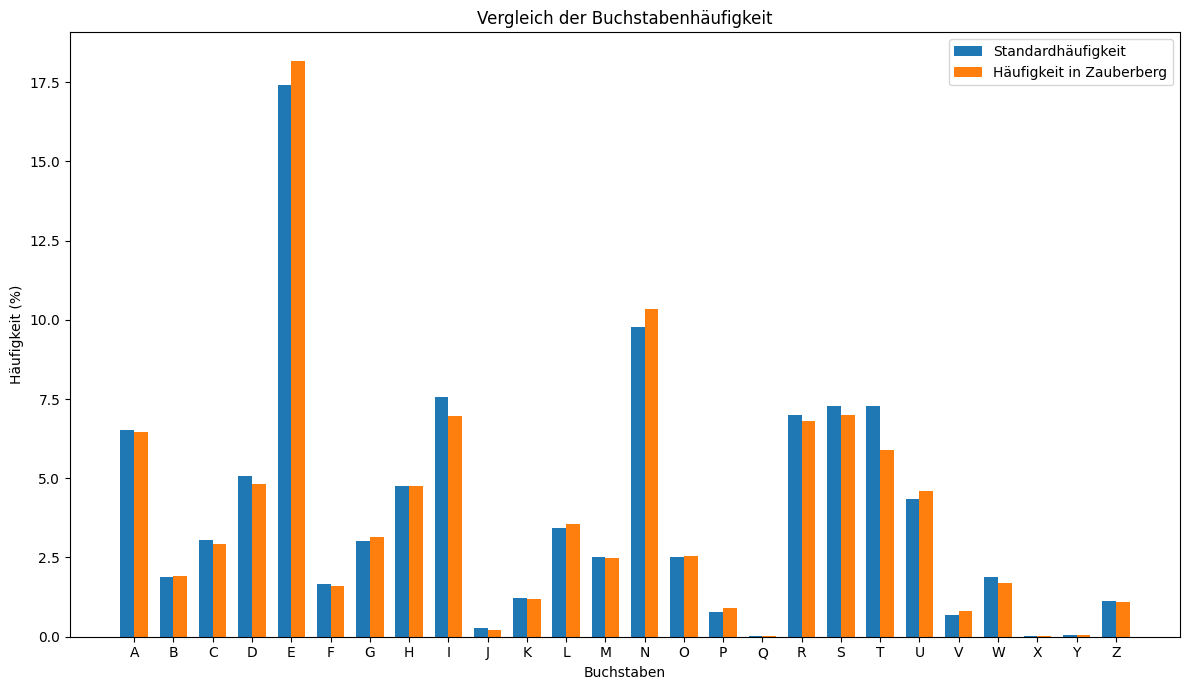
\includegraphics[keepaspectratio]{files/250919_vigenere/vigenere_files/figure-pdf/cell-2-output-1.png}}

Die Grafik zeigt, dass bei einer Textlänge von 51'396 Buchstaben die
Verteilung in einem literarischen Text nahezu identisch ist mit der
allgemeinen Häufigkeitsverteilung in der deutschen Sprache.

Die nächste Grafik zeigt, was mit der Verteilung der Buchstaben
geschieht, wenn der gleiche Text mit einer Caesar-Chiffre verschlüsselt
worden ist.

\begin{Shaded}
\begin{Highlighting}[numbers=left,,]
\KeywordTok{def}\NormalTok{ caesar(text : }\BuiltInTok{str}\NormalTok{, shift : }\BuiltInTok{int}\NormalTok{, encrypt}\OperatorTok{=}\VariableTok{True}\NormalTok{) }\OperatorTok{{-}\textgreater{}} \BuiltInTok{str}\NormalTok{:}
\NormalTok{    text }\OperatorTok{=}\NormalTok{ text.upper()}
\NormalTok{    result }\OperatorTok{=} \StringTok{""}
    
    \ControlFlowTok{if}\NormalTok{ encrypt:}
        \ControlFlowTok{for}\NormalTok{ char }\KeywordTok{in}\NormalTok{ text:}
\NormalTok{            shifted }\OperatorTok{=}\NormalTok{ (}\BuiltInTok{ord}\NormalTok{(char) }\OperatorTok{{-}} \BuiltInTok{ord}\NormalTok{(}\StringTok{\textquotesingle{}A\textquotesingle{}}\NormalTok{) }\OperatorTok{+}\NormalTok{ shift) }\OperatorTok{\%} \DecValTok{26} \OperatorTok{+} \BuiltInTok{ord}\NormalTok{(}\StringTok{\textquotesingle{}A\textquotesingle{}}\NormalTok{)}
\NormalTok{            result }\OperatorTok{+=} \BuiltInTok{chr}\NormalTok{(shifted)}
    \ControlFlowTok{else}\NormalTok{:}
        \ControlFlowTok{for}\NormalTok{ char }\KeywordTok{in}\NormalTok{ text:}
\NormalTok{            shifted }\OperatorTok{=}\NormalTok{ (}\BuiltInTok{ord}\NormalTok{(char) }\OperatorTok{{-}} \BuiltInTok{ord}\NormalTok{(}\StringTok{\textquotesingle{}A\textquotesingle{}}\NormalTok{) }\OperatorTok{{-}}\NormalTok{ shift) }\OperatorTok{\%} \DecValTok{26} \OperatorTok{+} \BuiltInTok{ord}\NormalTok{(}\StringTok{\textquotesingle{}A\textquotesingle{}}\NormalTok{)}
\NormalTok{            result }\OperatorTok{+=} \BuiltInTok{chr}\NormalTok{(shifted)}
            
    \ControlFlowTok{return}\NormalTok{ result}


\NormalTok{zauberberg\_verschluesselt }\OperatorTok{=}\NormalTok{ caesar(zauberberg, }\DecValTok{11}\NormalTok{, encrypt}\OperatorTok{=}\VariableTok{True}\NormalTok{)}
\NormalTok{frequency\_zauberberg\_verschluesselt }\OperatorTok{=}\NormalTok{ letter\_frequency(zauberberg\_verschluesselt)}
\NormalTok{dft[}\StringTok{\textquotesingle{}Zauberberg Frequency Encrypted\textquotesingle{}}\NormalTok{] }\OperatorTok{=}\NormalTok{ pd.Series(frequency\_zauberberg\_verschluesselt)}

\CommentTok{\# {-}{-}{-} Erstellen Sie das Side{-}by{-}Side{-}Balkendiagramm {-}{-}{-}}
\CommentTok{\# Legen Sie die Breite der Balken fest}
\NormalTok{bar\_width }\OperatorTok{=} \FloatTok{0.35}

\CommentTok{\# Verwenden Sie den Index des transponierten DataFrames (dft)}
\NormalTok{x }\OperatorTok{=}\NormalTok{ np.arange(}\BuiltInTok{len}\NormalTok{(dft.index))}

\NormalTok{fig, ax }\OperatorTok{=}\NormalTok{ plt.subplots(figsize}\OperatorTok{=}\NormalTok{(}\DecValTok{12}\NormalTok{, }\DecValTok{7}\NormalTok{))}

\CommentTok{\# Zeichnen Sie die Balken für die beiden Spalten aus dft}
\NormalTok{ax.bar(x }\OperatorTok{{-}}\NormalTok{ bar\_width}\OperatorTok{/}\DecValTok{2}\NormalTok{, dft[}\StringTok{\textquotesingle{}Standard Frequency\textquotesingle{}}\NormalTok{], bar\_width, label}\OperatorTok{=}\StringTok{\textquotesingle{}Standardhäufigkeit\textquotesingle{}}\NormalTok{)}
\NormalTok{ax.bar(x }\OperatorTok{+}\NormalTok{ bar\_width}\OperatorTok{/}\DecValTok{2}\NormalTok{, dft[}\StringTok{\textquotesingle{}Zauberberg Frequency Encrypted\textquotesingle{}}\NormalTok{], bar\_width, label}\OperatorTok{=}\StringTok{\textquotesingle{}Häufigkeit Zauberberg veschlüsselt\textquotesingle{}}\NormalTok{)}

\NormalTok{ax.set\_xticks(x)}
\NormalTok{ax.set\_xticklabels(dft.index)}

\NormalTok{ax.set\_xlabel(}\StringTok{\textquotesingle{}Buchstaben\textquotesingle{}}\NormalTok{)}
\NormalTok{ax.set\_ylabel(}\StringTok{\textquotesingle{}Häufigkeit (\%)\textquotesingle{}}\NormalTok{)}
\NormalTok{ax.set\_title(}\StringTok{\textquotesingle{}Vergleich der Buchstabenhäufigkeit im verschlüsselten Text\textquotesingle{}}\NormalTok{)}
\NormalTok{ax.legend()}
\NormalTok{plt.tight\_layout()}

\NormalTok{plt.show()}
\end{Highlighting}
\end{Shaded}

\pandocbounded{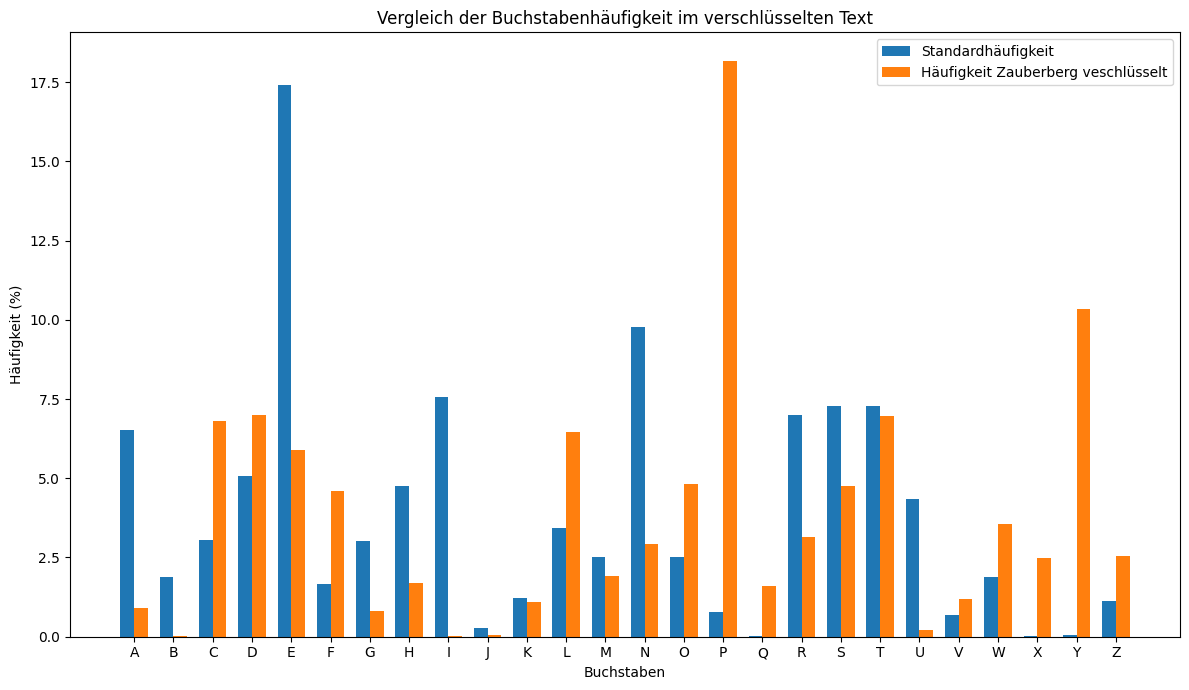
\includegraphics[keepaspectratio]{files/250919_vigenere/vigenere_files/figure-pdf/cell-3-output-1.png}}

Es ist deutlich zu erkennen, dass die Verteilung dem gleichen Muster
folgt - verschoben um elf Positionen. Diese Auswertung ermöglicht die
Entschlüsselung des Textes, ohne alle möglichen Schlüsselalphabete
durchzuprobieren.

\section{Vigenère Chiffre}\label{vigenuxe8re-chiffre-1}

Bei der Vigenère Chiffre handelt es sich um eine polyalphabetische
Chiffre. Das Verfahren ist nach Blaise de Vigenère (1523 - 1596)
benannt. Polyalphabetisch heisst, dass zur Verschlüsselung nicht eine
Verschiebung vorgenommen wird, sondern - nach jedem Buchstaben wechselnd
- mehrere Verschiebungen vorgenommen werden.

Um das zu erreichen, verwendet man ein sogenanntes Vigenère-Quadrat wie
unten abgebildet.

\pandocbounded{
\includegraphics[keepaspectratio]{index_files/mediabag/files/250919_vigenere/vigenere_square_shading.pdf}}

Für die Verschlüsselung eines Klartextes braucht das Vigenère Verfahren
ein Schlüsselwort. Das Schlüsselwort sollte möglichst lang sein. Das
folgende Beispiel soll zeigen, wie das Vigenère Verfahren funktioniert.
Der zu verschlüsselnde Klartext lautet `Kryptologie ist spannend' und
der Schlüssel `Buelrain'. Als Hilfestellung werden Text und Schlüssel in
einer Tabelle dargestellt.

\begin{verbatim}
kryptologieistspannend
buelrainbuelrainbuelra
\end{verbatim}

Der Schlüssel wird dabei ohne Wortabstand so oft wiederholt, bis die
Buchstabenfolge des Schlüssels gleich lang ist, wie die Buchstabenfolge,
welche zu verschlüsseln ist.\\
Als nächstes wird der zu verschlüsselnde Buchstabe in der Kopfzeile des
Vigenère Quadrates gesucht. Damit wird die Spalte mit dem verschobenen
Alphabet identifiziert. Der chiffrierte Buchstabe ergibt sich, indem in
der Spalte mit den Zeilenköpfen der unter dem zu chiffrierenden
Buchstaben befindliche Buchstabe des Schlüssels gesucht wird. Der
Schnittpunkt der Zeile mit der vorher gefundenen Spalte entspricht dem
chiffrierten Buchstaben.

\begin{verbatim}
kryptologieistspannend
buelrainbuelrainbuelra

LLCAKOTBHCITJTACBHRPED
\end{verbatim}

Alternativ kann eine Verschlüsselung mit der Vigenère Chiffre auch mit
modularer Arithmetik umgesetzt werden. Dazu wird jedem Buchstaben ein
Zahlenwert nach dem Muster \(a = 0, b = 1, ... , z = 25\) zugewiesen.
Die Verschlüsselung erfolgt anschliessend nach der `Formel'
\(C_i = (P_i + K_i)\ mod\ 26\) Wobei die Buchstaben \(C\) für den
chiffrierten Text, \(P\) für den Klartext (Englisch \emph{plain text})
und \(K\) für den Schlüssel (Englisch \emph{key}) stehen. Der Index
\(_i\) steht für den \(i\)-ten Buchstaben in der Textfolge.

Das obige Beispiel stellt sich dann folgendermassen dar:

\begin{verbatim}
 k  r  y  p  t  o  l  o  g  i  e  i  s  t  s  p  a  n  n  e  n  d
10 17 24 15 19 14 11 14 06 08 04 08 18 19 18 15 00 13 13 04 13 03
 b  u  e  l  r  a  i  n  b  u  e  l  r  a  i  n  b  u  e  l  r  a
01 20 04 11 17 00 08 13 01 20 04 11 17 00 08 13 01 20 04 11 17 00

11 37 28 26 36 14 19 27 07 28 08 19 35 19 26 28 01 33 17 15 30 03

11 11 02 00 10 14 19 01 07 02 08 19 09 19 00 02 01 07 17 15 04 03
 L  L  C  A  K  O  T  B  H  C  I  T  J  T  A  C  B  H  R  P  E  D
\end{verbatim}

Für die Entschlüsselung wird die `Formel' folgendermassen umgekehrt:
\(P_i = (C_i - K_i + 26)\ mod\ 26\). Die Addition von 26 in der Klammer
erfolgt, um negative Zahlen zu vermeiden.

Wie sich die Vigenère Verschlüsselung auf die Verteilung der Buchstaben
auswirkt, kann untenstehender Grafik entnommen werden.

\begin{Shaded}
\begin{Highlighting}[numbers=left,,]
\KeywordTok{def}\NormalTok{ vigenere\_chiffre(text: }\BuiltInTok{str}\NormalTok{, key: }\BuiltInTok{str}\NormalTok{, encrypt}\OperatorTok{=}\VariableTok{True}\NormalTok{) }\OperatorTok{{-}\textgreater{}} \BuiltInTok{str}\NormalTok{:}
    \CommentTok{"""}
\CommentTok{    Implementiert die Vigenère{-}Verschlüsselung für einen gegebenen Klartext und}
\CommentTok{    Schlüssel.}
\CommentTok{    }
\CommentTok{    Args:}
\CommentTok{        klartext (str): Der zu verschlüsselnde Text schluessel (str): Das}
\CommentTok{        Schlüsselwort für die Verschlüsselung}
\CommentTok{    }
\CommentTok{    Returns:}
\CommentTok{        str: Der verschlüsselte Text}
\CommentTok{    """}
    
    \CommentTok{\# initialisiere den resultierenden Text}
\NormalTok{    resulting\_text }\OperatorTok{=} \StringTok{\textquotesingle{}\textquotesingle{}}
    
    \CommentTok{\# bestimme die Schlüssellänge für die anschliessende Modulo{-}Operation}
\NormalTok{    key\_length }\OperatorTok{=} \BuiltInTok{len}\NormalTok{(key)}
    
    \CommentTok{\# itererie über den Eingabetext unter gleichzeitiger Erfassung des Index}
    \ControlFlowTok{for}\NormalTok{ i, char }\KeywordTok{in} \BuiltInTok{enumerate}\NormalTok{(text):}
        \CommentTok{\# berechne den Zahlwert des Buchstabens aus der ascii Tabelle}
\NormalTok{        char\_no }\OperatorTok{=} \BuiltInTok{ord}\NormalTok{(char) }\OperatorTok{{-}} \DecValTok{97}
\NormalTok{        key\_no }\OperatorTok{=} \BuiltInTok{ord}\NormalTok{(key[i }\OperatorTok{\%}\NormalTok{ key\_length]) }\OperatorTok{{-}} \DecValTok{97}
        
        \ControlFlowTok{if}\NormalTok{ encrypt }\OperatorTok{==} \VariableTok{True}\NormalTok{:}
            \CommentTok{\# berechne den Zahlwert des verschlüsselten Buchstabens}
\NormalTok{            ciph\_no }\OperatorTok{=}\NormalTok{ (char\_no }\OperatorTok{+}\NormalTok{ key\_no) }\OperatorTok{\%} \DecValTok{26}
        \ControlFlowTok{else}\NormalTok{:}
            \CommentTok{\# berechne den Zahlwert des entschlüsselten Buchstabens}
\NormalTok{            ciph\_no }\OperatorTok{=}\NormalTok{ (char\_no }\OperatorTok{+}\NormalTok{ (}\DecValTok{26} \OperatorTok{{-}}\NormalTok{ key\_no)) }\OperatorTok{\%} \DecValTok{26}
            
         \CommentTok{\# übernehme das Zeichen aufgrund seines Zahlwertes aus der ascii Tabelle  }
\NormalTok{        ciph }\OperatorTok{=} \BuiltInTok{chr}\NormalTok{(ciph\_no }\OperatorTok{+} \DecValTok{97}\NormalTok{)}
        
        \CommentTok{\# füge den Buchstaben am resultierenden Text an}
\NormalTok{        resulting\_text }\OperatorTok{+=}\NormalTok{ ciph}
    \ControlFlowTok{return}\NormalTok{ resulting\_text}

\NormalTok{zauberberg\_vigenere }\OperatorTok{=}\NormalTok{ vigenere\_chiffre(zauberberg.lower(), }\StringTok{\textquotesingle{}buelrain\textquotesingle{}}\NormalTok{, encrypt}\OperatorTok{=}\VariableTok{True}\NormalTok{)}

\NormalTok{zauberberg\_vigenere\_frequency }\OperatorTok{=}\NormalTok{ letter\_frequency(zauberberg\_vigenere.upper())}
\NormalTok{dft[}\StringTok{\textquotesingle{}Zauberberg Frequency Vigenere\textquotesingle{}}\NormalTok{] }\OperatorTok{=}\NormalTok{ pd.Series(zauberberg\_vigenere\_frequency)}

\CommentTok{\# {-}{-}{-} Erstellen Sie das Side{-}by{-}Side{-}Balkendiagramm {-}{-}{-}}
\CommentTok{\# Legen Sie die Breite der Balken fest}
\NormalTok{bar\_width }\OperatorTok{=} \FloatTok{0.35}

\CommentTok{\# Verwenden Sie den Index des transponierten DataFrames (dft)}
\NormalTok{x }\OperatorTok{=}\NormalTok{ np.arange(}\BuiltInTok{len}\NormalTok{(dft.index))}

\NormalTok{fig, ax }\OperatorTok{=}\NormalTok{ plt.subplots(figsize}\OperatorTok{=}\NormalTok{(}\DecValTok{12}\NormalTok{, }\DecValTok{7}\NormalTok{))}

\CommentTok{\# Zeichnen Sie die Balken für die beiden Spalten aus dft}
\NormalTok{ax.bar(x }\OperatorTok{{-}}\NormalTok{ bar\_width}\OperatorTok{/}\DecValTok{2}\NormalTok{, dft[}\StringTok{\textquotesingle{}Standard Frequency\textquotesingle{}}\NormalTok{], bar\_width, label}\OperatorTok{=}\StringTok{\textquotesingle{}Standardhäufigkeit\textquotesingle{}}\NormalTok{)}
\NormalTok{ax.bar(x }\OperatorTok{+}\NormalTok{ bar\_width}\OperatorTok{/}\DecValTok{2}\NormalTok{, dft[}\StringTok{\textquotesingle{}Zauberberg Frequency Vigenere\textquotesingle{}}\NormalTok{], bar\_width, label}\OperatorTok{=}\StringTok{\textquotesingle{}Häufigkeit Zauberberg Vigenère\textquotesingle{}}\NormalTok{)}

\NormalTok{ax.set\_xticks(x)}
\NormalTok{ax.set\_xticklabels(dft.index)}

\NormalTok{ax.set\_xlabel(}\StringTok{\textquotesingle{}Buchstaben\textquotesingle{}}\NormalTok{)}
\NormalTok{ax.set\_ylabel(}\StringTok{\textquotesingle{}Häufigkeit (\%)\textquotesingle{}}\NormalTok{)}
\NormalTok{ax.set\_title(}\StringTok{\textquotesingle{}Vergleich der Buchstabenhäufigkeit im Vigenère verschlüsselten Text\textquotesingle{}}\NormalTok{)}
\NormalTok{ax.legend()}
\NormalTok{plt.tight\_layout()}

\NormalTok{plt.show()}
\end{Highlighting}
\end{Shaded}

\pandocbounded{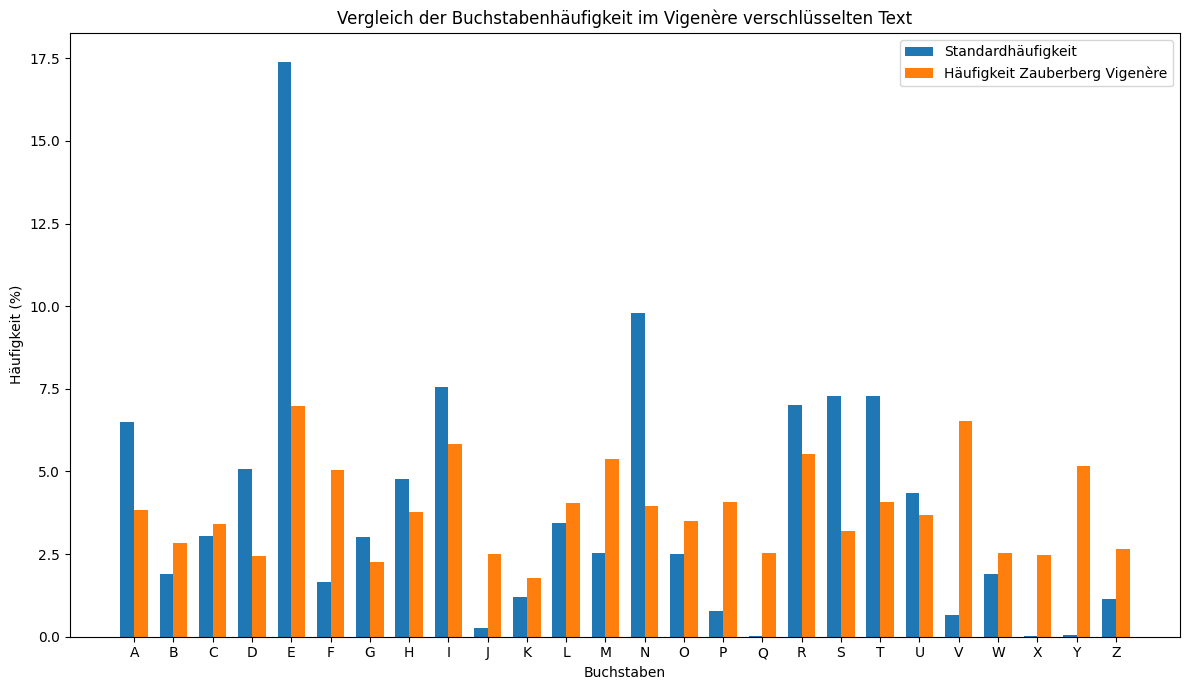
\includegraphics[keepaspectratio]{files/250919_vigenere/vigenere_files/figure-pdf/cell-4-output-1.png}}

Wie unschwer zu erkennen ist, stellt sich die Verteilung der Buchstaben
in einem polyalphabetisch verschlüsselten Text deutlich anders dar, als
dies in normalen Text der Fall ist. Die Vigenère Chiffre galt daher
während ungefähr 300 Jahren als `la chiffre indéchiffrable'.

Ein Spezialfall der Vigenère-Chiffre lässt sich tatsächlich nicht
entschlüsseln. Das ist dann der Fall, wenn der Schlüssel länger ist als
der Klartext. Man spricht in diesem Fall vom One-Time Pad.

\chapter{Vigenère Chiffre Implementierung in
Python}\label{vigenuxe8re-chiffre-implementierung-in-python}

In diesem Notebook wird eine mögliche Implementierung der Vigenère
Chiffre in Python vorgestellt.

\begin{Shaded}
\begin{Highlighting}[numbers=left,,]
\KeywordTok{def}\NormalTok{ vigenere(text: }\BuiltInTok{str}\NormalTok{, key: }\BuiltInTok{str}\NormalTok{, mode: }\BuiltInTok{str}\NormalTok{) }\OperatorTok{{-}\textgreater{}} \BuiltInTok{str}\NormalTok{:}
    \CommentTok{"""Encrypts or decrypts a given text using the Vigenère cipher.}

\CommentTok{    The function processes a string of uppercase alphabetic characters}
\CommentTok{    using a provided key for encryption or decryption.}

\CommentTok{    Args:}
\CommentTok{        text: The string to be encrypted or decrypted. It should only contain}
\CommentTok{              uppercase alphabetic characters (A{-}Z).}
\CommentTok{        key: The key for the cipher. It should also only contain}
\CommentTok{             uppercase alphabetic characters (A{-}Z).}
\CommentTok{        mode: The operation to perform, must be \textquotesingle{}encrypt\textquotesingle{} or \textquotesingle{}decrypt\textquotesingle{}.}

\CommentTok{    Returns:}
\CommentTok{        The resulting ciphertext or plaintext.}

\CommentTok{    Raises:}
\CommentTok{        ValueError: If the mode is not \textquotesingle{}encrypt\textquotesingle{} or \textquotesingle{}decrypt\textquotesingle{}.}
\CommentTok{    """}

    \CommentTok{\# Ensure the mode is valid before proceeding.}
    \ControlFlowTok{if}\NormalTok{ mode }\KeywordTok{not} \KeywordTok{in}\NormalTok{ [}\StringTok{\textquotesingle{}encrypt\textquotesingle{}}\NormalTok{, }\StringTok{\textquotesingle{}decrypt\textquotesingle{}}\NormalTok{]:}
        \ControlFlowTok{raise} \PreprocessorTok{ValueError}\NormalTok{(}\StringTok{"Mode must be \textquotesingle{}encrypt\textquotesingle{} or \textquotesingle{}decrypt\textquotesingle{}"}\NormalTok{)}
    
\NormalTok{    key\_length }\OperatorTok{=} \BuiltInTok{len}\NormalTok{(key)}
    
    \ControlFlowTok{if}\NormalTok{ mode }\OperatorTok{==} \StringTok{\textquotesingle{}encrypt\textquotesingle{}}\NormalTok{:}
\NormalTok{       cipher }\OperatorTok{=} \StringTok{\textquotesingle{}\textquotesingle{}}
       \CommentTok{\# Iterate through each character of the input text.}
       \ControlFlowTok{for}\NormalTok{ i, char }\KeywordTok{in} \BuiltInTok{enumerate}\NormalTok{(text):}
           \CommentTok{\# Convert the current text character and the corresponding key }
           \CommentTok{\# character to a number (0{-}25).}
           \CommentTok{\# The key character is determined using modulo to cycle through }
           \CommentTok{\# the key.}
\NormalTok{           char\_num }\OperatorTok{=} \BuiltInTok{ord}\NormalTok{(char) }\OperatorTok{{-}} \BuiltInTok{ord}\NormalTok{(}\StringTok{\textquotesingle{}A\textquotesingle{}}\NormalTok{)}
\NormalTok{           key\_num }\OperatorTok{=} \BuiltInTok{ord}\NormalTok{(key[i }\OperatorTok{\%}\NormalTok{ key\_length]) }\OperatorTok{{-}} \BuiltInTok{ord}\NormalTok{(}\StringTok{\textquotesingle{}A\textquotesingle{}}\NormalTok{)}
           
           \CommentTok{\# Calculate the new character\textquotesingle{}s number using the Vigenère encryption formula.}
           \CommentTok{\# The modulo operator ensures the result stays within the range 0{-}25.}
\NormalTok{           cipher\_num }\OperatorTok{=}\NormalTok{ (char\_num }\OperatorTok{+}\NormalTok{ key\_num) }\OperatorTok{\%} \DecValTok{26}
           
           \CommentTok{\# Convert the resulting number back to an uppercase character and append it.}
\NormalTok{           cipher }\OperatorTok{+=} \BuiltInTok{chr}\NormalTok{(cipher\_num }\OperatorTok{+} \BuiltInTok{ord}\NormalTok{(}\StringTok{\textquotesingle{}A\textquotesingle{}}\NormalTok{))}
       \ControlFlowTok{return}\NormalTok{ cipher  }
    \ControlFlowTok{else}\NormalTok{:  }\CommentTok{\# mode == \textquotesingle{}decrypt\textquotesingle{}}
\NormalTok{        plain }\OperatorTok{=} \StringTok{\textquotesingle{}\textquotesingle{}}
        \CommentTok{\# Iterate through each character of the input text.}
        \ControlFlowTok{for}\NormalTok{ i, char }\KeywordTok{in} \BuiltInTok{enumerate}\NormalTok{(text):}
            \CommentTok{\# Convert the current text character and the corresponding key }
            \CommentTok{\# character to a number (0{-}25).}
\NormalTok{            char\_num }\OperatorTok{=} \BuiltInTok{ord}\NormalTok{(char) }\OperatorTok{{-}} \BuiltInTok{ord}\NormalTok{(}\StringTok{\textquotesingle{}A\textquotesingle{}}\NormalTok{)}
\NormalTok{            key\_num }\OperatorTok{=} \BuiltInTok{ord}\NormalTok{(key[i }\OperatorTok{\%}\NormalTok{ key\_length]) }\OperatorTok{{-}} \BuiltInTok{ord}\NormalTok{(}\StringTok{\textquotesingle{}A\textquotesingle{}}\NormalTok{)}
            
            \CommentTok{\# Calculate the new character\textquotesingle{}s number using the Vigenère }
            \CommentTok{\# decryption formula.}
            \CommentTok{\# The modulo operator handles negative results, ensuring the }
            \CommentTok{\# result is correct.}
\NormalTok{            plain\_num }\OperatorTok{=}\NormalTok{ (char\_num }\OperatorTok{{-}}\NormalTok{ key\_num) }\OperatorTok{\%} \DecValTok{26}
            
            \CommentTok{\# Convert the resulting number back to an uppercase }
            \CommentTok{\# character and append it.}
\NormalTok{            plain }\OperatorTok{+=} \BuiltInTok{chr}\NormalTok{(plain\_num }\OperatorTok{+} \BuiltInTok{ord}\NormalTok{(}\StringTok{\textquotesingle{}A\textquotesingle{}}\NormalTok{))}
        \ControlFlowTok{return}\NormalTok{ plain}
\end{Highlighting}
\end{Shaded}

Die Funktion \texttt{vigenere()} wird im Folgenden detailliert erklärt.

Die Signatur der Funktion

\begin{Shaded}
\begin{Highlighting}[numbers=left,,]
\KeywordTok{def}\NormalTok{ vigenere(text: }\BuiltInTok{str}\NormalTok{, key: }\BuiltInTok{str}\NormalTok{, mode: }\BuiltInTok{str}\NormalTok{) }\OperatorTok{{-}\textgreater{}} \BuiltInTok{str}\NormalTok{:}
\end{Highlighting}
\end{Shaded}

zeigt, dass die Funktion drei Parameter erwartet: * \texttt{text}: Der
zu verschlüsselnde oder zu entschlüsselnde Text als String. *
\texttt{key}: Der Schlüssel zur Verschlüsselung oder Entschlüsselung als
String. * \texttt{mode}: Der Modus, der angibt, ob der Text
verschlüsselt oder entschlüsselt werden soll. Mögliche Werte sind
\texttt{\textquotesingle{}encrypt\textquotesingle{}} für Verschlüsselung
und \texttt{\textquotesingle{}decrypt\textquotesingle{}} für
Entschlüsselung (dies ist allerdings nicht direkt aus der Signatur
ersichtlich).

Anschliessend an die Signatur folgt ein ausführlicher Docstring, der die
Funktion und ihre Parameter beschreibt. Dieser ist - obwohl in Englisch
abgefasst - aus sich selber heraus verständlich.

Der Docstring wird gefolgt durch die Prüfung, ob zulässige Werte für den
\texttt{mode}-Parameter übergeben wurden. Ist dies nicht der Fall, wird
eine \texttt{ValueError}-Exception ausgelöst.

\begin{Shaded}
\begin{Highlighting}[numbers=left,,]
\ControlFlowTok{if}\NormalTok{ mode }\KeywordTok{not} \KeywordTok{in}\NormalTok{ [}\StringTok{\textquotesingle{}encrypt\textquotesingle{}}\NormalTok{, }\StringTok{\textquotesingle{}decrypt\textquotesingle{}}\NormalTok{]:}
    \ControlFlowTok{raise} \PreprocessorTok{ValueError}\NormalTok{(}\StringTok{"Mode must be \textquotesingle{}encrypt\textquotesingle{} or \textquotesingle{}decrypt\textquotesingle{}"}\NormalTok{)}
\end{Highlighting}
\end{Shaded}

Um diese Prüfung durchzuführen, werden die zulässigen Werte in einer
Liste zur Verfügung gestellt. Geprüft wird dann, ob der \texttt{mode}
zugewiesene Wert in der Liste enthalten ist. Falls dies nicht der Fall
ist, wird eine Fehlermeldung ausgegeben und die Ausführung der Funktion
abgebrochen.

Sofern der \texttt{mode}-Parameter einen zulässigen Wert enthält,
beginnt die eigentliche Funktionslogik zu spielen.

Als erstes wird die Länge des Schlüssels in

\begin{Shaded}
\begin{Highlighting}[numbers=left,,]
\NormalTok{key\_length }\OperatorTok{=} \BuiltInTok{len}\NormalTok{(key)}
\end{Highlighting}
\end{Shaded}

der Variablen \texttt{key\_length} zugewiesen. Diese Information wird
weiter unten benötigt, um in einer besonderen Art von Schlaufe über den
Text des Schlüssels zu iterieren.

Nach dieser Zuweisung teilt sich die Funktion in die Zweige Ver- bzw.
Entschlüsselung.

Zuerst wird die Verschlüsselung - eingeleitet mit
\texttt{if\ mode\ ==\ \textquotesingle{}encrypt\textquotesingle{}:} -
betrachtet.

Innerhalb dieses Blocks wird als erstes ein leerer String
\texttt{cipher} initialisiert, der später die verschlüsselten Zeichen
aufnehmen wird.

Anschliessend wird mit einer \texttt{for}-Schlaufe über den zu
verschlüsselnden Text iteriert.

\begin{Shaded}
\begin{Highlighting}[numbers=left,,]
\ControlFlowTok{for}\NormalTok{ i, char }\KeywordTok{in} \BuiltInTok{enumerate}\NormalTok{(text):}
\end{Highlighting}
\end{Shaded}

In dieser Schlaufe wird die Funktion \texttt{enumerate()} verwendet.
Diese Funktion liefert ein Tupel aus Index und dem jeweiligen Element
der Struktur, über die iteriert wird. Die Werte des Tupels werden den
Variablen \texttt{i} und \texttt{char} zugewiesen.

Die Variabeln \texttt{i} und \texttt{char} werden innerhalb der Schlaufe
verwendet, um die einzelnen Zeichen des Textes in eine Zahl umzuwandeln.

\begin{Shaded}
\begin{Highlighting}[numbers=left,,]
\NormalTok{    char\_num }\OperatorTok{=} \BuiltInTok{ord}\NormalTok{(char) }\OperatorTok{{-}} \BuiltInTok{ord}\NormalTok{(}\StringTok{\textquotesingle{}A\textquotesingle{}}\NormalTok{)}
\NormalTok{    key\_num }\OperatorTok{=} \BuiltInTok{ord}\NormalTok{(key[i }\OperatorTok{\%}\NormalTok{ key\_length]) }\OperatorTok{{-}} \BuiltInTok{ord}\NormalTok{(}\StringTok{\textquotesingle{}A\textquotesingle{}}\NormalTok{)}
\end{Highlighting}
\end{Shaded}

Die Funktion \texttt{ord()} wandelt einen Buchstaben in die
entsprechende Zahl aus der ASCII-Tabelle um. Damit die Zahlen im Bereich
von 0 bis 25 liegen, wird der ASCII-Wert des Buchstabens `A' abgezogen.
Der Buchstabe `A' wird verwendet, da die zu verschlüsselnden Zeichen in
Grossbuchstaben vorgegeben sind.\\
Da der Schlüssel kürzer als der zu verschlüsselnde Text sein kann, wird
mit \texttt{i\ \%\ key\_length} über den Schlüssel iteriert. Der
Modulo-Operator \texttt{\%} sorgt dafür, dass der Index Wert des
verwendeten Index immer zwischen 0 und der Länge des Schlüssels
\texttt{key\_length} bleibt. Dadurch wird sichergestellt, dass der
Schlüssel wieder von vorne begonnen wird, sobald das Ende des Schlüssels
erreicht ist. Anschliessend wird mit den einzelnen Buchstaben des
Schlüssels genauso verfahren wie mit den Buchstaben des Textes.

Nachdem die Buchstaben des Textes sowie des Schlüssels in Zahlen
umgewandelt wurden, wird die eigentliche Verschlüsselung gemäss der
Formel \(C_i = (P_i + K_i)\ mod\ 26\) durchgeführt.

\begin{Shaded}
\begin{Highlighting}[numbers=left,,]
\NormalTok{    cipher\_num }\OperatorTok{=}\NormalTok{ (char\_num }\OperatorTok{+}\NormalTok{ key\_num) }\OperatorTok{\%} \DecValTok{26}
\end{Highlighting}
\end{Shaded}

Die Zahlenwerte des verschlüsselten Textes werden anschliessend wieder
in Buchstaben umgewandelt und an den String \texttt{cipher} angehängt.
Dazu wird die Funktion \texttt{chr()} verwendet, die eine Zahl in den
entsprechenden Buchstaben der ASCII-Tabelle umwandelt. Da die
Zahlenwerte im Bereich von 0 bis 25 liegen, wird der ASCII-Wert des
Buchstabens `A' addiert.

\begin{Shaded}
\begin{Highlighting}[numbers=left,,]
\NormalTok{    cipher }\OperatorTok{+=} \BuiltInTok{chr}\NormalTok{(cipher\_num }\OperatorTok{+} \BuiltInTok{ord}\NormalTok{(}\StringTok{\textquotesingle{}A\textquotesingle{}}\NormalTok{))}
\end{Highlighting}
\end{Shaded}

Der unter \texttt{cipher} abgelegte String wird am Ende des Blocks
zurückgegeben.

Im zweiten Block wird die Entschlüsselung - eingeleitet mit
\texttt{else:} - durchgeführt. Der Prozess ist dem der Verschlüsselung
sehr ähnlich, jedoch wird hier die umgekehrte Formel
(\(P_i = (C_i - K_i + 26)\ mod\
26\)) verwendet.

\begin{Shaded}
\begin{Highlighting}[numbers=left,,]
\NormalTok{    plain\_num }\OperatorTok{=}\NormalTok{ (char\_num }\OperatorTok{{-}}\NormalTok{ key\_num }\OperatorTok{+} \DecValTok{26}\NormalTok{) }\OperatorTok{\%} \DecValTok{26}
\NormalTok{    plain }\OperatorTok{+=} \BuiltInTok{chr}\NormalTok{(plain\_num }\OperatorTok{+} \BuiltInTok{ord}\NormalTok{(}\StringTok{\textquotesingle{}A\textquotesingle{}}\NormalTok{))}
\end{Highlighting}
\end{Shaded}

Alles andere entspricht dem Vorgehen bei der Verschlüsselung.

\chapter{Die Vigenère-Verschlüsselung
brechen}\label{die-vigenuxe8re-verschluxfcsselung-brechen}

Die entscheidende Schwäche der Vigenère-Verschlüsselung wurde Mitte des
19. Jahrhunderts von zwei Männern unabhängig voneinander entdeckt. Einer
von ihnen war Charles Babbage, ein britischer Universalgelehrter. Er
entdeckte die Schwachstelle, um eine Wette zu gewinnen. Der andere war
Friedrich Wilhelm Kasiski, ein pensionierter Major der preußischen
Armee, der nach seiner Pensionierung seine Zeit mit Schreiben
verbrachte. Die Methode zum Brechen der Vigenère-Verschlüsselung ist
nach dem preußischen Major Kasiski benannt.

\section{Die Kasiski-Methode --
Zusammenfassung}\label{die-kasiski-methode-zusammenfassung}

Die \textbf{Kasiski-Methode} ist eine Technik zum Brechen der
Vigenère-Verschlüsselung, bei der wiederholte Muster im Geheimtext
ausgenutzt werden. So funktioniert sie:

\subsection{Grundprinzip}\label{grundprinzip}

Wenn dieselbe Klartextsequenz mit demselben Teil des Schlüssels
verschlüsselt wird, entstehen identische Geheimtextsequenzen. Indem wir
diese Wiederholungen finden, können wir die Schlüssellänge bestimmen.

\subsection{Schritt-für-Schritt-Anleitung}\label{schritt-fuxfcr-schritt-anleitung}

\begin{enumerate}
\def\labelenumi{\arabic{enumi}.}
\tightlist
\item
  \textbf{Wiederholte Sequenzen finden}

  \begin{itemize}
  \tightlist
  \item
    Den Geheimtext nach identischen Sequenzen von 3+ Zeichen
    durchsuchen.
  \item
    Die Positionen aufzeichnen, an denen diese Sequenzen auftreten.
  \end{itemize}
\item
  \textbf{Abstände berechnen}

  \begin{itemize}
  \tightlist
  \item
    Den Abstand zwischen wiederholten Sequenzen messen.
  \item
    Die Schlüssellänge muss ein Teiler dieser Abstände sein.
  \end{itemize}
\item
  \textbf{Schlüssellänge bestimmen}

  \begin{itemize}
  \tightlist
  \item
    Den größten gemeinsamen Teiler (ggT) aller Abstände finden.
  \item
    Oder nach dem häufigsten gemeinsamen Teiler suchen.
  \item
    Dies ergibt die wahrscheinliche Schlüssellänge.
  \end{itemize}
\item
  \textbf{Häufigkeitsanalyse}

  \begin{itemize}
  \tightlist
  \item
    Den Geheimtext basierend auf der Schlüssellänge in Gruppen
    aufteilen.
  \item
    Jede Gruppe wurde mit demselben Schlüsselzeichen verschlüsselt.
  \item
    Eine Häufigkeitsanalyse auf jede Gruppe separat anwenden.
  \item
    Die Buchstabenhäufigkeiten mit den erwarteten Mustern der Sprache
    abgleichen.
  \end{itemize}
\end{enumerate}

\subsection{Beispiel}\label{beispiel}

Wenn „THE`` mehrmals im Klartext an Positionen erscheint, an denen sich
der Schlüssel wiederholt, sind die entsprechenden Geheimtextsequenzen
identisch. Wenn diese Sequenzen 10 Positionen voneinander entfernt sind,
ist die Schlüssellänge wahrscheinlich ein Teiler von 10 (1, 2, 5 oder
10).

Für ein konstruiertes Beispiel, wenn der Klartext „the codes in the word
and the message`` lautet und der Schlüssel „crypt`` ist, erhalten wir
den folgenden Geheimtext.

\begin{Shaded}
\begin{Highlighting}[numbers=left,,]
\NormalTok{p: t h e c o d e s i n t h e w o r d a n d t h e m}
\NormalTok{k: c r y p t c r y p t c r y p t c r y p t c r y p}
\NormalTok{c: V Y C r h f v q x g V Y C l h t u y c w V Y C b}
\end{Highlighting}
\end{Shaded}

Beachten Sie, dass das Geheimtextmuster VYC dreimal im Geheimtext
vorkommt und jedes Mal ein Abstand von 10 Buchstaben zwischen dem Anfang
eines VYC und dem nächsten liegt. Dies geschieht, weil dasselbe
Klartextmuster, „the``, jedes Mal auf denselben Teil des Schlüssels,
„cry``, trifft, was zum selben Geheimtext führt. Die Wiederholung des
Schlüsselworts ist hier die Schwachstelle. Die Duplikate im Geheimtext
sind alle 10 Buchstaben voneinander entfernt. Babbage und Kasiski
schlussfolgerten, dass dies bedeutet, dass die Länge des Schlüssels ein
Teiler von 10 ist. Die Teiler von 10 sind 10, 5 und 2. Man könnte
argumentieren, dass ein Schlüssel der Länge 2 zu kurz ist, um viel
Sicherheit zu bieten, sodass ein Schlüssel der Länge 5 oder 10
wahrscheinlicher ist. Ein Schlüssel der Länge 10 hätte in einem so
kurzen Geheimtext wahrscheinlich nicht so viele Wiederholungen, daher
wird der Kryptoanalytiker seine Arbeit mit einer angenommenen
Schlüssellänge von 5 beginnen.

Eine Schlüssellänge von 5 bedeutet, dass der 1., 6., 11., 16. usw.
Buchstabe alle mit demselben Schlüsselbuchstaben und somit mit demselben
Alphabet aus der Vigenère-Tabelle verschlüsselt werden. In ähnlicher
Weise werden der 2., 7., 12., 17. usw. Buchstabe alle mit dem nächsten
Schlüsselalphabet verschlüsselt. Wenn wir also das Kryptogramm in 5
Buchstabengruppen aufteilen, haben wir 5 monoalphabetische
Substitutions-Geheimtexte. Wir können dann eine Häufigkeitsanalyse jeder
Gruppe durchführen und jede Gruppe separat lösen. Und in einem
standardmäßig verschobenen Alphabet wie in der normalen Vigenère-Tabelle
haben wir, wenn wir einen einzigen Geheimtext-Alphabetbuchstaben finden
können, das gesamte Alphabet.\footnote{Dooley, John F. History of
  Cryptography and Cryptanalysis: Codes, Ciphers, and Their Algorithms.
  History of Computing. Cham: Springer International Publishing, 2024.
  https://doi.org/10.1007/978-3-031-67485-3. S. 76.}

\subsection{Warum es funktioniert}\label{warum-es-funktioniert}

Die Schwäche der Vigenère-Verschlüsselung liegt in der Wiederholung des
Schlüssels. Sobald die Schlüssellänge bekannt ist, wird die
Verschlüsselung zu mehreren einfachen Caesar-Verschlüsselungen, die
mittels Häufigkeitsanalyse gebrochen werden können.

\chapter{Public-Key-Kryptographie}\label{public-key-kryptographie}

Obwohl das One-Time-Pad theoretisch eine absolut sichere Verschlüsselung
ermöglicht, ist es in der Praxis kaum praktikabel. Neben der Tatsache,
dass der Schlüssel mindestens so lang sein muss, wie die Nachricht
selbst, braucht es ein Verfahren den bzw. die Schlüssel sicher zwischen
Sender und Empfänger zu teilen.

Um das Problem des Schlüsselaustausches zu lösen, verwendet man
spezielle mathematische Funktionen. Diese Funktionen nennt man
``Einwegfunktionen mit Hintertüren''. Eine Einwegfunktion \(f(x) = x'\)
lässt sich leicht berechnen, aber ihre Umkehrung \(f^{-1}(x') = x\) ist
sehr schwierig zu berechnen. Die ``Hintertür'' ist ein Geheimwissen, mit
dem die Umkehrfunktion dann doch einfach berechnet werden kann.

Die Einwegfunktion kann veröffentlicht werden, damit ein Absender mit
deren Hilfe eine Botschaft verschlüsseln kann. Nur der Empfänger ist
dann noch in der Lage, die Botschaft mit wenig Aufwand zu entschlüsseln.
Allfällige `Lauscher' können die Umkehrfunktion nicht innert nützlicher
Frist berechnen.

Um ein Beispiel einer solchen Einwegfunktion zu zeigen, wird der Umstand
genutzt, dass Text als Zahlenfolge dargestellt werden kann. Ein als
Zahlenfolge dargestellter Text kann dann mit Hilfe einer mathematischen
Funktion verschlüsselt werden. Im folgenden soll ein Modell für ein
solches Verschlüsselungsverfahren vorgestellt werden. In diesem Modell
werden Graphen für die Modellierung einer Einwegfunktion verwendet.

\section{Verschlüsselung mit Hilfe eines
Graphen}\label{verschluxfcsselung-mit-hilfe-eines-graphen}

Ein Graph besteht aus Knoten und Kanten. Die Knoten sind durch Kanten
miteinander verbunden. Damit die Verschlüsselung mit Hilfe eines Graphen
erfolgen kann, muss der Graph öffentlich bekannt und die Knoten
nummeriert sein. Die Verschlüsselung erfolgt in den unten dargestellten
Schritten.

\begin{enumerate}
\def\labelenumi{\arabic{enumi}.}
\tightlist
\item
  Der Klartext wird als Folge von Zahlen dargestellt, welche
  folgendermassen verschlüsselt werden:
\item
  Die einzelnen Zahlen der Zahlenfolge werden in Summanden zerlegt. Die
  Zahl der Summanden entspricht der Anzahl der Knoten im Graphen.
\item
  Jeder Summand wird einem Knoten zugeordnet.
\item
  Der `Wert' eines Knotens berechnet sich als Summe des dem Knoten
  zugeordneten Summanden und allen Summanden der Nachbarknoten.
\item
  Der verschlüsselte Wert der Zahl ist die Folge der Werte der Knoten.
\end{enumerate}

Das Vorgehen soll an einem Beispiel verdeutlicht werden. Dem Beispiel
liegt der folgende Graph zu Grunde.

\pandocbounded{
\includegraphics[keepaspectratio]{index_files/mediabag/files/251031/graph0.pdf}}

In diesem Graphen wird die Zahl 999 verschlüsselt. Die Aufteilung in
Summanden sieht folgendermassen aus:

\[
999 = 0 + 77 + 39 + 123 + 264 + 96 + 133 + 67 + 200
\]

Die Summanden werden folgendermassen in den Graphen eingetragen:

\pandocbounded{
\includegraphics[keepaspectratio]{index_files/mediabag/files/251031/graph1.pdf}}

Nach der Addition der Nachbarn stellt sich der Graph folgendermassen
dar:

\pandocbounded{
\includegraphics[keepaspectratio]{index_files/mediabag/files/251031/graph2.pdf}}

Der verschlüsselte Wert kann jetzt als Zahlenfolge
123/570/229/426/827/770/306/370/627 übermittelt werden.

Um die ursprüngliche Zahl zu rekonstruieren, muss ein unberechtigter
Lauscher das folgende Gleichungssystem lösen:

\[
\begin{aligned}
c_1 &= v_1 + v_4 \\
c_2 &= v_2 + v_5 + v_6 + v_7\\
c_3 &= v_3 + v_4 + v_8\\
c_4 &= v_1 + v_3 + v_4 + v_5\\
c_5 &= v_2+ v_4 + v_5 + v_6 + v_8 + v_9\\
c_6 &= v_2 + v_5 + v_6 + v_7 + v_9\\
c_7 &= v_2 + v_6 + v_7\\
c_8 &= v_3 + v_5 + v_8\\
c_9 &= v_5 + v_6 + v_8 + v_9\\
\end{aligned}
\]

Wobei \(c_n\) die jeweilige übermittelte Zahl und \(v_n\) der Summand im
jeweiligen Knoten darstellt. Dieses Gleichungssystem ist noch innerhalb
nützlicher Frist lösbar. Wenn der Graph aber grösser wird, stösst man
bald an zeitliche Grenzen.

Viel einfacher ist die Lösung, wenn man den Graphen in seine
dominierende Menge zerlegt. Eine dominierende Menge ist eine Auswahl von
Knoten, sodass jeder andere Knoten entweder in dieser Menge liegt oder
einen Nachbarn darin hat. Dies so, dass innerhalb des Subgraphen die
untereinander verbundenen Knoten mit einem einzigen Knoten verbunden
sind.

\section{Definition Dominierende
Menge}\label{definition-dominierende-menge}

\begin{tcolorbox}[enhanced jigsaw, arc=.35mm, bottomrule=.15mm, bottomtitle=1mm, breakable, colback=white, colbacktitle=quarto-callout-note-color!10!white, colframe=quarto-callout-note-color-frame, coltitle=black, left=2mm, leftrule=.75mm, opacityback=0, opacitybacktitle=0.6, rightrule=.15mm, title=\textcolor{quarto-callout-note-color}{\faInfo}\hspace{0.5em}{Definition Dominierende Menge}, titlerule=0mm, toprule=.15mm, toptitle=1mm]

Eine dominierende Menge in einem Graphen ist eine Teilmenge von Knoten
mit einer besonderen Eigenschaft: Jeder Knoten des Graphen, der nicht zu
dieser Teilmenge gehört, ist mit mindestens einem Knoten aus dieser
Teilmenge verbunden. Anders ausgedrückt: Von den Knoten der
dominierenden Menge aus kann man jeden anderen Knoten des Graphen mit
genau einem Schritt erreichen.

\pandocbounded{
\includegraphics[keepaspectratio]{index_files/mediabag/files/251031/graph_d.pdf}}

\end{tcolorbox}

Die Kenntnis der dominierenden Menge stellt in unserem
Verschlüsselungsverfahren die ``Hintertür'' dar. Wer diese Menge kennt,
kann das komplizierte Gleichungssystem umgehen und die ursprünglichen
Werte deutlich einfacher rekonstruieren.

In den Knoten \(v_1\), \(v_7\) und \(v_8\) sind alle Summanden
enthalten. Um die ursprüngliche Zahl zu rekonstruieren, reicht es also,
die Werte dieser drei Knoten zu summieren. Das finden der dominierenden
Menge ist aber ein schwierig zu lösendes Problem und stellt daher für
den Lauscher eine unüberwindbare Schranke dar.\footnote{Karin
  Freiermuth, \emph{{Einführung in die Kryptologie: Lehrbuch für
  Unterricht und Selbststudium}}, 2., überarb. Aufl, {Einführung in die
  Kryptologie} (Vieweg, 2014), 244 ff.}

\chapter{RSA}\label{rsa}

RSA ist ein Kryptografie-System für asymmetrische Verschlüsselung und
Signatur. Es wurde Jahrzehnte lang verwendet und wird nun stetig von
neueren Systemen abgelöst.

\section{Lernziele}\label{lernziele-2}

\begin{enumerate}
\def\labelenumi{\arabic{enumi}.}
\tightlist
\item
  Sie entschlüsseln und verschlüsseln eine Zahl mit dem gegebenen
  öffentlichen, beziehungsweise mit dem privaten Schlüssel.
\item
  Sie wissen, auf welcher mathematischen Schwierigkeit RSA beruht.
  Anders ausgedrückt: Was muss man machen, um vom öffentlichen auf den
  privaten Schlüssel zu kommen.
\item
  Sie erklären das Prinzip der Signatur. Sie berechnen eine RSA
  Signatur. Sie überprüfen, ob eine Nachricht zur RSA Signatur passt.
\end{enumerate}

\section{Die Mathematik hinter RSA}\label{die-mathematik-hinter-rsa}

Wie RSA funktioniert, betrachten wir mit dieser interaktiven Webseite
\href{https://www.cryptool.org/de/cto/rsa-step-by-step/}{www.cryptool.org/de/cto/rsa-step-by-step/}.

\subsection{Tipps}\label{tipps}

Der Taschenrechner kann nicht gut modulo mit grossen Zahlen rechnen.

Python ist da besser geeignet. Wenn Sie \(c=88^{17} ~mod~ 143\) rechnen
möchten, können Sie es in Python wie folgt berechnen:

\begin{Shaded}
\begin{Highlighting}[numbers=left,,]
\NormalTok{c }\OperatorTok{=} \DecValTok{88}\OperatorTok{**}\DecValTok{17} \OperatorTok{\%} \DecValTok{143}
\BuiltInTok{print}\NormalTok{(c)}
\CommentTok{\# 121}
\end{Highlighting}
\end{Shaded}

\begin{tcolorbox}[enhanced jigsaw, arc=.35mm, bottomrule=.15mm, bottomtitle=1mm, breakable, colback=white, colbacktitle=quarto-callout-note-color!10!white, colframe=quarto-callout-note-color-frame, coltitle=black, left=2mm, leftrule=.75mm, opacityback=0, opacitybacktitle=0.6, rightrule=.15mm, title=\textcolor{quarto-callout-note-color}{\faInfo}\hspace{0.5em}{Zusätzlicher Hintergrund zum Rechnen}, titlerule=0mm, toprule=.15mm, toptitle=1mm]

Python kann \$88000\^{}\{80021\} nicht ausrechnen. Im Gegensatz dazu ist
die Berechnung von \(88000^{80021} \mod 89911\) möglich.

\(88000^{80021}\) ist zu gross für den Speicher. In der zweiten
Berechnung berechnet Python immer wieder den Rest. Das braucht viel
weniger Speicher und geht erst noch schneller.

\end{tcolorbox}

\subsection{Signieren}\label{signieren}

Betrachten wir die Situation, dass Alice mitteilen möchte, wann Sie am
Bahnhof ankommt. Sie kann es nicht direkt an Bob schreiben, sondern
Mallory. Sie möchte nicht, dass Bob zu einer falschen Uhrzeit am Bahnhof
wartet. Alice hat Bob deshalb im Vorfeld ihren öffentlichen Schlüssel
geteilt.

\begin{itemize}
\tightlist
\item
  Privater Schlüssel: \((n=143, d=113)\)
\item
  Öffentlicher Schlüssel: \((n=143,e=17)\)
\end{itemize}

Mallory darf den öffentlichen Schlüssel auch kennen. Der private
Schlüssel kennt nur Alice.

Was Alice macht, ist sie Gibt die Stunde bekannt: Sie kommt um 15 Uhr
an. Nun berechnet Alice zusätzlich \[ 15^d ~mod~ n = 15^{113} ~mod~ 143
= 97 \]. Sie legt diese Zahl 97 als Signatur bei.

Wenn Mallory nichts ändert, bekommt Bob ``Uhrzeit 15, Signatur 97''. Bob
kann nun den Inhalt überprüfen, indem er \[ signatur ^ e ~mod~ n = 97
^{17} ~mod~ 143 = 15 \] berechnet. Er merkt, die Zahl stimmt überein.

Wenn Mallory eine falsche Zeit an Bob geben möchte und die Zeit zu 14
anpasst, merkt Alice, dass die Zeit nicht mit der Signatur über
einpasst. Wenn Mallory die Signatur auch anpassen möchte, müsste sie die
Signatur finden, sodass \[ x = 14^e ~mod~n. \] Dies ist genau so
schwierig, wie das Entschlüsseln der Nachricht.

\begin{tcolorbox}[enhanced jigsaw, arc=.35mm, bottomrule=.15mm, bottomtitle=1mm, breakable, colback=white, colbacktitle=quarto-callout-tip-color!10!white, colframe=quarto-callout-tip-color-frame, coltitle=black, left=2mm, leftrule=.75mm, opacityback=0, opacitybacktitle=0.6, rightrule=.15mm, title=\textcolor{quarto-callout-tip-color}{\faLightbulb}\hspace{0.5em}{Aufgabe}, titlerule=0mm, toprule=.15mm, toptitle=1mm]

\begin{enumerate}
\def\labelenumi{\arabic{enumi}.}
\tightlist
\item
  Erstellen Sie auf der
  \href{https://www.cryptool.org/de/cto/rsa-step-by-step/}{bekannten
  cryptool Seite} ein Schlüsselpaar.
\item
  Wählen Sie (zufällig) 3 Zahlen.
\item
  Erstellen Sie zu jeder Zahl die Signatur.
\item
  Verändern Sie bei einem Tupel die Zahl, bei einem anderen die
  Signatur.
\item
  Tauschen Sie den öffentlichen Schlüssel mit den 3 Tupeln mit Ihrem
  Nachbar aus.
\item
  Testen Sie die Tupel, welches stimmt.
\end{enumerate}

\end{tcolorbox}

\part{Computernetzwerke}

\chapter{Computernetzwerke}\label{computernetzwerke-1}

Computernetzwerke sind Systeme, die es Computern und anderen Geräten
ermöglichen, miteinander zu kommunizieren. Ursprünglich ging es vor
allem um den Austausch von Nachrichten. Heute ermöglichen Netzwerke
zusätzlich die gemeinsame Nutzung von Ressourcen wie Druckern, Dateien
oder Internetzugängen. Sie bilden die Grundlage für viele alltägliche
Anwendungen -- von E-Mails über Videokonferenzen bis hin zu
Cloud-Diensten.

Ein Computernetzwerk besteht aus mehreren miteinander verbundenen
Geräten (z. B. Computer, Smartphones, Server), die über verschiedene
Übertragungsmedien wie Kabel oder Funk kommunizieren. Wichtige Ziele
eines Netzwerks sind: - effiziente Kommunikation - zuverlässige
Verfügbarkeit von Informationen - Sicherheit der Datenübertragung (in
der Praxis meist durch Verfahren auf höheren Schichten, z. B.
Verschlüsselung über TLS)

Um die Kommunikation zu ermöglichen, werden in Netzwerken Regeln und
Protokolle verwendet. Ein bekanntes Referenzmodell zur Beschreibung
dieser Abläufe ist das OSI-Schichtenmodell. Es unterteilt die
Netzwerkkommunikation in sieben aufeinander aufbauende Schichten -- von
der physischen Übertragung der Daten bis hin zur Anwendungsebene, auf
der Programme wie Webbrowser oder E-Mail-Clients arbeiten.

\section{Das OSI- bzw. TCP/IP-Modell}\label{das-osi--bzw.-tcpip-modell}

Das OSI-Modell (Open Systems Interconnection Model) ist ein
Referenzmodell. Es hilft, die komplexen Abläufe der Datenübertragung zu
strukturieren und zu verstehen. Die sieben Schichten (mit typischen
Dateneinheiten, sogenannten PDUs) im Überblick:

\begin{enumerate}
\def\labelenumi{\arabic{enumi})}
\tightlist
\item
  Physical Layer
\end{enumerate}

\begin{itemize}
\tightlist
\item
  Überträgt einzelne Bits als elektrische, optische oder Funksignale
  über das Übertragungsmedium (z. B. Kabel, Funk).
\item
  PDU: Bits
\end{itemize}

\begin{enumerate}
\def\labelenumi{\arabic{enumi})}
\setcounter{enumi}{1}
\tightlist
\item
  Data Link Layer
\end{enumerate}

\begin{itemize}
\tightlist
\item
  Sorgt für lokale, rahmenbasierte Übertragung zwischen direkt
  verbundenen Geräten; regelt den Zugriff auf das Medium (MAC).
\item
  Bietet Fehlererkennung (z. B. CRC) und -- je nach Technik -- ggf.
  einfache Fehlerbehandlung/Wiederholungen (z. B. bei WLAN).
\item
  PDU: Frames/Rahmen
\end{itemize}

\begin{enumerate}
\def\labelenumi{\arabic{enumi})}
\setcounter{enumi}{2}
\tightlist
\item
  Network Layer
\end{enumerate}

\begin{itemize}
\tightlist
\item
  Leitet Pakete über mehrere Netzwerke hinweg weiter (Routing);
  Adressierung auf Netzwerkebene (z. B. IP-Adressen).
\item
  Beispielprotokoll: Internet Protocol (IP).
\item
  PDU: Packets/Pakete
\end{itemize}

\begin{enumerate}
\def\labelenumi{\arabic{enumi})}
\setcounter{enumi}{3}
\tightlist
\item
  Transport Layer
\end{enumerate}

\begin{itemize}
\tightlist
\item
  Stellt Ende-zu-Ende-Transport zwischen Anwendungen bereit.
  Unterschiedliche Protokolle bieten unterschiedliche Dienste:

  \begin{itemize}
  \tightlist
  \item
    TCP: zuverlässig, geordnet, verbindungsorientiert; inkl. Fluss- und
    Staukontrolle.
  \item
    UDP: verbindungslos, ohne Garantie für Zuverlässigkeit oder
    Reihenfolge.
  \end{itemize}
\item
  PDU: Segmente (TCP) bzw. Datagramme (UDP)
\end{itemize}

\begin{enumerate}
\def\labelenumi{\arabic{enumi})}
\setcounter{enumi}{4}
\tightlist
\item
  Session Layer
\end{enumerate}

\begin{itemize}
\tightlist
\item
  Baut Sitzungen zwischen Anwendungen auf, verwaltet und beendet sie (z.
  B. Sitzungsverwaltung, Dialogsteuerung).
\end{itemize}

\begin{enumerate}
\def\labelenumi{\arabic{enumi})}
\setcounter{enumi}{5}
\tightlist
\item
  Presentation Layer
\end{enumerate}

\begin{itemize}
\tightlist
\item
  Übersetzt Daten zwischen Darstellungsformaten (z. B. Zeichencodierung,
  Serialisierung) und kann Daten komprimieren/verschlüsseln.
\end{itemize}

\begin{enumerate}
\def\labelenumi{\arabic{enumi})}
\setcounter{enumi}{6}
\tightlist
\item
  Application Layer
\end{enumerate}

\begin{itemize}
\tightlist
\item
  Stellt die Schnittstelle zu Anwendungsprogrammen und
  Anwendungsprotokollen bereit (z. B. HTTP, SMTP, DNS).
\end{itemize}

Das OSI-Schichtenmodell wurde in seiner reinen Form nicht als
Protokollstapel umgesetzt. In der Praxis hat sich das TCP/IP-Modell
durchgesetzt (TCP = Transmission Control Protocol, IP = Internet
Protocol).

Das TCP/IP-Modell besteht aus vier Schichten, die Funktionen des
OSI-Modells zusammenfassen:

\begin{enumerate}
\def\labelenumi{\arabic{enumi})}
\tightlist
\item
  Netzwerkzugangsschicht (Link/Network Access)
\end{enumerate}

\begin{itemize}
\tightlist
\item
  Entspricht OSI Physical + Data Link (Schichten 1 und 2).
\item
  Beispiele: Ethernet, WLAN; MAC-Adressen; Switches arbeiten
  typischerweise hier.
\item
  PDU: Frames/Rahmen
\end{itemize}

\begin{enumerate}
\def\labelenumi{\arabic{enumi})}
\setcounter{enumi}{1}
\tightlist
\item
  Internetschicht
\end{enumerate}

\begin{itemize}
\tightlist
\item
  Entspricht OSI Network Layer (Schicht 3).
\item
  Beispiele: IP, Routing; Router arbeiten hier; IP-Adressen.
\item
  PDU: Packets/Pakete
\end{itemize}

\begin{enumerate}
\def\labelenumi{\arabic{enumi})}
\setcounter{enumi}{2}
\tightlist
\item
  Transportschicht
\end{enumerate}

\begin{itemize}
\tightlist
\item
  Entspricht OSI Transport Layer (Schicht 4).
\item
  Beispiele: TCP (zuverlässig, geordnet), UDP (verbindungslos); Ports
  identifizieren Dienste.
\item
  PDU: Segmente (TCP) / Datagramme (UDP)
\end{itemize}

\begin{enumerate}
\def\labelenumi{\arabic{enumi})}
\setcounter{enumi}{3}
\tightlist
\item
  Anwendungsschicht
\end{enumerate}

\begin{itemize}
\tightlist
\item
  Fasst OSI Session, Presentation und Application (Schichten 5--7)
  zusammen.
\item
  Beispiele: HTTP/HTTPS, SMTP, DNS. Verschlüsselung wie TLS liegt
  typischerweise oberhalb des Transports und wird Anwendungen
  zugeordnet.
\end{itemize}

Das TCP/IP-Modell ist heute die Grundlage für die Kommunikation im
Internet und in den meisten Computernetzwerken.

\section{Analogie zur Kapselung in der objektorientierten Programmierung
(OOP)}\label{analogie-zur-kapselung-in-der-objektorientierten-programmierung-oop}

Das Schichtenmodell in der Netzwerktechnik lässt sich gut mit dem
Prinzip der Kapselung in der objektorientierten Programmierung
vergleichen. In beiden Fällen werden komplexe Aufgaben in klar
abgegrenzte, eigenständige Einheiten (Schichten bzw. Klassen)
unterteilt. Jede Schicht im Netzwerkmodell hat eine genau definierte
Aufgabe und kommuniziert nur mit der direkt darüber- oder
darunterliegenden Schicht -- ähnlich wie eine Klasse in der OOP ihre
inneren Details verbirgt und nur über definierte Schnittstellen mit
anderen Klassen interagiert.

Durch diese Kapselung wird die Komplexität reduziert, Änderungen können
leichter vorgenommen werden und die einzelnen Komponenten bleiben
unabhängig voneinander wartbar. So wie in der OOP eine Klasse ihre Daten
und Methoden kapselt, kapselt im Schichtenmodell jede Ebene die Details
ihrer Funktion und stellt nur die notwendigen Dienste für die nächste
Schicht bereit.

\chapter{IP Adressen und DNS}\label{ip-adressen-und-dns}

\section{IP Adressen}\label{ip-adressen}

Damit Computer in einem Netzwerk erreichbar sind, benötigen sie eine
eindeutige Adresse. Diese Adresse wird als IP-Adresse (Internet Protocol
Address) bezeichnet. Aktuell - das heisst seit ungefähr zwei Jahrzehnten
- wird nach und nach vom IPv4 System auf IPv6 umgestellt.\\
IPv4 sind 32-Bit-Adressen, die in vier Oktetten dargestellt werden (z.B.
192.0.2.1). Eine Länge von 32 Bit ergibt \(2^{32}\), das heisst etwas
mehr als 4.29 Milliarden mögliche Adressen. Das zeigt, dass
IPv4-Adressen begrenzt sind. Diese Begrenztheit hat zur Entwicklung von
IPv6 geführt.\\
IPv6 Adressen sind 128 Bit lang. Sie werden in Hexadezimaldarstellung
angezeigt, wobei acht Gruppen von vier hexadezimalen Ziffern (z.B.
2001:0db8:85a3:0000:0000:8a2e:0370:7334) verwendet werden. Die Länge von
128 Bit ermöglicht \(2^{128}\) Adressen, was in dezimaler Schreibweise
\(3.4
\cdot 10^{38}\), einer Zahl mit 39 Stellen, entspricht. Auf jeden
Quadratmeter der Erdoberfläche kämen etwa \(6.7 \cdot 10^{23}\)
IPv6‑Adressen -- das ist ungefähr eine Avogadro‑Zahl pro Quadratmeter.

\section{DNS Lookup}\label{dns-lookup}

Menschen können sich IP-Adressen nur schwer merken. Daher wurden
Domainnamen eingeführt, die leichter zu erinnern sind. Ein Beispiel für
einen Domainnamen ist www.google.com. Eine mögliche IP-Adresse für den
Domainname von Google ist 172.217.168.68; oft bestehen mehrere
IP-Adressen für einen Domainnamen. Für die ``Übersetzung'' eines
Domainname in eine IP-Adresse ist das Domain Name System (DNS)
verantwortlich.

\subsection{Funktionsweise}\label{funktionsweise}

\begin{enumerate}
\def\labelenumi{\arabic{enumi}.}
\tightlist
\item
  \textbf{Anfrage:} Wenn ein Benutzer eine Website besucht, sendet der
  Browser eine DNS-Anfrage an einen DNS-Server, um die IP-Adresse der
  gewünschten Domain zu ermitteln.
\item
  \textbf{Auflösung:} Der DNS-Server überprüft seinen Cache auf eine
  vorhandene Zuordnung. Wenn keine Zuordnung gefunden wird, leitet der
  Server die Anfrage an andere DNS-Server weiter, bis die IP-Adresse
  ermittelt wird.
\item
  \textbf{Antwort:} Der DNS-Server sendet die gefundene IP-Adresse
  zurück an den Browser, der dann eine Verbindung zur Website herstellen
  kann.
\end{enumerate}

\subsection{Typen von DNS-Einträgen}\label{typen-von-dns-eintruxe4gen}

\begin{itemize}
\tightlist
\item
  \textbf{A-Record:} Verknüpft einen Domainnamen mit einer IPv4-Adresse.
\item
  \textbf{AAAA-Record:} Verknüpft einen Domainnamen mit einer
  IPv6-Adresse.
\item
  \textbf{CNAME-Record:} Alias für einen anderen Domainnamen.
\item
  \textbf{MX-Record:} Gibt den Mailserver für eine Domain an.
\end{itemize}

\subsection{Bedeutung}\label{bedeutung}

Der Domainname ist entscheidend für die Benutzerfreundlichkeit des
Internets, da er es ermöglicht, Websites über leicht merkbare Namen
anstelle von numerischen IP-Adressen zu erreichen. Ohne DNS müssten
Benutzer die IP-Adressen aller Websites kennen, die sie besuchen
möchten.

\chapter{Network Address Translation
(NAT)}\label{network-address-translation-nat}

\section{Was ist NAT?}\label{was-ist-nat}

Network Address Translation (NAT) ist ein Verfahren zur automatischen
und transparenten Übersetzung von IP-Adressen in Datenpaketen. NAT
ermöglicht es, dass mehrere Geräte in einem privaten Netzwerk über eine
einzige öffentliche IP-Adresse mit dem Internet kommunizieren können.
Diese Technik wurde entwickelt, um die Knappheit von IPv4-Adressen zu
bewältigen und gleichzeitig die Sicherheit privater Netzwerke zu
erhöhen.

In der Praxis bedeutet dies: Wenn Sie zu Hause mehrere Geräte (Laptop,
Smartphone, Smart-TV) mit dem Internet verbinden, teilen sich alle diese
Geräte eine einzige öffentliche IP-Adresse, die Ihnen von Ihrem
Internetanbieter zugewiesen wurde.

\section{Funktionsweise von NAT}\label{funktionsweise-von-nat}

\subsection{Grundprinzip}\label{grundprinzip-1}

NAT arbeitet auf der Schicht 3 des OSI-Modells und ändert die Adressen
im IP-Header von Datenpaketen. Der Prozess läuft folgendermassen ab:

\begin{enumerate}
\def\labelenumi{\arabic{enumi}.}
\tightlist
\item
  \textbf{Ausgehende Verbindung:} Ein Gerät im privaten Netzwerk (z.B.
  192.168.1.10) sendet eine Anfrage an einen Server im Internet.
\item
  \textbf{Adressübersetzung:} Der NAT-Router ersetzt die private
  Quell-IP-Adresse durch seine öffentliche IP-Adresse (z.B.
  203.0.113.5).
\item
  \textbf{Tabelleneintrag:} Der Router speichert die Zuordnung in einer
  NAT-Tabelle.
\item
  \textbf{Antwort:} Wenn der Server antwortet, verwendet der Router die
  NAT-Tabelle, um die Antwort an das richtige Gerät im privaten Netzwerk
  weiterzuleiten.
\end{enumerate}

\subsection{NAT-Tabelle}\label{nat-tabelle}

Die NAT-Tabelle ist das Herzstück des Verfahrens. Sie enthält folgende
Informationen:

\begin{itemize}
\tightlist
\item
  \textbf{Private IP-Adresse} (z.B. 192.168.1.10)
\item
  \textbf{Privater Port} (z.B. 54321)
\item
  \textbf{Öffentliche IP-Adresse} (z.B. 203.0.113.5)
\item
  \textbf{Öffentlicher Port} (z.B. 12345)
\item
  \textbf{Ziel-IP-Adresse} (z.B. 93.184.216.34)
\item
  \textbf{Ziel-Port} (z.B. 80)
\end{itemize}

\section{Private IP-Adressbereiche}\label{private-ip-adressbereiche}

Für private Netzwerke sind spezielle IP-Adressbereiche reserviert, die
nicht im öffentlichen Internet geroutet werden:

\begin{itemize}
\tightlist
\item
  \textbf{10.0.0.0 bis 10.255.255.255} (10.0.0.0/8) -- 16'777'216
  Adressen
\item
  \textbf{172.16.0.0 bis 172.31.255.255} (172.16.0.0/12) -- 1'048'576
  Adressen\\
\item
  \textbf{192.168.0.0 bis 192.168.255.255} (192.168.0.0/16) -- 65'536
  Adressen
\end{itemize}

Diese Bereiche können in privaten Netzwerken beliebig oft
wiederverwendet werden, da sie nur lokal gültig sind.

\section{Arten von NAT}\label{arten-von-nat}

\subsection{1. Static NAT (One-to-One
NAT)}\label{static-nat-one-to-one-nat}

Bei Static NAT wird eine private IP-Adresse fest einer öffentlichen
IP-Adresse zugeordnet. Dies wird verwendet, wenn ein Server im privaten
Netzwerk dauerhaft aus dem Internet erreichbar sein soll.

\textbf{Beispiel:} - Privat: 192.168.1.100 ↔ Öffentlich: 203.0.113.10

\subsection{2. Dynamic NAT}\label{dynamic-nat}

Dynamic NAT ordnet private IP-Adressen dynamisch aus einem Pool
öffentlicher IP-Adressen zu. Die Zuordnung erfolgt bei Bedarf und wird
nach einer gewissen Zeit wieder freigegeben.

\subsection{3. Port Address Translation
(PAT)}\label{port-address-translation-pat}

\subsubsection{Was ist ein Port?}\label{was-ist-ein-port}

Um zu verstehen, wie PAT funktioniert, müssen wir zuerst das Konzept der
Ports verstehen. Eine IP-Adresse identifiziert einen Computer im
Netzwerk -- aber auf einem Computer laufen gleichzeitig viele Programme,
die alle Netzwerkverbindungen nutzen möchten.

\textbf{Analogie:} Stellen Sie sich die IP-Adresse als Postadresse eines
Hochhauses vor. Die Portnummer entspricht dann der Wohnungsnummer. So
wie die Post weiss, in welche Wohnung ein Brief gehört, weiss der
Computer durch die Portnummer, an welches Programm die Daten geliefert
werden sollen.

Ports sind 16-Bit-Zahlen (0 bis 65'535) und werden in drei Kategorien
unterteilt: - \textbf{Well-known Ports (0-1023):} Reserviert für
Standarddienste - Port 80: HTTP (Webseiten) - Port 443: HTTPS
(verschlüsselte Webseiten) - Port 22: SSH (sichere Verbindung) - Port
25: SMTP (E-Mail-Versand) - \textbf{Registered Ports (1024-49'151):} Für
registrierte Dienste - \textbf{Dynamic/Private Ports (49'152-65'535):}
Frei verwendbar

\subsubsection{Funktionsweise von PAT}\label{funktionsweise-von-pat}

PAT, auch NAT-Overload genannt, ist die häufigste Form von NAT. Hier
teilen sich viele private IP-Adressen eine einzige öffentliche
IP-Adresse, wobei die Unterscheidung über Portnummern erfolgt.

Der Router merkt sich nicht nur, welche private IP-Adresse eine
Verbindung aufgebaut hat, sondern auch über welchen Port. Dadurch können
mehrere Geräte gleichzeitig über dieselbe öffentliche IP-Adresse
kommunizieren.

\textbf{Rechenbeispiel:} Mit 16-Bit-Portnummern stehen theoretisch
\(2^{16} = 65'536\) Ports zur Verfügung. Abzüglich der reservierten
Ports (0-1023) bleiben etwa 64'512 nutzbare Ports für gleichzeitige
Verbindungen. In der Praxis bedeutet dies, dass ein Heimrouter
theoretisch über 64'000 gleichzeitige Verbindungen verwalten könnte.

\section{Vorteile und Nachteile}\label{vorteile-und-nachteile}

\subsection{Vorteile}\label{vorteile}

\begin{itemize}
\tightlist
\item
  \textbf{IP-Adressen-Einsparung:} Ein Haushalt mit 20 Geräten benötigt
  nur eine öffentliche IP-Adresse
\item
  \textbf{Sicherheit:} Private IP-Adressen sind von aussen nicht direkt
  erreichbar
\item
  \textbf{Flexibilität:} Interne Netzwerkstruktur kann geändert werden,
  ohne die öffentliche Adresse zu beeinflussen
\end{itemize}

\subsection{Nachteile}\label{nachteile}

\begin{itemize}
\tightlist
\item
  \textbf{Ende-zu-Ende-Konnektivität:} Direktverbindungen zwischen
  Geräten werden erschwert
\item
  \textbf{Komplexität:} Bestimmte Anwendungen (z.B. VoIP, Online-Gaming)
  benötigen spezielle Konfigurationen
\item
  \textbf{Performance:} Die Adressübersetzung benötigt Rechenleistung
  und kann zu Verzögerungen führen
\end{itemize}

\section{Praktisches Beispiel}\label{praktisches-beispiel}

Betrachten wir einen typischen Heimrouter:

\begin{enumerate}
\def\labelenumi{\arabic{enumi}.}
\tightlist
\item
  \textbf{Ihr Laptop} (192.168.1.15) öffnet die Webseite www.example.com
\item
  \textbf{HTTP-Anfrage:}

  \begin{itemize}
  \tightlist
  \item
    Quelle: 192.168.1.15:45678
  \item
    Ziel: 93.184.216.34:80
  \end{itemize}
\item
  \textbf{NAT-Router übersetzt:}

  \begin{itemize}
  \tightlist
  \item
    Quelle: 85.5.123.45:23456 (öffentliche IP)
  \item
    Ziel: 93.184.216.34:80
  \end{itemize}
\item
  \textbf{Server antwortet:}

  \begin{itemize}
  \tightlist
  \item
    Quelle: 93.184.216.34:80
  \item
    Ziel: 85.5.123.45:23456
  \end{itemize}
\item
  \textbf{Router übersetzt zurück:}

  \begin{itemize}
  \tightlist
  \item
    Quelle: 93.184.216.34:80
  \item
    Ziel: 192.168.1.15:45678
  \end{itemize}
\end{enumerate}

\section{Bedeutung für die Zukunft}\label{bedeutung-fuxfcr-die-zukunft}

Mit der Einführung von IPv6 und seinen \(2^{128}\) möglichen Adressen
wird NAT theoretisch überflüssig. In der Praxis wird NAT jedoch
weiterhin verwendet werden, da:

\begin{itemize}
\tightlist
\item
  Viele Netzwerke noch auf IPv4 basieren
\item
  NAT zusätzliche Sicherheit bietet
\item
  Die Umstellung auf IPv6 schrittweise erfolgt
\end{itemize}

NAT bleibt somit eine wichtige Technologie für das moderne Internet, die
sowohl die Adressknappheit löst als auch zur Netzwerksicherheit
beiträgt.

\chapter{Top Level Domains und ihre
Vergabe}\label{top-level-domains-und-ihre-vergabe}

\section{Was sind Top Level Domains?}\label{was-sind-top-level-domains}

Top Level Domains (TLDs) sind der letzte Teil eines Domainnamens -- der
Teil nach dem letzten Punkt. Bei der Adresse www.example.com ist
``.com'' die Top Level Domain. TLDs bilden die oberste Hierarchieebene
im Domain Name System (DNS) und sind essentiell für die Organisation des
Internets.

Jeder Domainname folgt einer hierarchischen Struktur, die von rechts
nach links gelesen wird: - \textbf{www.kbw.ch} - TLD: .ch (Schweiz) -
Second Level Domain: kbw - Subdomain: www

\section{Arten von Top Level Domains}\label{arten-von-top-level-domains}

\subsection{1. Generic Top Level Domains
(gTLDs)}\label{generic-top-level-domains-gtlds}

Die generischen TLDs sind nicht länderspezifisch und können weltweit
registriert werden:

\begin{itemize}
\tightlist
\item
  \textbf{.com} -- Commercial (ursprünglich für Unternehmen)
\item
  \textbf{.org} -- Organization (für Organisationen)
\item
  \textbf{.net} -- Network (ursprünglich für Netzwerkanbieter)
\item
  \textbf{.edu} -- Education (nur für akkreditierte
  Bildungseinrichtungen)
\item
  \textbf{.gov} -- Government (nur für US-Regierungsstellen)
\item
  \textbf{.mil} -- Military (nur für US-Militär)
\end{itemize}

\subsection{2. Country Code Top Level Domains
(ccTLDs)}\label{country-code-top-level-domains-cctlds}

Jedes Land erhält einen zweistelligen Code nach ISO 3166-1:

\begin{itemize}
\tightlist
\item
  \textbf{.ch} -- Schweiz (Confoederatio Helvetica)
\item
  \textbf{.de} -- Deutschland
\item
  \textbf{.fr} -- Frankreich
\item
  \textbf{.uk} -- Vereinigtes Königreich
\item
  \textbf{.us} -- Vereinigte Staaten
\end{itemize}

Insgesamt existieren 249 ccTLDs für Länder und Territorien.

\subsection{3. New Generic Top Level Domains
(ngTLDs)}\label{new-generic-top-level-domains-ngtlds}

Seit 2013 wurden über 1'200 neue TLDs eingeführt:

\begin{itemize}
\tightlist
\item
  \textbf{.shop}, \textbf{.blog}, \textbf{.app}
\item
  \textbf{.berlin}, \textbf{.paris}, \textbf{.swiss}
\item
  \textbf{.google}, \textbf{.apple} (Marken-TLDs)
\end{itemize}

\section{Die Vergabestelle: ICANN und
IANA}\label{die-vergabestelle-icann-und-iana}

Die \textbf{Internet Corporation for Assigned Names and Numbers (ICANN)}
ist die zentrale Organisation für die Verwaltung des Domain Name
Systems. Sie wurde 1998 gegründet und hat ihren Hauptsitz in Los
Angeles, USA.

Die \textbf{Internet Assigned Numbers Authority (IANA)}, eine Abteilung
von ICANN, verwaltet die Root Zone des DNS. Diese enthält alle TLDs und
ihre zugehörigen Nameserver.

\subsection{Hierarchie der Vergabe}\label{hierarchie-der-vergabe}

\begin{enumerate}
\def\labelenumi{\arabic{enumi}.}
\tightlist
\item
  \textbf{ICANN/IANA} → Verwaltet alle TLDs
\item
  \textbf{Registry} → Betreibt eine spezifische TLD (z.B. SWITCH für
  .ch)
\item
  \textbf{Registrar} → Verkauft Domains an Endkunden
\item
  \textbf{Registrant} → Der Domaininhaber
\end{enumerate}

\section{Der Vergabeprozess für neue
gTLDs}\label{der-vergabeprozess-fuxfcr-neue-gtlds}

\subsection{Phase 1: Bewerbung}\label{phase-1-bewerbung}

Organisationen können sich bei ICANN um neue TLDs bewerben. Die letzte
grosse Bewerbungsrunde war 2012:

\begin{itemize}
\tightlist
\item
  \textbf{Bewerbungsgebühr:} 185'000 US-Dollar
\item
  \textbf{Bewerbungszeitraum:} 4 Monate
\item
  \textbf{Eingegangene Bewerbungen:} 1'930
\end{itemize}

\subsection{Phase 2: Evaluation}\label{phase-2-evaluation}

ICANN prüft jede Bewerbung auf: - Technische Kompetenz - Finanzielle
Stabilität - Keine Markenrechtsverletzungen - Öffentliches Interesse

\subsection{Phase 3: Delegation}\label{phase-3-delegation}

Nach erfolgreicher Prüfung wird die TLD in die Root Zone eingetragen.
Der gesamte Prozess dauert typischerweise 18-24 Monate.

\section{Kosten und Gebühren}\label{kosten-und-gebuxfchren}

\subsection{Für Registry-Betreiber}\label{fuxfcr-registry-betreiber}

\begin{itemize}
\tightlist
\item
  \textbf{Jährliche ICANN-Gebühr:} 25'000 US-Dollar pro TLD
\item
  \textbf{Transaktionsgebühr:} 0.25 US-Dollar pro Domainregistrierung
\item
  \textbf{Betriebskosten:} Technische Infrastruktur, Personal, Marketing
\end{itemize}

\subsection{Für Endkunden (Beispiele)}\label{fuxfcr-endkunden-beispiele}

\begin{itemize}
\tightlist
\item
  \textbf{.ch Domain:} CHF 10-20 pro Jahr
\item
  \textbf{.com Domain:} CHF 15-25 pro Jahr
\item
  \textbf{Premium ngTLDs:} CHF 50-500+ pro Jahr
\end{itemize}

\section{Besondere Regelungen}\label{besondere-regelungen}

\subsection{Restricted TLDs}\label{restricted-tlds}

Einige TLDs haben spezielle Registrierungsbedingungen:

\begin{itemize}
\tightlist
\item
  \textbf{.edu} -- Nur für akkreditierte US-Hochschulen
\item
  \textbf{.museum} -- Nur für Museen
\item
  \textbf{.aero} -- Nur für die Luftfahrtindustrie
\item
  \textbf{.swiss} -- Verbindung zur Schweiz erforderlich
\end{itemize}

\subsection{Internationalized Domain Names
(IDN)}\label{internationalized-domain-names-idn}

Seit 2010 sind TLDs in nicht-lateinischen Schriften möglich:

\begin{itemize}
\tightlist
\item
  China: .中国
\item
  Russland: .рф
\item
  Griechenland: .ελ
\end{itemize}

\section{Statistische Betrachtung}\label{statistische-betrachtung}

Stand 2025 gibt es:

\begin{itemize}
\tightlist
\item
  \textbf{Aktive TLDs:} \textasciitilde1'500
\item
  \textbf{Registrierte Domains weltweit:} \textasciitilde370 Millionen
\item
  \textbf{Grösste TLD:} .com mit \textasciitilde160 Millionen Domains
\item
  \textbf{Schweizer .ch Domains:} \textasciitilde2.5 Millionen
\end{itemize}

Die Verteilung folgt einem Potenzgesetz: Die 10 grössten TLDs
beherbergen etwa 75\% aller Domains.

\section{Bedeutung und Ausblick}\label{bedeutung-und-ausblick}

Top Level Domains sind mehr als technische Bezeichnungen -- sie sind
digitale Identitäten. Eine .ch-Domain signalisiert Schweizer Herkunft,
eine .edu-Domain steht für Bildung. Mit der kontinuierlichen Expansion
des Internets wächst auch die Bedeutung einer durchdachten TLD-Struktur.

Die nächste ICANN-Bewerbungsrunde für neue gTLDs ist für 2026 geplant.
Experten erwarten weitere 500-1'000 neue TLDs, darunter vermehrt Städte-
und Markennamen. Die Herausforderung wird sein, die Balance zwischen
Innovation und Übersichtlichkeit zu wahren.

\chapter{Beobachten von
Internetverbindungen}\label{beobachten-von-internetverbindungen}

Die folgenden Ausführungen basieren auf der Analyse von Netzwerkpaketen,
welche mit Wireshark aufgezeichnet wurden. Dafür ist die Installation
von Wireshark erforderlich. Die Website von Wireshark stellt dazu den
entsprechenden Download zur Verfügung.

\section{Aufzeichnen von
Netzwerkpaketen}\label{aufzeichnen-von-netzwerkpaketen}

Um Netzwerkpakete aufzuzeichnen, wird Wireshark gestartet. Das
Startfenster von Wireshark stellt sich folgendermassen dar:

\begin{figure}[H]

{\centering \pandocbounded{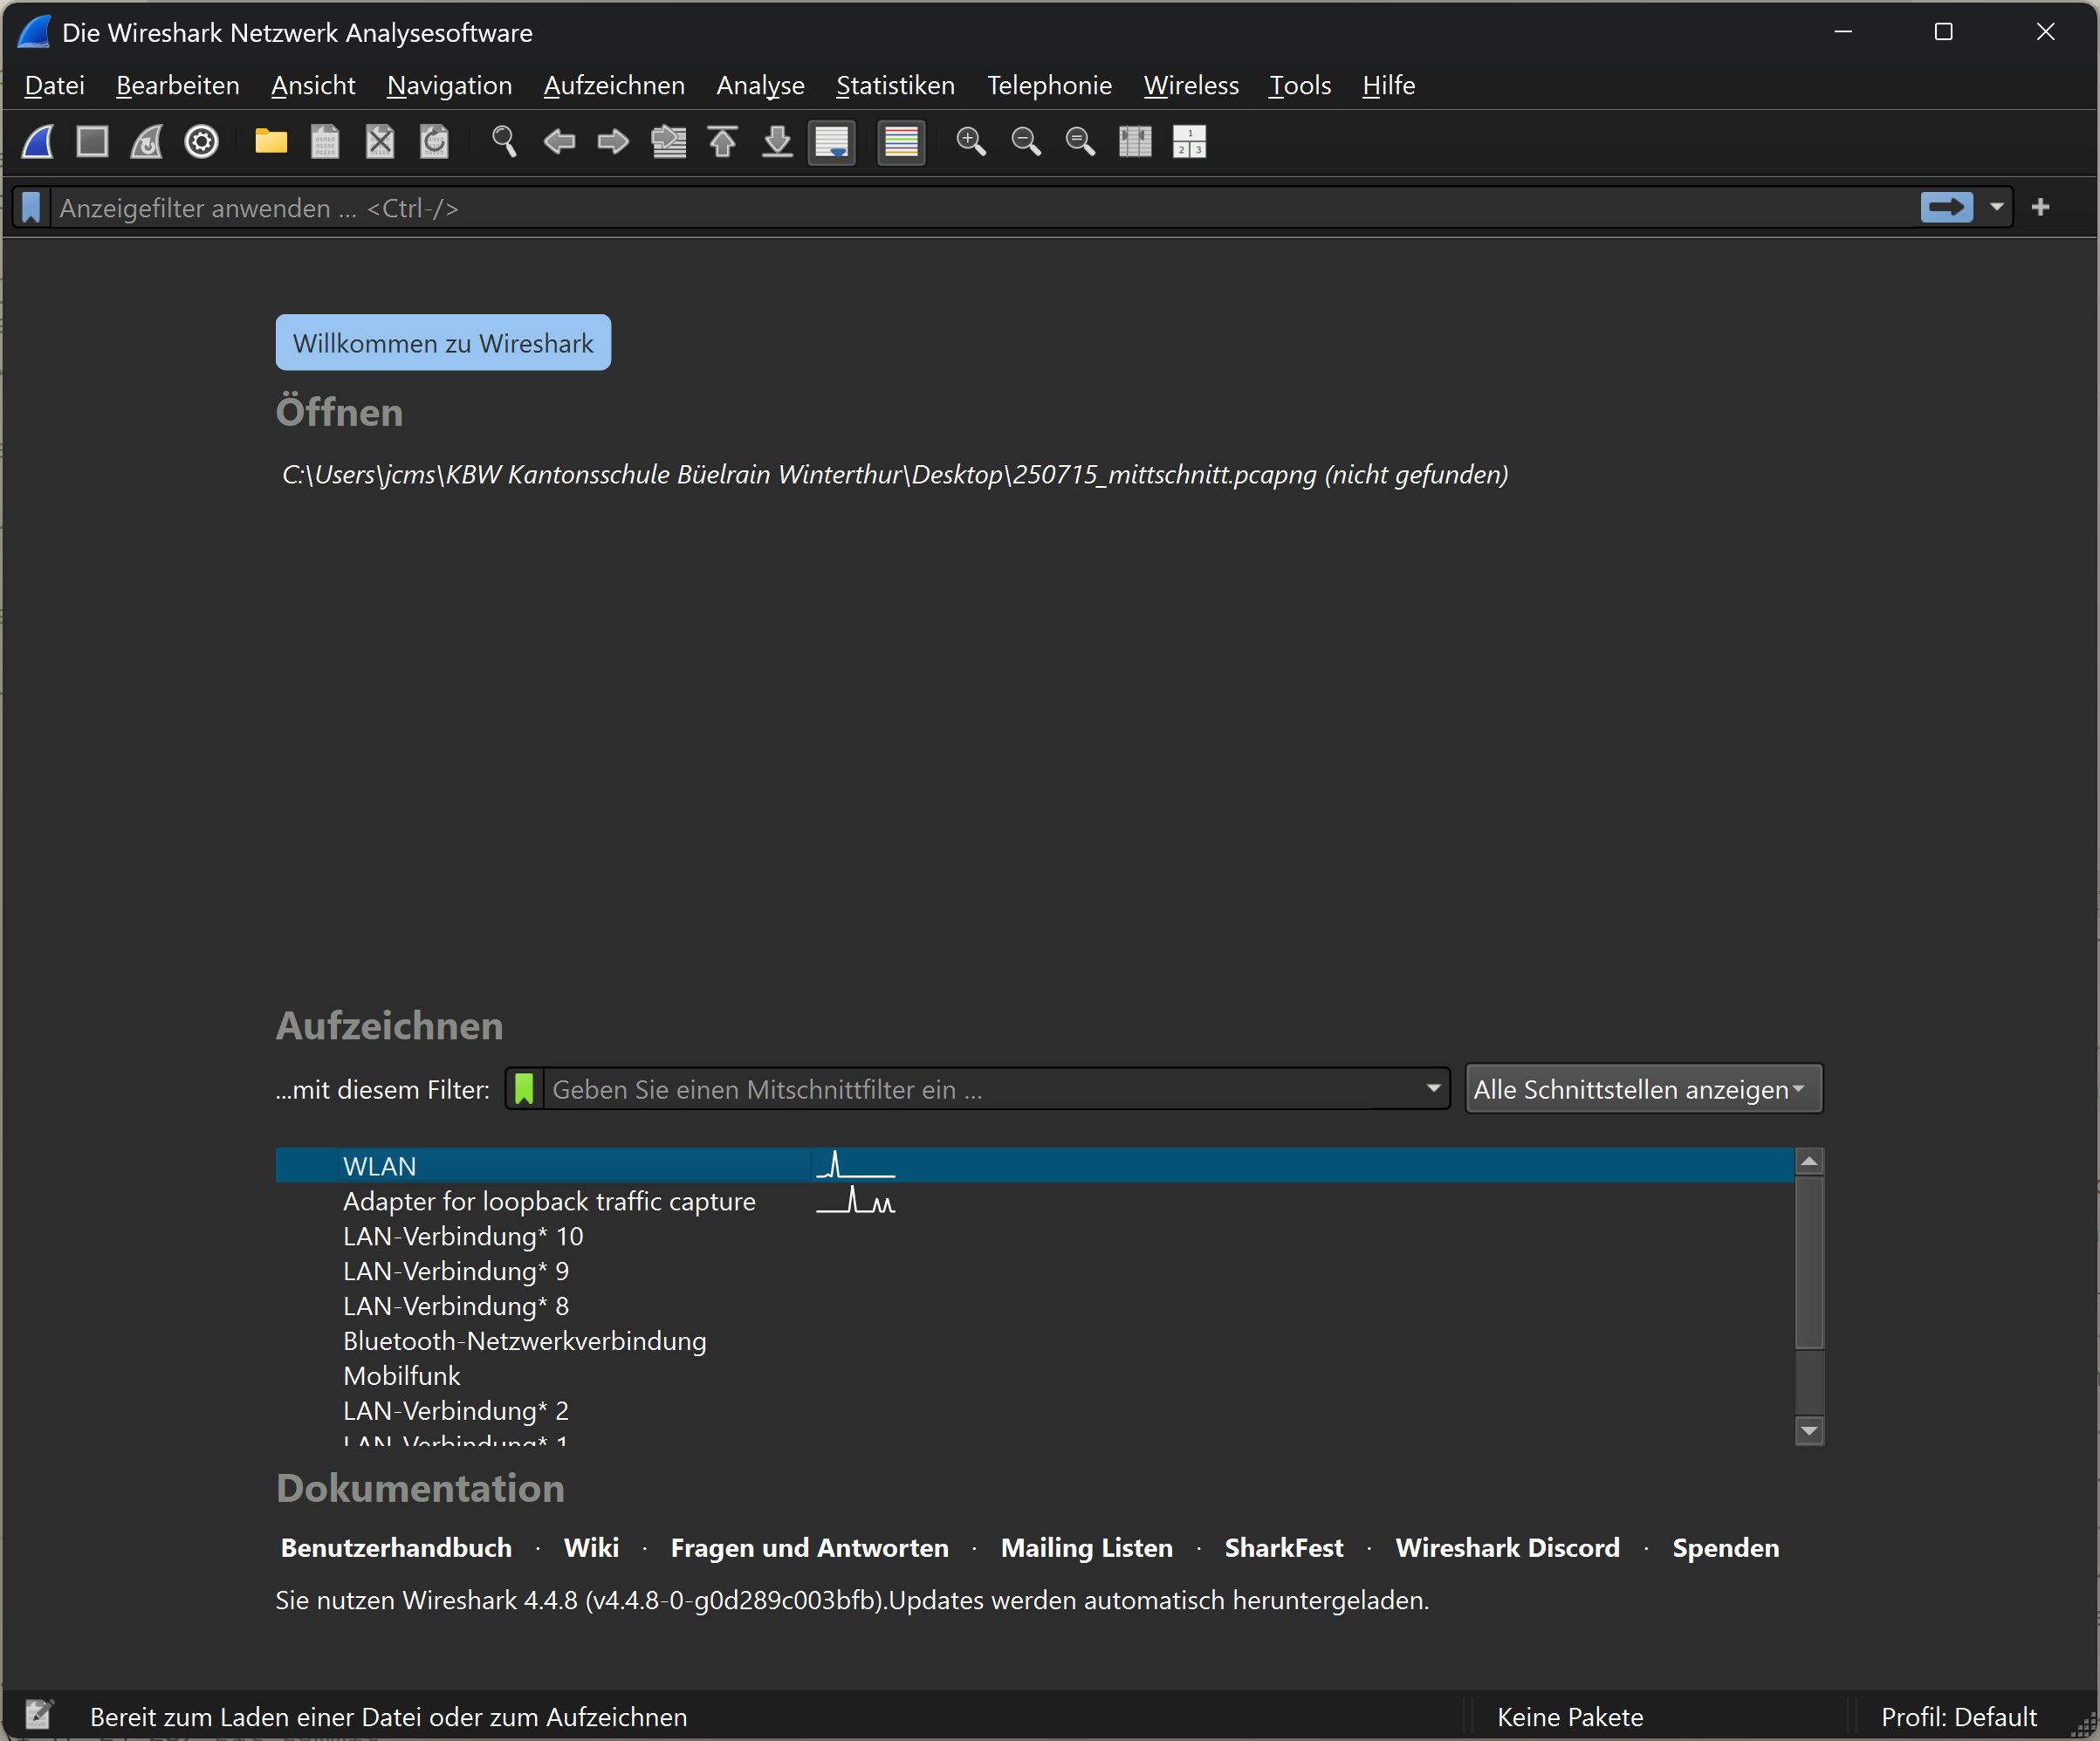
\includegraphics[keepaspectratio]{files/250829/ws_start_window.png}}

}

\caption{Wireshark Startfenster}

\end{figure}%

Unter dem Titel ``Aufzeichnen'' kann der gewünschte Netzwerkadapter
ausgewählt und die Aufzeichnung gestartet werden. Die erfassten Pakete
werden in Echtzeit angezeigt und können später analysiert werden. In der
Schule wird die Verbindung zum Internet per WLAN hergestellt.
Entsprechend ist der WLAN-Adapter auszuwählen. Sobald der entsprechende
Adapter ausgewählt ist, kann die Aufzeichnung gestartet werden.
Gestartet wird die Aufzeichnung durch einen Klick auf das blaue
Haifischflossen-Symbol in der Symbolleiste. Die Aufzeichnung startet
umgehend. Angehalten wird die Aufzeichnung mit einem Klick auf das rote
Quadrat-Symbol in der Symbolleiste. Die Aufzeichnung kann entweder über
das Menü Datei \textgreater{} Speichern, durch einen Klick auf das
Dateisymbol oder durch die Tastenkombination \texttt{Strg\ +\ S}
gespeichert werden.

\section{Beobachten der DNS-Anfragen}\label{beobachten-der-dns-anfragen}

\subsection{Filtern der Aufzeichnung}\label{filtern-der-aufzeichnung}

Um die DNS-Anfragen zu beobachten, wird bei laufender Wireshark
Aufzeichnung eine beliebige Website aufgerufen. Dadurch werden die
entsprechenden DNS-Anfragen erfasst und können in Wireshark analysiert
werden. Nach dem Aufruf der Website kann die Aufzeichnung angehalten und
die erfassten Pakete analysiert werden (wenn die Aufzeichnung
weiterläuft, bewegen sich die Pakete im Anzeigefenster ständig weiter).

Damit die relevanten Datenpakete angezeigt werden, kann der
aufgezeichnete Datenverkehr gefiltert werden. Der Filter wird in der
Eingabefeld für ``Anzeigefilter'' eingegeben.

\begin{figure}[H]

{\centering \pandocbounded{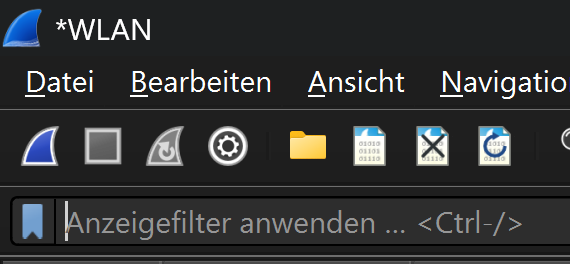
\includegraphics[keepaspectratio]{files/250829/ws_anzeigefilter.png}}

}

\caption{Wireshark Anzeigefilter}

\end{figure}%

Der entsprechende Filter für DNS-Anfragen zu einer gegebenen Website
lautet

\begin{Shaded}
\begin{Highlighting}[numbers=left,,]
\NormalTok{dns.qry.name == "www.example.com"}
\end{Highlighting}
\end{Shaded}

Der angewendete Filterbefehl ist relativ einfach nachzuvollziehen. An
erster Stelle steht hier das Protokoll, nach dem gefiltert wird. Weil
nach den DNS-Anfragen gefiltert wird, ist das hier \texttt{dns}.
\texttt{dns} alleine wäre bereits ein gültiger Filter. Allerdings werden
dann alle DNS-Pakete angezeigt. Der Filter wird daher zu
\texttt{dns.qry.name} ergänzt Dabei steht \texttt{qry} als Abkürzung für
query - Anfrage. Die Ergänzung \texttt{name} steht für den Domain Name,
der Abgefragt wird. \texttt{==} ist die logische Verknüpfung, nach der
gefiltert wird und bedeutet hier ``ist gleich''. Zwischen den
Anführungszeichen steht der String, nach dem gesucht wird.\\
Sofern die Seite während der Aufzeichnung genau einmal aufgerufen wurde,
wird der Filter zwei Pakete anzeigen: eine DNS-Anfrage und eine
DNS-Antwort.

\begin{figure}[H]

{\centering \pandocbounded{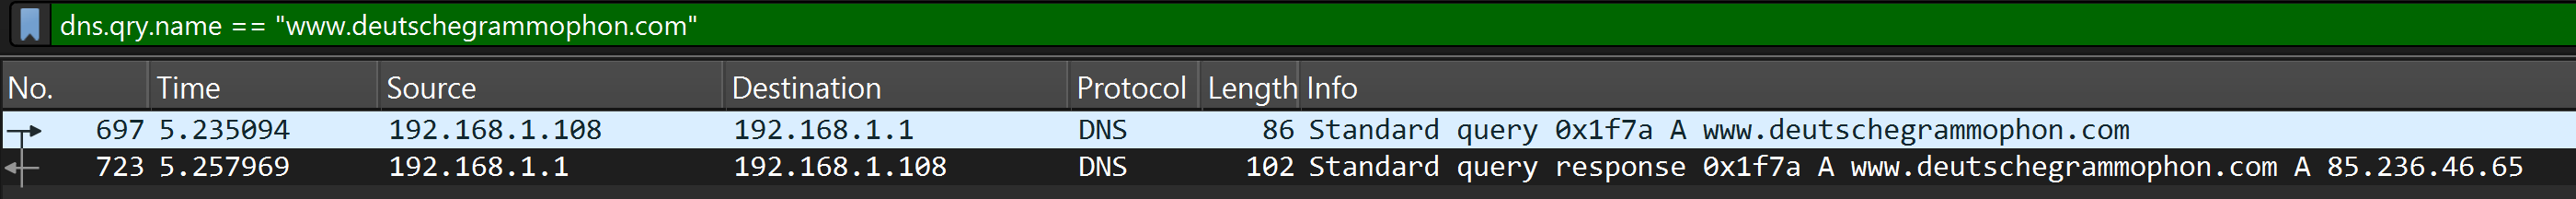
\includegraphics[keepaspectratio]{files/250829/ws_dns_query.png}}

}

\caption{Gefilterte Wireshark-Pakete}

\end{figure}%

Das Bild zeigt als erstes Paket die DNS-Anfrage für
www.deutschegrammaphon.com und als zweites Paket die entsprechende
Antwort.

\subsection{Analyse der gefilterten
Pakete}\label{analyse-der-gefilterten-pakete}

Für eine genaue Analyse der Kommunikation kann ein einzelnes Paket durch
anklicken ausgewählt werden. Dadurch wird das Paket im unteren Bereich
von Wireshark detailliert angezeigt und kann genauer untersucht werden.

\begin{figure}[H]

{\centering \pandocbounded{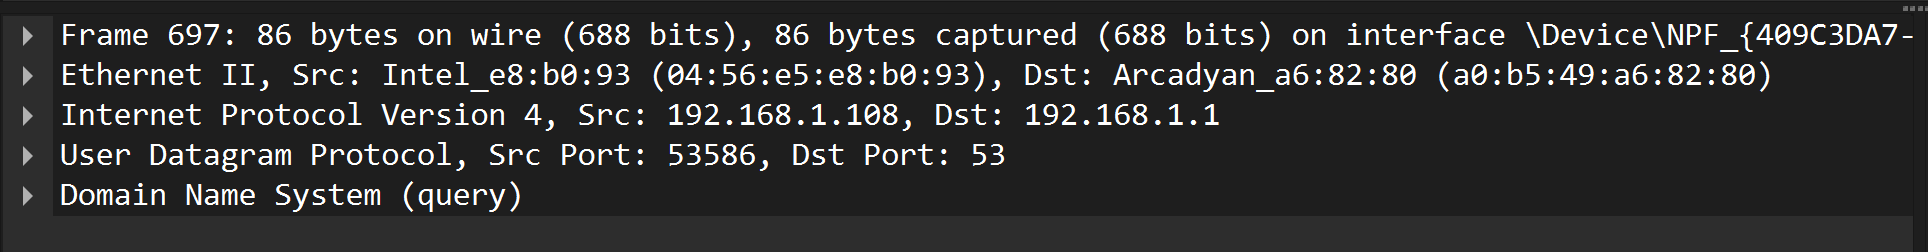
\includegraphics[keepaspectratio]{files/250829/ws_selected_package.png}}

}

\caption{Inhalt des Ausgewählten Pakets}

\end{figure}%

Dass es sich hier im Bild um die Details des ausgewählten Paketes
handelt, ist an der übereinstimmenden Paketnummer zu erkennen. Die
Zeilen in der Detailansicht entsprechen den einzelnen
Protokoll-Header-Feldern des ausgewählten Paketes. Das bildet auch das
TCP/IP Schichtenmodell ab.

Die Detailansicht kann durch einen Klick auf die Dreiecke am Anfang der
einzelnen Protokoll-Header-Felder erweitert werden. Dadurch werden
weitere Informationen zu den jeweiligen Feldern angezeigt. Hier werden
jedoch nur die Zusammenfassungen der Header-Felder erläutert.

Im Beispiel wird als erstes der Inhalt des Headers des Internetlayers
erläutert.

\begin{Shaded}
\begin{Highlighting}[numbers=left,,]

\NormalTok{Internet Protocol Version 4, Src: 192.168.1.108, Dst: 192.168.1.1}
\end{Highlighting}
\end{Shaded}

In der Zusammenfassung werden die Quell- und Ziel-Adressen des IP-Pakets
angezeigt. Im vorliegenden Fall sind das jeweils die Privaten
IP-Adressen 192.168.1.108 und 192.168.1.1. 192.168.1.108 ist die
Quell-Adresse, erkennbar an der Abkürzung ``Src'' und 192.168.1.1 die
Ziel-Adresse, erkennbar an der Abkürzung ``Dst''. Beide Geräte befinden
sich damit im gleichen LAN. Der Rechner mit der IP-Adresse 192.168.1.1
ist der Router. Dieses Gerät stellt die Internetverbindung her und kann
DNS-Anfragen aus seinem Cache beantworten.

Im Header für das User Datagram Protocol (UDP) werden die Quell- und
Ziel-Ports angezeigt.

\begin{Shaded}
\begin{Highlighting}[numbers=left,,]
\NormalTok{User Datagram Protocol, Src Port: 53586, Dst Port: 53}
\end{Highlighting}
\end{Shaded}

Der Quellport wurde mit 53586 automatisch und weit oberhalb der sog.
``Well-Known Ports'' (0-1023) gewählt. Die ``Well-Known Ports'' sind
Ports, die von bestimmten Anwendungen oder Diensten standardmässig
verwendet werden. Entsprechend wurde der Zielport auf 53 gewählt, da
dies der standardmässige Port für DNS-Anfragen ist. Eine Liste der
``Well-Known Ports'' findet sich in der offiziellen IANA-Portdatenbank.
Der Quellport ermöglicht es dem Zielsystem, die Antwort an den korrekten
Absender zurückzusenden. NAT-Geräte (vgl.
\hyperref[network-address-translation-nat]{Abschnitt Network Address
Translation (NAT)}) nutzen diese Port-Informationen zusätzlich für die
Zuordnung zwischen privaten und öffentlichen Adressen.

Der zuunterst dargestellte Layer in der Detailansicht, beinhaltet die
eigentliche Anfrage für die Übersetzung des Domainnamens in eine
IP-Adresse.

\begin{Shaded}
\begin{Highlighting}[numbers=left,,]
\NormalTok{Domain Name System (query)}
\NormalTok{    Transaction ID: 0x1f7a}
\NormalTok{    Flags: 0x0100 Standard query}
\NormalTok{    Questions: 1}
\NormalTok{    Answer RRs: 0}
\NormalTok{    Authority RRs: 0}
\NormalTok{    Additional RRs: 0}
\NormalTok{    Queries}
\NormalTok{        www.deutschegrammophon.com: type A, class IN}
\NormalTok{    [Response In: 723]}
\end{Highlighting}
\end{Shaded}

Aus diesem Grund wird dieser Teil der Analyse hier auch aufgefaltet
dargestellt.\\
Unter dem Stichwort \texttt{Queries} wird die gesuchte Adresse
\texttt{www.deutschegrammophon.com} angezeigt. Das Stichwort
\texttt{type\ A} zeigt an, dass es sich hier um eine Anfrage nach einer
IPv4-Adresse handelt. IPv4-Adressen werden mit \texttt{A} bezeichnet,
IPv6 mit \texttt{AAAA}. Das letzte Element in dieser Zeile ist die
Klasse der Anfrage, in diesem Fall \texttt{IN} für das Internet. Obwohl
heute fast ausschliesslich das Internet als Netzwerktyp verwendet wird,
ist das Feld für die Klasse (IN) aus historischen Gründen weiterhin Teil
jeder DNS-Anfrage.

Der entsprechende Inhalt der Antwort sieht folgendermassen aus:

\begin{Shaded}
\begin{Highlighting}[numbers=left,,]
\NormalTok{Domain Name System (response)}
\NormalTok{    Transaction ID: 0x1f7a}
\NormalTok{    Flags: 0x8180 Standard query response, No error}
\NormalTok{    Questions: 1}
\NormalTok{    Answer RRs: 1}
\NormalTok{    Authority RRs: 0}
\NormalTok{    Additional RRs: 0}
\NormalTok{    Queries}
\NormalTok{        www.deutschegrammophon.com: type A, class IN}
\NormalTok{    Answers}
\NormalTok{        www.deutschegrammophon.com: type A, class IN, addr 85.236.46.65}
\end{Highlighting}
\end{Shaded}

Das Paket wiederholt die Frage und liefert die Antwort des DNS-Servers.
Der Domainname \texttt{www.deutschegrammophon.com} ist mit der
IPv4-Adresse \texttt{85.236.46.65} verknüpft.

Damit kann die Verbindung zur Website
\texttt{www.deutschegrammophon.com} hergestellt werden.

\section{Beobachtung des
Verbindungsaufbaus}\label{beobachtung-des-verbindungsaufbaus}

Der Verbindungsaufbau zwischen Client (lokaler Rechner) und Server
(Rechner im Internet) erfolgt in mehreren Schritten, die im sogenannten
``Three-Way Handshake'' zusammengefasst werden. Dieser Prozess stellt
sicher, dass beide Seiten bereit sind, Daten zu senden und zu empfangen.
Die folgende Abbildung zeigt eine schematische Darstellung des
``Three-Way Handshake''.

\begin{figure}[H]

{\centering \pandocbounded{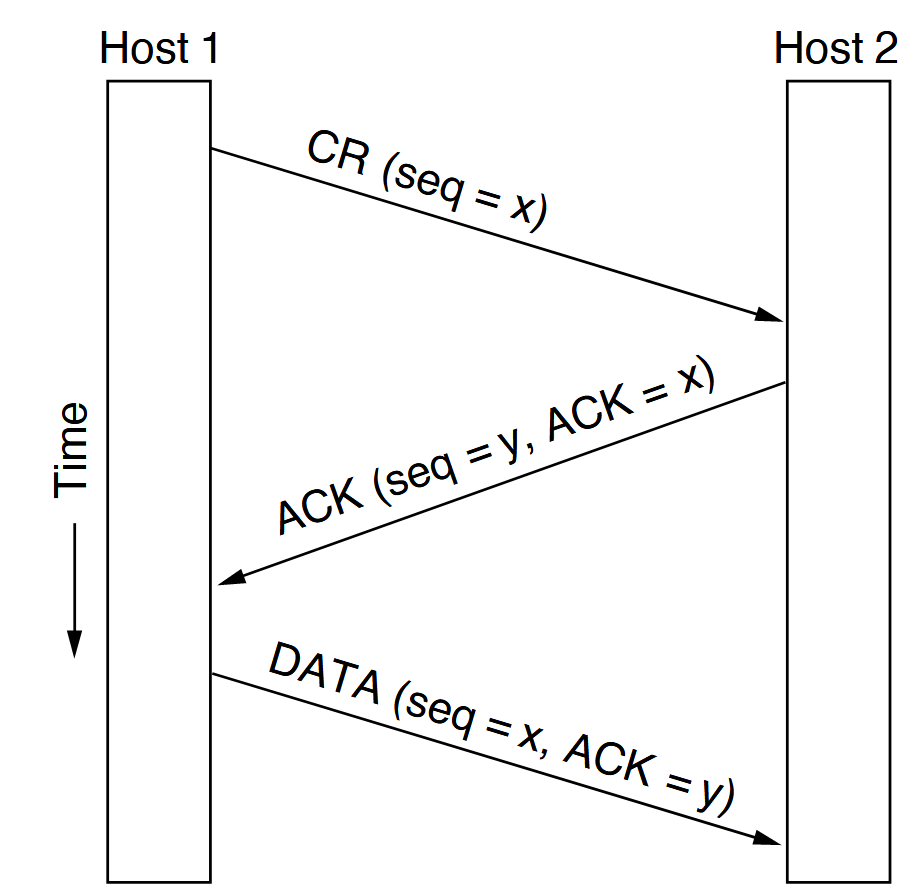
\includegraphics[keepaspectratio]{files/250829/schema_three-way-handshake.png}}

}

\caption{Schema Three-Way Handshake}

\end{figure}%

Der Client sendet ein SYN-Paket an den Server, um eine Verbindung
anzufordern. Dieser atwortet mit einem SYN-ACK-Paket. Das heisst, er
bestätigt die Anfrage mit einem ACK und fragt seinerseits mit einem SYN
nach, ob der Client (immer noch) bereit ist, die Verbindung aufzubauen.
Damit klar ist, dass sich das ACK im SYN-ACK-Paket auf das ursprüngliche
SYN-Paket bezieht, werden die einzelnen Pakete mit einer Sequenznummer
(Sequence Number) versehen. Das ACK gibt die Sequenznummer des
SYN-Paketes plus eins zurück.

Dieser Vorgang kann mit Wireshark beobachtet werden. Dafür braucht es
einen kombinierten Wireshark Anzeigefilter. Als Beispiel wird der
Verbindungsaufbau zwischen dem lokalen Rechner und der Website von
www.deutschegrammophon.com betrachtet. Der erste Teil des Filters soll
nur jene Pakete anzeigen, welche mit der IP-Adresse des Servers von
www.deutschegrammophon.com (85.236.46.65) kommunizieren. Dieser Filter
lautet

\begin{Shaded}
\begin{Highlighting}[numbers=left,,]
\NormalTok{ip.addr == 85.236.46.65}
\end{Highlighting}
\end{Shaded}

Dieser Filter alleine zeigt jedoch noch zu viele Pakete an.

\begin{figure}[H]

{\centering \pandocbounded{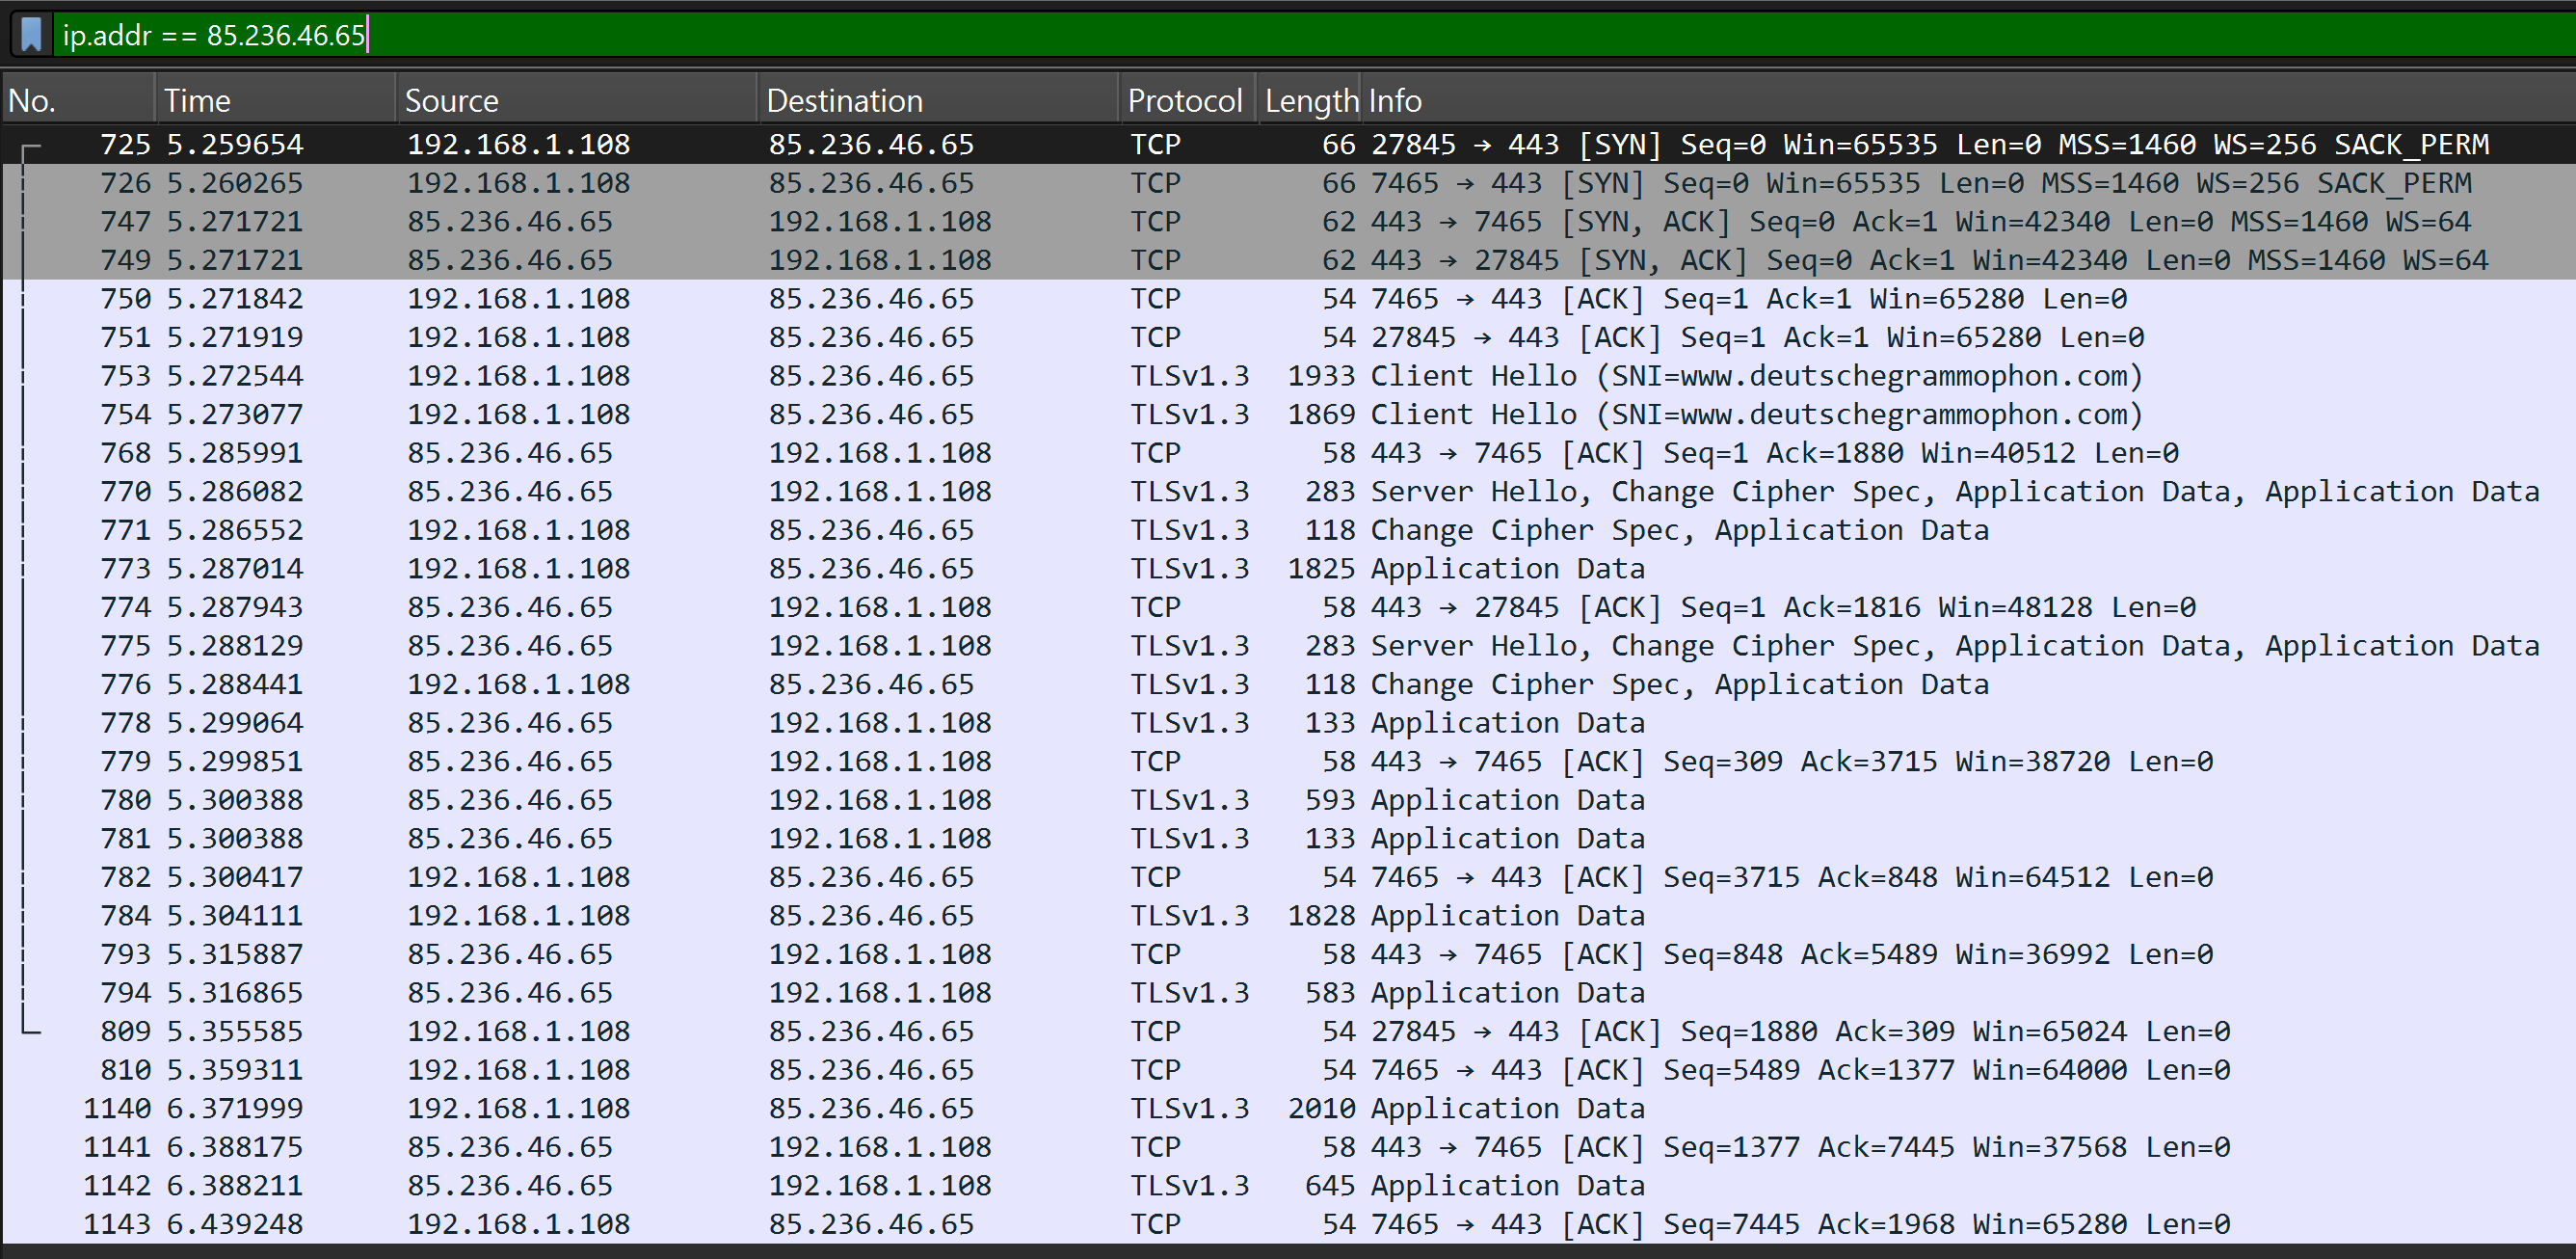
\includegraphics[keepaspectratio]{files/250829/ws_ip-addr-Filter.png}}

}

\caption{ip.addr Filter}

\end{figure}%

Um die Resultate weiter einzuschränken sollen nur jene Pakete angezeigt
werden, welche entweder das SYN-Flag oder das ACK-Flag (oder beides)
gesetzt haben. Dies kann mit folgendem Filter erreicht werden:

\begin{Shaded}
\begin{Highlighting}[numbers=left,,]
\NormalTok{ip.addr == 85.236.46.65 and (tcp.flags.syn == 1 or tcp.flags.ack == 1 )}
\end{Highlighting}
\end{Shaded}

Das sind allerdings immer noch zu viele Pakete. Daher sollen nur jene
Pakete angezeigt werden, welche die Antworten auf eine SYN-Anfrage sind.
Das kann erreicht werden, in dem ein Paket mit dem SYN-Flag mit der
rechten Maustaste angeklickt wird und die Option ``Follow''
\textgreater{} ``TCP Stream'' ausgewählt wird. Dadurch wird der gesamte
TCP-Stream, in dem dieses Paket steht, (die aufeinanderfolgenden Pakete)
angezeigt. Der Filter wird automatisch angepasst.

Das folgende Listing zeigt den ganzen Filterbefehl für die Anzeige der
Pakete, die zu diesem TCP-Stream gehören:

\begin{Shaded}
\begin{Highlighting}[numbers=left,,]
\NormalTok{ip.addr == 85.236.46.65 and (tcp.flags.syn == 1 or tcp.flags.ack == 1) and !(tcp.stream eq 8)}
\end{Highlighting}
\end{Shaded}

\begin{figure}[H]

{\centering \pandocbounded{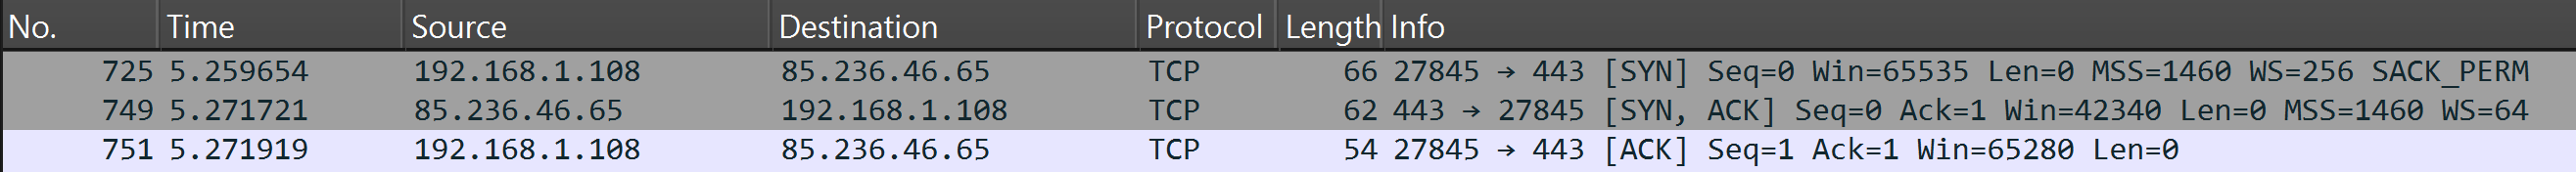
\includegraphics[keepaspectratio]{files/250829/ws_three-way-handshake.png}}

}

\caption{Three-Way Handshake Pakete}

\end{figure}%

Dass die Pakte die Kommunikationsfolge des Three-Way Handshakes zeigen,
ist an den gesetzten Flags zu erkennen. Im ersten Schritt sendet der
Client ein SYN-Paket, worauf der Server mit einem SYN-ACK-Paket
antwortet. Der Client bestätigt dies mit einem ACK-Paket. Diese drei
Schritte sind im Wireshark-Filter sichtbar. Gut zu erkennen sind die
jeweiligen Portnummern, die in den TCP-Paketen verwendet werden.

Anschliessend an diesen ``Three-Way Handshake'' kann der Client mit dem
Server kommunizieren.

\chapter{Python Sockets: Ein Einfaches Client-Server
Beispiel}\label{python-sockets-ein-einfaches-client-server-beispiel}

In diesem Abschnitt untersuchen wir, wie man eine einfache
Client-Server-Anwendung mit Python-Sockets erstellt. Dieses Beispiel
wird die grundlegenden Konzepte der Socket-Programmierung demonstrieren,
einschliesslich der Herstellung einer Verbindung sowie des Sendens und
Empfangens von Daten.

\begin{tcolorbox}[enhanced jigsaw, arc=.35mm, bottomrule=.15mm, bottomtitle=1mm, breakable, colback=white, colbacktitle=quarto-callout-note-color!10!white, colframe=quarto-callout-note-color-frame, coltitle=black, left=2mm, leftrule=.75mm, opacityback=0, opacitybacktitle=0.6, rightrule=.15mm, title=\textcolor{quarto-callout-note-color}{\faInfo}\hspace{0.5em}{Network Socket}, titlerule=0mm, toprule=.15mm, toptitle=1mm]

Ein Netzwerk-Socket ist ein Endpunkt innerhalb eines Hosts, der zum
Senden und Empfangen von Daten über ein Netzwerk verwendet wird.

\end{tcolorbox}

\section{Struktur der Verbindung}\label{struktur-der-verbindung}

Das Beispiel besteht aus einem Server, der auf eingehende Verbindungen
wartet, und einem Client, der sich mit dem Server verbindet. Wir werden
die Kommunikation als einfachen Chatdienst modellieren.

\section{Server Code}\label{server-code}

Sie benötigen keine virtuelle Umgebung. Das Beispiel verwendet nur die
Python-Standardbibliothek.\\
Unten ist das funktionierende Codebeispiel für den Socket-Server:

\begin{Shaded}
\begin{Highlighting}[numbers=left,,]
\CommentTok{\# socket\_server.py}

\ImportTok{import}\NormalTok{ socket}

\KeywordTok{def}\NormalTok{ server\_program():}
    \CommentTok{\# define host name and port}
\NormalTok{    host }\OperatorTok{=} \StringTok{\textquotesingle{}localhost\textquotesingle{}}    \CommentTok{\# for communication on the local machine}
\NormalTok{    port }\OperatorTok{=} \DecValTok{5000}           \CommentTok{\# use a port number above 1024}
    
    \CommentTok{\# create socket}
\NormalTok{    server\_socket }\OperatorTok{=}\NormalTok{ socket.socket()}
    
    \CommentTok{\# bind the socket to the host and port}
\NormalTok{    server\_socket.bind((host, port))}
    
    \CommentTok{\# set the server to listen for connections}
\NormalTok{    server\_socket.listen(}\DecValTok{2}\NormalTok{) }\CommentTok{\# start listening }
                            \CommentTok{\# with a backlog of 2 }
                            \CommentTok{\# (max queued connections)}
    
    \CommentTok{\# accept new connection from client}
\NormalTok{    conn, address }\OperatorTok{=}\NormalTok{ server\_socket.accept()}
    \BuiltInTok{print}\NormalTok{(}\StringTok{"Connection from: "} \OperatorTok{+} \BuiltInTok{str}\NormalTok{(address))}
    
    \ControlFlowTok{while} \VariableTok{True}\NormalTok{:}
        \CommentTok{\# receive up to 1024 bytes per call}
\NormalTok{        data }\OperatorTok{=}\NormalTok{ conn.recv(}\DecValTok{1024}\NormalTok{).decode()}
        \ControlFlowTok{if} \KeywordTok{not}\NormalTok{ data:}
            \CommentTok{\# if no data is received, break}
            \ControlFlowTok{break}
        \BuiltInTok{print}\NormalTok{(}\StringTok{"Received from connected client: "} \OperatorTok{+} \BuiltInTok{str}\NormalTok{(data))}
        \CommentTok{\# prompt the user to enter a message}
\NormalTok{        data }\OperatorTok{=} \BuiltInTok{input}\NormalTok{(}\StringTok{\textquotesingle{} {-}\textgreater{} \textquotesingle{}}\NormalTok{)}
        \CommentTok{\# send data to the client as bytes}
\NormalTok{        conn.send(data.encode())}
        
    \CommentTok{\# close the connection}
\NormalTok{    conn.close()}
    
\ControlFlowTok{if} \VariableTok{\_\_name\_\_} \OperatorTok{==} \StringTok{\textquotesingle{}\_\_main\_\_\textquotesingle{}}\NormalTok{:}
\NormalTok{    server\_program()}
\end{Highlighting}
\end{Shaded}

Um das Skript direkt auszuführen, öffnen Sie ein Terminal im
Verzeichnis, in dem sich das Skript befindet, und führen Sie den
folgenden Befehl aus:

\begin{Shaded}
\begin{Highlighting}[numbers=left,,]
\ExtensionTok{python}\NormalTok{ socket\_server.py}
\end{Highlighting}
\end{Shaded}

Was geschieht, wenn das Skript ausgeführt wird, wird in den folgenden
Abschnitten erläutert.

Der Code besteht aus zwei Hauptteilen: der Funktion
\texttt{server\_program} und dem Block
\texttt{if\ \_\_name\_\_\ ==\ \textquotesingle{}\_\_main\_\_\textquotesingle{}}.
Die Funktion \texttt{server\_program} enthält die Hauptlogik für den
Server, während der \texttt{if}-Block verwendet wird, um den Servercode
auszuführen, wenn das Skript direkt ausgeführt wird.

Wenn Sie das Skript ausführen, importiert Python zuerst das
\texttt{socket}-Modul.

\begin{Shaded}
\begin{Highlighting}[numbers=left,,]
\ImportTok{import}\NormalTok{ socket}
\end{Highlighting}
\end{Shaded}

Als nächstes wird die Funktion \texttt{server\_program} aufgerufen.
Innerhalb dieser Funktion wird als erstes die Hostadresse und der
Portnummer definiert. \texttt{localhost} ist eine spezielle Adresse, die
auf die lokale Maschine verweist. \texttt{localhost} entspricht der
IPv4-Adresse \texttt{127.0.0.1}. Das bedeutet, dass der Server nur
Verbindungen von Clients akzeptiert, die auf derselben Maschine
ausgeführt werden. Dies ist eine Simulation eines Netzwerks.

\begin{Shaded}
\begin{Highlighting}[numbers=left,,]
\KeywordTok{def}\NormalTok{ server\_program():}
    \CommentTok{\# define host name and port}
\NormalTok{    host }\OperatorTok{=} \StringTok{\textquotesingle{}localhost\textquotesingle{}}    \CommentTok{\# for communication on the local machine}
\NormalTok{    port }\OperatorTok{=} \DecValTok{5000}           \CommentTok{\# use a port number above 1024}
\end{Highlighting}
\end{Shaded}

Im nächsten Code-Snippet wird der \texttt{server\_socket} mit der
Funktion \texttt{socket.socket()} erstellt, die ein neues Socket-Objekt
erzeugt.

\begin{Shaded}
\begin{Highlighting}[numbers=left,,]
\NormalTok{server\_socket }\OperatorTok{=}\NormalTok{ socket.socket()}
\end{Highlighting}
\end{Shaded}

Dieses Socket wird verwendet, um auf eingehende Verbindungen von Clients
zu hören. Damit die Verbindung funktioniert, muss der
\texttt{server\_socket} mit der Host- und Portnummer über die
\texttt{bind()}-Methode verbunden werden.

\begin{Shaded}
\begin{Highlighting}[numbers=left,,]
\NormalTok{server\_socket.bind((host, port))}
\end{Highlighting}
\end{Shaded}

Als nächstes wird der Server so eingestellt, dass er mit der
\texttt{listen()}-Methode auf eingehende Verbindungen wartet.

\begin{Shaded}
\begin{Highlighting}[numbers=left,,]
\NormalTok{server\_socket.listen(}\DecValTok{2}\NormalTok{) }\CommentTok{\# start listening }
                        \CommentTok{\# with a backlog of 2 }
                        \CommentTok{\# (max queued connections)}
\end{Highlighting}
\end{Shaded}

Der Server erstellt ein backlog von 2 ausstehenden Verbindungen. Der
Code akzeptiert jedoch genau eine Client-Verbindung (accept() wird
einmal aufgerufen). Um mehrere Clients zu verarbeiten, rufen Sie
accept() in einer Schleife auf und verwenden Sie Threads oder asyncio.
Dieses Limit wird festgelegt, um zu verhindern, dass der Server von zu
vielen Verbindungen auf einmal überwältigt wird. Die
\texttt{accept()}-Methode wird verwendet, um eine neue Verbindung von
einem Client zu akzeptieren. Diese Methode gibt ein Tupel mit zwei
Elementen zurück: \texttt{conn}, ein neues Socket-Objekt für die
Kommunikation mit dem Client, und \texttt{address}, die Adresse des
Clients. Der nächste Abschnitt zeigt, wie eine Nachricht ausgegeben
wird, um die Adresse des verbundenen Clients anzuzeigen.

\begin{Shaded}
\begin{Highlighting}[numbers=left,,]
\NormalTok{conn, address }\OperatorTok{=}\NormalTok{ server\_socket.accept()}
\BuiltInTok{print}\NormalTok{(}\StringTok{"Connection from: "} \OperatorTok{+} \BuiltInTok{str}\NormalTok{(address))}
\end{Highlighting}
\end{Shaded}

Die while-Schleife ermöglicht es dem Server, auf Daten vom Client zu
warten. Die \texttt{recv()}-Methode wird verwendet, um Daten vom Client
zu empfangen. Jeder \texttt{recv()}-Aufruf liest bis zu 1024 Bytes;
zusätzliche Daten bleiben im Puffer und können durch nachfolgende
Aufrufe gelesen werden. Wenn keine Daten empfangen werden, bricht der
Server die Schleife ab und schliesst die Verbindung.

\begin{Shaded}
\begin{Highlighting}[numbers=left,,]
\ControlFlowTok{while} \VariableTok{True}\NormalTok{:}
        \CommentTok{\# receive up to 1024 bytes per call}
\NormalTok{        data }\OperatorTok{=}\NormalTok{ conn.recv(}\DecValTok{1024}\NormalTok{).decode()}
        \ControlFlowTok{if} \KeywordTok{not}\NormalTok{ data:}
            \CommentTok{\# if no data is received, break}
            \ControlFlowTok{break}
        
\end{Highlighting}
\end{Shaded}

Wenn der Server Daten empfängt, gibt er die Daten in der Konsole aus und
fordert den Benutzer auf, eine Antwort einzugeben. Die Antwort wird mit
der \texttt{send()}-Methode an den Client zurückgesendet.

\begin{Shaded}
\begin{Highlighting}[numbers=left,,]
\BuiltInTok{print}\NormalTok{(}\StringTok{"Received from connected client: "} \OperatorTok{+} \BuiltInTok{str}\NormalTok{(data))}
        \CommentTok{\# prompt the user to enter a message}
\NormalTok{        data }\OperatorTok{=} \BuiltInTok{input}\NormalTok{(}\StringTok{\textquotesingle{} {-}\textgreater{} \textquotesingle{}}\NormalTok{)}
        \CommentTok{\# send data to the client as bytes}
\NormalTok{        conn.send(data.encode())}
\end{Highlighting}
\end{Shaded}

\section{Client Code}\label{client-code}

Unten ist der funktionierende Code des Client-Beispiels:

\begin{Shaded}
\begin{Highlighting}[numbers=left,,]
\CommentTok{\# socket\_client.py}

\ImportTok{import}\NormalTok{ socket}

\KeywordTok{def}\NormalTok{ client\_program():}
    \CommentTok{\# define host name and port (of the server to connect to)}
\NormalTok{    host }\OperatorTok{=} \StringTok{\textquotesingle{}localhost\textquotesingle{}}  \CommentTok{\# as both pieces of code are }
                        \CommentTok{\# running on the same machine}
\NormalTok{    port }\OperatorTok{=} \DecValTok{5000}         \CommentTok{\# socket server port number}
    
    \CommentTok{\# create socket}
\NormalTok{    client\_socket }\OperatorTok{=}\NormalTok{ socket.socket()}
    
    \CommentTok{\# connect to the server}
\NormalTok{    client\_socket.}\ExtensionTok{connect}\NormalTok{((host, port))}
    
    \CommentTok{\# prompt the user to enter a message}
\NormalTok{    message }\OperatorTok{=} \BuiltInTok{input}\NormalTok{(}\StringTok{" {-}\textgreater{} "}\NormalTok{)  }\CommentTok{\# take input}
    
    \CommentTok{\# message loop}
    \ControlFlowTok{while}\NormalTok{ message.lower().strip() }\OperatorTok{!=} \StringTok{\textquotesingle{}bye\textquotesingle{}}\NormalTok{:}
        \CommentTok{\# send message to the server as bytes}
\NormalTok{        client\_socket.send(message.encode())}
        
        \CommentTok{\# receive response from the server}
\NormalTok{        data }\OperatorTok{=}\NormalTok{ client\_socket.recv(}\DecValTok{1024}\NormalTok{).decode()}
        
        \BuiltInTok{print}\NormalTok{(}\StringTok{\textquotesingle{}Received from server: \textquotesingle{}} \OperatorTok{+}\NormalTok{ data)}
        
        \CommentTok{\# prompt the user to enter a new message}
\NormalTok{        message }\OperatorTok{=} \BuiltInTok{input}\NormalTok{(}\StringTok{" {-}\textgreater{} "}\NormalTok{)  }\CommentTok{\# take new input}
        
    \CommentTok{\# close the connection}
\NormalTok{    client\_socket.close()}
    
\ControlFlowTok{if} \VariableTok{\_\_name\_\_} \OperatorTok{==} \StringTok{\textquotesingle{}\_\_main\_\_\textquotesingle{}}\NormalTok{:}
\NormalTok{    client\_program()}
\end{Highlighting}
\end{Shaded}

Um dieses Skript auszuführen, befolgen Sie die gleichen Schritte wie für
das Server-Skript. Öffnen Sie ein Terminal im Verzeichnis, in dem sich
das Skript befindet, und führen Sie den folgenden Befehl aus:

\begin{Shaded}
\begin{Highlighting}[numbers=left,,]
\ExtensionTok{python}\NormalTok{ socket\_client.py}
\end{Highlighting}
\end{Shaded}

Starten Sie den Server, bevor Sie den Client starten. Wenn der Server
nicht läuft, wird client\_socket.connect(\ldots) einen
ConnectionRefusedError auslösen.

Wenn Sie das Skript ausführen, importiert Python zuerst das Modul
\texttt{socket}.

Als nächstes wird die Funktion \texttt{client\_program} aufgerufen.
Innerhalb dieser Funktion wird die erste Aktion die Definition der
Hostadresse und der Portnummer. Hier müssen die Hostadresse und die
Portnummer mit denen im Server-Skript übereinstimmen.

Nachdem die Host- und Portinformationen definiert sind, erstellt der
Client ein Socket-Objekt mit der Funktion \texttt{socket.socket()}.
Dieses Socket wird verwendet, um eine Verbindung zum Server
herzustellen. Die Methode \texttt{connect()} wird auf dem Socket-Objekt
aufgerufen, um eine Verbindung zum Server herzustellen.

Sobald die Verbindung hergestellt ist, betritt der Client eine Schleife,
in der er Nachrichten an den Server senden und Antworten empfangen kann.
Der Client fordert den Benutzer auf, eine Nachricht einzugeben, die dann
mit der Methode \texttt{send()} an den Server gesendet wird. Der Client
wartet auch auf eine Antwort vom Server, indem er die Methode
\texttt{recv()} verwendet.

Wenn der Benutzer \texttt{bye} eingibt, verlässt der Client die Schleife
und schliesst die Verbindung zum Server.

\section{Verbindung im LAN}\label{verbindung-im-lan}

Um die beiden Skripte im lokalen Netzwerk (LAN) zu verwenden, muss in
beiden Skripten die IPv4-Adresse des Servers anstelle von
\texttt{localhost} verwendet werden.\\
Die IPv4-Adresse des Servers kann durch Ausführen des folgenden Befehls
im Terminal des Servers ermittelt werden:

\begin{Shaded}
\begin{Highlighting}[numbers=left,,]
\ExtensionTok{C:\textbackslash{}Users\textbackslash{}username}\OperatorTok{\textgreater{}}\NormalTok{ipconfig}
\ExtensionTok{Windows}\NormalTok{ IP Configuration}
\ExtensionTok{...}
\ExtensionTok{Wireless}\NormalTok{ LAN adapter Wi{-}Fi:}
   \ExtensionTok{Connection{-}specific}\NormalTok{ DNS Suffix  . . . :}
   \ExtensionTok{IPv4}\NormalTok{ Address . . . . . . . . . . . . .: 192.168.1.2}
   \ExtensionTok{Subnet}\NormalTok{ Mask . . . . . . . . . . . . . : 255.255.255.255}
   \ExtensionTok{Default}\NormalTok{ Gateway . . . . . . . . . . . : 192.168.1.1}
\ExtensionTok{...}
\end{Highlighting}
\end{Shaded}

Die Ausgabe des Befehls \texttt{ipconfig} zeigt alle Netzwerkadapter des
entsprechenden Computers an. Die dargestellte Ausgabe hier im Beispiel
wurde gekürzt.\\
Die IPv4-Adresse des Servers ist in diesem Fall \texttt{192.168.1.2}.

Diese ist die Adresse, welche in beiden Skripten anstelle von
\texttt{localhost} verwendet werden muss. Dann kann innerhalb des
lokalen Netzwerks eine Verbindung hergestellt werden.

\section{Fazit}\label{fazit}

Die vorgestellten Codebeispiele veranschaulichen, wie Pythons
integriertes Socket-Modul (Standardbibliothek) eine unkomplizierte
Implementierung von netzwerkbasierten Anwendungen ermöglicht, ohne
externe Abhängigkeiten zu erfordern. Der Fokus des Tutorials auf die
Kommunikation über localhost bietet eine sichere, kontrollierte Umgebung
für Experimente und Lernen, während der bidirektionale
Nachrichtenaustausch reale Kommunikationsmuster demonstriert, die in
Produktionssystemen zu finden sind.

Zu den wichtigsten Erfolgen dieser Implementierung gehören:

\begin{itemize}
\tightlist
\item
  Erfolgreiche Herstellung von TCP-Socket-Verbindungen zwischen
  separaten Prozessen
\item
  Implementierung einer nachrichtenbasierten Kommunikation mit
  ordnungsgemässer Kodierung/Dekodierung
\item
  Demonstration des Verbindungslebenszyklusmanagements von der
  Herstellung bis zur Beendigung
\item
  Erstellung einer einfachen Befehlszeilenschnittstelle für sowohl
  Server- als auch Clientanwendungen
\end{itemize}

Das Wissen, das aus diesem Tutorial gewonnen wurde, dient als solide
Grundlage für die Entwicklung anspruchsvollerer netzwerkbasierter
Anwendungen. Zukünftige Verbesserungen könnten die Implementierung von
Multithreading für die gleichzeitige Verarbeitung mehrerer Clients, die
Hinzufügung von Fehlerbehandlungs- und Wiederverbindungslogik oder die
Erweiterung des Kommunikationsprotokolls zur Unterstützung
strukturierter Datenformate umfassen.

\part{Datenbanken}

\chapter{Einführung in Datenbanken}\label{einfuxfchrung-in-datenbanken}

Die Einführung in Datenbanken basiert auf dem Einführungskapitel aus dem
Buch Abraham Silberschatz, Henry F. Korth und S. Sudarshan; Database
system concepts; Seventh edition; New York 2020.

\section{Einführung}\label{einfuxfchrung}

Die bisher besprochenen Datenstrukturen Dictionary, Stack, Queue und
Binary Search Tree dienen der Bearbeitung von Daten im Arbeitsspeicher.
Sie sind daher auf einen beschränkten Umfang von Datensätzen ausgelegt.
Ausserdem dienen sie nicht der permanenten Ablage von Daten.

Im Gegensatz dazu dienen Datenbanken der dauerhaften Ablage grosser
Datensätze. Darüber hinaus sollen sie die effiziente Verfügbarkeit und
die Integrität der Daten sicherstellen.

\section{Charakteristika von
Datenbanken}\label{charakteristika-von-datenbanken}

Ein wichtiges Merkmal von Datenbanken ist es, dass die gespeicherten
Daten nur einmal abgelegt werden. Damit kann verhindert werden, dass
mehrfach abgespeicherte Daten (redundante Daten) lediglich an einer
Stelle modifiziert werden und damit Widersprüche entstehen. Der Entwurf
von Datenbanken muss dem Rechnung tragen. Ein Hilfsmittel für den
Entwurf von Datenbanken ist das ER-Diagramm
(Entity-Relationship-Diagramm). Das ER-Diagramm ist eine grafische
Darstellung der Datenbankstruktur. Es zeigt die Entitäten (durch die
Datenbank modellierte Dinge der realen Welt), die in der Datenbank
gespeichert werden, mit ihren Attributen (Eigenschaften der modellierten
Dinge) sowie die Beziehungen (Relationship) zwischen den Entitäten.

Um einen Eintrag in der Datenbank eindeutig identifizieren zu können,
wird jedem Eintrag ein Primärschlüssel zugeordnet. Der Primärschlüssel
ist ein Attribut oder eine Kombination von Attributen, die den Eintrag
eindeutig identifiziert.\\
In den Beziehungen werden die Primärschlüssel der Entitäten als
Fremdschlüssel verwendet. Ein Fremdschlüssel ist ein Attribut oder eine
Kombination von Attributen, die auf den Primärschlüssel einer anderen
Entität verweisen. So kann eine Beziehung zwischen zwei Entitäten
hergestellt werden.

Die untenstehende Graphik zeigt eine Skizze eines ER-Diagramms, in
welchem die Beziehungen zwischen Schülern, Klassen und Lehrern
dargestellt wird. Ausserdem wird gezeigt, welche Attribute als Primär-
bzw. Fremdschlüssel verwendet werden.

\begin{figure}[H]

{\centering \pandocbounded{
\includegraphics[keepaspectratio]{index_files/mediabag/files/250416/er_example_klein.pdf}}

}

\caption{ER-Diagramm}

\end{figure}%

Jede Datenbank ist immer eine Vereinfachung der Wirklichkeit und daher
immer unvollständig bzw. erweiterbar. Das obige ER-Diagramm kann daher
um eine zusätzliche Entität \texttt{Fach} erweitert werden und sieht
dann folgendermassen aus:

\begin{figure}[H]

{\centering \pandocbounded{
\includegraphics[keepaspectratio]{index_files/mediabag/files/250416/er_example_gross.pdf}}

}

\caption{ER-Diagramm}

\end{figure}%

Diese Grafiken können in Datenbanktabellen übersetzt werden. In den
Tabellen werden die Primärschlüssel unterstrichen. Die Primärschlüssel
sind in der Regel die ersten Spalten der Tabellen. Für das Beispiel
werden Tabellen für die Entitäten \texttt{Klasse}, \texttt{Fach} und
\texttt{Lehrer} erstellt.

Die einfachste Tabelle ist die Tabelle \texttt{Klasse}. Sie enthält
lediglich ein Attribut (den Primärschlüssel).

\begin{figure}[H]

{\centering \pandocbounded{
\includegraphics[keepaspectratio]{index_files/mediabag/files/250416/entity_class.pdf}}

}

\caption{Klasse}

\end{figure}%

Etwas umfangreicher sind die Tabellen \texttt{Fach} und \texttt{Lehrer}.
Sie enthalten jeweils drei bzw. vier Attribute.

\begin{figure}[H]

{\centering \pandocbounded{
\includegraphics[keepaspectratio]{index_files/mediabag/files/250416/entity_subject.pdf}}

}

\caption{Fach}

\end{figure}%

\begin{figure}[H]

{\centering \pandocbounded{
\includegraphics[keepaspectratio]{index_files/mediabag/files/250416/entity_teacher.pdf}}

}

\caption{Lehrer}

\end{figure}%

Im Folgenden Abschnitt sollen die Daten aus den Tabellen mit Hilfe von
SQL Statements abgefragt werden.

\chapter{Abfrage von Daten}\label{abfrage-von-daten}

Datenbanken werden mit einer spezifischen Datenbanksprache angesprochen.
Im Gegensatz zur bisher im Unterricht verwendeten Programmiersprache
Python ist die Datenbanksprache SQL (Structured Query Language) eine
deklarative Sprache. In Python werden die Befehle grundsätzlich der
Reihe nach abgearbeitet. In SQL wird das gewünschte Resultat
beschrieben. Wie diese Beschreibung abgearbeitet wird, ist in den
Grundlagen der Datenbank programmiert.

\section{Grundstruktur einer SQL
Abfrage}\label{grundstruktur-einer-sql-abfrage}

Die Grundstruktur einer SQL Abfrage ist im untenstehenden Code Snippet
dargestellt.

\begin{Shaded}
\begin{Highlighting}[numbers=left,,]
\KeywordTok{SELECT} \OperatorTok{\textless{}}\NormalTok{Spalten}\OperatorTok{\textgreater{}} 
\KeywordTok{FROM} \OperatorTok{\textless{}}\NormalTok{Tabelle}\OperatorTok{\textgreater{}} 
\KeywordTok{WHERE} \OperatorTok{\textless{}}\NormalTok{Bedingung}\OperatorTok{\textgreater{}}\NormalTok{;}
\end{Highlighting}
\end{Shaded}

Das Schlüsselwort \texttt{SELECT} gibt an, welche Spalte(n) aus der
Tabelle ausgegeben werden soll(en). Das Schlüsselwort \texttt{FROM} gibt
an, aus welcher Tabelle die Daten ausgelesen werden. Das Schlüsselwort
\texttt{WHERE} gibt die Bedingung an, die erfüllt sein muss, damit die
Daten angezeigt werden. Dass die Schlüsselwörter in Grossbuchstaben
geschrieben werden, ist technisch nicht nötig, entspricht aber der
Konvention. Die Abfrage wird mit einem Semikolon abgeschlossen.

\subsection{Einfache Abfrage}\label{einfache-abfrage}

In einem ersten Beispiel sollen alle Vornamen aller Lehrer aus der
Tabelle Lehrer aus dem vergangenen Abschnitt angezeigt werden:

\begin{Shaded}
\begin{Highlighting}[numbers=left,,]
\KeywordTok{SELECT}\NormalTok{ Vorname}
\KeywordTok{FROM}\NormalTok{ Lehrer;}
\end{Highlighting}
\end{Shaded}

In diesem Beispiel wurde auf die Formulierung einer Bedingung
verzichtet. Wenn die Ausgabe zusätzlich eine Bedingung erfüllen soll,
wird diese mit dem Schlüsselwort \texttt{WHERE} angegeben. Im folgenden
Beispiel sollen nur die Vornamen der Lehrer angezeigt werden, die vor
dem Jahr 1800 geboren sind.

\subsection{Abfrage mit Bedingung}\label{abfrage-mit-bedingung}

\begin{Shaded}
\begin{Highlighting}[numbers=left,,]
\KeywordTok{SELECT}\NormalTok{ Vorname}
\KeywordTok{FROM}\NormalTok{ Lehrer}
\KeywordTok{WHERE}\NormalTok{ Geburtsdatum }\OperatorTok{\textless{}} \StringTok{\textquotesingle{}1800{-}01{-}01\textquotesingle{}}\NormalTok{;}
\end{Highlighting}
\end{Shaded}

Diese Abfrage führt zu folgendem Ergebnis:

{\def\LTcaptype{none} % do not increment counter
\begin{longtable}[]{@{}l@{}}
\toprule\noalign{}
Vorname \\
\midrule\noalign{}
\endhead
\bottomrule\noalign{}
\endlastfoot
Friedrich \\
Honore de \\
Johann Carl Friedrich \\
Guillaume-Henri \\
\end{longtable}
}

\subsection{Sortierung der Ausgabe}\label{sortierung-der-ausgabe}

Falls die Ausgabe nicht nur die Vornamen, sondern auch die Nachnamen und
das Geburtsdatum enthalten soll und die Ausgabe nach dem Geburtsdatum
aufsteigend sortiert werden soll, wird die Abfrage entsprechend
angepasst:

\begin{Shaded}
\begin{Highlighting}[numbers=left,,]
\KeywordTok{SELECT}\NormalTok{ Name, Vorname, Geburtsdatum}
\KeywordTok{FROM}\NormalTok{ Lehrer}
\KeywordTok{WHERE}\NormalTok{ Geburtsdatum }\OperatorTok{\textless{}} \StringTok{\textquotesingle{}1800{-}01{-}01\textquotesingle{}}
\KeywordTok{ORDER} \KeywordTok{BY}\NormalTok{ Geburtsdatum;}
\end{Highlighting}
\end{Shaded}

Diese Abfrage führt zu folgendem Ergebnis:

{\def\LTcaptype{none} % do not increment counter
\begin{longtable}[]{@{}lll@{}}
\toprule\noalign{}
Name & Vorname & Geburtsdatum \\
\midrule\noalign{}
\endhead
\bottomrule\noalign{}
\endlastfoot
Schiller & Friedrich & 10.11.1759 \\
Gauss & Johann Carl Friedrich & 30.04.1777 \\
Dufour & Guillaume-Henri & 15.09.1787 \\
Balzac & Honoré de & 20.05.1799 \\
\end{longtable}
}

Es können dem Schlüsselwort \texttt{SELECT} mehrere Spalten übergeben
werden. Zusätzlich wurde in der Anfrage das Schlüsselwort
\texttt{ORDER\ BY} verwendet. Mit diesem kann angegeben werden, nach
welchem Kriterium die Ausgabe sortiert werden soll. Standardmässig wird
aufsteigend sortiert. Mit dem Schlüsselwort \texttt{DESC} kann die
Sortierung absteigend erfolgen. Die Abfrage sieht dann folgendermassen
aus:

\begin{Shaded}
\begin{Highlighting}[numbers=left,,]
\KeywordTok{SELECT}\NormalTok{ Name, Vorname, Geburtsdatum}
\KeywordTok{FROM}\NormalTok{ Lehrer}
\KeywordTok{WHERE}\NormalTok{ Geburtsdatum }\OperatorTok{\textless{}} \StringTok{\textquotesingle{}1800{-}01{-}01\textquotesingle{}}
\KeywordTok{ORDER} \KeywordTok{BY}\NormalTok{ Geburtsdatum }\KeywordTok{DESC}\NormalTok{;}
\end{Highlighting}
\end{Shaded}

Die Sortierreihenfolge wird hinter das Kriterium geschrieben. Wenn nach
mehreren Kriterien sortiert werden soll, werden die zusätzlichen
Kriterien mit einem Komma an das erste Kriterium angehängt.

\section{Abfrage aus mehreren
Tabellen}\label{abfrage-aus-mehreren-tabellen}

Interessanter, als die Abfrage von Daten aus einer einzigen Tabelle, ist
die Abfrage aus mehreren Tabellen. So ist es im Beispiel möglich,
Abzufragen, wer Deutsch unterrichtet. Aus diesem Grund wurde die Tabelle
\texttt{erhält\ Unterricht\ in/von} angelegt.

\begin{figure}[H]

{\centering \pandocbounded{
\includegraphics[keepaspectratio]{index_files/mediabag/files/250507/relationship_cut.pdf}}

}

\caption{erhält Unterricht in/von}

\end{figure}%

Um abzufragen, wer Deutsch unterrichtet, müssen die Daten aus den
Tabellen \texttt{Lehrer}, \texttt{Fach} und
\texttt{erhält\ Unterricht\ in/von} zusammengeführt werden. Dies
geschieht mit dem Schlüsselwort \texttt{JOIN}. Das Schlüsselwort
\texttt{JOIN} kann unterschiedlich verwendet werden. Im vorliegenden
Beispiel wird die Variante \texttt{INNER\ JOIN} verwendet.

\begin{Shaded}
\begin{Highlighting}[numbers=left,,]
\KeywordTok{SELECT} \KeywordTok{DISTINCT}\NormalTok{ l.Name, l.Vorname}
\KeywordTok{FROM}\NormalTok{ Lehrer }\KeywordTok{AS}\NormalTok{ l}
\KeywordTok{INNER} \KeywordTok{JOIN}\NormalTok{ erhält\_Unterricht\_in }\KeywordTok{AS}\NormalTok{ u }\KeywordTok{ON}\NormalTok{ l.Personalnummer }\OperatorTok{=}\NormalTok{ u.Personalnummer}
\KeywordTok{WHERE}\NormalTok{ u.Fach\_ID }\OperatorTok{=} \StringTok{\textquotesingle{}Deutsch\textquotesingle{}}\NormalTok{;}
\end{Highlighting}
\end{Shaded}

Das Resultat dieser Abfrage sieht wie folgt aus:

{\def\LTcaptype{none} % do not increment counter
\begin{longtable}[]{@{}ll@{}}
\toprule\noalign{}
Name & Vorname \\
\midrule\noalign{}
\endhead
\bottomrule\noalign{}
\endlastfoot
Schiller & Friedrich \\
\end{longtable}
}

In Ergänzung zu den bisherigen Abfragen, kommt neu das Schlüsselwort
\texttt{DISTINCT} zum Einsatz. Dieses bewirkt, dass Daten, die mehrfach
vorkommen, nur einmal ausgegeben werden. In diesem Beispiel wäre dies
nicht nötig, da es nur einen Lehrer gibt, der Deutsch unterrichtet.\\
Unter dem Schlüsselwort \texttt{FROM} wird die Tabelle \texttt{Lehrer}
mit dem Alias \texttt{l} angegeben. Der Alias wird verwendet, um die
Abfrage leserlicher zu machen. Wenn mehrere Tabellen abgefragt werden,
muss jede Spalte, die ausgeben werden soll, mit der Tabelle, aus der sie
stammt, angegeben werden. Mit dem Alias kann dies abgekürzt werden. Das
Schlüsselwort \texttt{AS} für den Alias ist nicht nötig, dient aber der
besseren Lesbarkeit.\\
Mit dem Schlüsselwort \texttt{INNER\ JOIN} werden die Datensätze aus den
beiden Tabellen \texttt{Lehrer} und \texttt{erhält\_Unterricht\_in}
basierend auf übereinstimmenden Werten in der Spalte
\texttt{Personalnummer} miteinander verbunden. Dabei entsteht eine neue
Ergebnismenge, die alle Spalten beider Tabellen enthält, jedoch nur für
diejenigen Zeilen, bei denen die \texttt{Personalnummer} in beiden
Tabellen übereinstimmt.\\
Aus dieser Schnittmenge werden aus der Tabelle
\texttt{erhält\ Unterricht\ in/von} die Lehrer ausgewählt, die Deutsch
unterrichten. Dies geschieht mit dem Schlüsselwort \texttt{WHERE} und
dem Kriterium
\texttt{u.Fach\_ID\ =\ \textquotesingle{}Deutsch\textquotesingle{}}.

Die Abfrage, wer die Klasse fP\_24-28 in PPP unterrichtet, sieht wie
folgt aus:

\begin{Shaded}
\begin{Highlighting}[numbers=left,,]
\KeywordTok{SELECT}\NormalTok{ l.Name, l.Vorname}
\KeywordTok{FROM}\NormalTok{ Lehrer }\KeywordTok{AS}\NormalTok{ l}
\KeywordTok{INNER} \KeywordTok{JOIN}\NormalTok{ erhält\_Unterricht\_in }\KeywordTok{AS}\NormalTok{ u }\KeywordTok{ON}\NormalTok{ l.Personalnummer }\OperatorTok{=}\NormalTok{ u.Personalnummer}
\KeywordTok{WHERE}\NormalTok{ u.Fach\_ID }\OperatorTok{=} \StringTok{\textquotesingle{}PPP\textquotesingle{}} 
\KeywordTok{AND}\NormalTok{ u.Klassen\_ID }\OperatorTok{=} \StringTok{\textquotesingle{}fP\_24{-}28\textquotesingle{}}\NormalTok{;}
\end{Highlighting}
\end{Shaded}

Die Abfrage gibt folgendes Resultat zurück:

{\def\LTcaptype{none} % do not increment counter
\begin{longtable}[]{@{}ll@{}}
\toprule\noalign{}
Name & Vorname \\
\midrule\noalign{}
\endhead
\bottomrule\noalign{}
\endlastfoot
Piaget & Jean \\
\end{longtable}
}

Gegenüber der Abfrage, wer Deutsch unterrichtet, wurde mit dem
Schlüsselwort \texttt{AND} die zusätzliche Bedingung
\texttt{u.Klassen\_ID\ =\ \textquotesingle{}fP\_24-28\textquotesingle{}}
hinzugefügt.

\section{Ausblick}\label{ausblick-1}

Der nächste Abschnitt dient dazu, SQL zu üben. Als Übungsplattform wird
SQL Island genutzt. Diese Plattform ist unter
\href{https://sql-island.informatik.uni-kl.de/}{sql-island.informatik.uni-kl.de}
zu finden.

\chapter{Lernziele für die Prüfung vom 21. Mai
2025}\label{lernziele-fuxfcr-die-pruxfcfung-vom-21.-mai-2025}

Ich erwarte, dass Sie in der Lage sind

\begin{itemize}
\tightlist
\item
  die grundsätzlichen Unterschiede zwischen Python und SQL zu erklären;
\item
  die Aufgaben einer Datenbank aufzuzählen;
\item
  die Elemente einer grundlegenden SQL Abfrage aufzuzählen sowie
\item
  eine SQL Abfrage in umgangssprachliches Deutsch zu übersetzen.
\end{itemize}

Für Fragen stehe ich Ihnen im Kanal \emph{Allgemein} zur Verfügung.

\part{Datenstrukturen und Codierung}

\chapter{Datenstrukturen Stack und
Queue}\label{datenstrukturen-stack-und-queue}

Zwei wichtige Datenstrukturen zur Lösung alltäglicher Probleme sind der
Stack (Stapelspeicher) und Queue (Warteschlange). In beiden
Datenstrukturen können mehrere Werte zwischengespeichert werden. Die
beiden Speicherformen sollen hier kurz erläutert werden.

In einem Stack werden die gespeicherten Werte \emph{gestapelt}. Wie in
einem Stapel in der realen Welt, wird der letzte gespeicherte Wert
zuoberst auf den Stapel gelegt. Ebenso wie in einem realen Stapel,
können die gespeicherten Werte nur in umgekehrter Reihenfolge zu ihrer
Speicherung wieder abgerufen werden (last in - first out; LIFO). Mit
Bezug auf Abbildung~\ref{fig-brotstapel} bedeutet dies, dass der letzte
Brotlaib, der auf den Stapel gelegt wurde, auch der erste ist, der
wieder vom Stapel weggenommen werden kann.\\
Ein Stack kann dazu verwendet werden, um die Verarbeitungsreihenfolge
von Rechenoperationen in einem Programm abzubilden.

\begin{figure}

\centering{

\includegraphics[width=3.125in,height=\textheight,keepaspectratio]{files/250122/brotstapel.png}

}

\caption{\label{fig-brotstapel}Martin Mayer mit einem Stapel Brot
(Quelle: Sasa Noël und Heike Grein, Brothandwerk, Aarau und München,
2021, Seite 50.)}

\end{figure}%

In einer Queue werden die gespeicherten Werte in einer Warteschlange
\emph{eingereiht}. Wie in einer Warteschlange in der realen Welt (vgl.
Abbildung~\ref{fig-unemployment_line}), wird jeder neu gespeicherte Wert
hinten eingereiht. Beim Abrufen der gespeicherten Werte wird der zuerst
gespeicherte Wert zuerst verarbeitet (first in - first out; FIFO).\\
Eine Queue kann dazu verwendet werden, eine Warteschlange abzubilden wie
sie in Netzwerken für die Übermittlung von Datenpaketen gebraucht wird.

\begin{figure}

\centering{

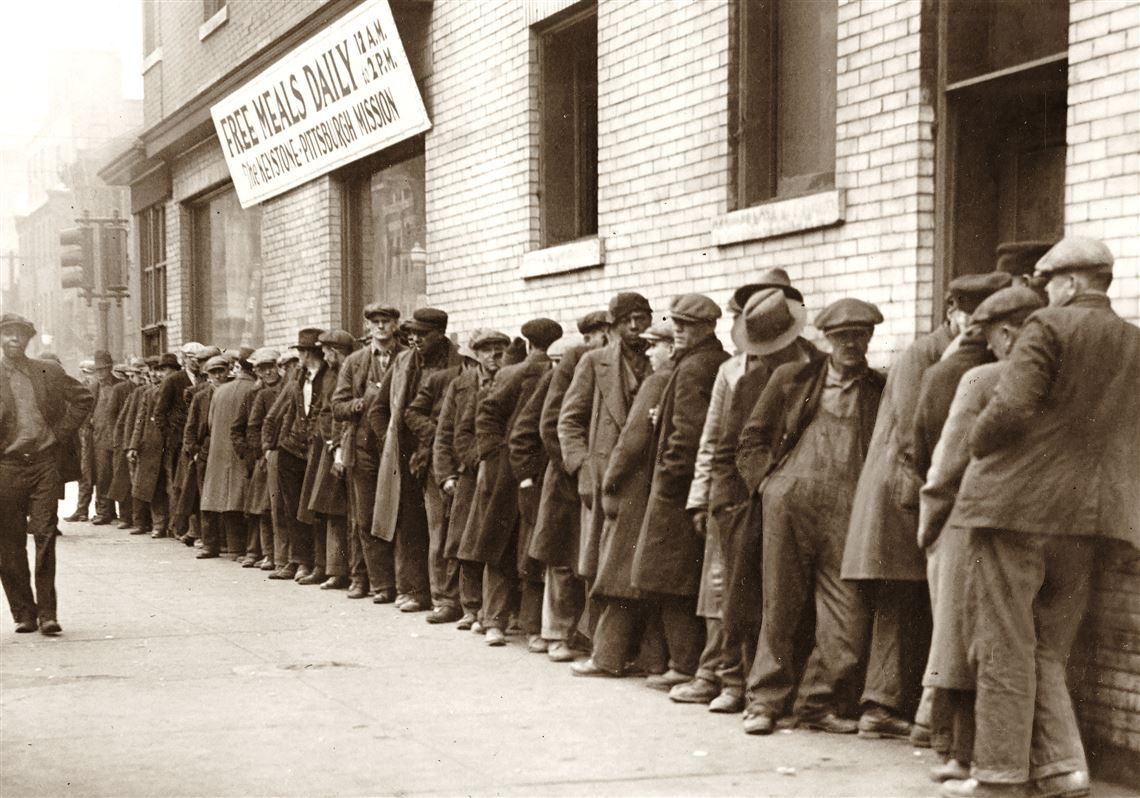
\includegraphics[width=\linewidth,height=3.125in,keepaspectratio]{files/250122/unemployment_line.jpg}

}

\caption{\label{fig-unemployment_line}Dole Queue Great Depression
(Quelle:
https://view.genially.com/609aac10d34c960d5992809a/interactive-content-great-depression-breakout,
besucht am 22.01.15).}

\end{figure}%

Für die Übungen finden Sie hier eine \href{src/nodes.py}{Klasse Node}
und eine \href{src/linked_list.py}{Klasse Linked List} zum Download.

\chapter{Queues in Python}\label{queues-in-python}

Queues sind Datenstrukturen, welche Daten speichern und grundsätzlich in
der Reihenfolge, in der sie abgespeichert worden sind, wieder
zurückgeben (First In - First Out, FIFO).\\
Eine Queue funktioniert damit wie eine Warteschlange an einer Kasse:
Wenn eine neue Person ankommt, stellt sie sich hinten an. Wenn sie die
Kasse erreicht (nachdem alle, die vorher angestanden sind, bedient
worden sind), verlässt sie die Schlange wieder.

Eine Queue ist eine derart fundamentale Datenstruktur, dass Python sie
als \href{https://docs.python.org/3/library/queue.html}{Library} zur
Verfügung stellt.

Um zu verstehen, wie eine Queue funktioniert, geht es im folgenden
darum, eine eigene Klasse Queue in Python zu implementieren.

Zu Beginn ist zu überlegen, welche Eigenschaften, die Queue aufweisen
muss. Sie muss Daten abspeichern und diese in der gleichen Reihenfolge
wieder ausgeben können. Wir brauchen also eine Struktur für die Daten
und eine Struktur, welche die Reihenfolge der Speicherung festhält. Die
Struktur, welche die Reihenfolge festhält, muss ausserdem in der Lage
sein, neue Daten abzuspeichern und bereits abgespeicherte Daten wieder
zurückzugeben. Diese Anforderungen können mit Hilfe bereits
programmierter Klassen umgesetzt werden. Um die Daten abzuspeichern,
können wir Nodes verwenden und für die Struktur zum Erhalt der
Reihenfolge die Linked List.

\begin{tcolorbox}[enhanced jigsaw, arc=.35mm, bottomrule=.15mm, bottomtitle=1mm, breakable, colback=white, colbacktitle=quarto-callout-note-color!10!white, colframe=quarto-callout-note-color-frame, coltitle=black, left=2mm, leftrule=.75mm, opacityback=0, opacitybacktitle=0.6, rightrule=.15mm, title=\textcolor{quarto-callout-note-color}{\faInfo}\hspace{0.5em}{Linked List}, titlerule=0mm, toprule=.15mm, toptitle=1mm]

Die Linked List ist eine Datenstruktur, die aus einer Anzahl von Nodes
besteht. Jeder Node hat einen Bezug auf den nächsten Node in der Liste.
Damit ist es möglich, die Nodes in einer bestimmten Reihenfolge
abzuspeichern.\\
Im Node selber gibt es ein Datenfeld \texttt{key} für die Bezeichnung
des Nodes, eines \texttt{value} für die Daten, die gespeichert werden
sollen sowie ein solches für den Verweis auf den nächsten Node. Die
Datenstruktur Linked List stellt in erster Linie den Verweis auf den
zuletzt eingefügten Node zur Verfügung.

\end{tcolorbox}

In der aktuellen Implementation der Linked List gibt es nur einen
Positionsbezug auf das letzte eingefügte Element (\texttt{self.root}).
Damit die Linked List als Queue verwendet werden kann, muss auch ein
Bezug auf das erste eingefügte Element angelegt werden
(\texttt{self.head}). Für das Erste überhaupt in die Datenstruktur
eingefügte Element ist dies kein Problem. Wenn aber weitere Elemente
eingefügt oder entfernt werden, dann muss in den einzelnen Nodes nicht
nur ein Bezug auf das folgende Element
(\texttt{self.connections{[}\textquotesingle{}next\textquotesingle{}{]}})
sondern auch einer auf das Vorangehende Element
(\texttt{self.connections{[}\textquotesingle{}previous\textquotesingle{}{]}}).
Entsprechend müssen die beiden Klassen Node und Linked List angepasst
werden.

Das kann umgesetzt werden, in dem basierend auf den bereits
existierenden Klassen abgeleitete Klassen implementiert werden. Als
UML-Klassendiagramm sieht das folgendermassen aus:

\pandocbounded{
\includegraphics[keepaspectratio]{index_files/mediabag/files/250219/class_diagram.pdf}}

Für die Umsetzung der obigen Ausführungen stehen hier zwei Module
(\href{src/linked_list.py}{linked\_list.py} und
\href{src/nodes.py}{nodes.py}) zur Verfügung.

\chapter{Binary Search Tree}\label{binary-search-tree}

Ein binärer Suchbaum (Binary Search Tree, BST) ist eine Datenstruktur,
die es ermöglicht, Daten in einer hierarchischen Struktur zu speichern.
Jeder Knoten im Baum hat maximal zwei Kinder, wobei das linke Kind
kleiner und das rechte Kind grösser als der Knoten selbst ist. Dies
ermöglicht das effiziente Suchen, Einfügen und Löschen von Elementen.

Sollen beispielsweise die Zahlen 42, 23, 17, 34, 56, 78 und 12 der Reihe
nach in einen binären Suchbaum eingefügt werden, geschieht dies wie
folgt:

\begin{verbatim}
        42
       /  \
     23    56
    /  \      \
   17   34    78
  / 
12
\end{verbatim}

Um einen Knoten zu löschen, gibt es drei Fälle zu beachten: 1. Der
Knoten ist ein Blatt (keine Kinder): Der Knoten kann einfach entfernt
werden. 2. Der Knoten hat ein Kind: Das Kind ersetzt den Knoten. 3. Der
Knoten hat zwei Kinder: Der Knoten wird durch den kleinsten Knoten im
rechten Teilbaum ersetzt.

In den folgenden Abschnitten findet sich eine Mögliche Implementierung
eines binären Suchbaums in Python.

\section{Klasse BSTNode}\label{klasse-bstnode}

\begin{Shaded}
\begin{Highlighting}[numbers=left,,]
\KeywordTok{class}\NormalTok{ BSTNode:}
    \KeywordTok{def} \FunctionTok{\_\_init\_\_}\NormalTok{(}\VariableTok{self}\NormalTok{, key, value}\OperatorTok{=}\VariableTok{None}\NormalTok{):}
        \VariableTok{self}\NormalTok{.key }\OperatorTok{=}\NormalTok{ key}
        \VariableTok{self}\NormalTok{.value }\OperatorTok{=}\NormalTok{ value}
        \VariableTok{self}\NormalTok{.parent }\OperatorTok{=} \VariableTok{None}
        \VariableTok{self}\NormalTok{.left }\OperatorTok{=} \VariableTok{None}
        \VariableTok{self}\NormalTok{.right }\OperatorTok{=} \VariableTok{None}

    \KeywordTok{def} \FunctionTok{\_\_str\_\_}\NormalTok{(}\VariableTok{self}\NormalTok{):}
\NormalTok{        key }\OperatorTok{=} \BuiltInTok{str}\NormalTok{(}\VariableTok{self}\NormalTok{.key)}
\NormalTok{        parent }\OperatorTok{=} \StringTok{\textquotesingle{}None\textquotesingle{}} \ControlFlowTok{if} \VariableTok{self}\NormalTok{.parent }\KeywordTok{is} \VariableTok{None} \ControlFlowTok{else} \BuiltInTok{str}\NormalTok{(}\VariableTok{self}\NormalTok{.parent.key)}
\NormalTok{        left }\OperatorTok{=} \StringTok{\textquotesingle{}None\textquotesingle{}} \ControlFlowTok{if} \VariableTok{self}\NormalTok{.left }\KeywordTok{is} \VariableTok{None} \ControlFlowTok{else} \BuiltInTok{str}\NormalTok{(}\VariableTok{self}\NormalTok{.left.key)}
\NormalTok{        right }\OperatorTok{=} \StringTok{\textquotesingle{}None\textquotesingle{}} \ControlFlowTok{if} \VariableTok{self}\NormalTok{.right }\KeywordTok{is} \VariableTok{None} \ControlFlowTok{else} \BuiltInTok{str}\NormalTok{(}\VariableTok{self}\NormalTok{.right.key)}
\NormalTok{        s }\OperatorTok{=}\NormalTok{ (}
            \SpecialStringTok{f\textquotesingle{}}\CharTok{\textbackslash{}t}\SpecialStringTok{Parent = }\SpecialCharTok{\{}\NormalTok{parent}\SpecialCharTok{\}}\CharTok{\textbackslash{}n}\SpecialStringTok{\textquotesingle{}}
            \SpecialStringTok{f\textquotesingle{}}\CharTok{\textbackslash{}t}\SpecialStringTok{Key = }\SpecialCharTok{\{}\NormalTok{key}\SpecialCharTok{\}}\CharTok{\textbackslash{}n}\SpecialStringTok{\textquotesingle{}}
            \SpecialStringTok{f\textquotesingle{}Left = }\SpecialCharTok{\{}\NormalTok{left}\SpecialCharTok{\}}\CharTok{\textbackslash{}t}\SpecialStringTok{Right = }\SpecialCharTok{\{}\NormalTok{right}\SpecialCharTok{\}}\SpecialStringTok{\textquotesingle{}}
\NormalTok{        )}
        \ControlFlowTok{return}\NormalTok{ s}
\end{Highlighting}
\end{Shaded}

\section{Klasse BST}\label{klasse-bst}

\begin{Shaded}
\begin{Highlighting}[numbers=left,,]
\KeywordTok{class}\NormalTok{ BST:}
    \KeywordTok{def} \FunctionTok{\_\_init\_\_}\NormalTok{(}\VariableTok{self}\NormalTok{, key}\OperatorTok{=}\VariableTok{None}\NormalTok{, value}\OperatorTok{=}\VariableTok{None}\NormalTok{):}
        \ControlFlowTok{if}\NormalTok{ key }\KeywordTok{is} \VariableTok{None}\NormalTok{:}
            \VariableTok{self}\NormalTok{.root }\OperatorTok{=} \VariableTok{None}
        \ControlFlowTok{else}\NormalTok{:}
\NormalTok{            node }\OperatorTok{=}\NormalTok{ BSTNode(key, value)            }
            \VariableTok{self}\NormalTok{.root }\OperatorTok{=}\NormalTok{ node}
            
    \KeywordTok{def}\NormalTok{ insert(}\VariableTok{self}\NormalTok{, key, value}\OperatorTok{=}\VariableTok{None}\NormalTok{, root}\OperatorTok{=}\VariableTok{None}\NormalTok{):}
\NormalTok{        node }\OperatorTok{=}\NormalTok{ BSTNode(key, value)}
        \ControlFlowTok{if} \VariableTok{self}\NormalTok{.root }\KeywordTok{is} \VariableTok{None}\NormalTok{:}
            \VariableTok{self}\NormalTok{.root }\OperatorTok{=}\NormalTok{ node}
            \ControlFlowTok{return}

        \ControlFlowTok{if}\NormalTok{ root }\KeywordTok{is} \VariableTok{None}\NormalTok{:}
\NormalTok{            root }\OperatorTok{=} \VariableTok{self}\NormalTok{.root}
        
        \ControlFlowTok{if}\NormalTok{ key }\OperatorTok{\textless{}}\NormalTok{ root.key }\KeywordTok{and}\NormalTok{ root.left }\KeywordTok{is} \VariableTok{None}\NormalTok{:}
\NormalTok{            root.left }\OperatorTok{=}\NormalTok{ node}
\NormalTok{            node.parent }\OperatorTok{=}\NormalTok{ root}
            \ControlFlowTok{return}

        \ControlFlowTok{if}\NormalTok{ key }\OperatorTok{\textless{}}\NormalTok{ root.key:}
\NormalTok{            root }\OperatorTok{=}\NormalTok{ root.left}
            \VariableTok{self}\NormalTok{.insert(key, value, root)}
            
        
        \ControlFlowTok{if}\NormalTok{ key }\OperatorTok{\textgreater{}}\NormalTok{ root.key }\KeywordTok{and}\NormalTok{ root.right }\KeywordTok{is} \VariableTok{None}\NormalTok{:}
\NormalTok{            root.right }\OperatorTok{=}\NormalTok{ node}
\NormalTok{            node.parent }\OperatorTok{=}\NormalTok{ root}
            \ControlFlowTok{return}

        \ControlFlowTok{if}\NormalTok{ key }\OperatorTok{\textgreater{}}\NormalTok{ root.key:}
\NormalTok{            root }\OperatorTok{=}\NormalTok{ root.right}
            \VariableTok{self}\NormalTok{.insert(key, value, root)}

    \KeywordTok{def} \BuiltInTok{min}\NormalTok{(}\VariableTok{self}\NormalTok{, bst}\OperatorTok{=}\VariableTok{None}\NormalTok{):}
        \ControlFlowTok{if}\NormalTok{ bst }\KeywordTok{is} \VariableTok{None}\NormalTok{:}
\NormalTok{            minimum }\OperatorTok{=} \VariableTok{self}\NormalTok{.root}
        \ControlFlowTok{else}\NormalTok{:}
\NormalTok{            minimum }\OperatorTok{=}\NormalTok{bst.root}
        
        \ControlFlowTok{while}\NormalTok{ minimum.left }\KeywordTok{is} \KeywordTok{not} \VariableTok{None}\NormalTok{:}
\NormalTok{            minimum }\OperatorTok{=}\NormalTok{ minimum.left}
        
        \ControlFlowTok{return}\NormalTok{ minimum}

    \KeywordTok{def} \BuiltInTok{max}\NormalTok{(}\VariableTok{self}\NormalTok{, bst}\OperatorTok{=}\VariableTok{None}\NormalTok{):}
        \ControlFlowTok{if}\NormalTok{ bst }\KeywordTok{is} \VariableTok{None}\NormalTok{:}
\NormalTok{            maximum }\OperatorTok{=} \VariableTok{self}\NormalTok{.root}
        \ControlFlowTok{else}\NormalTok{:}
\NormalTok{            maximum }\OperatorTok{=}\NormalTok{ bst.root}

        \ControlFlowTok{while}\NormalTok{ maximum.right }\KeywordTok{is} \KeywordTok{not} \VariableTok{None}\NormalTok{:}
\NormalTok{            maximum }\OperatorTok{=}\NormalTok{ maximum.right}

        \ControlFlowTok{return}\NormalTok{ maximum}

    \KeywordTok{def}\NormalTok{ search(}\VariableTok{self}\NormalTok{, key, node}\OperatorTok{=}\VariableTok{None}\NormalTok{):}
        \CommentTok{\# If initial call or we\textquotesingle{}ve hit None in recursion}
        \ControlFlowTok{if}\NormalTok{ node }\KeywordTok{is} \VariableTok{None}\NormalTok{:}
            \ControlFlowTok{if} \VariableTok{self}\NormalTok{.root }\KeywordTok{is} \VariableTok{None}\NormalTok{:  }\CommentTok{\# Empty tree}
                \ControlFlowTok{return} \OperatorTok{{-}}\DecValTok{1}
\NormalTok{            node }\OperatorTok{=} \VariableTok{self}\NormalTok{.root}
        
        \CommentTok{\# Found the key}
        \ControlFlowTok{if}\NormalTok{ key }\OperatorTok{==}\NormalTok{ node.key:}
            \ControlFlowTok{return}\NormalTok{ node}
            
        \CommentTok{\# Key doesn\textquotesingle{}t exist in this path}
        \ControlFlowTok{if}\NormalTok{ key }\OperatorTok{\textless{}}\NormalTok{ node.key:}
            \ControlFlowTok{if}\NormalTok{ node.left }\KeywordTok{is} \VariableTok{None}\NormalTok{:}
                \ControlFlowTok{return} \OperatorTok{{-}}\DecValTok{1}
            \ControlFlowTok{return} \VariableTok{self}\NormalTok{.search(key, node.left)}
        \ControlFlowTok{else}\NormalTok{:  }\CommentTok{\# key \textgreater{} node.key}
            \ControlFlowTok{if}\NormalTok{ node.right }\KeywordTok{is} \VariableTok{None}\NormalTok{:}
                \ControlFlowTok{return} \OperatorTok{{-}}\DecValTok{1}
            \ControlFlowTok{return} \VariableTok{self}\NormalTok{.search(key, node.right)}

    \KeywordTok{def}\NormalTok{ delete(}\VariableTok{self}\NormalTok{, key):}
        \CommentTok{\# Find the node to delete}
\NormalTok{        node }\OperatorTok{=} \VariableTok{self}\NormalTok{.search(key)}
        
        \CommentTok{\# If node not found, return}
        \ControlFlowTok{if}\NormalTok{ node }\OperatorTok{==} \OperatorTok{{-}}\DecValTok{1}\NormalTok{:}
            \ControlFlowTok{return}
        
        \VariableTok{self}\NormalTok{.\_delete\_node(node)}
        
    \KeywordTok{def}\NormalTok{ \_delete\_node(}\VariableTok{self}\NormalTok{, node):}
        \CommentTok{\# Case 1: Node has no children (leaf node)}
        \ControlFlowTok{if}\NormalTok{ node.left }\KeywordTok{is} \VariableTok{None} \KeywordTok{and}\NormalTok{ node.right }\KeywordTok{is} \VariableTok{None}\NormalTok{:}
            \ControlFlowTok{if}\NormalTok{ node }\OperatorTok{==} \VariableTok{self}\NormalTok{.root:}
                \VariableTok{self}\NormalTok{.root }\OperatorTok{=} \VariableTok{None}
            \ControlFlowTok{else}\NormalTok{:}
                \ControlFlowTok{if}\NormalTok{ node.parent.left }\OperatorTok{==}\NormalTok{ node:}
\NormalTok{                    node.parent.left }\OperatorTok{=} \VariableTok{None}
                \ControlFlowTok{else}\NormalTok{:}
\NormalTok{                    node.parent.right }\OperatorTok{=} \VariableTok{None}
        
        \CommentTok{\# Case 2: Node has only one child}
        \ControlFlowTok{elif}\NormalTok{ node.left }\KeywordTok{is} \VariableTok{None}\NormalTok{:  }\CommentTok{\# Has only right child}
            \ControlFlowTok{if}\NormalTok{ node }\OperatorTok{==} \VariableTok{self}\NormalTok{.root:}
                \VariableTok{self}\NormalTok{.root }\OperatorTok{=}\NormalTok{ node.right}
\NormalTok{                node.right.parent }\OperatorTok{=} \VariableTok{None}
            \ControlFlowTok{else}\NormalTok{:}
                \ControlFlowTok{if}\NormalTok{ node.parent.left }\OperatorTok{==}\NormalTok{ node:}
\NormalTok{                    node.parent.left }\OperatorTok{=}\NormalTok{ node.right}
                \ControlFlowTok{else}\NormalTok{:}
\NormalTok{                    node.parent.right }\OperatorTok{=}\NormalTok{ node.right}
\NormalTok{                node.right.parent }\OperatorTok{=}\NormalTok{ node.parent}
        
        \ControlFlowTok{elif}\NormalTok{ node.right }\KeywordTok{is} \VariableTok{None}\NormalTok{:  }\CommentTok{\# Has only left child}
            \ControlFlowTok{if}\NormalTok{ node }\OperatorTok{==} \VariableTok{self}\NormalTok{.root:}
                \VariableTok{self}\NormalTok{.root }\OperatorTok{=}\NormalTok{ node.left}
\NormalTok{                node.left.parent }\OperatorTok{=} \VariableTok{None}
            \ControlFlowTok{else}\NormalTok{:}
                \ControlFlowTok{if}\NormalTok{ node.parent.left }\OperatorTok{==}\NormalTok{ node:}
\NormalTok{                    node.parent.left }\OperatorTok{=}\NormalTok{ node.left}
                \ControlFlowTok{else}\NormalTok{:}
\NormalTok{                    node.parent.right }\OperatorTok{=}\NormalTok{ node.left}
\NormalTok{                node.left.parent }\OperatorTok{=}\NormalTok{ node.parent}
        
        \CommentTok{\# Case 3: Node has two children}
        \ControlFlowTok{else}\NormalTok{:}
            \CommentTok{\# Find successor (smallest node in right subtree)}
\NormalTok{            successor }\OperatorTok{=} \VariableTok{None}
\NormalTok{            current }\OperatorTok{=}\NormalTok{ node.right}
            
            \ControlFlowTok{while}\NormalTok{ current.left }\KeywordTok{is} \KeywordTok{not} \VariableTok{None}\NormalTok{:}
\NormalTok{                current }\OperatorTok{=}\NormalTok{ current.left}
            
\NormalTok{            successor }\OperatorTok{=}\NormalTok{ current}
            
            \CommentTok{\# Copy successor\textquotesingle{}s key and value to the node}
\NormalTok{            node.key }\OperatorTok{=}\NormalTok{ successor.key}
\NormalTok{            node.value }\OperatorTok{=}\NormalTok{ successor.value}
            
            \CommentTok{\# Delete the successor (which has at most one right child)}
            \VariableTok{self}\NormalTok{.\_delete\_node(successor)}
        
    \KeywordTok{def}\NormalTok{ iterate(}\VariableTok{self}\NormalTok{, node}\OperatorTok{=}\VariableTok{None}\NormalTok{, result}\OperatorTok{=}\VariableTok{None}\NormalTok{):}
        \CommentTok{\# Initialize result list on first call}
        \ControlFlowTok{if}\NormalTok{ result }\KeywordTok{is} \VariableTok{None}\NormalTok{:}
\NormalTok{            result }\OperatorTok{=}\NormalTok{ []}
        
        \CommentTok{\# Use root if no starting node provided}
        \ControlFlowTok{if}\NormalTok{ node }\KeywordTok{is} \VariableTok{None}\NormalTok{:}
            \ControlFlowTok{if} \VariableTok{self}\NormalTok{.root }\KeywordTok{is} \VariableTok{None}\NormalTok{:  }\CommentTok{\# Empty tree}
                \ControlFlowTok{return}\NormalTok{ result}
\NormalTok{            node }\OperatorTok{=} \VariableTok{self}\NormalTok{.root}
        
        \CommentTok{\# In{-}order traversal: left {-}\textgreater{} current {-}\textgreater{} right}
        \ControlFlowTok{if}\NormalTok{ node.left }\KeywordTok{is} \KeywordTok{not} \VariableTok{None}\NormalTok{:}
            \VariableTok{self}\NormalTok{.iterate(node.left, result)}
        
\NormalTok{        result.append(node)}
        
        \ControlFlowTok{if}\NormalTok{ node.right }\KeywordTok{is} \KeywordTok{not} \VariableTok{None}\NormalTok{:}
            \VariableTok{self}\NormalTok{.iterate(node.right, result)}
        
        \ControlFlowTok{return}\NormalTok{ result}
\end{Highlighting}
\end{Shaded}

\chapter{Das Binärsystem}\label{das-binuxe4rsystem}

Wir sind es gewohnt uns im Dezimalsystem zu bewegen. Das bedeutet, dass
wir Zahlen in der Basis 10 darstellen. Wir verwenden dazu 10
verschiedene Ziffern, nämlich die Ziffern 0 bis 9.\\
Um Zahlen darzustellen, welche grösser sind als 9 darzustellen,
verwenden wir die Zehnerpotenzen. Das heisst, dass die Ziffern von
rechts nach links gelesen, die Zehnerpotenzen von 0 an aufsteigend sind.
Die Zahl 123 entspricht also der Rechnung
\(1 \cdot 10^2 + 2 \cdot 10^1 + 3 \cdot 10^0\).

Das Binärsystem funktioniert nach dem gleichen Prinzip, nur dass wir nur
die Ziffern 0 und 1 verwenden. Das bedeutet, dass wir Zahlen in der
Basis 2 darstellen. Sobald eine Zahl grösser als 1 dargestellt werden
soll, schreiben wir die Zahl als Summe von Zweierpotenzen. Die Zahl 101
entspricht also der Rechnung
\(1 \cdot 2^2 + 0 \cdot 2^1 + 1 \cdot 2^0\).

\section{Umrechnung von Dezimalzahlen in
Binärzahlen}\label{umrechnung-von-dezimalzahlen-in-binuxe4rzahlen}

Um eine Dezimalzahl in eine Binärzahl umzurechnen, gibt es eine
systematische Methode, die auf wiederholter Division durch 2 basiert:

\begin{enumerate}
\def\labelenumi{\arabic{enumi}.}
\tightlist
\item
  Teile die Dezimalzahl durch 2 und notiere den Rest (0 oder 1).
\item
  Teile den Quotienten (Ergebnis der Division) erneut durch 2 und
  notiere wieder den Rest.
\item
  Fahre damit fort, bis der Quotient 0 ist.
\item
  Die Binärzahl wird nun gebildet, indem man die Reste von unten nach
  oben (vom letzten zum ersten) liest.
\end{enumerate}

\subsection{Beispiel: Umrechnung von 42 ins
Binärsystem}\label{beispiel-umrechnung-von-42-ins-binuxe4rsystem}

Lassen Sie uns die Dezimalzahl 42 in eine Binärzahl umrechnen:

{\def\LTcaptype{none} % do not increment counter
\begin{longtable}[]{@{}llll@{}}
\toprule\noalign{}
Division & Rechnung & Quotient & Rest \\
\midrule\noalign{}
\endhead
\bottomrule\noalign{}
\endlastfoot
42 ÷ 2 & 42 = 21 · 2 + 0 & 21 & 0 \\
21 ÷ 2 & 21 = 10 · 2 + 1 & 10 & 1 \\
10 ÷ 2 & 10 = 5 · 2 + 0 & 5 & 0 \\
5 ÷ 2 & 5 = 2 · 2 + 1 & 2 & 1 \\
2 ÷ 2 & 2 = 1 · 2 + 0 & 1 & 0 \\
1 ÷ 2 & 1 = 0 · 2 + 1 & 0 & 1 \\
\end{longtable}
}

Nun lesen wir die Reste von unten nach oben: 101010

Also ist 42 im Dezimalsystem gleich 101010 im Binärsystem.

\subsection{Überprüfung:}\label{uxfcberpruxfcfung}

\(1 \cdot 2^5 + 0 \cdot 2^4 + 1 \cdot 2^3 + 0 \cdot 2^2 + 1 \cdot 2^1 + 0 \cdot 2^0\)
\(= 32 + 0 + 8 + 0 + 2 + 0 = 42\)

Eine alternative Methode zur Umrechnung ist die Verwendung der
Zweierpotenzen. Man zerlegt die Dezimalzahl in eine Summe von
Zweierpotenzen und schreibt dann eine 1 an den Stellen der verwendeten
Potenzen und eine 0 an allen anderen Stellen.

\section{Umrechnung von Binärzahlen in
Dezimalzahlen}\label{umrechnung-von-binuxe4rzahlen-in-dezimalzahlen}

Die Umrechnung von Binärzahlen in Dezimalzahlen ist vergleichsweise
einfach und basiert auf der Berechnung der Stellenwerte im Binärsystem.

\subsection{Methode:}\label{methode}

\begin{enumerate}
\def\labelenumi{\arabic{enumi}.}
\tightlist
\item
  Identifiziere jede Stelle in der Binärzahl und ihre Position (von
  rechts nach links beginnend bei 0).
\item
  Multipliziere jede Binärziffer (0 oder 1) mit dem Wert von 2 hoch der
  Stellenposition.
\item
  Addiere alle resultierenden Werte zusammen.
\end{enumerate}

\subsection{Beispiel: Umrechnung von 10110₂ ins
Dezimalsystem}\label{beispiel-umrechnung-von-10110ux2082-ins-dezimalsystem}

Lassen Sie uns die Binärzahl 10110 in eine Dezimalzahl umrechnen:

{\def\LTcaptype{none} % do not increment counter
\begin{longtable}[]{@{}llllll@{}}
\toprule\noalign{}
Position (von rechts) & 4 & 3 & 2 & 1 & 0 \\
\midrule\noalign{}
\endhead
\bottomrule\noalign{}
\endlastfoot
Binäre Ziffer & 1 & 0 & 1 & 1 & 0 \\
Berechnung & 1 · 2⁴ & 0 · 2³ & 1 · 2² & 1 · 2¹ & 0 · 2⁰ \\
Dezimalwert & 16 & 0 & 4 & 2 & 0 \\
\end{longtable}
}

Nun addieren wir alle Dezimalwerte: 16 + 0 + 4 + 2 + 0 = 22

Also ist 10110₂ im Binärsystem gleich 22 im Dezimalsystem.

\subsection{Formel:}\label{formel}

Für eine Binärzahl mit n Stellen (b₀, b₁, \ldots, bₙ₋₁) gilt:

Dezimalzahl = b₀ · 2⁰ + b₁ · 2¹ + b₂ · 2² + \ldots{} + bₙ₋₁ · 2ⁿ⁻¹

wobei b₀ die erste Stelle von rechts ist.

\subsection{Praktischer Trick:}\label{praktischer-trick}

Bei der Umrechnung kann man auch eine Tabelle mit den Stellenwerten
erstellen:

{\def\LTcaptype{none} % do not increment counter
\begin{longtable}[]{@{}llllllll@{}}
\toprule\noalign{}
2⁷ & 2⁶ & 2⁵ & 2⁴ & 2³ & 2² & 2¹ & 2⁰ \\
\midrule\noalign{}
\endhead
\bottomrule\noalign{}
\endlastfoot
128 & 64 & 32 & 16 & 8 & 4 & 2 & 1 \\
\end{longtable}
}

Man schreibt die Binärzahl unter die Tabelle und addiert nur die Werte,
an deren Position eine 1 steht.

\section{Binärcodierung von
Strings}\label{binuxe4rcodierung-von-strings}

In der Informatik werden Textzeichen (Strings) durch binäre Codes
repräsentiert. Bei Unicode-Zeichen wird eine fortschrittliche Codierung
verwendet, um sowohl einfache als auch komplexe Schriftzeichen aus allen
Sprachen der Welt darstellen zu können.

\subsection{Unicode: Ein universeller
Zeichencode}\label{unicode-ein-universeller-zeichencode}

Unicode ist ein internationaler Standard zur Darstellung von Textzeichen
aller Schriftsysteme. Jedes Zeichen erhält eine eindeutige Nummer
(Codepoint), z.B. hat der Buchstabe ``A'' den Codepoint U+0041 (dezimal:
65).

\subsection{UTF-8: Die häufigste
Unicode-Codierung}\label{utf-8-die-huxe4ufigste-unicode-codierung}

UTF-8 ist die am weitesten verbreitete Codierungsform für Unicode. Sie
hat folgende Eigenschaften:

\begin{enumerate}
\def\labelenumi{\arabic{enumi}.}
\tightlist
\item
  \textbf{Variable Länge}: Ein Zeichen wird mit 1 bis 4 Bytes codiert
\item
  \textbf{Abwärtskompatibilität}: ASCII-Zeichen (0-127) werden mit nur 1
  Byte dargestellt
\item
  \textbf{Selbstsynchronisierend}: Der Anfang eines Zeichens ist
  eindeutig erkennbar
\end{enumerate}

\subsection{UTF-8 Codierungsschema:}\label{utf-8-codierungsschema}

{\def\LTcaptype{none} % do not increment counter
\begin{longtable}[]{@{}lll@{}}
\toprule\noalign{}
Anzahl Bytes & Binärmuster & Codepoint-Bereich \\
\midrule\noalign{}
\endhead
\bottomrule\noalign{}
\endlastfoot
1 & \texttt{0xxxxxxx} & U+0000 bis U+007F \\
2 & \texttt{110xxxxx\ 10xxxxxx} & U+0080 bis U+07FF \\
3 & \texttt{1110xxxx\ 10xxxxxx\ 10xxxxxx} & U+0800 bis U+FFFF \\
4 & \texttt{11110xxx\ 10xxxxxx\ 10xxxxxx\ 10xxxxxx} & U+10000 bis
U+10FFFF \\
\end{longtable}
}

Die mit \texttt{x} markierten Stellen werden mit den Bits des
Unicode-Codepoints gefüllt.

\subsection{Beispiel: Codierung deutscher
Umlaute}\label{beispiel-codierung-deutscher-umlaute}

Nehmen wir als Beispiel den Buchstaben ``ü'' (U+00FC):

\begin{enumerate}
\def\labelenumi{\arabic{enumi}.}
\tightlist
\item
  Der Codepoint von ``ü'' ist U+00FC (dezimal: 252)
\item
  Als Binärzahl: 11111100
\item
  Da der Wert \textgreater{} 127 ist, benötigen wir 2 Bytes
\item
  Nach dem 2-Byte-Schema: \texttt{110xxxxx\ 10xxxxxx}
\item
  Wir füllen den Unicode-Wert ein: \texttt{110(00000)\ 10(111100)} →
  \texttt{11000011\ 10111100}
\item
  Somit wird ``ü'' als die zwei Bytes \texttt{11000011\ 10111100}
  codiert
\end{enumerate}

\subsection{Weiteres Beispiel: Das Euro-Zeichen
€}\label{weiteres-beispiel-das-euro-zeichen}

\begin{enumerate}
\def\labelenumi{\arabic{enumi}.}
\tightlist
\item
  Der Codepoint von ``€'' ist U+20AC (dezimal: 8364)
\item
  Als Binärzahl: 10000010101100
\item
  Da der Wert \textgreater{} 2047 ist, benötigen wir 3 Bytes
\item
  Nach dem 3-Byte-Schema: \texttt{1110xxxx\ 10xxxxxx\ 10xxxxxx}
\item
  Wir füllen den Unicode-Wert ein:
  \texttt{1110(0010)\ 10(000010)\ 10(101100)} →
  \texttt{11100010\ 10000010\ 10101100}
\item
  Somit wird ``€'' als die drei Bytes
  \texttt{11100010\ 10000010\ 10101100} codiert
\end{enumerate}

\subsection{Beispiel: `Informatik ist
interessant.'}\label{beispiel-informatik-ist-interessant.}

Lassen Sie uns den Satz ``Informatik ist interessant.'' in die binäre
UTF-8-Kodierung umwandeln:

{\def\LTcaptype{none} % do not increment counter
\begin{longtable}[]{@{}lllll@{}}
\toprule\noalign{}
Zeichen & Unicode-Codepoint & Dezimal & Binär & UTF-8 Kodierung \\
\midrule\noalign{}
\endhead
\bottomrule\noalign{}
\endlastfoot
I & U+0049 & 73 & 1001001 & 01001001 \\
n & U+006E & 110 & 1101110 & 01101110 \\
f & U+0066 & 102 & 1100110 & 01100110 \\
o & U+006F & 111 & 1101111 & 01101111 \\
r & U+0072 & 114 & 1110010 & 01110010 \\
m & U+006D & 109 & 1101101 & 01101101 \\
a & U+0061 & 97 & 1100001 & 01100001 \\
t & U+0074 & 116 & 1110100 & 01110100 \\
i & U+0069 & 105 & 1101001 & 01101001 \\
k & U+006B & 107 & 1101011 & 01101011 \\
␣ & U+0020 & 32 & 100000 & 00100000 \\
i & U+0069 & 105 & 1101001 & 01101001 \\
s & U+0073 & 115 & 1110011 & 01110011 \\
t & U+0074 & 116 & 1110100 & 01110100 \\
␣ & U+0020 & 32 & 100000 & 00100000 \\
i & U+0069 & 105 & 1101001 & 01101001 \\
n & U+006E & 110 & 1101110 & 01101110 \\
t & U+0074 & 116 & 1110100 & 01110100 \\
e & U+0065 & 101 & 1100101 & 01100101 \\
r & U+0072 & 114 & 1110010 & 01110010 \\
e & U+0065 & 101 & 1100101 & 01100101 \\
s & U+0073 & 115 & 1110011 & 01110011 \\
s & U+0073 & 115 & 1110011 & 01110011 \\
a & U+0061 & 97 & 1100001 & 01100001 \\
n & U+006E & 110 & 1101110 & 01101110 \\
t & U+0074 & 116 & 1110100 & 01110100 \\
. & U+002E & 46 & 101110 & 00101110 \\
\end{longtable}
}

Da alle Zeichen in diesem Beispiel im ASCII-Bereich liegen (0-127), wird
jedes Zeichen mit genau einem Byte codiert. Der vollständige Text
benötigt also 27 Bytes im UTF-8 Format.

Die komplette binäre Darstellung des Textes ist:

\begin{verbatim}
01001001 01101110 01100110 01101111 01110010 01101101 01100001 01110100 
01101001 01101011 00100000 01101001 01110011 01110100 00100000 01101001 
01101110 01110100 01100101 01110010 01100101 01110011 01110011 01100001 
01101110 01110100 00101110
\end{verbatim}

In hexadezimaler Schreibweise:

\begin{verbatim}
49 6E 66 6F 72 6D 61 74 69 6B 20 69 73 74 20 69 6E 74 65 72 65 73 73 61 6E 74 2E
\end{verbatim}

Dieser String kann direkt in einem Computer gespeichert und verarbeitet
werden. In Textdateien, bei der Übertragung im Internet oder in
Datenbanken sind Strings immer in solchen binären Formaten gespeichert.

\subsection{Vorteile der
Unicode-Codierung:}\label{vorteile-der-unicode-codierung}

\begin{enumerate}
\def\labelenumi{\arabic{enumi}.}
\tightlist
\item
  \textbf{Universalität}: Alle Schriftsysteme und Sonderzeichen können
  dargestellt werden
\item
  \textbf{Effizienz}: Häufig verwendete Zeichen benötigen weniger
  Speicherplatz
\item
  \textbf{Kompatibilität}: Rückwärtskompatibel mit ASCII, was die
  Integration erleichtert
\end{enumerate}

Die Umwandlung zwischen Textzeichen und ihrer binären Repräsentation
wird in Computersystemen automatisch durch Codierungs- und
Decodierungsprozesse abgewickelt, sodass Benutzer sich in der Regel
nicht mit den Details befassen müssen.

\chapter{Python Funktionen zum Umrechnen zwichen den
Zahlensystemen}\label{python-funktionen-zum-umrechnen-zwichen-den-zahlensystemen}

Python stellt Funktionen zur Verfügung, mit deren Hilfe Zahlen zwischen
den verschiedenen Zahlensystemen umgerechnet werden können. Trotzdem
sollen in diesem Notebook eigene Funktionen implementiert werden, mit
deren Hilfe Zahlen zwischen dem Dezimal- und Binärsystem umgerechnet
werden können.

Ausserdem sollen Funktionen implementiert werden, mit welchen Strings in
ihre binäre Repräsentation umgewandelt werden können und umgekehrt.

\section{Umrechnung von Binär- in
Dezimalzahlen}\label{umrechnung-von-binuxe4r--in-dezimalzahlen}

\begin{Shaded}
\begin{Highlighting}[numbers=left,,]
\KeywordTok{def}\NormalTok{ bin2dec(binary: }\BuiltInTok{str}\NormalTok{) }\OperatorTok{{-}\textgreater{}} \BuiltInTok{int}\NormalTok{:}
    \CommentTok{\# }\AlertTok{TODO}\CommentTok{: implementieren Sie hier die Funktion}
    \ControlFlowTok{pass}
        
\end{Highlighting}
\end{Shaded}

\section{Umrechnung von Dezimal- in
Binärzahlen}\label{umrechnung-von-dezimal--in-binuxe4rzahlen}

\begin{Shaded}
\begin{Highlighting}[numbers=left,,]
\KeywordTok{def}\NormalTok{ dec2bin(decimal: }\BuiltInTok{int}\NormalTok{) }\OperatorTok{{-}\textgreater{}} \BuiltInTok{str}\NormalTok{:}
    \CommentTok{\# }\AlertTok{TODO}\CommentTok{: implementieren Sie hier die Funktion}
    \ControlFlowTok{pass}
\end{Highlighting}
\end{Shaded}

\section{Binäre Repräsentation von
Strings}\label{binuxe4re-repruxe4sentation-von-strings}

Für die Darstellung eines Strings in binärer Form wird auf die dezimale
Repräsentation des Unicode-Zeichens zurückgegriffen. Dazu stellt Python
die Funktion \texttt{ord()} zur Verfügung. Diese Funktion gibt die
dezimale Repräsentation eines Unicode-Zeichens zurück.

\begin{Shaded}
\begin{Highlighting}[numbers=left,,]
\KeywordTok{def}\NormalTok{ str2bin(s: }\BuiltInTok{str}\NormalTok{) }\OperatorTok{{-}\textgreater{}} \BuiltInTok{str}\NormalTok{:}
    \CommentTok{\# }\AlertTok{TODO}\CommentTok{: implementieren Sie hier die Funktion}
    \ControlFlowTok{pass}
\end{Highlighting}
\end{Shaded}

\section{Umwandlung der binären Repräsentation in einen
String}\label{umwandlung-der-binuxe4ren-repruxe4sentation-in-einen-string}

Um aus der dezimalen Repräsentation eines Unicode-Zeichens wieder den
entsprechenden String zu erhalten, stellt Python die Funktion
\texttt{chr()} zur Verfügung.

\begin{Shaded}
\begin{Highlighting}[numbers=left,,]
\KeywordTok{def}\NormalTok{ bin2str(binary: }\BuiltInTok{str}\NormalTok{) }\OperatorTok{{-}\textgreater{}} \BuiltInTok{str}\NormalTok{:}
    \CommentTok{\# }\AlertTok{TODO}\CommentTok{: implementieren Sie hier die Funktion}
    \ControlFlowTok{pass}
\end{Highlighting}
\end{Shaded}

\chapter{Python Funktionen zum Umrechnen zwichen den
Zahlensystemen}\label{python-funktionen-zum-umrechnen-zwichen-den-zahlensystemen-1}

Python stellt Funktionen zur Verfügung, mit deren Hilfe Zahlen zwischen
den verschiedenen Zahlensystemen umgerechnet werden können. Trotzdem
sollen in diesem Notebook eigene Funktionen implementiert werden, mit
deren Hilfe Zahlen zwischen dem Dezimal- und Binärsystem umgerechnet
werden können.

Ausserdem sollen Funktionen implementiert werden, mit welchen Strings in
ihre binäre Repräsentation umgewandelt werden können und umgekehrt.

\section{Umrechnung von Binär- in
Dezimalzahlen}\label{umrechnung-von-binuxe4r--in-dezimalzahlen-1}

\begin{Shaded}
\begin{Highlighting}[numbers=left,,]
\KeywordTok{def}\NormalTok{ bin2dec(binary: }\BuiltInTok{str}\NormalTok{) }\OperatorTok{{-}\textgreater{}} \BuiltInTok{int}\NormalTok{:}
\NormalTok{    decimal }\OperatorTok{=} \DecValTok{0}
\NormalTok{    length }\OperatorTok{=} \BuiltInTok{len}\NormalTok{(binary)}
    
    \ControlFlowTok{for}\NormalTok{ i }\KeywordTok{in} \BuiltInTok{range}\NormalTok{(}\DecValTok{1}\NormalTok{, length }\OperatorTok{+} \DecValTok{1}\NormalTok{):}
\NormalTok{        decimal }\OperatorTok{+=} \BuiltInTok{int}\NormalTok{(binary[}\OperatorTok{{-}}\NormalTok{i]) }\OperatorTok{*} \DecValTok{2} \OperatorTok{**}\NormalTok{ (i}\OperatorTok{{-}}\DecValTok{1}\NormalTok{)}
        
    \ControlFlowTok{return}\NormalTok{ decimal}
        
\end{Highlighting}
\end{Shaded}

\section{Umrechnung von Dezimal- in
Binärzahlen}\label{umrechnung-von-dezimal--in-binuxe4rzahlen-1}

\begin{Shaded}
\begin{Highlighting}[numbers=left,,]
\KeywordTok{def}\NormalTok{ dec2bin(decimal: }\BuiltInTok{int}\NormalTok{) }\OperatorTok{{-}\textgreater{}} \BuiltInTok{str}\NormalTok{:}
\NormalTok{    binary }\OperatorTok{=} \StringTok{\textquotesingle{}\textquotesingle{}}
    \ControlFlowTok{while}\NormalTok{ decimal }\OperatorTok{\textgreater{}} \DecValTok{0}\NormalTok{:}
\NormalTok{        binary }\OperatorTok{=} \BuiltInTok{str}\NormalTok{(decimal }\OperatorTok{\%} \DecValTok{2}\NormalTok{) }\OperatorTok{+}\NormalTok{ binary}
\NormalTok{        decimal }\OperatorTok{=}\NormalTok{ decimal }\OperatorTok{//} \DecValTok{2}
        
    \ControlFlowTok{return}\NormalTok{ binary}
\end{Highlighting}
\end{Shaded}

\section{Binäre Repräsentation von
Strings}\label{binuxe4re-repruxe4sentation-von-strings-1}

Für die Darstellung eines Strings in binärer Form wird auf die dezimale
Repräsentation des Unicode-Zeichens zurückgegriffen. Dazu stellt Python
die Funktion \texttt{ord()} zur Verfügung. Diese Funktion gibt die
dezimale Repräsentation eines Unicode-Zeichens zurück.

\begin{Shaded}
\begin{Highlighting}[numbers=left,,]
\KeywordTok{def}\NormalTok{ str2bin(s: }\BuiltInTok{str}\NormalTok{) }\OperatorTok{{-}\textgreater{}} \BuiltInTok{str}\NormalTok{:}
\NormalTok{    length\_string }\OperatorTok{=} \BuiltInTok{len}\NormalTok{(s)}
\NormalTok{    binary }\OperatorTok{=} \StringTok{\textquotesingle{}\textquotesingle{}}
    \ControlFlowTok{for}\NormalTok{ i }\KeywordTok{in} \BuiltInTok{range}\NormalTok{(length\_string):}
\NormalTok{        c }\OperatorTok{=}\NormalTok{ s[i]}
\NormalTok{        u10 }\OperatorTok{=} \BuiltInTok{ord}\NormalTok{(c)}
\NormalTok{        b }\OperatorTok{=}\NormalTok{ dec2bin(u10)}
\NormalTok{        length\_binary }\OperatorTok{=} \BuiltInTok{len}\NormalTok{(b)}
        \ControlFlowTok{if}\NormalTok{ i }\OperatorTok{\%} \DecValTok{5} \OperatorTok{==} \DecValTok{0} \KeywordTok{and}\NormalTok{ i }\OperatorTok{!=} \DecValTok{0}\NormalTok{:}
\NormalTok{            binary }\OperatorTok{+=} \StringTok{\textquotesingle{}}\CharTok{\textbackslash{}n}\StringTok{\textquotesingle{}}
\NormalTok{        b }\OperatorTok{=} \StringTok{\textquotesingle{}0\textquotesingle{}} \OperatorTok{*}\NormalTok{ (}\DecValTok{8} \OperatorTok{{-}}\NormalTok{ length\_binary) }\OperatorTok{+}\NormalTok{ b}
\NormalTok{        binary }\OperatorTok{+=}\NormalTok{ b }\OperatorTok{+} \StringTok{\textquotesingle{} \textquotesingle{}}
    \ControlFlowTok{return}\NormalTok{ binary.strip()}
\end{Highlighting}
\end{Shaded}

\section{Umwandlung der binären Repräsentation in einen
String}\label{umwandlung-der-binuxe4ren-repruxe4sentation-in-einen-string-1}

Um aus der dezimalen Repräsentation eines Unicode-Zeichens wieder den
entsprechenden String zu erhalten, stellt Python die Funktion
\texttt{chr()} zur Verfügung.

\begin{Shaded}
\begin{Highlighting}[numbers=left,,]
\KeywordTok{def}\NormalTok{ bin2str(binary: }\BuiltInTok{str}\NormalTok{) }\OperatorTok{{-}\textgreater{}} \BuiltInTok{str}\NormalTok{:}
\NormalTok{    binary }\OperatorTok{=}\NormalTok{ binary.replace(}\StringTok{\textquotesingle{} \textquotesingle{}}\NormalTok{, }\StringTok{\textquotesingle{}\textquotesingle{}}\NormalTok{)}
\NormalTok{    binary }\OperatorTok{=}\NormalTok{ binary.replace(}\StringTok{\textquotesingle{}}\CharTok{\textbackslash{}n}\StringTok{\textquotesingle{}}\NormalTok{, }\StringTok{\textquotesingle{}\textquotesingle{}}\NormalTok{)}
\NormalTok{    length }\OperatorTok{=} \BuiltInTok{len}\NormalTok{(binary)}
\NormalTok{    s }\OperatorTok{=} \StringTok{\textquotesingle{}\textquotesingle{}}
    \ControlFlowTok{for}\NormalTok{ i }\KeywordTok{in} \BuiltInTok{range}\NormalTok{(}\DecValTok{0}\NormalTok{, length, }\DecValTok{8}\NormalTok{):}
\NormalTok{        b }\OperatorTok{=}\NormalTok{ binary[i:i}\OperatorTok{+}\DecValTok{8}\NormalTok{]}
\NormalTok{        u10 }\OperatorTok{=}\NormalTok{ bin2dec(b)}
\NormalTok{        c }\OperatorTok{=} \BuiltInTok{chr}\NormalTok{(u10)}
\NormalTok{        s }\OperatorTok{+=}\NormalTok{ c}
    \ControlFlowTok{return}\NormalTok{ s}
\end{Highlighting}
\end{Shaded}

\chapter{Base64-Codierung}\label{base64-codierung}

Die Base64-Codierung ist ein Verfahren zur Umwandlung von Binärdaten in
eine Zeichenkette, die nur aus lesbaren ASCII-Zeichen besteht. Diese
Codierung wird häufig verwendet, um binäre Daten über textbasierte
Systeme zu übertragen, die möglicherweise nicht mit Binärdaten umgehen
können (z.B. E-Mails). Eine weitere Anwendung ist die Einbettung von
Bildern in HTML- oder Markdown-Dokumente.\\
Untenstehende Octocat-Grafik ist ein Beispiel für eine Base64-codierte
Grafik.

\begin{figure}[H]

{\centering \pandocbounded{
\includegraphics[keepaspectratio]{index_files/mediabag/KKsN5DtWRIAAAAASUVOR.png}}

}

\caption{Base64 codierte Octocat}

\end{figure}%

Sofern die Website in Chrome geöffnet ist, kann die Grafik mit einem
Rechtsklick ``untersucht'' werden. Die ``Untersuchung'' zeigt den
Quellcode der Seite an. Dort kann die Base64-codierte Grafik gefunden
werden. Diese beginnt mit \texttt{data:image/png;base64,} und setzt sich
mit einer langen Zeichenkette fort. Diese Zeichenkette ist die
Base64-Codierung der Grafik.

\section{Prinzip der
Base64-Codierung}\label{prinzip-der-base64-codierung}

Base64 wandelt 3 Bytes (24 Bits) Binärdaten in 4 druckbare ASCII-Zeichen
um:

\begin{enumerate}
\def\labelenumi{\arabic{enumi}.}
\tightlist
\item
  Die Binärdaten werden in 6-Bit-Blöcke aufgeteilt (2\^{}6 = 64 mögliche
  Werte)
\item
  Jeder 6-Bit-Block wird in ein druckbares ASCII-Zeichen umgewandelt
\item
  Bei unvollständigen Blocks am Ende werden Füllzeichen (\texttt{=})
  hinzugefügt
\end{enumerate}

\section{Base64-Zeichensatz}\label{base64-zeichensatz}

Der Base64-Zeichensatz besteht aus 64 Zeichen: - Die Großbuchstaben A-Z
(26 Zeichen) - Die Kleinbuchstaben a-z (26 Zeichen) - Die Ziffern 0-9
(10 Zeichen) - Zwei zusätzliche Zeichen, meist `+' und `/' (2 Zeichen)

Diese 64 Zeichen repräsentieren die Werte 0-63 und können mit 6 Bits
dargestellt werden.

\section{Codierungsprozess}\label{codierungsprozess}

\begin{enumerate}
\def\labelenumi{\arabic{enumi}.}
\tightlist
\item
  Die Binärdaten werden in Gruppen von 3 Bytes (24 Bits) aufgeteilt
\item
  Diese 24 Bits werden in vier 6-Bit-Blöcke umgewandelt
\item
  Jeder 6-Bit-Wert wird als Index für den Base64-Zeichensatz verwendet
\end{enumerate}

Wenn die Anzahl der zu codierenden Bytes nicht durch 3 teilbar ist: -
Bei einem übrig bleibenden Byte: Auffüllen mit vier Nullbits, Codierung
ergibt zwei Zeichen und zwei `='-Zeichen - Bei zwei übrig bleibenden
Bytes: Auffüllen mit zwei Nullbits, Codierung ergibt drei Zeichen und
ein `='-Zeichen

\section{Beispiele:}\label{beispiele}

\subsection{Beispiel 1: Codierung von
``KBW''}\label{beispiel-1-codierung-von-kbw}

\begin{figure}[H]

{\centering \pandocbounded{
\includegraphics[keepaspectratio]{index_files/mediabag/files/250319/tabelle.pdf}}

}

\caption{Base64 Beispiel}

\end{figure}%

\subsection{Beispiel 2: Codierung von
``Hallo''}\label{beispiel-2-codierung-von-hallo}

Betrachten wir das Wort ``Hallo'':

\begin{enumerate}
\def\labelenumi{\arabic{enumi}.}
\tightlist
\item
  ASCII-Werte: H=72, a=97, l=108, l=108, o=111
\item
  Binär: 01001000 01100001 01101100 01101100 01101111
\item
  In 6-Bit-Gruppen aufteilen: 010010 000110 000101 101100 011011 000110
  1111
\item
  Da die letzte Gruppe nur 4 Bits hat, wird sie mit zwei Nullen
  aufgefüllt: 010010 000110 000101 101100 011011 000110 111100
\item
  Die 6-Bit-Werte sind: 18, 6, 5, 44, 27, 6, 60
\item
  Diese werden in Base64-Zeichen umgewandelt: S G F s b G 8 =
\end{enumerate}

Das Ergebnis ``SGFsbG8='' ist die Base64-Codierung von ``Hallo''.

\section{Anwendungen der
Base64-Codierung}\label{anwendungen-der-base64-codierung}

\begin{itemize}
\tightlist
\item
  E-Mail-Anhänge (MIME)
\item
  Datenkodierung in URLs
\item
  Einbettung von Bildern in HTML/CSS (Data-URLs)
\item
  Übertragung binärer Daten in JSON
\item
  Speicherung von Binärdaten in XML
\end{itemize}

Base64 vergrößert die Datenmenge um etwa 33\% (da 3 Bytes in 4 Zeichen
umgewandelt werden), bietet aber den Vorteil, dass die codierten Daten
in jedem Textformat sicher übertragen werden können.

\chapter{Lernziele für die Prüfung vom 26. März
2025}\label{lernziele-fuxfcr-die-pruxfcfung-vom-26.-muxe4rz-2025}

Ich erwarte, dass Sie in der Lage sind,

\begin{itemize}
\tightlist
\item
  die folgenden Datenstrukturen zu beschreiben und ihre Implementation
  in Python grundsätzlich zu erklären:

  \begin{itemize}
  \tightlist
  \item
    Linked List
  \item
    Stack
  \item
    Queue sowie
  \item
    Binary Search Tree;
  \end{itemize}
\item
  Zahlen vom Dezimalsystem ins Binärsystem umzurechnen und umgekehrt
  sowie
\item
  zu erklären, wozu die Base64-Codierung verwendet wird und wie sie
  funktioniert.
\end{itemize}

And der Prüfung dürfen Sie eine handschriftliche Zusammenfassung im
Umfang von einer Seite A4 verwenden. Das einzige, was nicht auf der
Zusammenfassung stehen darf, sind die für das Arbeiten mit Jupyter
Notebooks notwendigen Einrichtungsschritte.

\part{Künstliche Intelligenz}

\chapter{The Social Dilemma}\label{the-social-dilemma}

The Social Dilemma ist ein Film von Nextflix.

\url{https://www.netflix.com/title/81254224}

\chapter{Was ist eine Künstliche
Intelligenz?}\label{was-ist-eine-kuxfcnstliche-intelligenz}

Sie alle kennen heute \textbf{generative K.I.}-Tools. Wir werden zuerst
K.I. anschauen, die keinen Inhalt generieren, sondern Entscheidungen
fällen. Dies ist zu Beginn einfacher nachzuvollziehen, was ein Modell
ist.

Nehmen Sie Kopfhörer nach vorne und absolvieren Sie selbstständig diesen
Kurs:
\url{https://studio.code.org/courses/oceans/units/1/lessons/1/levels/1}

\chapter{Maschinelles Lernen: Punkt- und
Linienklassifikatoren}\label{maschinelles-lernen-punkt--und-linienklassifikatoren}

Besuchen Sie die Seite
\url{https://ricardoheinzmann.com/ml-class/level-selection}.

Spielen Sie in folgender Reihenfolge:

\begin{enumerate}
\def\labelenumi{\arabic{enumi}.}
\tightlist
\item
  \href{https://ricardoheinzmann.com/ml-class/level/linien-klassifizieren-2D}{Linien-Klassifizieren
  mit 2D-Daten}
\item
  \href{https://ricardoheinzmann.com/ml-class/level/punkt-klassifizieren-2D}{Punkt-Klassifizieren
  mit 2D-Daten}
\item
  \href{https://ricardoheinzmann.com/ml-class/level/punkt-klassifizieren-3D}{Punkt-Klassifizieren
  mit 3D-Daten}
\end{enumerate}

\chapter{Maschinelles Lernen:
Gewinnstrategie}\label{maschinelles-lernen-gewinnstrategie}

Spielen Sie das Spiel und entdecken Sie den Lernalgorithmus.

Bedienung:

\begin{itemize}
\tightlist
\item
  Klicken Sie auf einen blauen Spielstein, nachher auf das gefärbte Feld
  eins weiter unten.
\end{itemize}

https://aieducation.computatrum.ch/

Nach der ``Übung 1: Lernalgorithmus in Aktion - Einfach'' dürfen Sie
selber entscheiden, ob Sie die selbe Übung mit einem \emph{Mittel}
schweren Spiel machen möchten, oder zur Übung 2 gehen.

\part{Anleitungen}

\chapter{Installation von Python}\label{installation-von-python}

Hier ist eine einfache Schritt-für-Schritt-Anleitung zur Installation
von Python:

\section{Python herunterladen und
installieren}\label{python-herunterladen-und-installieren}

\begin{enumerate}
\def\labelenumi{\arabic{enumi}.}
\item
  Öffnen Sie Ihren Webbrowser und gehen Sie zur offiziellen
  Python-Website: \url{www.python.org}
\item
  Klicken Sie auf der Startseite auf den Button ``Downloads''
\item
  Suchen Sie die neueste Python-Version für Windows (Juli 24 Python
  3.12.x)
\item
  Klicken Sie auf den Download-Button für die 64-bit-Version (falls
  nicht automatisch ausgewählt)
\item
  Nachdem der Download abgeschlossen ist, öffnen Sie die
  heruntergeladene Datei (sie endet auf .exe)
\item
  Im Installationsfenster setzen Sie ein Häkchen bei ``Add Python x.x to
  PATH'' (\textbf{sehr wichtig!})
\item
  Klicken Sie auf ``Install Now'' und warten Sie, bis die Installation
  abgeschlossen ist
\item
  Klicken Sie am Ende auf ``Close''
\end{enumerate}

\section{Installation überprüfen}\label{installation-uxfcberpruxfcfen}

\begin{enumerate}
\def\labelenumi{\arabic{enumi}.}
\item
  Öffnen Sie die Windows-Eingabeaufforderung (\texttt{cmd}/Terminal):

  \begin{itemize}
  \tightlist
  \item
    Drücken Sie die Windows-Taste + R
  \item
    Geben Sie ``\texttt{cmd}'' ein und drücken Sie Enter
  \end{itemize}
\item
  In der Eingabeaufforderung/Terminal (dem neu aufgegangen Fenster)
  tippen Sie:

\begin{Shaded}
\begin{Highlighting}[numbers=left,,]
\ExtensionTok{python} \AttributeTok{{-}{-}version}
\end{Highlighting}
\end{Shaded}

  und drücken Sie Enter
\item
  Wenn die Installation erfolgreich war, sehen Sie die installierte
  Python-Version (stimmt mit dem Überein, was auf dem Download-Button
  gestanden hat)
\end{enumerate}

\section{Erste Schritte mit Python}\label{erste-schritte-mit-python}

\begin{enumerate}
\def\labelenumi{\arabic{enumi}.}
\item
  In der Eingabeaufforderung tippen Sie \texttt{python} und drücken
  Enter
\item
  Sie sehen nun den Python-Prompt
  (\textgreater\textgreater\textgreater). Der Prompt ist eine
  Eingabeaufforderung. Hier können Sie direkt Python-Code eingeben,
  z.B.:

\begin{Shaded}
\begin{Highlighting}[numbers=left,,]
\BuiltInTok{print}\NormalTok{(}\StringTok{"Hallo, Welt!"}\NormalTok{)}
\end{Highlighting}
\end{Shaded}
\item
  Drücken Sie Enter, um den Code auszuführen
\item
  Um die Python-Umgebung zu verlassen, geben Sie \texttt{exit()} ein und
  drücken Enter
\end{enumerate}

Glückwunsch! Sie haben Python erfolgreich installiert und Ihr erstes
Programm ausgeführt.

Mit dieser Anleitung sollten Sie Python problemlos installieren und
erste Schritte in der Programmierung machen können. Viel Erfolg beim
Lernen!

\emph{Dieser Text wurde mit Hilfe von Perplexity.ai erstellt.}

\chapter{Anleitung zum Arbeiten mit Python Virtual
Environments}\label{anleitung-zum-arbeiten-mit-python-virtual-environments}

Eine Python Virtual Environment (venv) ist eine geschützte Umgebung, in
der die Installation zusätzlicher Module zu keinen Konflikten mit dem
Gesamtsystem führen. Aus diesem Grund ist es sinnvoll, für jedes neue
Python Projekt eine solche venv anzulegen.

Hier eine Checkliste für das Arbeiten in einer venv:

Als Vorfrage ist zu prüfen, ob bereits eine venv angelegt ist.

\section{Arbeiten mit einer bereits bestehenden
venv}\label{arbeiten-mit-einer-bereits-bestehenden-venv}

\begin{enumerate}
\def\labelenumi{\arabic{enumi}.}
\item
  Aktivieren der venv:

\begin{Shaded}
\begin{Highlighting}[numbers=left,,]
\NormalTok{C:\textbackslash{}Pfad\textbackslash{}zum\textbackslash{}aktuellen\textbackslash{}Ordner\textgreater{}venv\textbackslash{}Scripts\textbackslash{}activate}
\end{Highlighting}
\end{Shaded}

  Dass die venv aktiviert worden ist, erkennt man daran, dass das
  Terminal folgenden Prompt aufweist:

\begin{Shaded}
\begin{Highlighting}[numbers=left,,]
\NormalTok{(venv) C:\textbackslash{}Pfad\textbackslash{}zum\textbackslash{}aktuellen\textbackslash{}Ordner\textgreater{}}
\end{Highlighting}
\end{Shaded}
\item
  Jupyter Server starten:

\begin{Shaded}
\begin{Highlighting}[numbers=left,,]
\NormalTok{(venv) C:\textbackslash{}Pfad\textbackslash{}zum\textbackslash{}aktuellen\textbackslash{}Ordner\textgreater{}jupyter notebook}
\end{Highlighting}
\end{Shaded}

  Das Terminal, in welchem der Jupyter Server gestartet wurde, darf
  \textbf{nicht} geschlossen werden.
\item
  Arbeiten am Projekt
\item
  Jupyter Server deaktivieren.

  Der Jupyter Server kann im Terminal, in welchem er gestartet wurde,
  mit der Tastenkombination {[}Ctrl{]} + {[}C{]} angehalten werden.
\item
  venv deaktivieren

\begin{Shaded}
\begin{Highlighting}[numbers=left,,]
\NormalTok{(venv) C:\textbackslash{}Pfad\textbackslash{}zum\textbackslash{}aktuellen\textbackslash{}Ordner\textgreater{}deactivate}
\end{Highlighting}
\end{Shaded}
\end{enumerate}

\section{Einrichten einer neuen venv}\label{einrichten-einer-neuen-venv}

\begin{enumerate}
\def\labelenumi{\arabic{enumi}.}
\item
  Projektordner erstellen
\item
  venv anlegen:

\begin{Shaded}
\begin{Highlighting}[numbers=left,,]
\NormalTok{C:\textbackslash{}Pfad\textbackslash{}zum\textbackslash{}aktuellen\textbackslash{}Ordner\textgreater{}python {-}m venv venv}
\end{Highlighting}
\end{Shaded}
\item
  Aktivieren der venv:

\begin{Shaded}
\begin{Highlighting}[numbers=left,,]
\NormalTok{C:\textbackslash{}Pfad\textbackslash{}zum\textbackslash{}aktuellen\textbackslash{}Ordner\textgreater{}venv\textbackslash{}Scripts\textbackslash{}activate}
\end{Highlighting}
\end{Shaded}

  Dass die venv aktiviert worden ist, erkennt man daran, dass das
  Terminal folgenden Prompt aufweist:

\begin{Shaded}
\begin{Highlighting}[numbers=left,,]
\NormalTok{(venv) C:\textbackslash{}Pfad\textbackslash{}zum\textbackslash{}aktuellen\textbackslash{}Ordner\textgreater{}}
\end{Highlighting}
\end{Shaded}
\item
  Installieren der erforderlichen Pakete:

\begin{Shaded}
\begin{Highlighting}[numbers=left,,]
\NormalTok{(venv) C:\textbackslash{}Pfad\textbackslash{}zum\textbackslash{}aktuellen\textbackslash{}Ordner\textgreater{}python {-}m pip install jupyter (und allfällige andere Pakete)}
\end{Highlighting}
\end{Shaded}
\item
  Jupyter Server starten:

\begin{Shaded}
\begin{Highlighting}[numbers=left,,]
\NormalTok{(venv) C:\textbackslash{}Pfad\textbackslash{}zum\textbackslash{}aktuellen\textbackslash{}Ordner\textgreater{}jupyter notebook}
\end{Highlighting}
\end{Shaded}

  Das Terminal, in welchem der Jupyter Server gestartet wurde, darf
  \textbf{nicht} geschlossen werden.
\item
  Arbeiten am Projekt
\item
  Jupyter Server deaktivieren.

  Der Jupyter Server kann im Terminal, in welchem er gestartet wurde,
  mit der Tastenkombination {[}Ctrl{]} + {[}C{]} angehalten werden.
\item
  venv deaktivieren

\begin{Shaded}
\begin{Highlighting}[numbers=left,,]
\NormalTok{(venv) C:\textbackslash{}Pfad\textbackslash{}zum\textbackslash{}aktuellen\textbackslash{}Ordner\textgreater{}deactivate}
\end{Highlighting}
\end{Shaded}
\end{enumerate}

\chapter{Jupyter Notebook}\label{jupyter-notebook}

In einem Jupyter Notebook kann Text mit ausführbarem Programmcode
kombiniert werden. Wir werden Jupyter Notebooks für die
Anwendungsübungen im Unterricht verwenden.

\section{Installationsanleitung}\label{installationsanleitung}

Hier ist eine Schritt-für-Schritt-Anleitung zur Installation von Jupyter
Notebooks:

\begin{enumerate}
\def\labelenumi{\arabic{enumi}.}
\item
  Öffnen Sie die Windows-Eingabeaufforderung (cmd).
\item
  Wechseln Sie mit

\begin{Shaded}
\begin{Highlighting}[numbers=left,,]
\BuiltInTok{cd} \DataTypeTok{\textbackslash{}P}\NormalTok{fad}\DataTypeTok{\textbackslash{}z}\NormalTok{um}\DataTypeTok{\textbackslash{}A}\NormalTok{rbeitsverzeichnis}
\end{Highlighting}
\end{Shaded}

  in Ihr Arbeitsverzeichnis.
\item
  Starten Sie eine Python Virtual Environment

\begin{Shaded}
\begin{Highlighting}[numbers=left,,]
\ExtensionTok{python} \AttributeTok{{-}m}\NormalTok{ venv venv}

\ExtensionTok{venv\textbackslash{}Scripts\textbackslash{}activate}
\end{Highlighting}
\end{Shaded}
\item
  Geben Sie folgenden Befehl ein und drücken Sie Enter:

\begin{Shaded}
\begin{Highlighting}[numbers=left,,]
\ExtensionTok{python} \AttributeTok{{-}m}\NormalTok{ pip install jupyter}
\end{Highlighting}
\end{Shaded}

  Die Installation braucht etwas Zeit. Haben Sie Geduld mit Ihrem
  Computer.

  Falls pip aus irgendeinem Grund nicht installiert wurde oder nicht
  funktioniert, können Sie es manuell installieren, indem Sie den
  folgenden Befehl in der Eingabeaufforderung ausführen:

\begin{Shaded}
\begin{Highlighting}[numbers=left,,]
\ExtensionTok{python} \AttributeTok{{-}m}\NormalTok{ ensurepip }\AttributeTok{{-}{-}upgrade}
\end{Highlighting}
\end{Shaded}

  Dieser Befehl stellt sicher, dass pip installiert und auf dem neuesten
  Stand ist.
\end{enumerate}

\section{Jupyter Notebook starten}\label{jupyter-notebook-starten}

\begin{enumerate}
\def\labelenumi{\arabic{enumi}.}
\item
  Öffnen Sie erneut die Eingabeaufforderung/das Terminal.
\item
  Geben Sie ein:

\begin{verbatim}
jupyter notebook
\end{verbatim}
\item
  Drücken Sie Enter. Ihr Standardbrowser öffnet sich automatisch mit der
  Jupyter Notebook-Oberfläche.
\end{enumerate}

\section{Ihr erstes Notebook
erstellen}\label{ihr-erstes-notebook-erstellen}

\begin{enumerate}
\def\labelenumi{\arabic{enumi}.}
\item
  Klicken Sie in der Jupyter-Oberfläche auf ``New'' und wählen Sie
  ``Notebook''.
\item
  Wählen Sie im Pop-up Fenster ``Python 3 (ipykernel)'' und bestätigen
  Sie mit select.
\item
  Ein neues Notebook öffnet sich in einem neuen Tab. Der Tab trägt den
  Namen ``Untitled''.
\item
  Geben Sie in die erste Zelle etwas Python-Code ein, z.B.:

\begin{Shaded}
\begin{Highlighting}[numbers=left,,]
\BuiltInTok{print}\NormalTok{(}\StringTok{"Hallo Jupyter!"}\NormalTok{)}
\end{Highlighting}
\end{Shaded}
\item
  Drücken Sie Shift+Enter, um die Zelle auszuführen.
\end{enumerate}

\section{Tipps zur Verwendung}\label{tipps-zur-verwendung}

\begin{itemize}
\tightlist
\item
  Verwenden Sie ``Code''-Zellen für Python-Code und ``Markdown''-Zellen
  für Text.
\item
  Speichern Sie Ihr Notebook regelmäßig mit dem Disketten-Symbol oder
  Strg+S.
\item
  Schließen Sie das Browserfenster und geben Sie in der
  Eingabeaufforderung/im Terminal Strg+C ein, um Jupyter zu beenden.
\end{itemize}

Glückwunsch! Sie haben nun Jupyter Notebooks installiert und können
damit arbeiten. Erkunden Sie weitere Funktionen und Möglichkeiten,
während Sie sich mit dem Tool vertraut machen.

\section{Bearbeiten von Jupyter Notebooks in VS
Code}\label{bearbeiten-von-jupyter-notebooks-in-vs-code}

\begin{enumerate}
\def\labelenumi{\arabic{enumi}.}
\tightlist
\item
  Jupyter-Erweiterung installieren:

  \begin{itemize}
  \tightlist
  \item
    Suchen Sie im Erweiterungen-Bereich nach ``Jupyter''
  \item
    Installieren Sie die Erweiterung ``Jupyter'' von Microsoft
  \end{itemize}
\item
  Neues Jupyter Notebook erstellen:

  \begin{itemize}
  \tightlist
  \item
    Drücken Sie Strg+Shift+P, um die Befehlspalette zu öffnen
  \item
    Geben Sie ``Jupyter: Create New Jupyter Notebook'' ein und wählen
    Sie diesen Befehl aus
  \item
    Ein neues Notebook wird geöffnet
  \end{itemize}
\item
  Mit dem Notebook arbeiten:

  \begin{itemize}
  \tightlist
  \item
    Um eine neue Zelle hinzuzufügen, klicken Sie auf den ``+ Code''
    Button oben im Notebook
  \item
    Geben Sie Ihren Python-Code in die Zelle ein
  \item
    Um den Code auszuführen, klicken Sie auf den Play-Button links neben
    der Zelle oder drücken Sie Shift+Enter
  \item
    Die Ausgabe erscheint direkt unter der Zelle
  \end{itemize}
\item
  Notebook speichern:

  \begin{itemize}
  \tightlist
  \item
    Gehen Sie auf Datei \textgreater{} Speichern unter
  \item
    Wählen Sie einen Speicherort und geben Sie einen Namen mit der
    Endung .ipynb ein
  \end{itemize}
\item
  Bestehendes Notebook öffnen:

  \begin{itemize}
  \tightlist
  \item
    Gehen Sie auf Datei \textgreater{} Öffnen
  \item
    Navigieren Sie zu Ihrem .ipynb-File und öffnen Sie es
  \end{itemize}
\end{enumerate}

Tipps: - Sie können zwischen Code- und Markdown-Zellen wechseln, indem
Sie auf den Zellentyp oben im Notebook klicken - Nutzen Sie die
Befehlspalette (Strg+Shift+P), um weitere Jupyter-bezogene Befehle zu
finden

\emph{Dieser Text wurde mit Hilfe von Perplexity.ai erstellt.}

\chapter{Plain Text Writing}\label{plain-text-writing}

In diesem Abschnitt geht es um einen Aspekt der digitalen
Nachhaltigkeit. Digitale Nachhaltigkeit wird hier so verstanden, dass
digitale Produkte unabhängig von konkreten Herstellern dargestellt
werden können.\\
Um zu erklären, wo das Problem liegt, muss zuerst zwischen den zwei
Dateitypen Textdateien und Binärdateien unterscheiden werden.

\section{Text- und Binärdateien}\label{text--und-binuxe4rdateien}

Textdateien speichern ihren Inhalt als reinen Text. Formatierung in
solchen Dateien erfolgen durch Steuerzeichen (vgl. z.B. ASCII-Tabelle,
dort insbesondere die Beispiele der Zeichen 9 für einen horizontalen
Tabulatoren oder Zeichen 10 für den Zeilenumbruch) und durch
Konventionen (vgl. z.B. die Formatierungen in Markdown oder LaTeX).
Entsprechend können sie in beliebigen Texteditoren gelesen werden.

Im Gegensatz dazu sind Binärdateien für ihre Erstellung, Bearbeitung und
Darstellung grundsätzlich an Programme gebunden, welche ihren Standard
lesen können. Ihre Inhalte werden als eine Folge von Bytes gespeichert.
Ein Beispiel für eine Binärdatei ist ein in MS Word erstelltes Dokument.

Diese Unterscheidung zeigt, dass Textdateien grundsätzlich auf jedem
funktionierenden Computer mit einem Texteditor angezeigt werden können.
Im Gegensatz dazu erfordern Binärdateien in der Regel spezielle
Programme, die das jeweilige Dateiformat interpretieren können, was zu
einer gewissen Abhängigkeit von entsprechender Software führen kann.

Weiterführende Überlegungen zum Verfassen von Texten in Plain Text
können den hier angeführten Texten entnommen werden.\footnote{Kieran
  Healy, \emph{The {Plain Person}'s {Guide} to {Plain Text Social
  Science}} (2020); Blair Fix, {«Why and {How I Write Scientific
  Documents} in {Plain Text}»}, in \emph{Economics from the Top Down},
  2020.}

\section{Plain Text Formate für die
Textredaktion}\label{plain-text-formate-fuxfcr-die-textredaktion}

Die einfachste Form eines Textfiles ist eine \texttt{.txt} Datei. Dabei
handelt es sich in der Regel um reinen Text ohne Formatierungen. Das
Bedürfnis nach formatierten Textdarstellungen hat zu verschiedenen
Dateiformaten geführt. Dazu gehören zum Beispiel HTML-Dateien
(\texttt{.html} oder \texttt{.htm}: \textbf{H}yper \textbf{T}ext
\textbf{M}arkup \textbf{L}anguage). Dieses Format wurde ursprünglich
unter anderem auch dazu geschaffen, Text formatiert am Bildschirm
darzustellen. Ein anderes Beispiel ist LaTeX. Auch LaTeX ist eine
sogenannte Auszeichnungssprache (Markup Language). Allerdings ist das
Zielmedium von LaTeX weniger der Bildschirm sondern eher der Druck,
heute vor allem das Portable Document Format (PDF), welches sich zum
Quasi-Standard entwickelt hat.

Allerdings ist der Umfang der Formatierungsmöglichkeiten sowohl in HTML
wie auch in LaTeX so umfangreich, dass die Hürde für deren Verwendung
relativ hoch ist.

Vor diesem Hintergrund ist eine eher minimalistische
Auszeichnungssprache, Markdown (\texttt{.md}) geschaffen worden. Diese
stellt alle wesentlichen Formatierungsmöglichkeiten, wie zum Beispiel
hierarchische Überschriften oder das setzen von kursivem Text, direkt
zur Verfügung. Dort wo die Formatierungsmöglichkeiten den Bedürfnissen
nicht genügen, kann in vielen Fällen auf HTML oder LaTeX Auszeichnungen
zurückgegriffen werden.

Eine Übersicht über die Formatierungsbefehle in Markdown findet sich auf
der Website \href{https://www.markdownguide.org/cheat-sheet/}{Markdown
Cheat Sheet}. Wichtige Formatierungen in LaTeX (mathematische Formeln)
werden auf der Website
\href{https://en.wikibooks.org/wiki/LaTeX/Mathematics}{Wikibooks
LaTeX/Mathematics} erklärt.

\chapter{Konvertierung von Markdown in
PDF}\label{konvertierung-von-markdown-in-pdf}

Markdown hat den klaren Vorzug, in jedem Texteditor gelesen werden zu
können. Leider ist reines Markdown nicht sehr ästhetisch. Zudem müssen
die meisten Texte zu Handen des Empfängers in ein PDF konvertiert
werden.

\section{Vorbereitung der
Konvertierung}\label{vorbereitung-der-konvertierung}

Für diese Konvertierung kann das Programm Pandoc verwendet werden.
Pandoc kann Markdown in unzählige Formate Konvertieren. Die genaue
Vorgehensweise wird im Folgenden Schritt für Schritt erläutert.

\begin{enumerate}
\def\labelenumi{\arabic{enumi}.}
\item
  Pandoc installieren

  Das Installationsprogramm für Pandoc kann auf der Website von
  \href{https://pandoc.org/installing.html}{Pandoc heruntergeladen}
  werden. Dazu ist dem Link ``Download the latest Installer'' zu folgen.
  Für Windows ist die Datei mit der Endung \texttt{.msi}
  herunterzuladen.

  Das heruntergeladene Installationsprogramm kann anschliessend mit
  einem Doppelklick für die Installation ausgeführt werden.
\item
  LaTeX installieren

  Damit Pandoc ein Markdown Dokument in ein PDF Konvertieren kann,
  braucht es auf dem Rechner eine Installation von LaTeX. LaTeX gibt es
  für Windows in verschiedenen Varianten. Die einfachste Installation
  erfolgt in der Variante von MiKTeX. Das entsprechende
  Installationspaket kann von der Website von
  \href{https://miktex.org/download}{MiKTeX} heruntergeladen werden.

  Das heruntergeladene Installationsprogramm kann anschliessend mit
  einem Doppelklick für die Installation ausgeführt werden.
\item
  Pandoc verwenden

  Pandoc ist ein Programm für die Kommandozeile. Das heisst, es gibt
  keine grafische Oberfläche für die Verwendung von Pandoc. Am
  einfachsten kann Pandoc verwendet werden, wenn im Ordner, in dem sich
  das zu konvertierende File befindet, ein Terminal geöffnet wird.

  Die Konvertierung erfolgt mit folgendem Befehl:

\begin{Shaded}
\begin{Highlighting}[numbers=left,,]
\ExtensionTok{pandoc} \AttributeTok{{-}o}\NormalTok{ output.pdf input.md}
\end{Highlighting}
\end{Shaded}

  Output.pdf und input.md muss an die eigenen Dateinamen angepasst
  werden. Alternativ können auch andere Dateiformate, wie \texttt{.docx}
  oder \texttt{.html} als Zielformate gewählt werden. Für eine
  abschliessende Liste aller möglichen Zielformate sei auf die Website
  von Pandoc verwiesen.
\end{enumerate}

\section{Spezifische Formatierung der
Ausgabe}\label{spezifische-formatierung-der-ausgabe}

Die oben dargestellte Version führt zu einem sauber strukturierten PDF.
Allerdings fehlen wesentliche Dokumentteile wie Deckblatt oder
Inhaltsverzeichnis.

Für diese weiterführenden Formatierungen werden dem Dokument die
erforderlichen Informationen entweder in einem speziellen Header
vorangestellt oder in einem separaten Dokument dem Befehl für die
Konvertierung übergeben. Hier soll die zweite Variante dargestellt
werden.

Das Dokument mit den Informationen für die Formatierung ist ein
sogenanntes YAML-Dokument \texttt{.yaml}. YAML steht dabei für
\textbf{Y}et \textbf{A}nother \textbf{M}arkup \textbf{L}language. Das
Dokument kann einen beliebigen Namen haben. Hier im Beispiel wird es
\texttt{format.yaml} genannt. Das folgende Listing zeigt eine
Formatierung mit dem Namen des Authors, dem Titel und weiteren Angaben.
Was die einzelnen Einträge bedeuten, ist weitestgehend selbsterklärend.

\begin{Shaded}
\begin{Highlighting}[numbers=left,,]
\FunctionTok{from}\KeywordTok{:}\AttributeTok{ markdown}\CommentTok{                     \# Ausgangsformat }
\FunctionTok{to}\KeywordTok{:}\AttributeTok{ pdf}\CommentTok{                            \# Zielformat}
\FunctionTok{standalone}\KeywordTok{:}\AttributeTok{ }\CharTok{true}\CommentTok{                   \# Erzwingt eigenständiges Dokument}
\FunctionTok{pdf{-}engine}\KeywordTok{:}\AttributeTok{ xelatex}\CommentTok{                \# Wählt eine spezifische pdf{-}engine}
\FunctionTok{output{-}file}\KeywordTok{:}\AttributeTok{ output.pdf}\CommentTok{            \# Name des Ausgabedokuments}
\FunctionTok{metadata}\KeywordTok{:}\CommentTok{                          \# Dokumentspezifische Angaben}
\AttributeTok{  }\FunctionTok{title}\KeywordTok{:}\AttributeTok{ }\StringTok{"Anleitung"}\CommentTok{               \# Titel}
\AttributeTok{  }\FunctionTok{author}\KeywordTok{:}\AttributeTok{ }\StringTok{"Jacques Mock Schindler"}\CommentTok{ \# Verfasser}
\AttributeTok{  }\FunctionTok{lang}\KeywordTok{:}\AttributeTok{ de{-}CH}\CommentTok{                      \# Sprache des Dokuments}
\AttributeTok{  }\FunctionTok{fontsize}\KeywordTok{:}\AttributeTok{ 11pt}\CommentTok{                   \# Schriftgrösse}
\AttributeTok{  }\FunctionTok{geometry}\KeywordTok{:}\AttributeTok{ left=2.5cm, right=3cm}\CommentTok{  \# Seitenränder}
\AttributeTok{  }\FunctionTok{date}\KeywordTok{:}\AttributeTok{ }\StringTok{"9. Januar 2026"}\CommentTok{           \# Datum}
\AttributeTok{  }\FunctionTok{toc}\KeywordTok{:}\AttributeTok{ }\CharTok{true}\CommentTok{                        \# Erstellt ein Inhaltsverzeichnis}
\AttributeTok{  }\FunctionTok{number{-}sections}\KeywordTok{:}\AttributeTok{ }\CharTok{true}\CommentTok{            \# Nummeriert die Titel}
\end{Highlighting}
\end{Shaded}

Die Einrückung ist für die Syntax im YAML Dokument wichtig. Sie beträgt
zwei Leerzeichen.

Wenn die Datei \texttt{format.yaml} das Format des PDF steuern soll,
lautet der Befehl für die Konvertierung des Markdown Dokuments in ein
PDF

\begin{Shaded}
\begin{Highlighting}[numbers=left,,]
\ExtensionTok{pandoc} \AttributeTok{{-}{-}defaults}\OperatorTok{=}\NormalTok{format.yaml input.md}
\end{Highlighting}
\end{Shaded}

Falls der Name des neu erstellten PDF Dokuments bei jedem Befehlsaufruf
individuell festgelegt werden soll, kann die Zeile
\texttt{output-file:\ output.pdf} in der YAML Datei auch weggelassen
werden. Dann lautet der Befehl für die Konvertierung

\begin{Shaded}
\begin{Highlighting}[numbers=left,,]
\ExtensionTok{pandoc} \AttributeTok{{-}{-}defaults}\OperatorTok{=}\NormalTok{format.yaml }\AttributeTok{{-}o}\NormalTok{ output.pdf input.md}
\end{Highlighting}
\end{Shaded}

Falls für komplexe Formatierungen auf externe LaTeX Pakete abgestellt
werden muss, werden diese über ein separates \texttt{.tex} Dokument
geladen. Auch dieses Dokument kann grundsätzlich beliebig benannt
werden. Für das Beispiel hier wird die Datei als \texttt{header.tex}
bezeichnet. Der Inhalt dieser Datei ist folgendermassen zu formatieren:

\begin{Shaded}
\begin{Highlighting}[numbers=left,,]
\BuiltInTok{\textbackslash{}usepackage}\NormalTok{\{}\ExtensionTok{caption}\NormalTok{\}}
\end{Highlighting}
\end{Shaded}

Der Befehl für die Konvertierung lautet jetzt

\begin{Shaded}
\begin{Highlighting}[numbers=left,,]
\ExtensionTok{pandox} \AttributeTok{{-}{-}defaults}\OperatorTok{=}\NormalTok{format.yaml }\AttributeTok{{-}H}\NormalTok{ header.tex input.md}
\end{Highlighting}
\end{Shaded}

Die Website \href{https://ctan.org/}{CTAN Comprehensive TeX Archive
Network} gibt Auskunft darüber, was für LaTeX Pakete zur Verfügung
stehen.

\chapter{Referenzen in Markdown}\label{referenzen-in-markdown}

Damit in Texten, die im Markdown Format erstellt werden, Literaturzitate
eingefügt werden können, braucht es neben dem Markdown Dokument mit dem
eigentlichen Text, drei weitere Dateien:

\begin{itemize}
\tightlist
\item
  eine Datei mit allen Formatierungsinformationen (\texttt{.yaml}),
\item
  eine Datei mit den bibliographischen Angaben (\texttt{.bib}) sowie
\item
  eine Datei mit den Formatierungsangaben für die Literaturdarstellung
  (\texttt{.csl}).
\end{itemize}

Diese Dateien müssen sich alle im gleichen Verzeichnis befinden. Falls
dies nicht der Fall ist, müssen sie in der Konfigurationsdatei
(\texttt{.yaml}) mit dem Pfad angegeben werden.

Von diesen drei Dateien muss lediglich die Datei mit den
Formatierungsinformationen manuell erstellt werden. Die Datei mit den
bibliographischen Angaben wird von Zotero erstellt und die Datei für die
Darstellung der bibliographischen Angaben im Text kann aus dem
\href{https://www.zotero.org/styles}{Zotero Style Repository}
heruntergeladen werden.

\section{Textformat (.yaml)}\label{textformat-.yaml}

Die Darstellung des Textes sowie dessen Ausgabeformat kann über die
Datei \texttt{format.yaml} gesteuert werden. Der Name der Datei ist frei
wählbar. Hier wurde \texttt{format.yaml} gewählt, weil die Datei genau
das macht: das Format der Ausgabe steuern. Im folgenden Listing findet
sich ein Beispiel mit den Angaben für die Verwendung einer \texttt{.bib}
und \texttt{.csl} Datei.

\begin{Shaded}
\begin{Highlighting}[numbers=left,,]
\CommentTok{\# Input und Output}
\FunctionTok{input{-}files}\KeywordTok{:}
\AttributeTok{  }\KeywordTok{{-}}\AttributeTok{ mein{-}text.md}\CommentTok{  \# es können auch mehrere Dateien angegeben werden}
\CommentTok{  \# {-} zweiter\_teil.md}
\CommentTok{  \# {-} dritter\_teil.md}
\FunctionTok{output{-}file}\KeywordTok{:}\AttributeTok{ ausgabe.pdf}

\CommentTok{\# Grundeinstellungen}
\FunctionTok{from}\KeywordTok{:}\AttributeTok{ markdown}
\FunctionTok{to}\KeywordTok{:}\AttributeTok{ pdf}
\CommentTok{\# lualatex als pdf{-}engine hilft bei der Darstellung}
\CommentTok{\# von Umlauten und anderen Sonderzeichen}
\FunctionTok{pdf{-}engine}\KeywordTok{:}\AttributeTok{ lualatex}\CommentTok{ \# oder xelatex, pdflatex}

\CommentTok{\# Aktiviert citeproc {-} damit wird die Bibliographie eingebunden}
\FunctionTok{citeproc}\KeywordTok{:}\AttributeTok{ }\CharTok{true}

\CommentTok{\# Inhaltsverzeichnis}
\FunctionTok{table{-}of{-}contents}\KeywordTok{:}\AttributeTok{ }\CharTok{true}

\CommentTok{\# Variablen und Metadaten}
\FunctionTok{variables}\KeywordTok{:}
\AttributeTok{  }\FunctionTok{lof}\KeywordTok{:}\AttributeTok{ }\CharTok{true}
\AttributeTok{  }\FunctionTok{lot}\KeywordTok{:}\AttributeTok{ }\CharTok{true}
\AttributeTok{  }\FunctionTok{number{-}sections}\KeywordTok{:}\AttributeTok{ }\CharTok{true}
\AttributeTok{  }\FunctionTok{header{-}includes}\KeywordTok{:}
\AttributeTok{    }\KeywordTok{{-}}\AttributeTok{ \textbackslash{}setcounter\{secnumdepth\}\{3\}}
\AttributeTok{    }\KeywordTok{{-}}\AttributeTok{ \textbackslash{}setcounter\{tocdepth\}\{3\}}

\FunctionTok{metadata}\KeywordTok{:}
\AttributeTok{  }\FunctionTok{title}\KeywordTok{:}\AttributeTok{ }\StringTok{"Titel des Dokuments"}
\AttributeTok{  }\FunctionTok{author}\KeywordTok{:}\AttributeTok{ }\StringTok{"Ihr Name"}
\AttributeTok{  }\FunctionTok{lang}\KeywordTok{:}\AttributeTok{ de{-}CH}
\AttributeTok{  }\FunctionTok{date}\KeywordTok{:}\AttributeTok{ }\StringTok{"Heute"}
\AttributeTok{  }\FunctionTok{bibliography}\KeywordTok{:}\AttributeTok{ bibliography.bib}
\AttributeTok{  }\FunctionTok{csl}\KeywordTok{:}\AttributeTok{ chicago{-}notes{-}bibliography{-}access{-}dates.csl}
\AttributeTok{  }\FunctionTok{link{-}citations}\KeywordTok{:}\AttributeTok{ }\CharTok{true}
\end{Highlighting}
\end{Shaded}

Hier die Erklärungen zu den einzelnen Einträgen in dieser
Konfigurationsdatei:

\begin{itemize}
\tightlist
\item
  \texttt{input-files} Hier werden alle Dateien erfasst, welche in das
  finale Ausgabedokument einfliessen sollen. Die einzelnen Dateien
  werden wie in der Vorlage angedeutet untereinander als Aufzählung
  aufgelistet.
\item
  \texttt{output-file} Mit diesem Schlüssel wird der Pfad zur
  Ausgabedatei mit deren Namen erfasst.
\item
  \texttt{from} ist der Schlüssel für das Format der
  \texttt{input-files}.
\item
  \texttt{to} ist der Schlüssel für das Format des \texttt{output-file}.
\item
  \texttt{pdf-engine} legt fest, mit welchem Programm das Markdown
  Dokument in eine PDF Datei umgewandelt wird. Aktuell ist
  \texttt{lualatex} die modernste Variante. \texttt{lualatex}
  unterstützt Schweizerische Umlaute und Akzente sehr gut. Aus diesem
  Grund wurde hier \texttt{lualatex} ausgewählt.
\item
  \texttt{citeproc} ist das Programm, dass für die Übernahme der
  bibliographischen Angaben verantwortlich ist. Mit dem Wert
  \texttt{true} wird dessen Verwendung aktiviert.
\item
  \texttt{table-of-contents} aktiviert, wenn der Wert \texttt{true} ist,
  die Erstellung eines Inhaltsverzeichnisses.
\item
  \texttt{variables} stellt die Details für die Darstellung des
  Ausgabedokuments zur Verfügung.
\item
  \texttt{lof} erstellt ein Abbildungsverzeichnis.
\item
  \texttt{lot} erstellt ein Tabellenverzeichnis.
\item
  \texttt{number-sections} nummeriert die Titel ihrer Hierarchiestufe
  gemäss.
\item
  \texttt{header-includes} ermöglicht es, LaTeX Formatierungsbefehle zu
  verwenden.
\item
  \texttt{-\ \textbackslash{}setcounter\{secnumdepth\}\{3\}} ist eine
  LaTeX Formatierung, die dafür sorgt, dass Titel nur über drei
  Hierarchieebenen hinweg nummeriert werden.
\item
  \texttt{-\ \textbackslash{}setcounter\{tocdepth\}\{3\}} ist eine LaTeX
  Formatierung, welche nur Titel bis zur dritten Hierarchieebene ins
  Inhaltsverzeichnis aufgenommen werden.
\item
  \texttt{metadata} speichert die inhaltlichen Eckwerte für das
  Dokument.
\item
  \texttt{title} ist jener Titel, der auf dem Deckblatt abgedruckt wird.
\item
  \texttt{author} ist der Name des Autors.
\item
  \texttt{lang} ist die Variabel zur Speicherung der Sprache des
  Ausgabedokuments. Indem sie hier auf \texttt{de-CH} gesetzt wird,
  werden die typographischen Besonderheiten der Deutschschweiz
  berücksichtigt.
\item
  \texttt{date} ist das Datum. Für Dokumente, welche ein PDF als
  Ausgabeformat haben, kann auch der Befehl \today verwendet werden.
  Dieser liest bei der Konvertierung von Markdown zu PDF das aktuelle
  Systemdatum aus.
\item
  \texttt{bibliography} gibt den Pfad zur Datei mit den
  bibliographischen Angaben an.
\item
  \texttt{csl} gibt den Pfad zur Datei mit dem gewählten Zitierstil an.
\end{itemize}

Weitere Konfigurationsmöglichkeiten für die Konvertierung in ein PDF
finden sich \href{https://pandoc.org/MANUAL.html}{Pandoc User Guide}.

\section{Bibliographische Angaben}\label{bibliographische-angaben}

Das Dokument mit den bibliographischen Angaben kann Zotero automatisch
erstellen. Trotzdem wird hier ein Beispiel eines Eintrags in diesem
Dokument erklärt. Das Dokument für das Beispiel heisst
\texttt{bibliography.bib}.

\begin{Shaded}
\begin{Highlighting}[numbers=left,,]
\VariableTok{@book}\NormalTok{\{}\OtherTok{healy2020}\NormalTok{,}
  \DataTypeTok{title}\NormalTok{ = \{The \{\{Plain Person\}\}\textquotesingle{}s \{\{Guide\}\} to \{\{Plain Text Social Science\}\}\},}
  \DataTypeTok{author}\NormalTok{ = \{Healy, Kieran\},}
  \DataTypeTok{year}\NormalTok{ = 2020,}
\NormalTok{  \}}
\end{Highlighting}
\end{Shaded}

Der Eintrag bezieht sich auf ein Buch (\texttt{@book}). Unmittelbar auf
diesen Identifikator folgt nach der geschweiften Klammer der
Zitierschlüssel (\texttt{healy2020}). Dieser wird von Zotero
grundsätzlich automatisch vergeben, kann aber auch manuell festgelegt
werden. Anschliessend folgen Zeile für Zeile die notwendigen
bibliographischen Angaben als Schlüssel - Werte Paare.

\section{Zitierstil}\label{zitierstil}

Der Zitierstil wird in einem Dokument mit der Endung \texttt{.csl}
definiert. Die Abkürzung csl steht für Citation Style Language und ist
eine Form von
\href{https://de.wikipedia.org/wiki/Extensible_Markup_Language}{xml}.
Grundsätzlich ist es möglich, eigene csl Definitionen zu verfassen. Das
\href{https://www.zotero.org/styles}{Zotero Style Repository} stellt
jedoch die gängigsten Zitierstile zur Verfügung. Dort kann der
gewünschte Stil heruntergeladen und im Projektverzeichnis gespeichert
werden.

\section{Einfügen von Referenzen in Markdown}\label{sec-referenzen_einf}

Um Referenzen aus dem Bibliographie Dokument in den Markdown Text zu
übernehmen, verwendet man den Zitierschlüssel. Eingefügt wird er mit
\texttt{{[}@zitierschlüssel{]}}. Soll die Referenz mit einer Seitenzahl
versehen werden, wird der Eintrag folgendermassen ergänzt:
\texttt{{[}@zitierschlüssel,\ 25{]}}. Sollen in der gleichen Referenz
mehrere Belege angeführt werden, sieht die Syntax folgendermassen aus :
\texttt{{[}@zitierschlüssel1,\ 25;\ @zitierschlüssel2,\ 33{]}}.

Die Zitierschlüssel braucht man nicht auswendig zu wissen. Die Zotero
Einträge zeigen sie als obersten Eintrag zu jedem erfassten Werk an.

\section{Erstellen des PDF mit
Referenzen}\label{erstellen-des-pdf-mit-referenzen}

Sofern ein entsprechendes Konfigurationsdokument (\texttt{.yaml})
erstellt worden ist, kann das PDF mit dem Aufruf

\begin{Shaded}
\begin{Highlighting}[numbers=left,,]
\ExtensionTok{pandoc} \AttributeTok{{-}d}\NormalTok{ format.yaml}
\end{Highlighting}
\end{Shaded}

erstellt werden. Damit der Befehl funktioniert, muss er im Verzeichnis,
in welchem die Datei \texttt{format.yaml} liegt, ausgeführt werden.

\chapter{Literaturverwaltung mit
Zotero}\label{literaturverwaltung-mit-zotero}

Zotero bewirbt sich selber als persönlicher Forschungsassistent. Im
gymnasialen Umfeld ist Zotero in erster Linie ein Hilfsmittel Zitate in
Texten korrekt zu formatieren. Darüber hinaus kann Zotero auch als
E-Reader mit Zusatzfunktionen zur Verwaltung von Notizen verwendet
werden.

\section{Zotero installieren und
einrichten}\label{zotero-installieren-und-einrichten}

Um die Funktionen von Zotero im vollen Umfang zu nutzen, ist es sinnvoll
ein Zotero Account zu erstellen. Der Account kann auf der Website von
\href{https://www.zotero.org/user/register}{Zotero} erstellt werden.
Wenn der Account nicht ausschliesslich privat genutzt werden soll, ist
es sinnvoll die Schul- bzw.~Geschäftsemail zu verwenden. Im Nutzerprofil
können auch mehrere Adressen hinterlegt werden. Das ermöglicht es, die
eigene Datenbank zu behalten, wenn man eine Institution verlässt.

Nachdem optional ein persönlicher Account erstellt worden ist, kann der
\href{https://www.zotero.org/download/}{Zotero Desktop Client}
heruntergeladen und installiert werden. Auf der gleichen Seite findet
sich auch die Möglichkeit den Zotero Connector als Browser Plugin
herunterzuladen. Dieses Plugin ist für die Arbeit mit Zotero nicht
zwingend erforderlich, vereinfacht aber die Erfassung von Quellen
ungemein.

Wenn Zotero installiert ist, kann es über den Menüpunkt Bearbeiten
\textgreater{} Einstellungen, Registerkarte Sync mit dem eigenen Zotero
Account verbunden werden.

Für die Verwendung von Zotero in einem Markdown -- Pandoc-Workflow ist
die Installation des
\href{https://retorque.re/zotero-better-bibtex/}{BetterBibTeX} Plugins
in Zotero unbedingt erforderlich. Das Plugin kann direkt aus seinem
\href{https://github.com/retorquere/zotero-better-bibtex/releases/latest}{GitHub
Repository} heruntergeladen werden. Das heruntergeladene \texttt{.xpi}
Dokument kann über das Menü Werkzeuge \textgreater{} Plugins,
Zahnradsymbol, Install Plugin from File, installiert werden. Nach der
Installation kann die \texttt{.xpi} Datei gelöscht werden.

\section{Einträge in Zotero erstellen und
organisieren}\label{eintruxe4ge-in-zotero-erstellen-und-organisieren}

Wie Einträge in Zotero erfasst werden, wird auf der Website von Zotero
ausführlich beschrieben. An dieser Stelle darf daher auf die dortigen
\href{https://www.zotero.org/support/adding_items_to_zotero}{Erklärungen}
verwiesen werden. Das gleiche gilt für die
\href{https://www.zotero.org/support/collections_and_tags}{Organisation}
der eigenen Bibliothek.

Damit die Einträge aus Zotero in den Texten gelesen werden können,
müssen sie mit dem Zitierschlüssel (citation key) adressiert werden. Die
genaue Syntax dazu wird in Kapitel~\ref{sec-referenzen_einf} erklärt.
Zotero erstellt für jeden Eintrag einen Standardschlüssel. Dieser ist
jedoch oft schwer zu merken. Es empfiehlt sich daher, den
Zitierschlüssel selber festzulegen. Dazu ist im Feld ``Extra'' der
Metadaten des Eintrags das ``Key -- Value'' Paar ``citation key:
eigener\_schlüssel'' einzutragen. Gespeichert wird der so festgelegte
Zitierschlüssel in dem das Feld ``Extra'' wieder verlassen wird. Der
einfachste Zitierschlüssel ist wohl \texttt{autorYYYY} wobei
\texttt{YYYY} für die vierstellige Jahreszahl steht.

\section{Erstellen einer Bibliographie Datei für den Markdown --
Pandoc-Workflow}\label{erstellen-einer-bibliographie-datei-fuxfcr-den-markdown-pandoc-workflow}

Die für das jeweilige Projekt erforderlichen Einträge in Zotero werden
sinnvollerweise in einer Sammlung zusammengefasst. Diese Sammlung kann
dann in eine \texttt{.bib} Datei exportiert werden. Dazu ist das
Kontextmenü der Sammlung mit Rechtsklick zu öffnen. Anschliessend ist
der Menüpunkt `Sammlung Exportieren' auszuwählen. In der sich öffnenden
Dialogbox ist Better BibLaTeX als Format auszuwählen. Sinnvollerweise
werden die beiden Optionen `Halte aktuell' und `Hintergrund-Export'
ausgewählt. Die erste Option sorgt dafür, dass Änderungen in
Zotero-Einträgen automatisch in die \texttt{.bib} Datei geschrieben
werden, die zweite verhindert, dass der Export einfriert.\\
Standardmässig erhält die so erstellte \texttt{.bib} Datei den Namen der
Sammlung. Der Name kann während des Erstellens noch angepasst werden.
Falls der Name nachträglich angepasst wird, ist nicht sichergestellt,
dass die automatische Aktualisierung weiterhin funktioniert. Falls man
dem Automatismus nicht vertraut, kann die \texttt{.bib} Datei nach jeder
Änderung manuell neu aus Zotero exportiert werden.

\part{Alte Programme}

\chapter{Programm im Frühlingssemester
2025}\label{programm-im-fruxfchlingssemester-2025}

{\def\LTcaptype{none} % do not increment counter
\begin{longtable}[]{@{}
  >{\raggedright\arraybackslash}p{(\linewidth - 2\tabcolsep) * \real{0.5000}}
  >{\raggedright\arraybackslash}p{(\linewidth - 2\tabcolsep) * \real{0.5000}}@{}}
\toprule\noalign{}
\begin{minipage}[b]{\linewidth}\raggedright
Datum
\end{minipage} & \begin{minipage}[b]{\linewidth}\raggedright
Thema
\end{minipage} \\
\midrule\noalign{}
\endhead
\bottomrule\noalign{}
\endlastfoot
19.02.2025 & Queues Implementieren in Python \\
26.02.2025 & BST Implementieren in Python \\
05.03.2025 & BST Implementieren in Python \\
12.03.2025 & Binärsystem \\
19.03.2025 & Base64 Codierung \\
26.03.2025 & Test (Datenstrukturen \& Datencodierung) \\
02.04.2025 & Datenbanken \\
09.04.2025 & Datenbanken \\
16.04.2025 & Datenbanken \\
07.05.2025 & Datenbanken \\
14.05.2025 & Datenbanken:
\href{https://sql-island.informatik.uni-kl.de/}{Übungen} \\
21.05.2025 & Test (Datenbanken) \\
28.05.2025 & Datenvisualisierung mit Python \\
04.06.2025 & Datenvisualisierung mit Python \\
11.06.2025 & Datenvisualisierung mit Python \\
18.06.2025 & Datenvisualisierung mit Python \\
25.06.2025 & Datenvisualisierung mit Python \\
02.07.2025 & Datenvisualisierung mit Python \\
09.07.2025 & Datenvisualisierung mit Python \\
\end{longtable}
}




\end{document}
